% Nicholas Wardle - Imperial College 
% nw709
\documentclass{mythesis}
\usepackage{mythesis}

\usepackage{rotating} % For making a sideways table
\usepackage{multirow} % For putting a header over more than 1 column
\usepackage{comment} % Allows you to comment out whole chunks of text
\usepackage{setspace}
\usepackage[numbers]{natbib}

\newcolumntype{A}{>{\centering\arraybackslash}p{1cm}} % allows you to centre columns
\newcolumntype{B}{>{\centering\arraybackslash}p{2cm}} % allows you to centre columns
\newcolumntype{C}{>{\centering\arraybackslash}p{3cm}} % allows you to centre columns
\newcolumntype{D}{>{\centering\arraybackslash}p{4cm}} % allows you to centre columns
\newcolumntype{E}{>{\centering\arraybackslash}p{5cm}} % allows you to centre columns
\newcolumntype{F}{>{\centering\arraybackslash}p{6cm}} % allows you to centre columns

% Custom commands -----------------------
%Theory
\makeatletter
\newcommand{\Rmnum}[1]{\expandafter\@slowromancap\romannumeral #1@}
\makeatother
\newcommand{\lagr}{\hat{\mathscr{L}}}
\newcommand{\sutwol}{SU(2)_{L}}
\newcommand{\uone}{U(1)_{Y}}
%General/Detector
\newcommand{\abs}[1]{|#1|}
\newcommand{\cmssw}{CMSSW\_4\_2\_X}
\newcommand{\clumi}{$5.1 fb^{-1}$}
\newcommand{\clumiichep}{$5.3 fb^{-1}$}
\newcommand{\clumicomb}{$10.4 fb^{-1}$}
\newcommand{\rnine}{r_{9}}
\newcommand{\pt}{p_{T}}
\newcommand{\met}{{E_{T}}^{miss}}
\newcommand{\metvec}{{\mathbf{E}^{miss}_{T}}}
\newcommand{\sigieie}{\sigma_{i\eta i\eta}}
\newcommand{\hoe}{H/E}
\newcommand{\Lonept}{E_{T}^{L1}}
\newcommand{\Genpt}{E_{T}^{Gen}}
\newcommand{\Geneta}{\eta^{Gen}}
\newcommand{\Loneta}{\eta^{L1}}
% Processes
\newcommand{\ttbar}{t\bar{t}}
\newcommand{\Hgg}{H\rightarrow\gamma\gamma}
\newcommand{\Htt}{H\rightarrow\tau\tau}
\newcommand{\Ztt}{Z\rightarrow\tau\tau}
\newcommand{\Hww}{H\rightarrow WW}
\newcommand{\Hbb}{H\rightarrow bb}
\newcommand{\Hzz}{H\rightarrow ZZ}
\newcommand{\Hzzl}{H\rightarrow ZZ \rightarrow 4l}
% HGG style commands
\newcommand{\mgg}{m_{\gamma\gamma}}
\newcommand{\mh}{m_{H}}
\newcommand{\mhsb}{m_{H,i}}
\newcommand{\mhl}{m_{H,i}^{l}}
\newcommand{\mhu}{m_{H,i}^{u}}
\newcommand{\dmom}{\Delta m/m_{H}}
\newcommand{\dmomsb}{(\mgg-\mhsb)/\mhsb}
\newcommand{\Zee}{Z\rightarrow e^{+}e^{-}}
\newcommand{\Zmumu}{Z\rightarrow \mu^{+}\mu^{-}}
\newcommand{\ptgg}{p_{T}^{\gamma\gamma}}
\newcommand{\pth}{p_{T}^{H}}
\newcommand{\ptggvec}{\mathbf{p}_{T}^{\gamma\gamma}}
\newcommand{\ptvec}{\mathbf{p}_{T}}
%Stats/Properties
\newcommand{\qmu}{q_{\mu}}
\newcommand{\call}{\mathcal{L}}
\newcommand{\muhat}{\hat{\mu}}
\newcommand{\boldth}{{\boldsymbol{\theta}}}
\newcommand{\boldthmeas}{\tilde{\boldth}}
\newcommand{\thmeas}{\tilde{\theta}}
%\newcommand{\boldmu}{{\boldsymbol{\mu}}}
\newcommand{\boldmu}{{\mathbf{x}}}
\newcommand{\xsbr}{\sigma(\Hgg)/\sigma(\Hgg)_{SM}}
\newcommand{\xs}{\sigma/\sigma_{SM}}
\newcommand{\muqqh}{\mu_{VH+qqH}}
\newcommand{\muggh}{\mu_{ggH+ttH}}
\newcommand{\kv}{\kappa_{V}}
\newcommand{\kf}{\kappa_{f}}
\newcommand{\kh}{\kappa_{H}}
\newcommand{\khf}{\kappa_{H}(\kf,\kv)}
\newcommand{\hwidth}{\Gamma_{H}}
% ---------------------------------------
%% PDF metadata
\makeatletter
\@ifpackageloaded{hyperref}{%
\hypersetup{%
pdftitle = {},
pdfsubject = {},
pdfkeywords = {LHC, CMS, Higgs boson, Higgs to two photons, Combinations },
pdfauthor = {\textcopyright\ Nicholas Wardle}
}
}{}
\makeatother

% Define the thesis title and author
\title{Observation of a New Particle in the Search for the 
       Standard Model Higgs Boson at the CMS Detector}
\author{Nicholas Wardle}

% Start the document
\begin{document}
\pagenumbering{arabic}

% Define the un-numbered front matter (cover pages, rubrik and table of contents)
\begin{frontmatter}
\pagenumbering{arabic}
  %% Title
\titlepage[Imperial College London\\Department of Physics]%
{A dissertation submitted to Imperial College London\\
  for the degree of Doctor of Philosophy}

\clearpage
\textbf{The copyright of this thesis rests with the author and is made available under a Creative Commons 
Attribution Non-Commercial No Derivatives licence. Researchers are free to copy, distribute or 
transmit the thesis on the condition that they attribute it, that they do not use it for commercial 
purposes and that they do not alter, transform or build upon it. For any reuse or redistribution, 
researchers must make clear to others the licence terms of this work.}
%\clearpage


%% Abstract
\begin{abstract}%[\smaller \thetitle\\ \vspace*{1cm} \smaller {\theauthor}]
  %\thispagestyle{empty}
The discovery of the Standard Model (SM) Higgs boson is one of the primary physics objectives of the Large Hadron Collider at CERN. 
This thesis describes a search carried out for the SM Higgs boson on data collected during the 2011 and 2012 proton-proton (pp) collision 
runs with the CMS detector corresponding to integrated luminosities of $5.1 fb^{-1}$ and $5.3 fb^{-1}$ respectively.
A detailed description of the search for the SM Higgs boson decaying to two photons 
from the full dataset collected at CMS during the 2011 pp collision run is provided. 
In particular, the development of signal and background modelling techniques used for statistical interpretations of the data are highlighted.
Results of the search using these techniques from the 2011 dataset are presented. 
In addition, an update to the analysis including data taken during 2012 is described and the 
results from the combined 2011 and 2012 analyses given.
Results from the combination of several Higgs decay channels at CMS are reported, including those presented in
the International Conference on High Energy Physics in July 2012 at which the announcement of discovery was made.
Ongoing studies to ascertain the properties of the new particle are discussed and preliminary results from the combined 
7 and 8 TeV datasets (corresponding to $5.1fb^{-1}$ and $12.2fb^{-1}$ respectively) are presented.
\end{abstract}


%% Declaration
\begin{declaration}
I, the author of this thesis, hereby declare the work contained in this 
document to be my own. 
Studies conducted and results produced by the author are indicated in the 
main body of text.
All figures labelled ``CMS'' are sourced directly from CMS publications, 
including those produced by the author and have, been referenced as such 
in the figure caption. Where the figure is sourced from a CMS document which 
is unpublished or from a preliminary public document (marked ``CMS Preliminary''), 
a reference to that document is included.
All figures and studies taken from external sources are referenced appropriately 
throughout this document.
%  \vspace*{1cm}
  \begin{flushright}
    Nicholas Wardle
  \end{flushright}
\end{declaration}


%% Acknowledgements
\begin{acknowledgements}
  I would like to thank foremost my parents, Pat and David, who have provided me every opportunity to 
pursue research in Physics. Their unwaivering support and encouragement has been
an endless source of determination throughout my education. In addition, I would like to thank my friends and colleagues (they know who they are) who provided much needed distraction from study and helping me appreciate other aspects of life in Geneva and London.  
  Secondly, I thank my supervisors Jonathan Hays and Gavin Davies for guiding me through my PhD research.
The mix of enthusiasm for the subtleties of data analysis techniques and expertise in maintaining the 
bigger picture have provided many hours of educational and entertaining discussion.
  I'd like to thank the Imperial College $\Hgg$ group and the CMS $\Hgg$ group for providing a platform 
to discuss ideas and results in an open and often welcoming manner.  
  Finally, I would like to thank the STFC for providing the funding for my research and 
 in particular allowing for the time spent in Geneva.

\end{acknowledgements}


%% Preface
%\begin{preface}
% Insert preface here...
%\end{preface}

%% ToC
\tableofcontents

\listoffigures
\listoftables
%% Strictly optional!
\frontquote%
  {Un bon mot ne prouve rien.}%
  {Fran\c{c}ois-Marie Arouet (Voltaire)}

\end{frontmatter}

%\doublespacing
%$ Start the content body of the thesis
\begin{mainmatter}
\chapter{Introduction}
\label{chap:introduction}

The discovery of a new particle was announced by the ATLAS and CMS
Collaborations on the 4th of July 2012. The long-awaited discovery 
followed decades of experimental endeavours in the search for the
Higgs boson, the missing piece of the Standard Model (SM) of particle physics.
If further measurements of the properties of the new particle fit the SM predictions, 
the discovery will serve as compelling evidence for the mechanism by which
spontaneous symmetry breaking in the SM occurs, giving rise
to the masses of the fundamental fermions and bosons. 

In Chapter~\ref{chap:theory}, an introduction to the fundamental constituents of
matter and the interactions between them is given. The mechanism by which 
the fundamental fermions and bosons acquire mass in the SM, spontaneous symmetry breaking,
is outlined, serving as a motivation for the search for the SM Higgs boson. 
Previous searches and indirect constraints are discussed with the chapter concluding in
the search strategies employed at the LHC.

Chapter~\ref{chap:detector} describes the experimental apparatus required to undertake 
such a search, in particular the CMS detector which was used to collect the data upon which 
the majority of the author's research was conducted. This chapter includes a section describing 
a set of jet energy calibrations derived by the author which were subsequently used  
in the Level-1 trigger system at CMS.

The main analysis conducted by the author is detailed in Chapter~\ref{chap:hgg}. This chapter 
contains a description of the search for the Standard Model Higgs boson in the two
photon decay channel carried out on proton-proton collision data collected at CMS during 2011.
The focus of the chapter is on the background modelling technique developed by the author
used for statistical interpretations of the data. This method was one of two developed at CMS, 
which served as a cross-check of the background model used for the published result. 
The template signal modelling technique developed for this analysis is also used regularly by the $\Hgg$
working group at CMS for fast production of results and analysis development in a common analysis framework.
The chapter concludes with the updates for the 2012 analysis including data
collected at a centre of mass energy of 8 TeV. 

Finally, in Chapter~\ref{chap:combinations}, the statistical tools employed and developed
at CMS for the purposes of combined Higgs boson searches are detailed. The chapter includes 
the results presented at the July 2012 International Conference of High Energy Physics during which 
the announcement of the discovery of the new particle was made by the ATLAS and CMS Collaborations.
The section concludes with a discussion of the ongoing research at CMS intended to ascertain the properties of 
the newly discovered particle and includes results produced by the author for the Hadron Collider Physics (HCP)
symposium in November 2012.  

In addition to the work contained in this thesis, the author contributed towards early studies
in electroweak physics at CMS. The studies undertaken involved the development of a 
robust signal extraction technique used to measure the production cross-section of $W$ bosons,
via their decay to electrons, in proton-proton collisions at 7 TeV. 
The technique utilised control samples in data to subtract backgrounds from QCD, exploiting the kinematic
signature of the decay $W\rightarrow e\nu$. 
Re-establishing well measured Standard Model processes, such as $pp\rightarrow W\rightarrow e\nu$,
was one of the first major goals of CMS, ensuring a high level of understanding of the detector components
and their calibration. The analysis was performed on the first 36$fb^{-1}$ of 
data collected at CMS during 2010 and contributed towards the publication containing the $W$ cross-section
measurement from that dataset~\citep{EWK-11-001,AN-11-009}.  



\chapter{Theory and Motivations}
\label{chap:theory}

The goal of particle physics is to identify 
the most elemental constituents of matter and understand the nature of
the fundamental forces acting between them. In this chapter, a brief summary of 
the components of the Standard Model  will be given along with the motivation for
the search for the Standard Model Higgs boson. 
Section~\ref{sec:sm} introduces the mechanism by which mass is generated in the 
Standard Model and its relation to the SM Higgs boson is highlighted.
In Section~\ref{sec:smhiggs}, 
searches for, and indirect constraints on, the SM Higgs boson before the start up of 
the Large Hadron Collider (LHC) are discussed. The section concludes with 
how the Higgs boson can be produced and observed in proton-proton collisions at the LHC.

\section{The Standard Model of Particle Physics}
\label{sec:sm}

The Standard Model (SM) is  
a well tested, precision model of particle physics. 
Within the confines of quantum field theory (QFT),  
the SM provides a description of the electromagnetic, weak-nuclear
and strong-nuclear interactions, incorporating
both relativistic and quantum mechanical effects.

\subsection{Fundamental Matter Particles}
All of the known fundamental constituents of matter
are spin-$\frac{1}{2}$ fermions. 
The equation of motion for a spin-$\frac{1}{2}$ particle with mass $m$, 
given in Equation~\ref{eqn:Dirac}, was provided by Dirac~\cite{wu}.
\begin{equation}
(i\gamma^{\mu}\partial_{\mu} - m)\psi = 0
\label{eqn:Dirac}
\end{equation}
The matrices $\gamma^{\mu}$, $\mu\in{0,1,2,3}$,  are
defined by the anti commutator relation 
$\gamma^{\mu}\gamma^{\nu}+\gamma^{\mu}\gamma^{\nu} = 2\eta_{\mu\nu}I_{4}$ where
$\eta_{\mu\nu}$ is the flat space-time metric $(+,-,-,-)$ and $I_{4}$ is the $4\times4$
identity matrix.
The solutions, $\psi$, to Equation~\ref{eqn:Dirac} yield the particle and anti-particle
states which satisfy the relativistic expression, 
$E^{2} = \mathbf{p}\cdot\mathbf{p} + m^{2}$, for a 
massive particle with momentum $\mathbf{p}$ and energy $E$.
 
The fundamental fermions are separated into those which
do (quarks) and do not (leptons) interact with the strong-nuclear force.
Quarks and leptons are grouped into three generations which share the same properties
but increase in mass. Unlike the leptons, quarks are not seen as free particles in nature, 
but rather are confined to exist within baryons composed of three quarks 
and quark-anti-quark pairs known as mesons.
A summary of the known fundamental fermions in their three generations is given 
in Table~\ref{tab:fermions}. 
\begin{table}[htbp!]
\begin{tabular}{|l|l c|l c|l c| c|}
\hline 
	& \textbf{\Rmnum{1} } & & \textbf{\Rmnum{2}} & & \textbf{\Rmnum{3}} & & \textbf{Charge} \\
\hline
Leptons & electron & $e$ & muon & $\mu$ & tau  & $\tau$  & -1 \\
	& electron neutrino & $\nu_{e}$ & muon neutrino & $\nu_{\mu}$ & tau neutrino & $\nu_{\tau}$  & 0 \\
\hline
Quarks  & up 	& $u$ & charm 	& $c$ & top 	&$t$  & $+\frac{2}{3}$  \\
	& down 	& $d$ & strange & $s$ & bottom 	&$b$  & $-\frac{1}{3}$	\\
\hline
\end{tabular}
\caption{Fundamental fermions in the Standard Model. All of the fundamental 
fermions are spin-$\frac{1}{2}$ particles. The anti-fermion counterparts are not listed
here.}
\label{tab:fermions}
\end{table}

\subsection{Fundamental Forces}

The fundamental forces of nature are mediated by the exchange of gauge bosons.
They are all spin-1 particles which arise from 
consideration of the symmetries which the relevant theory possesses 
(See Section~\ref{sec:ewksymmetry}). 
The quantum field theories of electromagnetism, Quantum Electro-dynamics (QED),
and the strong-nuclear force, Quantum Chromo-dynamics (QCD),
yield massless mediator bosons, the photon
and the gluons which are a direct consequence of the gauge invariance of those
theories. Despite this, the typical ranges over which the two interactions occur
are dramatically different; strong interaction effects are only apparent 
on a scale of around $10^{-15}$m whereas the range of electromagnetic interactions are effectively infinite.

The mediators of the weak-nuclear and electromagnetic forces arise through 
the unification of the theories of weak and electromagnetic interactions and the mixing
of the associated gauge fields. 
The weak gauge bosons, $W^{\pm}$ and $Z$, unlike the photon and gluons 
have a finite mass which has been measured experimentally~\citep{combinedWmass,pdg}.
A summary of the fundamental gauge bosons of the Standard Model is given in 
Table~\ref{tab:bosons}. A quantum description of gravity is not included in the Standard Model.
This is a reasonable approximation as the strength of this interaction 
is much smaller than the other three, thereby having no impact on the predictive power of the model.
\begin{table}[htbp!]
\begin{tabular}{|l|l c|c|c|}
\hline 
	& \textbf{Mediator Particle} & & \textbf{Charge} & \textbf{Mass (GeV)} \\
\hline
Electromagnetism & photon & $\gamma$ 			& 0 & 0   \\
\hline
Strong Nuclear   & gluon  & $g_{j},$ $j\in\left\{1,\cdots8\right\}$ 	& 0 & 0   \\
\hline
Weak Nuclear 	 &  &  $W^{+}$ & +1 & 80.39 \\
	 	 &  &  $W^{-}$ & -1 & 80.39 \\
	 	 &  &  $Z$     & 0  & 91.19 \\
\hline
\end{tabular}
\caption{Fundamental gauge bosons in the Standard Model.
All of the gauge-bosons are spin-1 particles.
The masses of the $W^{\pm}$ and $Z$ bosons are taken from 
References~\citep{combinedWmass} and~\citep{pdg} respectively.}
\label{tab:bosons}
\end{table}

\subsection{Electroweak Gauge Symmetry}
\label{sec:ewksymmetry}

Symmetries in nature are often found to relate to some underlying physical principle 
or fundamental law. It was first shown by Emmy Noether 
that for any physical system which can be described in the Lagrangian formalism,
any symmetry of the Lagrangian has an associated conserved quantity~\cite{noether}.
In the context of dynamical quantum theories, the particular characteristics of 
particle interactions can be used to construct the appropriate Lagrangian 
by means of identifying a particular group of transformations under which 
the Lagrangian should be symmetric (invariant). 

One of the major achievements of the twentieth century in 
the development of the Standard Model was the unification of the electromagnetic 
and weak interactions~\citep{glashow,weinberg,salam}. 
The original proposal, by Glashow in 1961, was
to construct a theory which incorporates the characteristics of 
the weak and electromagnetic interactions by associating them 
with a particular symmetry group~\citep{glashow}.
The physical nature of electroweak interactions is encoded into a Lagrangian which 
is invariant under transformations of the group $\sutwol\times\uone$. 
This group has three generators for $\sutwol$, $T_{i} = \frac{1}{2}\tau_{i}$ 
where $\tau_{i},~i\in \{1,2,3 \}$ are the $2\times2$ Pauli-spin matrices, and one
additional generator for $\uone$, $Y$.
The quantum numbers associated with the $\sutwol$ group, weak isospin $t_{1,2,3}$, and 
$\uone$ group, hypercharge $y$, are related to the electric charge $Q$ as,
\begin{equation}
Q = t_{3}+\frac{y}{2},
\end{equation} 
where the factor of $\frac{\displaystyle 1}{\displaystyle 2}$ is chosen by convention.
The associated gauge fields are 
$\hat{\mathbf{W}}_{\mu} = \left(\hat{W}_{\mu}^{1},\hat{W}_{\mu}^{2},\hat{W}_{\mu}^{3}\right)$
 and $\hat{B}_{\mu}$.
An example Lagrangian for interactions within the first leptonic generation of fermions, $\lagr_{G}$, is 
given in Equation~\ref{eqn:ewklagrangianeg}.
\begin{eqnarray}
\lagr_{G} & =& \bar{\chi}_{L}\gamma^{\mu}\left[i\partial_{\mu} 
		   - g\frac{1}{2}\boldsymbol{\tau}\cdot\hat{\mathbf{W}_{\mu}}
		   - g^{\prime}\left(-\frac{1}{2}\right)\hat{B}_{\mu}\right] \chi_{L}
\nonumber \\
& &		   + \bar{e}_{R}\gamma^{\mu}\left[i\partial_{\mu} 
		   - g^{\prime}(-1)\hat{B}_{\mu}\right]{e}_{R}
		     -\frac{1}{4}
		     \hat{\mathbf{W}}_{\mu\nu}\cdot\hat{\mathbf{W}}^{\mu\nu} 
		     -\frac{1}{4}
		     \hat{B}_{\mu\nu}\hat{B}^{\mu\nu}
\label{eqn:ewklagrangianeg}
\end{eqnarray}
where the bar notation denotes the adjoint of the field, $\bar{\psi}=\psi^{\dagger}\gamma^{0}$.
The field tensors, $\hat{\mathbf{W}}_{\mu\nu}$ and $\hat{B}_{\mu\nu}$ given in 
Equations~\ref{eqn:wmunu} and~\ref{eqn:bmunu},
describe the kinematics of the gauge fields.
\begin{equation}
\hat{\mathbf{W}}_{\mu\nu} = \partial_{\mu}\hat{\mathbf{W}}_{\nu} - \partial_{\nu}\hat{\mathbf{W}}_{\mu} - g \hat{\mathbf{W}}_{\mu}\wedge\hat{\mathbf{W}}_{\nu}
\label{eqn:wmunu}
\end{equation}
\begin{equation}
\hat{B}_{\mu\nu} = \partial_{\mu}\hat{B}_{\nu} - \partial_{\nu}\hat{B}_{\mu}.
\label{eqn:bmunu}
\end{equation}

Experimentally, it has been verified that the weak nuclear force explicitly violates
parity, that is transformations under spatial inversions $x\rightarrow -x$~\citep{wu}.
A fermionic field, $\psi$, can be projected into its left and right handed components, 
$\psi_{L}$ and $\psi_{R}$, using the operators $\frac{1}{2}(1\mp\gamma^{5})$ respectively 
where $\gamma^{5} = \gamma^{0}\gamma^{1}\gamma^{2}\gamma^{3}$. 
As the weak nuclear force only interacts with left-handed fermions, 
right-handed components of the fermion fields remain invariant under $\sutwol$ transformations.
The right-handed component of the neutrino field therefore does not appear 
in the Lagrangian, $\lagr_{G}$, since it interacts with neither the electromagnetic nor the weak interactions.
Under the $\sutwol\times\uone$ group, 
the left handed components of the leptonic fermion fields,
$\chi_{L}$ of Equation~\ref{eqn:ewklagrangianeg}, transform as a doublet
\begin{equation}
\chi_{L}  =   
\everymath{\displaystyle} \begin{pmatrix}
\nu_{e} \\ 
e
\end{pmatrix}_{L}
 \longrightarrow 
\exp(-i\boldsymbol\alpha\cdot\frac{\boldsymbol\tau}{2} - i\alpha) 
\begin{pmatrix}
\nu_{e} \\ 
e
\end{pmatrix}_{L}
\end{equation}
\label{eqn:doublettrans}
whereas the right-handed component of the electron field transforms as a singlet.  
\begin{equation}
e_{R}
 \longrightarrow 
\exp(-2i{\alpha}) 
e_{R}.
\end{equation}
The transformations are ``local'' in the sense that the coefficients  
$\boldsymbol{\alpha}$ and $\alpha$ are functions of space-time. 
To maintain the symmetry under local transformations of this type, the gauge fields
transform as follows, 
\begin{eqnarray}
\hat{\mathbf{W}}_{\mu} & 
 \longrightarrow & 
\hat{\mathbf{W}}_{\mu} - \frac{1}{g}\partial_{\mu}\boldsymbol{\alpha} 
	- \boldsymbol{\alpha}\wedge\hat{\mathbf{W}}_{\mu} \\
\hat{{B}}_{\mu} & 
 \longrightarrow & 
\hat{{B}}_{\mu} - \frac{1}{g^{\prime}}\partial_{\mu}{\alpha} 
\end{eqnarray}

The Lagrangian of Equation~\ref{eqn:ewklagrangianeg} contains no explicit terms which 
relate to the mass of the electron ($m_{e}$). Including the electron's mass directly would 
require the addition of the term,
\begin{eqnarray}
-m_{e}\bar{e}e  &=& -m_{e}\bar{e}\left[\frac{1}{2}\left(1-\gamma^{5}\right) 
		    + \frac{1}{2}\left(1+\gamma^{5}\right)\right]e \nonumber \\
		&=& -m_{e}\left(\bar{e}_{R}e_{L} + \bar{e}_{L}e_{R}\right).
\end{eqnarray}
As $e_{L}$ transforms as a member of a doublet and $e_{R}$ as a singlet, 
the addition of this term to Equation~\ref{eqn:ewklagrangianeg} 
would break the symmetry of the Lagrangian which motivated its construction, 
namely transformations under the $\sutwol$ group~\citep{aitchison}.

The physical electroweak boson fields, $\hat{W}_{\mu}^{\pm}$, $\hat{Z}_{\mu}$ and photon field, 
$\hat{A}_{\mu}$, are obtained through a mixture of the electroweak gauge fields as,
\begin{eqnarray}
\hat{W}_{\mu}^{\pm} & = &  \sqrt{\frac{1}{2}} \left( \hat{W}_{\mu}^{1} \mp i \hat{W}_{\mu}^{2} \right) \nonumber \\
\hat{Z}_{\mu} &  = & \cos\theta_{w} \hat{W}_{\mu}^{3} - \sin\theta_{w} \hat{B}_{\mu} \nonumber \\
\hat{A}_{\mu} &  = & \sin\theta_{w} \hat{W}_{\mu}^{3} + \cos\theta_{w} \hat{B}_{\mu},
\label{eqn:ewkbosons}
\end{eqnarray}
where the mixing angle, $\theta_{w} = \tan^{-1}{\frac{g^{\prime}}{g}}$, relates
the couplings of the weak neutral and electromagnetic interactions.
As expected, there is no term which corresponds to the mass of the photon, however,
the same is true for the $W$ and $Z$ bosons. The masses of the $W$ and $Z$ bosons, 
given in Table~\ref{tab:bosons}, have been measured experimentally and found to be 
non-zero. The inclusion of mass terms for these bosons in Equation~\ref{eqn:ewklagrangianeg} 
would also break the symmetry of the Lagrangian. Furthermore, it has been shown that the inclusion
of these mass terms results in a loss of re-normalizability of the theory, making it  
less effective at predicting observables such as cross-sections and decay rates~\citep{halzen}.
Instead, these masses can be generated via a spontaneous, rather than explicit, 
breaking of the symmetry.

\subsection{Spontaneous Symmetry Breaking: The Higgs Mechanism}

In quantum field theory, a symmetry is ``spontaneously'' broken when the Lagrangian
itself remains invariant while the vacuum state, for which the Hamiltonian of the theory
attains its minimum, does not~\cite{aitchison}. In the context of the electroweak theory, 
spontaneous symmetry breaking is
achieved through the introduction of a complex scalar field which attains a non-zero 
vacuum expectation value (VEV)~\citep{Higgs:1964ia,PhysRev.155.1554,Higgs:1964pj,Guralnik:1964eu,PhysRev.145.1156}. 
This field is an $SU(2)$ doublet,
\begin{equation}
\phi = 
\everymath{\displaystyle} \begin{pmatrix}
\phi^{+} \\ 
\phi^{0}
\end{pmatrix}.
\end{equation}
The Lagrangian, $\lagr_{G}$, of Equation~\ref{eqn:ewklagrangianeg} is modified to include
an additional term which is $\sutwol\times\uone$ invariant, $\lagr_{\phi}$
given by, 
\begin{equation}
\lagr_{\phi}=(\hat{D}_{\mu}\phi)^{\dagger}(\hat{D}^{\mu}\phi)  
	    +\mu^{2} \phi^{\dagger}\phi - \frac{\lambda}{4}(\phi^{\dagger}\phi)^{2},
\label{eqn:higgslagr}
\end{equation}
where the covariant derivative $\hat{D}^{\mu}$ which acts on $\phi$ is given by,
\begin{equation}
\hat{D}^{\mu} = \partial^{\mu} + ig\frac{1}{2}\boldsymbol{\tau}\cdot\hat{\mathbf{W}}^{\mu}
		+ ig^{\prime}\frac{1}{2} \hat{B}^{\mu}.
\end{equation}
The second two terms in Equation~\ref{eqn:higgslagr} correspond to the Higgs potential. 
In order to generate masses for the gauge bosons, the parameters, $\mu$ and $\lambda$,
must satisfy $\mu^{2}<0$ and $\lambda>0$. The choice of non-zero 
VEV must then be made so that only the $W$ and $Z$ bosons acquire mass, while the 
symmetry associated with electromagnetism remains unbroken, leaving the photon massless.
The choice suggested by Weinberg in 1967~\citep{weinberg} was,
\begin{equation}
\mathrm{VEV} = \langle0|\phi|0\rangle = 
\everymath{\displaystyle} \begin{pmatrix}
0 \\ 
\frac{v}{\sqrt{2}}
\end{pmatrix},
\end{equation}
where $v= \frac{\displaystyle 2\mu}{\displaystyle \sqrt{\lambda}}$. In order to 
obtain the physical particle spectrum, perturbations around the vacuum state
are considered. If $\boldsymbol{\hat{\theta}}$ and $\hat{H}$ represent small variations in 
the four degrees of freedom of the field $\phi$ then, 
\begin{equation}
\phi = \exp(-i\boldsymbol{\hat{\theta}}\cdot\frac{1}{2v}\boldsymbol{\tau}) 
\everymath{\displaystyle} \begin{pmatrix}
0 \\ 
\frac{1}{\sqrt{2}}(v+\hat{H})
\end{pmatrix}.
\end{equation}
This can be simplified by choosing the phase fields $\boldsymbol{\hat{\theta}}$ 
to be zero. The Lagrangian obtained by inserting $\phi$ with this form 
into Equation~\ref{eqn:higgslagr} and adding it to the Lagrangian of 
Equation~\ref{eqn:ewklagrangianeg} is,

\begin{eqnarray}
\lagr_{\phi}+\lagr_{G} 
	     & = &   \frac{1}{2} \partial_{\mu} \hat{H} \partial^{\mu} \hat{H} 
	     - \mu^{2} \hat{H}^{2} 
	     + \frac{1}{8} g^{2}v^{2}\hat{W}_{1\mu}\hat{W}_{1}^{\mu}
	     + \frac{1}{8} g^{2}v^{2}\hat{W}_{2\mu}\hat{W}_{2}^{\mu}	
\nonumber \\
	    & & - \frac{v^{2}}{8} \left(g^{2}+{g^{\prime}}^{2}\right)\hat{Z}_{\mu}\hat{Z}^{\mu}
	     + KB ,
\label{eqn:lagrssb}
\end{eqnarray}
where only terms which are at most second order in the fields are kept, illustrating the physical 
particle spectrum, and the 
fermion fields are dropped altogether. 
The relation between the $\hat{W}^{\mu}_{3}$ 
and $\hat{B}^{\mu}$ fields from Equation~\ref{eqn:ewkbosons} has been used to obtain
the physical photon, $\hat{A}^{\mu}$, and $\hat{Z}^{\mu}$ 
fields. 
From this form of the Lagrangian, it is clear that the $\hat{W}_{1}^{\mu}$,  
$\hat{W}^{\mu}_{2}$ and $\hat{Z}$ fields acquire mass. As the $\hat{W}_{1}^{\mu}$ and 
$\hat{W}^{\mu}_{2}$ fields mix to form the physical $\hat{W}^{\pm}$ fields, 
the $W^{\pm}$ bosons acquire a mass of $m_{W} = \frac{\displaystyle gv}{\displaystyle 2}$.
The mass of the $Z$ boson is given by 
$m_{Z}=\frac{\displaystyle 1}{\displaystyle 2}\sqrt{g^{2}+{g^{\prime}}^{2}}$, 
while there is no term associated with the mass of the photon.
An additional scalar field, $\hat{H}$ (the Higgs boson), 
remains in the Lagrangian with mass $\sqrt{2}\mu$. 
The term $KB$ in Equation~\ref{eqn:lagrssb} denotes additional kinetic terms for the $\hat{W}^{\mu}_{1}$, 
$\hat{W}^{\mu}_{2}$, $\hat{Z}^{\mu}$ and $\hat{A^{\mu}}$ fields. 
The masses of the fermions are generated by adding Yukawa coupling
terms,
\begin{equation} 
-\lambda_{f} \bar{\chi}_{L} \phi \psi_{R} + \lambda_{f^{\prime}}\bar{\psi}_{R}(-i\tau_{2}\phi^{*})\chi_{L},
\end{equation}
to $\lagr_{\phi}$. 
The couplings $\lambda_{f}$, $f=u,d,e,\mu\cdots$,  are directly related
to the mass of the fermions, specifically 
$\lambda_{f}\propto m_{f}$ such that the heavier fermions have stronger
coupling to the Higgs boson. Although the SM does not predict the values of these
couplings, the masses of the fermions are experimentally measurable allowing 
access to, and providing constraints on, the properties of the Higgs boson.


	\section{The SM Higgs Boson}
\label{sec:smhiggs}

The introduction of a complex scalar field into the Standard Model 
to generate masses for the SM particles results in the prediction 
of a new massive scalar boson, 
the Higgs boson~\citep{Higgs:1964ia,PhysRev.155.1554,Higgs:1964pj,Guralnik:1964eu,PhysRev.145.1156}. 
The discovery of such a particle would give strong evidence as to the 
nature of electroweak symmetry breaking and hence many searches for it have been
launched since its existence was first proposed.

The mass of the SM Higgs boson, $\mh$, is not a predicted quantity in the SM
but is rather a function of the self-coupling parameter, $\lambda$, and 
$v$. The latter is determined experimentally to be $v=246$ GeV by precisely 
measuring the rate of muon decay~\citep{muondecay}.
However, since $\lambda$ is unconstrained, a large range in $\mh$ remains 
theoretically acceptable for the Higgs boson mass.

\subsection{Constraints and Previous Searches}

Several theoretical considerations constrain the mass of the SM Higgs 
boson~\citep{ellisHiggsReview}.
The desire to avoid the need for non-pertubative calculations for electroweak 
processes at high energies constrains the SM
Higgs boson mass to be less than around 770 GeV~\citep{higgstriviality}. 
Conversely, if $\mh$ is too small,
then the Higgs potential of Equation~\ref{eqn:higgslagr} contains a  
global minimum at large values of the scalar field $\phi$. Additional
physics, beyond that of the SM, would be required so that this global minimum
corresponds to the observed vacuum with $v=246$ GeV. 
This places a loose lower bound on the SM Higgs boson mass of about 115 
GeV~\cite{higgsreview2012}. 

\subsubsection{Direct Searches}
% LEP SENTENCE
The first direct constraints on the Higgs boson at higher masses 
were provided by the four experiments operating at the 
Large Electron-Positron (LEP) collider. By steadily increasing the centre of mass 
energy of the collisions, LEP was able to exclude masses of $m_{H} <114.4$ GeV at the 
95\% confidence level~\cite{lephiggs}. Prior to the LHC turn on, 
the CDF and D0 experiments at the Tevatron collider
provided additional limits on the mass of the Higgs boson through direct 
searches in proton anti-proton collisions. 
The centre of mass energy available in these collisions, $\sqrt{s}=1.96$ TeV, 
provided sensitivity to Higgs boson masses between 90 and 190 GeV. 
Priority at the Tevatron experiments was given to the $\Hww$ channel at high mass
and $\Hbb$, with associated production of a $W$ or $Z$ boson, at low mass.
By the shutdown of the Tevatron in 2011, the two experiments had collected combined 
datasets corresponding to a total integrated luminosity of $10fb^{-1}$. 
Figure~\ref{fig:tevatronlims} shows the 95\% confidence upper limits on the 
ratio of the excluded Higgs boson production cross-section to that predicted 
by the Standard Model as a function of $\mh$ obtained from this dataset. 
Mass hypotheses in the ranges $100\le\mh\le119 $ GeV and $141 \le \mh \le 184$ GeV
are excluded at the 95\% confidence level~\citep{tevhiggscombinations}.
\begin{figure}
\begin{center}
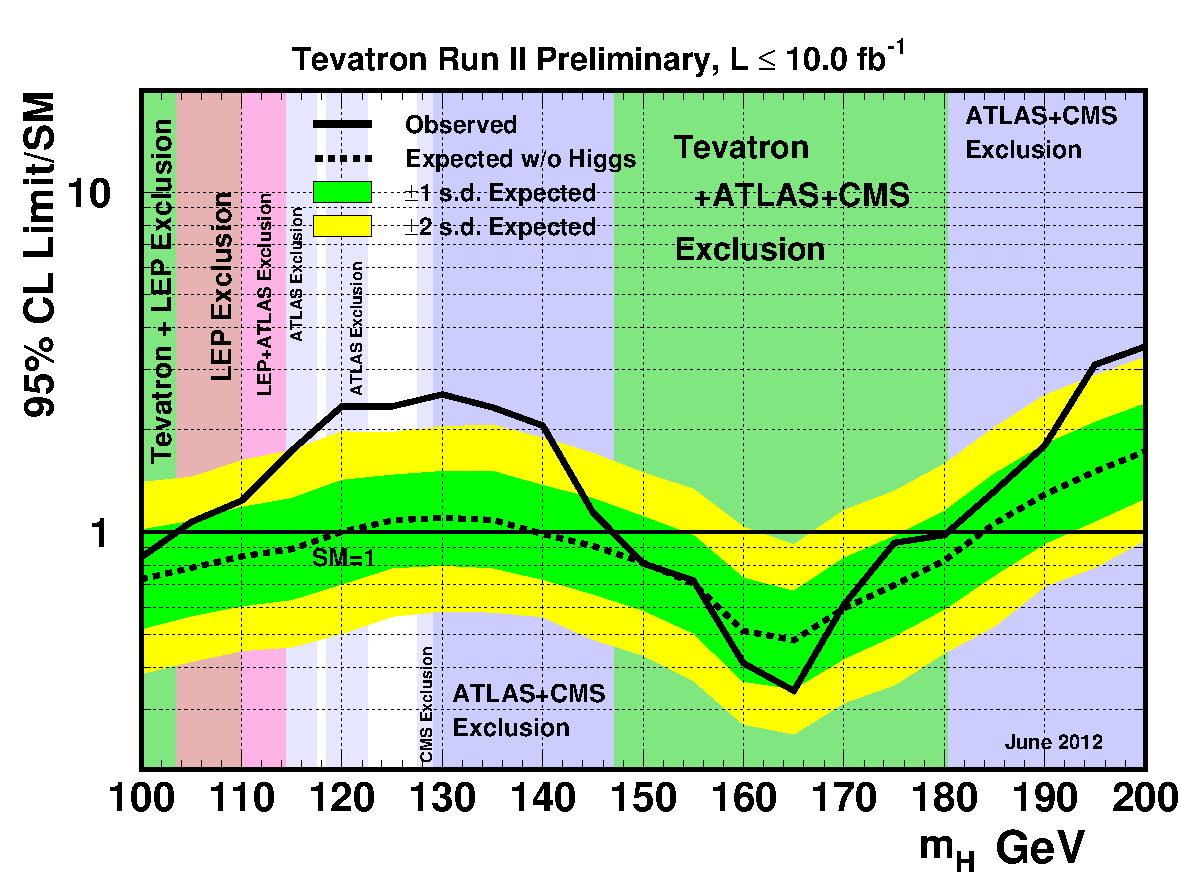
\includegraphics[width=0.8\textwidth]{theory/pheno/tevsmbayes_june2012_withleplhc.pdf}
\caption{The 95\% confidence upper limits on the ratio of Higgs boson production to the SM prediction
as a function of $\mh$.
The dotted line indicates the median expected exclusion assuming no
SM Higgs boson exists while the solid line indicates the observed exclusion obtained 
from the data. Where this line falls below 1, a SM Higgs boson with that mass is excluded at the
95\% confidence level as indicated by the green bands. The other coloured bands indicate 
exclusion limits resulting from direct searches for the SM Higgs boson conducted by other
Collaborations before June 2012. The figure has been altered from its original 
source~\cite{tevhiggscombinations}.}
\label{fig:tevatronlims}
\end{center}
\end{figure}

\subsubsection{Precision Measurements}
Collision data taken at the Tevatron are combined with precision measurements 
of electroweak observables performed at LEP
and by the SLD Collaboration based at SLAC to constrain the mass of the 
Higgs boson. Figure~\ref{fig:blueband} shows the relative chi-squared from a fit
to these data as a function of $\mh$. The minimum of the curve is at 94 GeV
with an experimental uncertainty of +29 and -24 GeV. The theoretical uncertainty
is indicated by the blue band. The yellow bands indicate the excluded regions in 
$\mh$ provided by direct searches for the SM Higgs boson conducted at LEP
and the LHC by March 2012.
\begin{figure}
\begin{center}
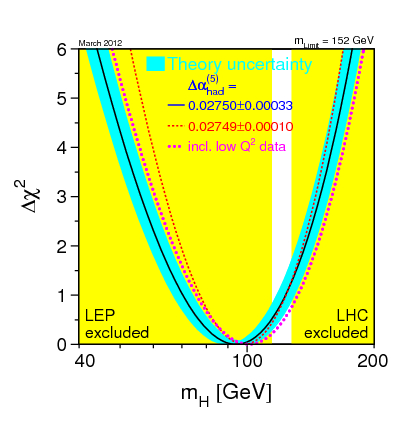
\includegraphics[width=0.6\textwidth]{theory/pheno/w12_blueband.jpg}
\caption{Delta chi-squared from global fit to combined data from CDF, D0, SLD and the LEP
Collaborations as a function of $\mh$~\cite{lepewwgpage}. 
The solid line is the nominal fit with theoretical
uncertainties indicated in blue while the dashed lines indicate alternative theoretical 
prescriptions. The yellow bands indicate the regions excluded at the 95\% confidence level
from direct searches for the SM Higgs boson conducted at LEP and the LHC before March 2012.} 
\label{fig:blueband}
\end{center}
\end{figure}

\subsection{Higgs Boson Production and Decay at the LHC}

At the LHC, protons are accelerated to higher energies than previously available at the 
Tevatron. The increased centre-of-mass energy enhances the 
rate at which Higgs boson production occurs and improves the sensitivity to higher 
masses. The four main mechanisms by which a Higgs boson can be produced
are shown at leading order in Figure~\ref{fig:higgsprodfeyn}.
\begin{figure}[hbtp!]
\begin{center}
%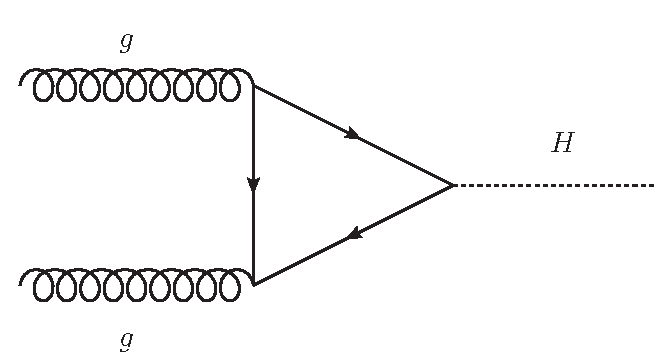
\includegraphics[width=.49\textwidth]{theory/pheno/ggh.pdf}
%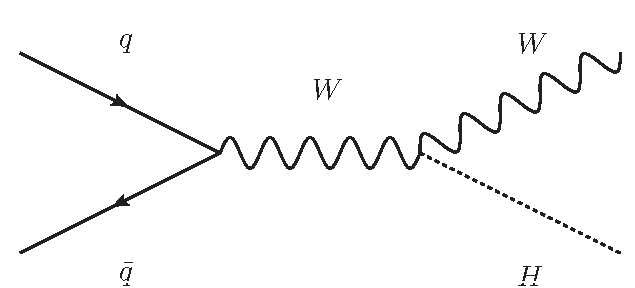
\includegraphics[width=.49\textwidth]{theory/pheno/vh.pdf}\\
%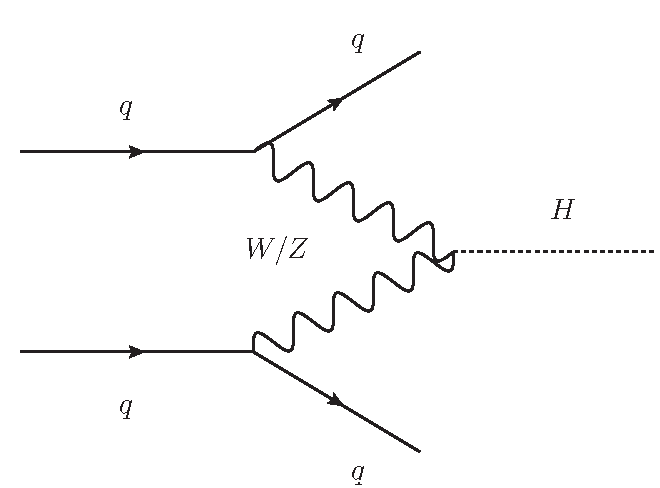
\includegraphics[width=.49\textwidth]{theory/pheno/qqh.pdf}
%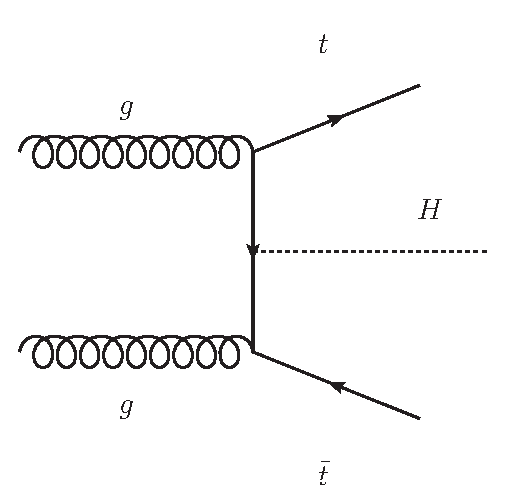
\includegraphics[width=.4\textwidth]{theory/pheno/tth.pdf}
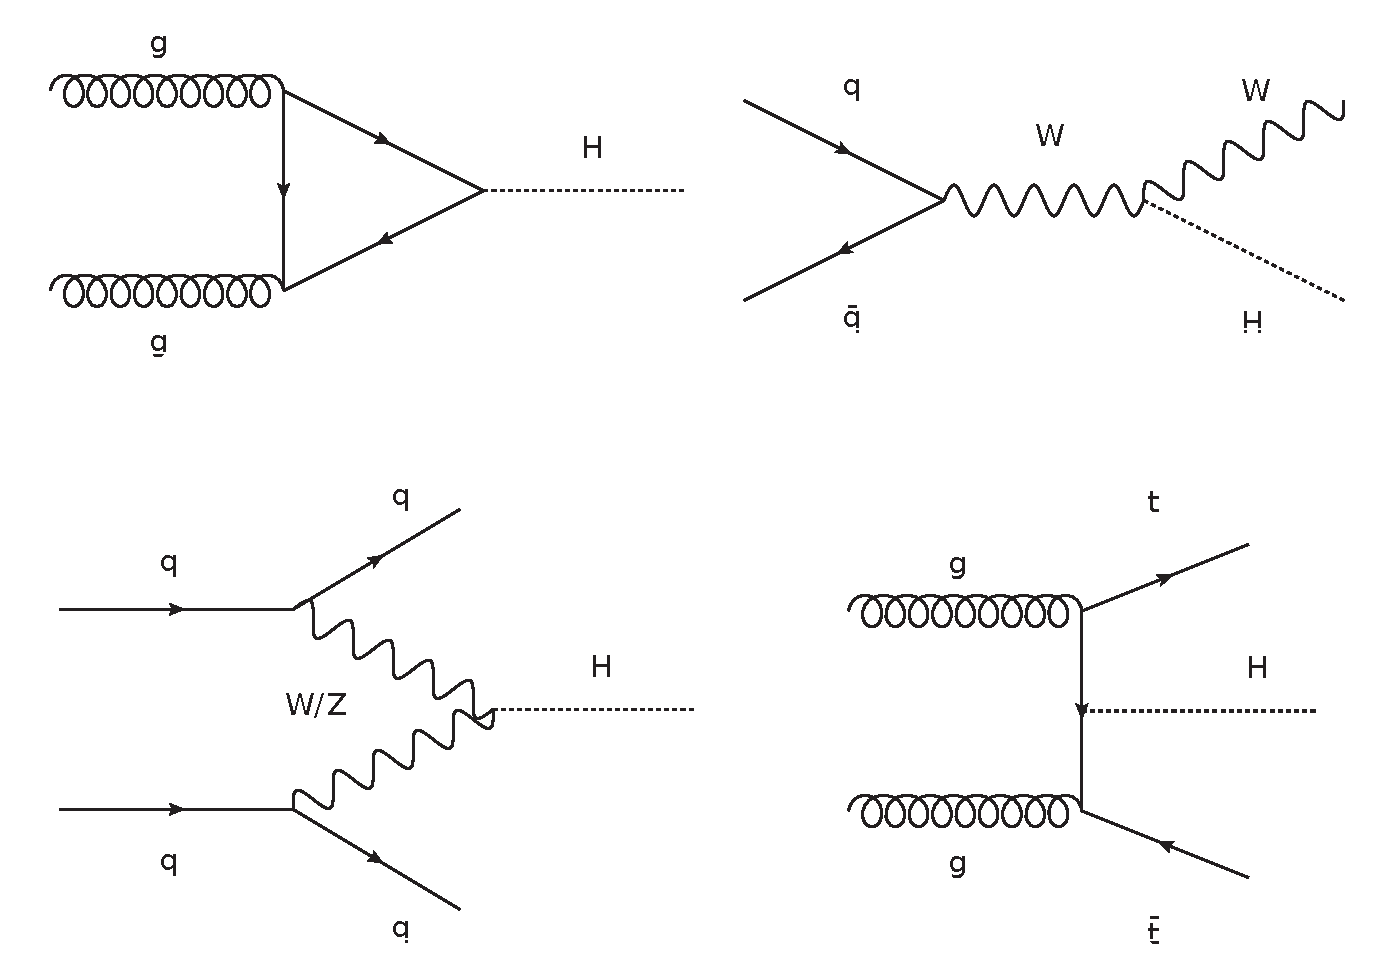
\includegraphics[width=\textwidth]{theory/pheno/allprods_new.pdf}
\caption{Dominant SM Higgs boson production mechanisms: Gluon-gluon fusion (top left),
vector-boson fusion (bottom left), associated production with vector boson (top right) 
and top anti-top quark pair (bottom right).}
\label{fig:higgsprodfeyn}
\end{center}
\end{figure}
The dominant production mechanism is through gluon-gluon fusion ($ggH$). As the gluons
are massless particles, the gluons couple to the Higgs boson via a quark-loop.
The three other production mechanisms which dominate Higgs boson production are 
vector boson fusion ($qqH$) and production in association with 
a $W$ or $Z$ boson ($VH$) or top anti-top quark pair ($ttH$).
Although these modes are at least an order of magnitude smaller in cross-section
than gluon-gluon fusion, their specific topologies 
can be exploited experimentally to enhance the signal over background processes 
(see Chapter~\ref{chap:combinations}).
Figure~\ref{fig:higgsprod} shows the production cross-sections and their theoretical 
errors for the four main production modes of the SM Higgs boson in  
p-p collisions at the LHC~\citep{lhcxswg2011,lhcxswg2012}.
\begin{figure}[hbtp!]
\begin{center}
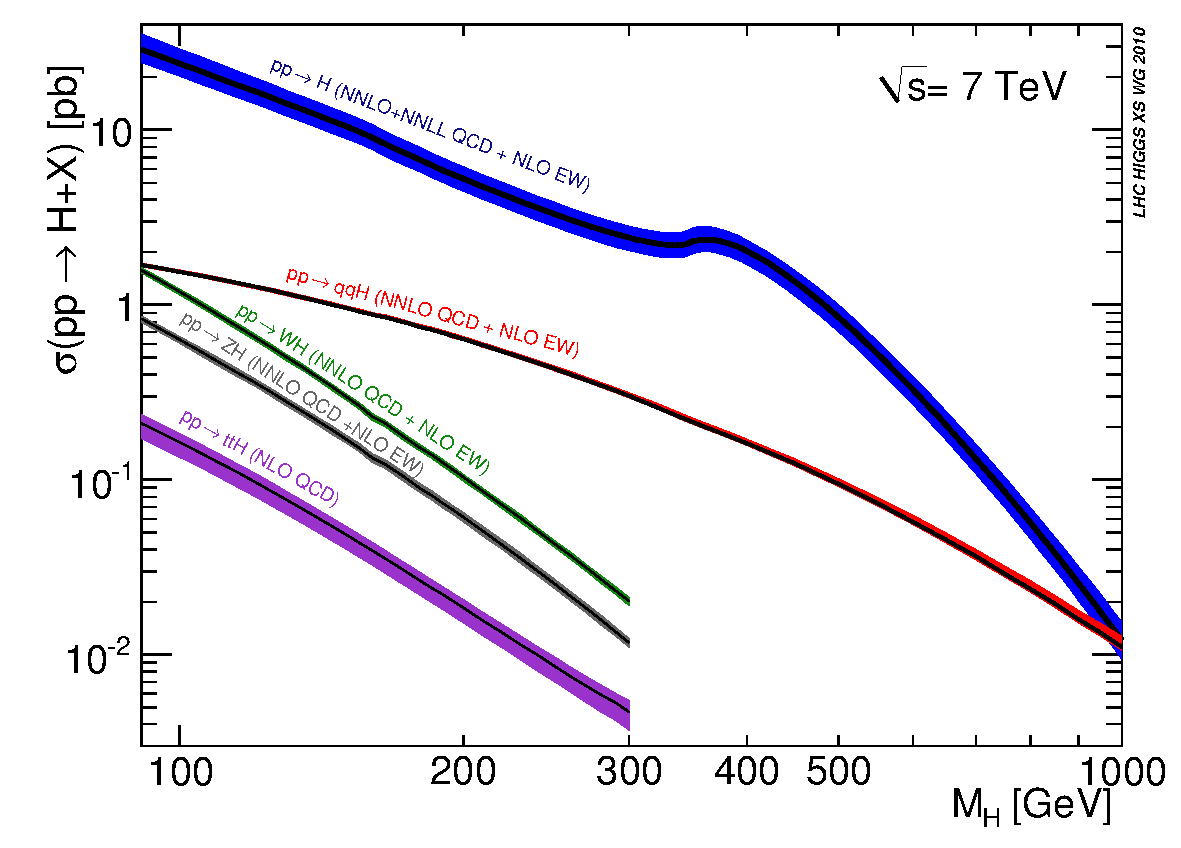
\includegraphics[width=0.8\textwidth]{theory/pheno/Higgs_XS_7TeV.pdf}\\
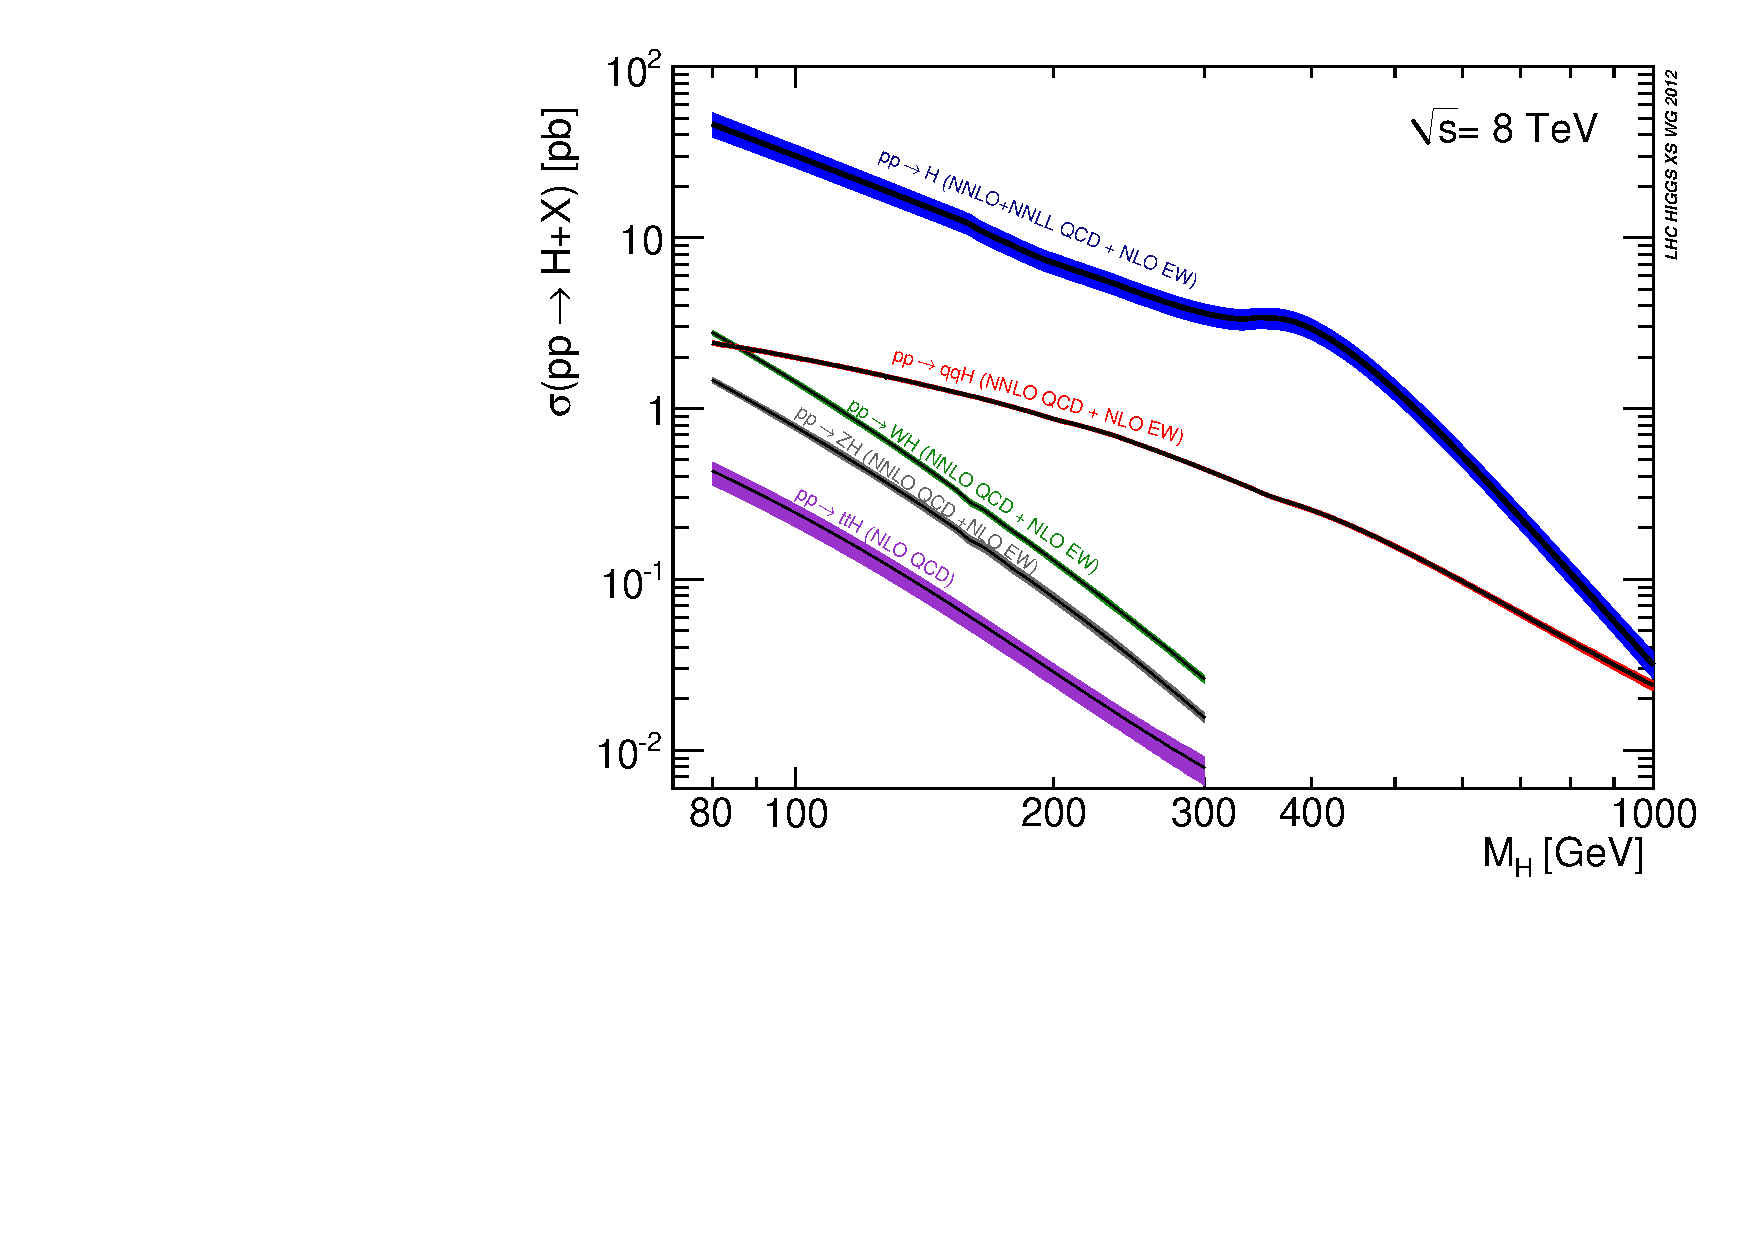
\includegraphics[width=0.8\textwidth]{theory/pheno/Higgs_XS_8TeV_lx.pdf}
\caption{SM Higgs boson production cross-sections at $\sqrt{s}=7~\mathrm{TeV}$ (top)
and 8 TeV (bottom) of the four main production mechanisms, $pp\rightarrow H+X$,
along with their theoretical uncertainties as a function of 
$\mh$~\citep{lhcxswg2011,lhcxswg2012}. The coloured bands indicate the theoretical
uncertainties.}
\label{fig:higgsprod}
\end{center}
\end{figure}
The Higgs boson is an unstable particle so will be observable directly at the LHC
only through its decay products. The relative decay rates (branching ratios) to 
different SM particles vary as a function of the Higgs boson mass.
At low mass, $\mh<135$ GeV, Higgs boson decay to a $b$ anti-$b$ quark pair
dominates. In proton-proton collisions, pairs of $b$-quarks are produced 
frequently making the background levels too high to compete with for an experimental
search. For higher masses, $\mh>180$ GeV, the Higgs boson is heavy enough
to facilitate production of real $W$ and $Z$ bosons which dominate its decay.
As the gluon and photon are massless, they do not directly couple to the Higgs boson
hence these decays are mediated by virtual loops of massive particles.
The branching ratios of the Higgs boson to SM particles are shown as a function
of $\mh$ in Figure~\ref{fig:higgsdecay} (left).

For small $\mh$, the natural width of the SM Higgs boson, $\hwidth$, is several
orders of magnitude smaller than its mass. Figure~\ref{fig:higgsdecay} (right) shows the 
value of the SM Higgs boson total width as a function of its mass.
This means that for decays in which the products are fully reconstructible in particle
detectors, the width of the invariant mass spectrum of the decay products will depend almost entirely
on the experimental resolution. 
In particular the ATLAS and CMS detectors provide excellent energy and momentum resolution 
for electrons, muons and photons.
Despite having lower branching ratios,  the $\Hgg$ and $\Hzzl$ channels
are therefore of particular importance for direct detection of the SM Higgs boson
at the LHC.


\begin{figure}[hbtp]
\begin{center}
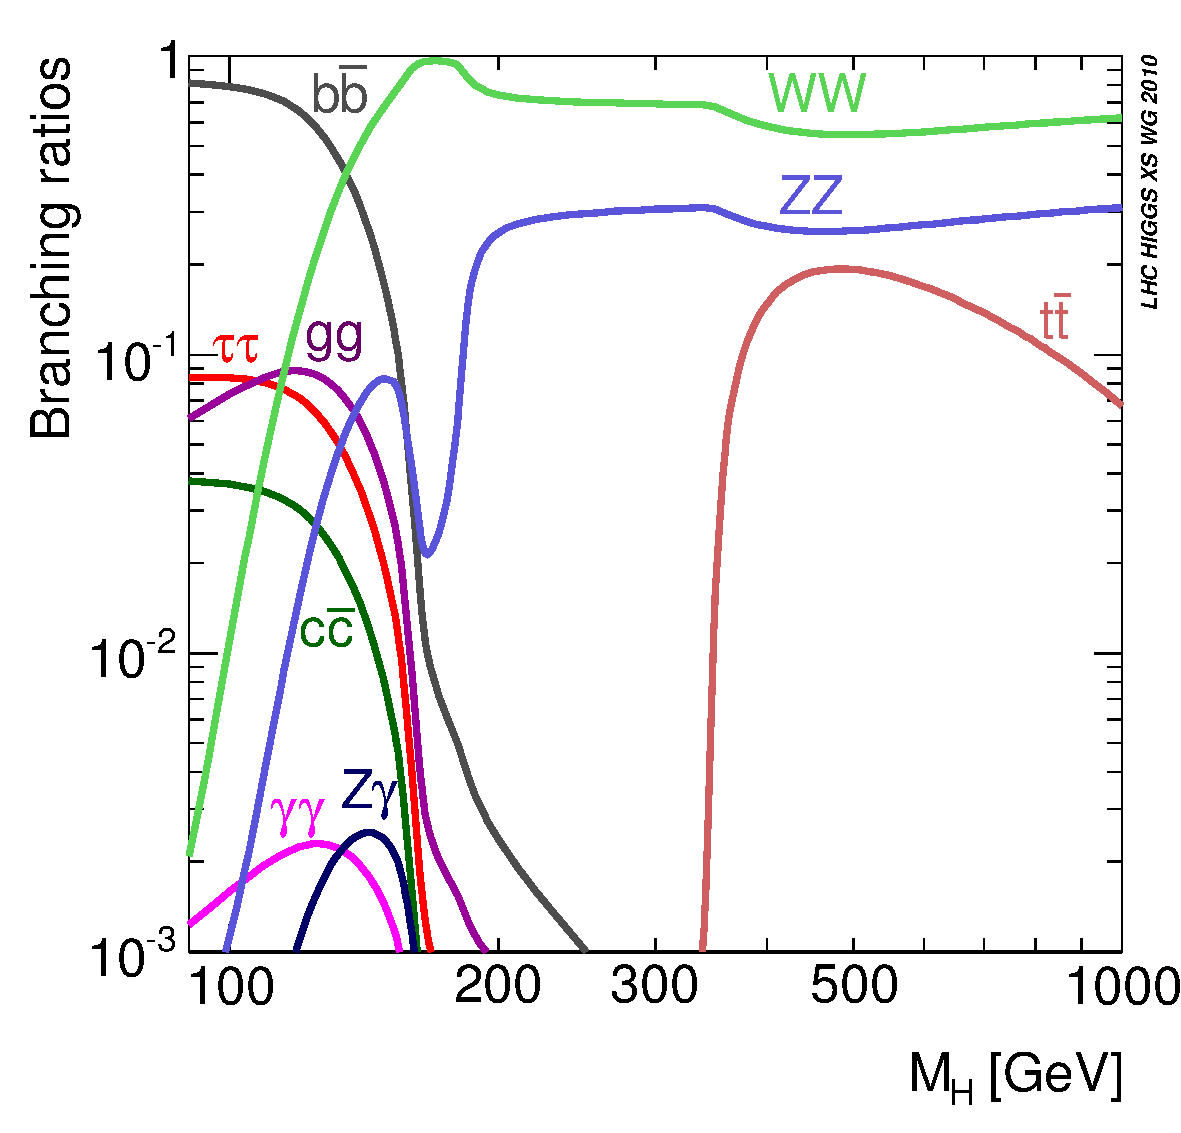
\includegraphics[width=0.49\textwidth]{theory/pheno/YRHXS_BR_fig3.pdf}
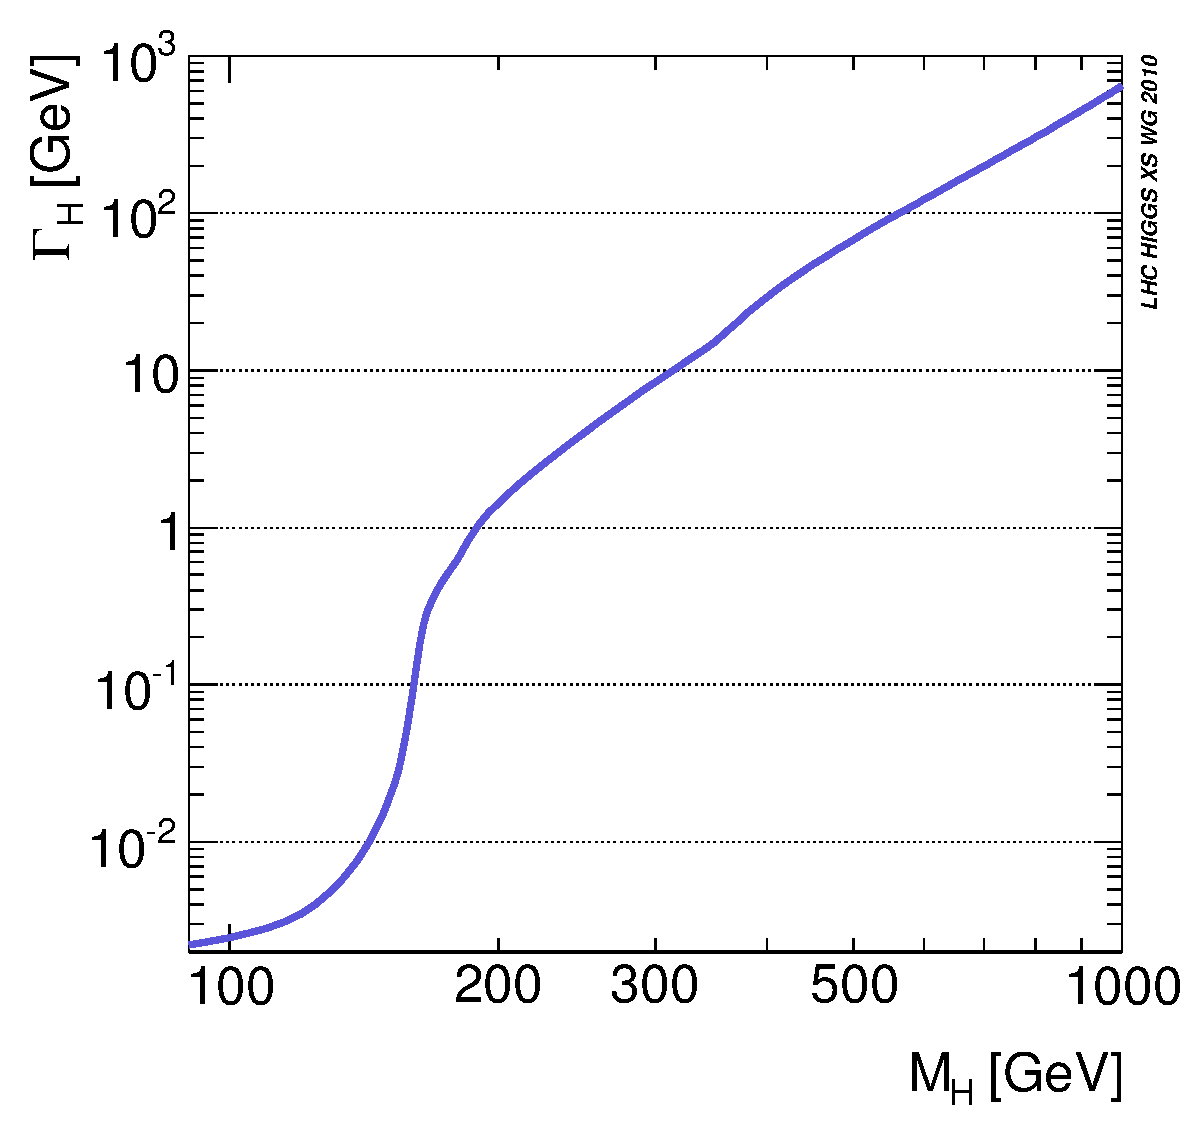
\includegraphics[width=0.49\textwidth]{theory/pheno/YRHXS_BR_fig2.pdf}
\caption{Left: SM Higgs boson production branching ratios for 
the dominant decays as a function of $\mh$. Right: SM Higgs boson total width, $\hwidth$, as 
a function of $\mh$~\citep{lhcxswg2011}.}
\label{fig:higgsdecay}
\end{center}
\end{figure}


\chapter{The LHC and the CMS Detector}
\label{chap:detector}

One of the many physics goals of the LHC is the establishment of the mechanism by which 
the fundamental fermions and bosons acquire mass in the SM. The discovery of the new particle 
announced by the ATLAS and CMS Collaborations in July 2012, if found to be the Higgs boson, will have provided 
a major step towards this goal. This of course could not have been achieved without the use
of the particle detectors designed by those Collaborations. This Chapter is intended to serve as an 
introduction to the CMS detector, being the experiment the author worked at. Section~\ref{sec:cmsdetector}
provides an overview of the components of the CMS detector, paying attention in particular to those 
which are the most relevant for the search for the Higgs boson in the two photon decay mode. 
Section~\ref{sec:l1trigger} will cover work performed by the author, as service to the CMS Collaboration, 
on improving the jet resolution in the GCT component of the L1 trigger. A set of calibrations (derived by 
the author) to be used online during CMS data-taking are described.

\section{The LHC}
The Large Hadron Collider (LHC) at CERN is the only collider experiment, currently in operation, 
designed to study physics at the TeV scale. The collider is an octagonal 
ring, 27 km in circumference, hosted in the former LEP tunnel in France/Switzerland.  
Both proton-proton (pp) and heavy ion (PbPb) collisions are
studied as part of the LHC physics programme with the former used 
for direct searches for new physics. Proton beams are formed inside the proton synchrotron
from bunches of protons 50 ns apart with an energy of 26 GeV. The protons are then accelerated in the 
super proton synchrotron to 450 GeV before being injected into the LHC. 
Around 1200 superconducting dipole magnets maintain two beams of protons accelerating around 
the ring in opposite directions before being collided at one of the sites of the four major experiments;
ALICE~\citep{aliceexperiment}, ATLAS~\citep{atlasexperiment}, CMS~\citep{cmsexperiment}
and LHCb~\citep{lhcbexperiment}. Figure~\ref{fig:lhcring} is a cartoon of the accelerator 
indicating the sites of the four experiments.

\begin{figure}[htb!]
\begin{center}
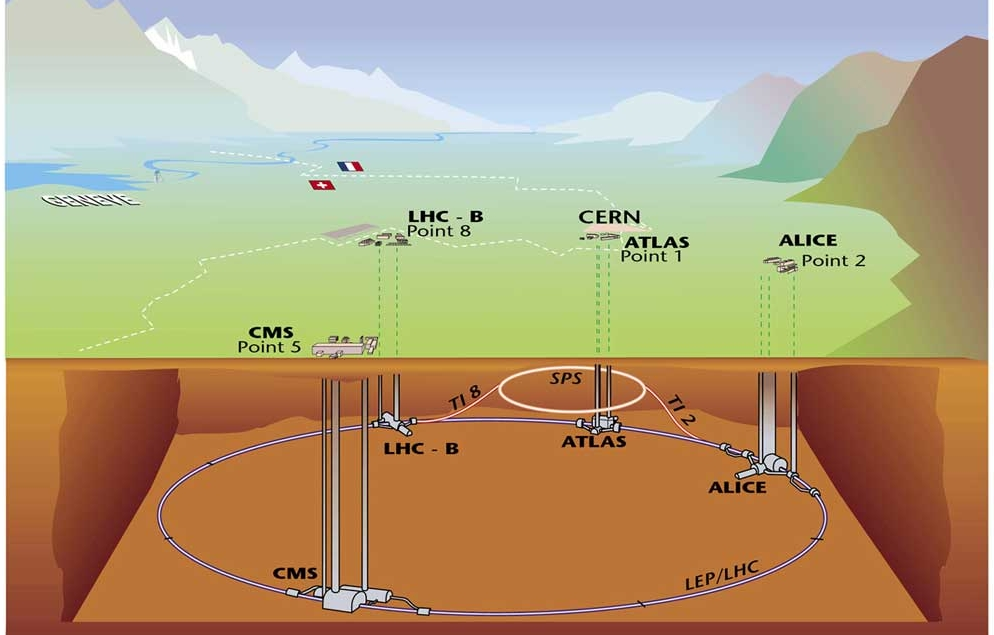
\includegraphics[width=0.8\textwidth]{detector/CERN.jpg}
\caption{LHC accelerator ring. The relative locations of the four main experiments 
are indicated along with their points of access to the beam.}
\label{fig:lhcring}
\end{center}
\end{figure}

The first major physics run began in May 2010 with a centre of mass energy 
$\sqrt{s}=7~TeV$ and continued until November providing a dataset of $44pb^{-1}$.
The LHC resumed collisions in April 2011 delivering a further $6fb^{-1}$ by the end
of October. The centre of mass energy was increased to $\sqrt{s}=8~TeV$ for the 2012 pp 
collision run, improving the sensitivity of searches for new physics. A total of
$6fb^{-1}$ of 8 TeV data were taken by July 2012 which were combined with earlier data resulting
in the discovery of the new boson reported by ATLAS and CMS Collaborations at the ICHEP conference that year. 

\section{The CMS Detector}
\label{sec:cmsdetector}
The Compact Muon Solenoid (CMS) detector is one of two general purpose detectors at 
the LHC designed to search for new physics. 
Among the wide range of physics programs at CMS, the search for the SM Higgs boson 
has a high priority. The decay rates of the SM Higgs boson in different 
channels vary dramatically as a function of its mass ($\mh$). A key feature of the experiment's design
was, therefore, the necessity to maintain a high sensitivity to the SM Higgs for a wide range of masses in as many 
decay channels as possible. To achieve this, several detector components are layered around 
the beam axis to reconstruct many types of particle produced at the interaction point.
Each component consists of a cylindrical barrel section and two endcaps 
to provide an almost hermetic coverage of the outgoing particle flux.


The tracker, providing measurements of the momentum of charged particles and the location of 
primary and secondary vertices (from decays of heavy flavour mesons), is the first layer of detection.
This is followed by the electromagnetic calorimeter which is used to measure
energy deposited in electromagnetic showers from particles such as electrons and photons. 
The hadronic calorimeter (HCAL) complements this by providing energy measurements of 
sprays of hadrons, known as jets, which deposit energy through nuclear interactions. 
The HCAL is a sampling calorimeter in that the active material (plastic scintillators)
are sandwiched between dense absorbing material to increase the depth of the calorimeter to
around 11 radiation lengths. The addition of the forward calorimeter (HF) extends the HCAL
coverage in the forward regions.  
The tracker and calorimeters are situated within a 4T axial magnetic field 
provided by the superconducting magnet surrounding them.
The magnetic flux return is implemented within the  muon detector systems which lie outside 
the superconducting coil and form the outermost detection layers. Muons deposit very little energy 
throughout the detector and can carry on into the surrounding cavern.
The barrel muon system is constructed from layers of drift-tubes (DT) interleaved with 
resistive plate chambers. The combination of the two provides high resolution
timing and hit positions which are used to determine the trajectory of muons both from
p-p collisions and cosmic sources for calibration. For the endcaps, the DTs are replaced
with cathode strip chambers as the higher flux of particles along the beam line
requires the use of radiation hard components.
% ------------------------------------------------------------------------------------

CMS uses a right-handed Cartesian coordinate system with the origin at the 
interaction point and the $z$-axis pointing along the beam axis. The $x$-axis points towards 
the centre of the LHC ring and the $y$-axis points vertically upwards. The azimuthal angle, 
$\phi~\epsilon~[-\pi,\pi]$, is defined with respect to the $x$-axis in the 
transverse ($x-y$) plane. The polar angle $\theta$ is measured from the $z$-axis. Commonly,
the direction of an outgoing particle is defined by $\phi$ and its pseudo-rapidity $\eta$ 
defined as 
\begin{equation}
	\eta=-\log \tan \left( \frac{\theta}{2} \right).
\end{equation}
As hard collisions produce high momentum particles travelling perpendicular to the beam line, 
particles are often characterised
by the magnitude of the projection of their momenta onto the transverse plane, 
$\pt=\sqrt{p_{x}^{2}+p_{y}^{2}}$.
Similarly, the transverse energy is defined as $E_{T}=E\sin\theta$.
Figure~\ref{fig:cms} shows the geometry of the CMS detector and its major components. 

\begin{figure}
\centering
	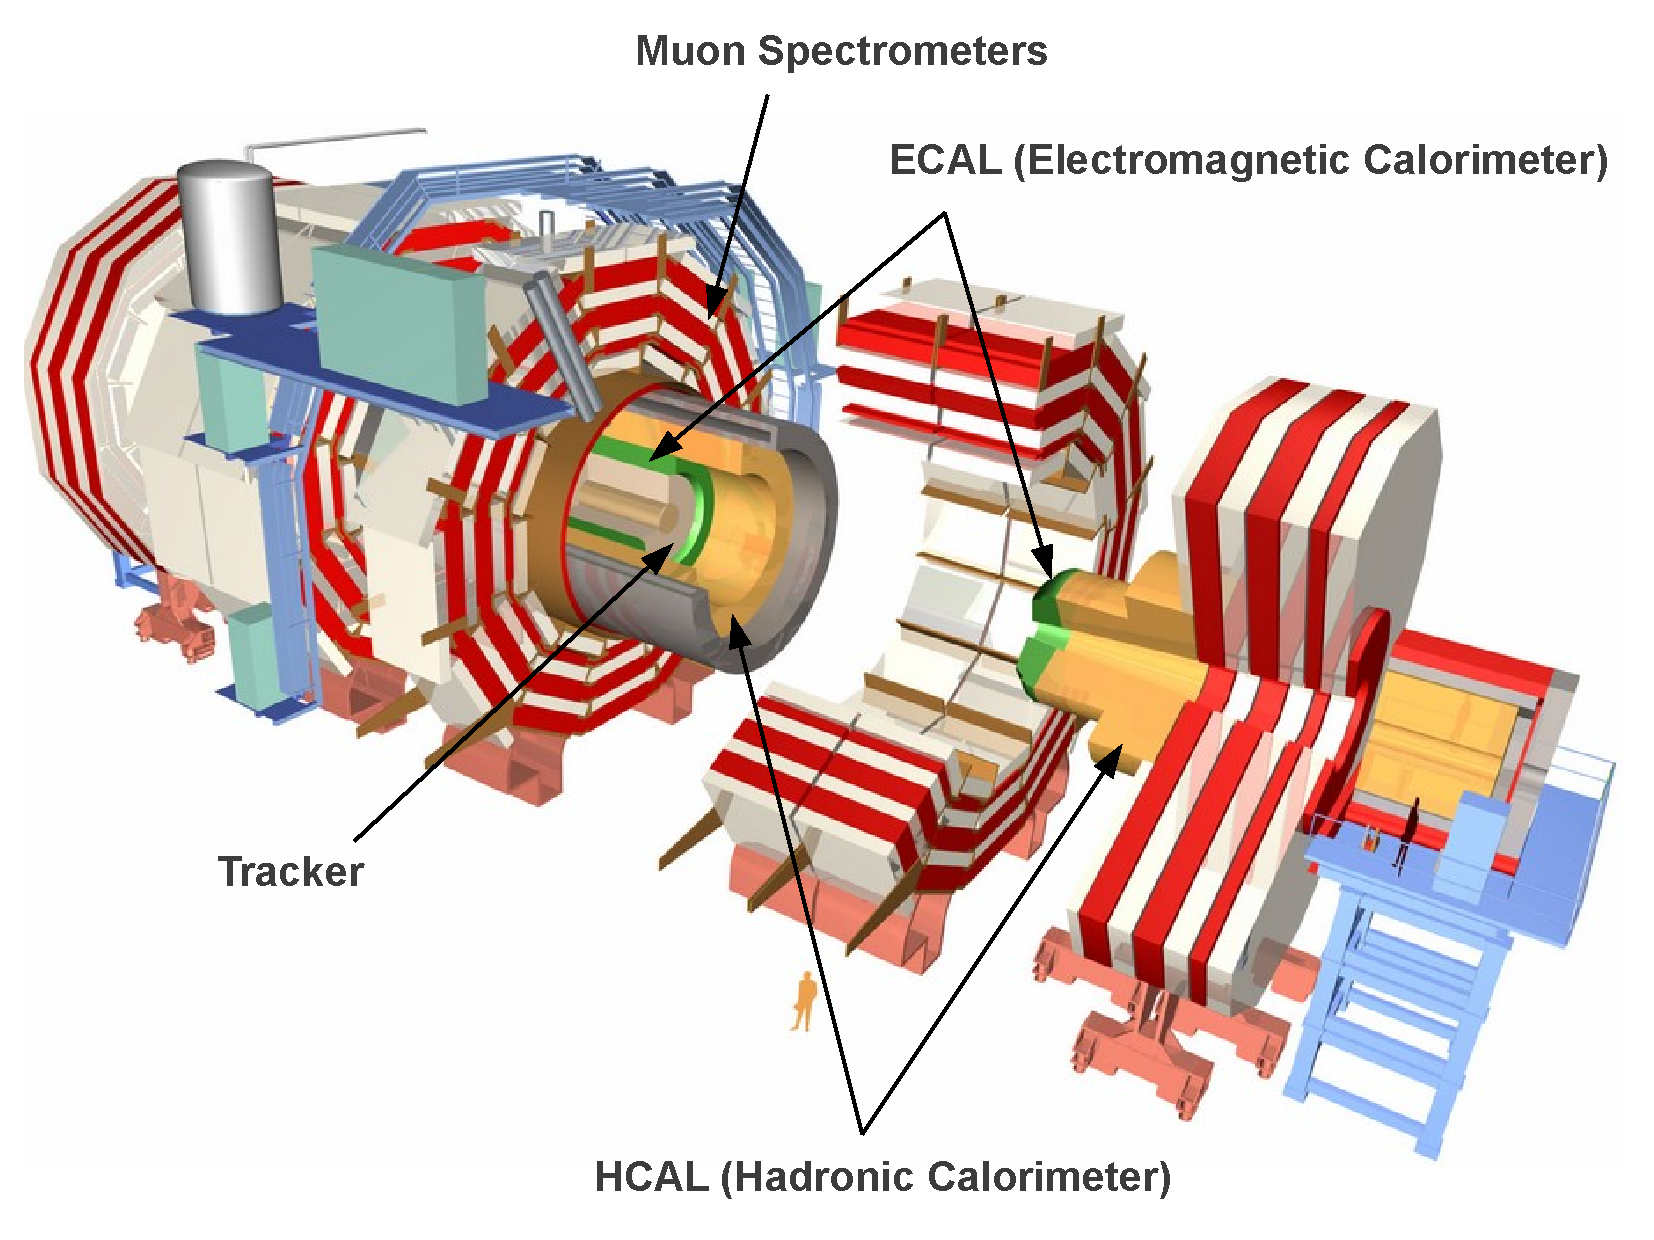
\includegraphics[width=0.8\textwidth]{detector/cmsdetector}
	\caption{Diagram of the CMS Detector. The arrows indicate the main detector elements. 
	The figure has been altered from its original source~\citep{cmspub}.}
	\label{fig:cms}
\end{figure}

\subsection{Tracker}
The CMS tracker is designed to reconstruct charged particle tracks 
which are ubiquitous in high energy 
p-p collisions. The tracker provides precise measurements of 
observables such as the momentum of charged particles and the location of the
vertex at which they are produced.
In addition to the high level of granularity required to make such measurements, the 
high rate of interaction at LHC requires a fast response from the tracking 
elements. 
The tracker is formed of a pixel detector component encased by layers of silicon strip detectors.
The pixel detector is the closest tracking element to the interaction point. 
It is a composite of 66 million individual silicon pixels, $100\mu m \times 150 \mu m$ in size,
forming three cylindrical layers around the beam line and two forward disks. 
The resolution of the pixel detector is around 10 $\mathrm{\mu}$m in the $\hat{r}$ and $\hat{\phi}$ 
direction and 17 $\mathrm{\mu}$m in $\hat{z}$~\citep{trckAC}. 
Outside the pixel detector, ten cylindrical layers of silicon strip detectors (TIB/TOB) 
and twelve discs (TID/TEC) extend the tracking system out to a radius of 120cm from the 
beam line. The tracker geometry, as shown in Figure~\ref{fig:trackergeom}, covers a pseudo-rapidity 
range $|\eta| < 2.5$.

\begin{figure}
	\centering
	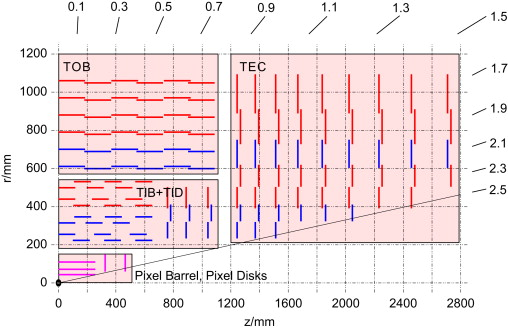
\includegraphics[width=0.9\textwidth]{detector/trcker/tracker_col.jpg}
	\caption{Cross-section of the pixel and silicon strip detector 
	components of the CMS tracker~\citep{Weber201159}.}
   \label{fig:trackergeom}
\end{figure}

By making multiple precise measurements throughout the tracker system, the trajectories (tracks) of charged 
particles can be reconstructed.
Tracks are associated to a common point of origin (primary vertex) by grouping those which are separated
by less than 1cm in the $z$ coordinate of the point of closest approach to the beam line.
The vertex resolution is dependant both on the number of tracks associated to the vertex and
their average transverse momenta ($\bar{p}_{T}$). The resolution was measured in early data from 2010
by splitting tracks associated to a vertex randomly into two groups with equal kinematic distributions.
The difference between the vertex locations calculated from the two groups was used to provide an estimate 
of the resolution~\citep{TRK-10-005}.
Figure~\ref{fig:vtxreso} shows the resolution in $z$ as a function of the track multiplicity
measured in data and simulation. The simulation provides a good description of both the trend with 
number of associated tracks and the improvement in resolution with $\bar{p_{T}}$ in the data. 

\begin{figure}
\begin{center}
	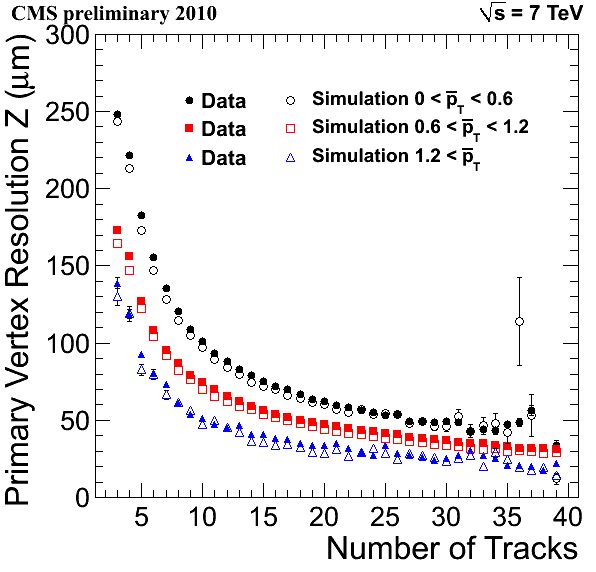
\includegraphics[width=.6\textwidth]{detector/trcker/zresotrcker.png}
	\caption{Resolution of vertex $z$-position as a function of the number 
	of tracks associated to the vertex measured in simulation and 
	2010 data~\citep{TRK-10-005}.
 	The resolution is given for three different average track momenta.}
	\label{fig:vtxreso}
\end{center}
\end{figure}

\subsection{Electromagnetic Calorimeter}
The electromagnetic calorimeter (ECAL) is used to reconstruct energy deposits in electromagnetic showers 
from particles such as electrons and photons. 
It is constructed from high density lead tungstate (PbWO$_{4}$) crystals which
form a barrel section (EB) and two endcaps (EE) outside the tracker. 
Two lead plates in front of a fine grained silicon strip detector are situated just before the 
endcaps forming the ECAL pre-shower (PS). 
Photons travelling at high $\eta$ will convert in the lead and the resulting electron-positron pair
will produce tracks which can be used to pinpoint the position of the incoming photon. The additional
information obtained using the two layers can be used to distinguish prompt photons from those produced
in neutral pion decays.

The ECAL is designed to cover a pseudo-rapidity range of $|\eta | < 3$. 
The crystals are arranged to form modules which surround the beam line in a non-projective geometry:
the gaps between crystal modules are offset by 3$^{\circ}$, beyond the interaction point, with respect to 
the trajectories of particles which produced at the centre of the interaction point. 
Electrons and photons deposit most of their energy within 
the crystals as the depth of the crystals is equivalent to 25.8 radiation lengths~\citep{TDR1}. 
Electromagnetic showers produced by the interaction of electrons and photons in the ECAL crystals
produce scintillation light which is collected to measure the energy of the particle. 
The scintillation output of the crystals is, however, low and temperature dependant 
($\sim$ 2.1\%/K at the ECAL operating temperature of 291 K). 
Avalanche photo-diodes (APDs) and vacuum 
photo-triodes (VPTs) are used to collect the scintillation light and amplify the signal in the 
calorimeter barrel and endcaps respectively. 
These technologies are chosen to withstand the high magnetic field inside CMS.
For the endcaps, VPTs are used as they are less sensitive to the high radiation conditions  
in the forward regions. Around 4.5 photo-electrons per MeV are produced in both APDs and VPTs. 

The energy resolution of the ECAL can be parametrised as the combination of three 
uncorrelated sources as given in equation~\ref{eqn:resofit}.
The parameters $a$, $b$ and $c$ are the stochastic, noise and constant contributions respectively. 
These constants have been derived from test-beam data~\citep{AN-06-140}.
The stochastic term ($a=2.83\pm0.3\%$) is very low for lead tungstate since the shower 
can be mostly contained within the crystals.
As the noise term ($b=$124 MeV) is determined by the electronics, 
it is mostly the constant term ($c=0.26\pm0.04\%$) which will limit the ECAL accuracy at 
high energies. Maintaining a high resolution 
over the long term running of the LHC will allow for reconstruction of high energy photons, 
such as those produced by $H \rightarrow \gamma\gamma$ decays.
\begin{eqnarray}
\left( \frac{\displaystyle \sigma_{E}}{\displaystyle E} \right)^ 2 
	& = & \left( \frac{\displaystyle a}{\displaystyle \sqrt{E}} \right)^ 2 
  	+ \left( \frac{\displaystyle b}{\displaystyle {E}} \right)^ 2 + c^ 2
\label{eqn:resofit}
\end{eqnarray}


\subsubsection{Electron and Photon Reconstruction}

Electron and photon candidates are formed by clustering deposits of 
energy caused by electromagnetic showers in the ECAL. For unconverted 
photons, these clusters will likely be well localised in $\eta$ and $\phi$
around the incident photon. However, for photons which convert in the material in front of the 
calorimeter, the resulting electron-positron pair will deposit energy across several regions
of the calorimeter. In the presence of the axial magnetic field, 
electrons radiate bremsstrahlung photons causing deposits which are 
spread over a wide range in $\phi$ while being fairly narrow in $\eta$.
This characteristic is exploited by the ``Hybrid'' clustering algorithm 
used to reconstruct high energy electrons and photons in
the ECAL barrel~\citep{cseez}. 
The values of the particular thresholds used for seeding clusters were tuned providing
an efficiency for electrons with $p_{T}>7~GeV$ greater than 99\%~\citep{dfutyan}.
Figure~\ref{fig:hybridclustering} is an illustration of the Hybrid clustering algorithm.
The algorithm proceeds as follows;
\begin{itemize}
 \item Step 1: A seed crystal is determined to be a single crystal in the barrel with the highest
 $E_{T}$ satisfying $E_{T}>1~GeV$.
 \item Step 2: $1\times3$ ($\phi\times\eta$) crystal dominoes are formed with their central crystal 
 aligned with the seed crystal in $\eta$. If the energy contained in the $1\times3$ domino is 
 larger than 1 GeV, the domino is extended by two crystals in $\eta$. A maximum of 10 dominoes are 
 added in each direction in $\phi$ starting from the seed crystal forming a sub-cluster.
 \item Step 3: Dominoes containing less than 100 MeV are removed and the remaining dominoes are 
 grouped into sub-clusters providing each seeding domino for a sub-cluster contains more than 350 MeV. 
 The final group of sub-clusters form a supercluster for the electromagnetic object.
\end{itemize}

\begin{figure}
\begin{center}
	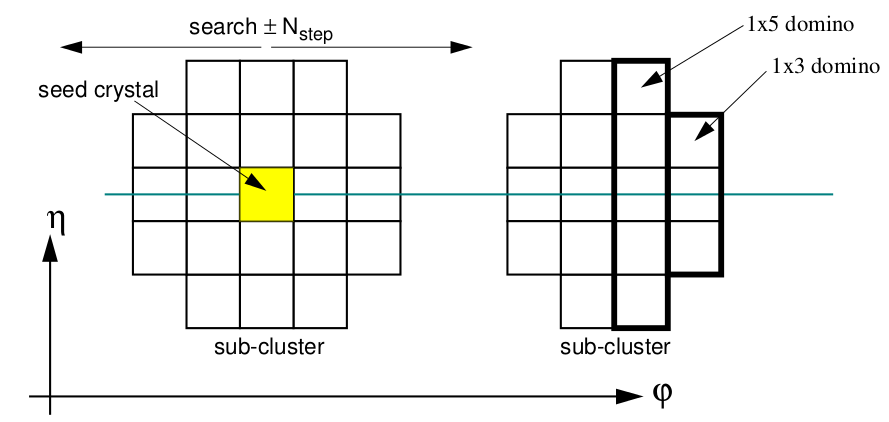
\includegraphics[width=0.8\textwidth]{detector/ecal/clustering.png}
	\caption{Sub-cluster construction of the Hybrid algorithm used to reconstruct photons and 
	electrons in the ECAL barrel.}
	\label{fig:hybridclustering}
\end{center}
\end{figure}

In the ECAL endcaps, superclusters are built using the ``Multi5$\times$5'' algorithm which 
connects overlapping 5$\times$5 grids of crystals whose positions lie within 
0.3 radians in $\phi$~\citep{AN-09-164}. 
Additional information is used from the PS to enhance the energy reconstruction in the endcaps. 

Superclusters are associated to electron candidates 
where a track can be reconstructed from
compatible hits in the tracker using a Gaussian sum filter algorithm~\citep{GSF_Electron_Reconstruction_CMS}.  
This provides an additional measure of the electron's momentum which is used 
to improve the resolution of the electron energy.
Aside from this, the reconstruction of photons and electrons is identical which is an 
important feature allowing for data driven calibrations and validations of photons using 
electrons such as those described in Chapter~\ref{chap:hgg}.


\subsubsection{Laser Calibration}

ECAL crystals suffer from loss of optical transmission when irradiated through 
the formation of crystal-lattice defects which absorb some of the scintillation light. Annealing
acts to balance the damage from radiation which results in an equilibrium optical 
transmission which is dose-dependant~\citep{TDR1}. 
At the LHC, the dose varies during each run. This requires that the time varying optical transmission of the ECAL 
crystals be monitored to asses the impact on energy measurements.
The crystal transparency is monitored by comparing the relative transmission in blue laser light (440 nm), 
which is close to the scintillation emission peak, to infra-red (796 nm), which is far from the 
peak and relatively unaffected by the radiation damage.
Figure~\ref{fig:trans} shows the relative response to the blue laser of the monitoring system
averaged over all the crystals in bins of $|\eta|$ throughout the 2011 data taking 
runs~\citep{CMS-DP-2012-007}. 
The time dependence of the response is stronger at higher values of $|\eta|$ due to the larger flux
of particles along the beam axis.

\begin{figure}
	\centering
	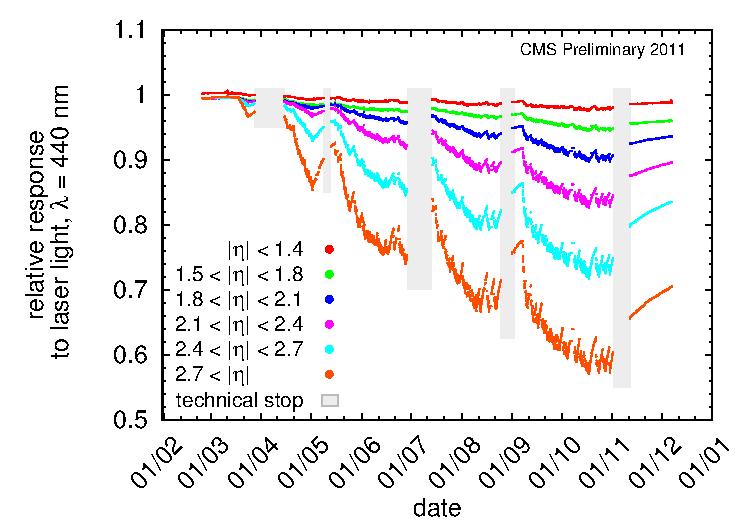
\includegraphics[width=0.8\textwidth]{detector/ecal/laser.pdf}
	\caption{Relative ECAL crystal response to blue laser light (440 nm) in bins of pseudo-rapidity, 
	for the 2011 data taking period. The grey bands indicate periods during which there was no beam.}
	\label{fig:trans}
\end{figure}

The response of the crystals measured using the laser monitoring system is used to calibrate 
the energy reconstruction of the ECAL. These calibrations are validated in $W\rightarrow e\nu$ data events
by comparing the electron energy ($E$) as measured by the ECAL to the momentum 
($p$) of the electron measured in the tracker~\citep{CMS-DP-2012-007}. 
Figure~\ref{fig:scaleeop} shows the relative variation in the ratio $E/p$ as a function of time 
throughout 2011. A stable scale is achieved through application of the laser calibrations.

\begin{figure}
	\centering
	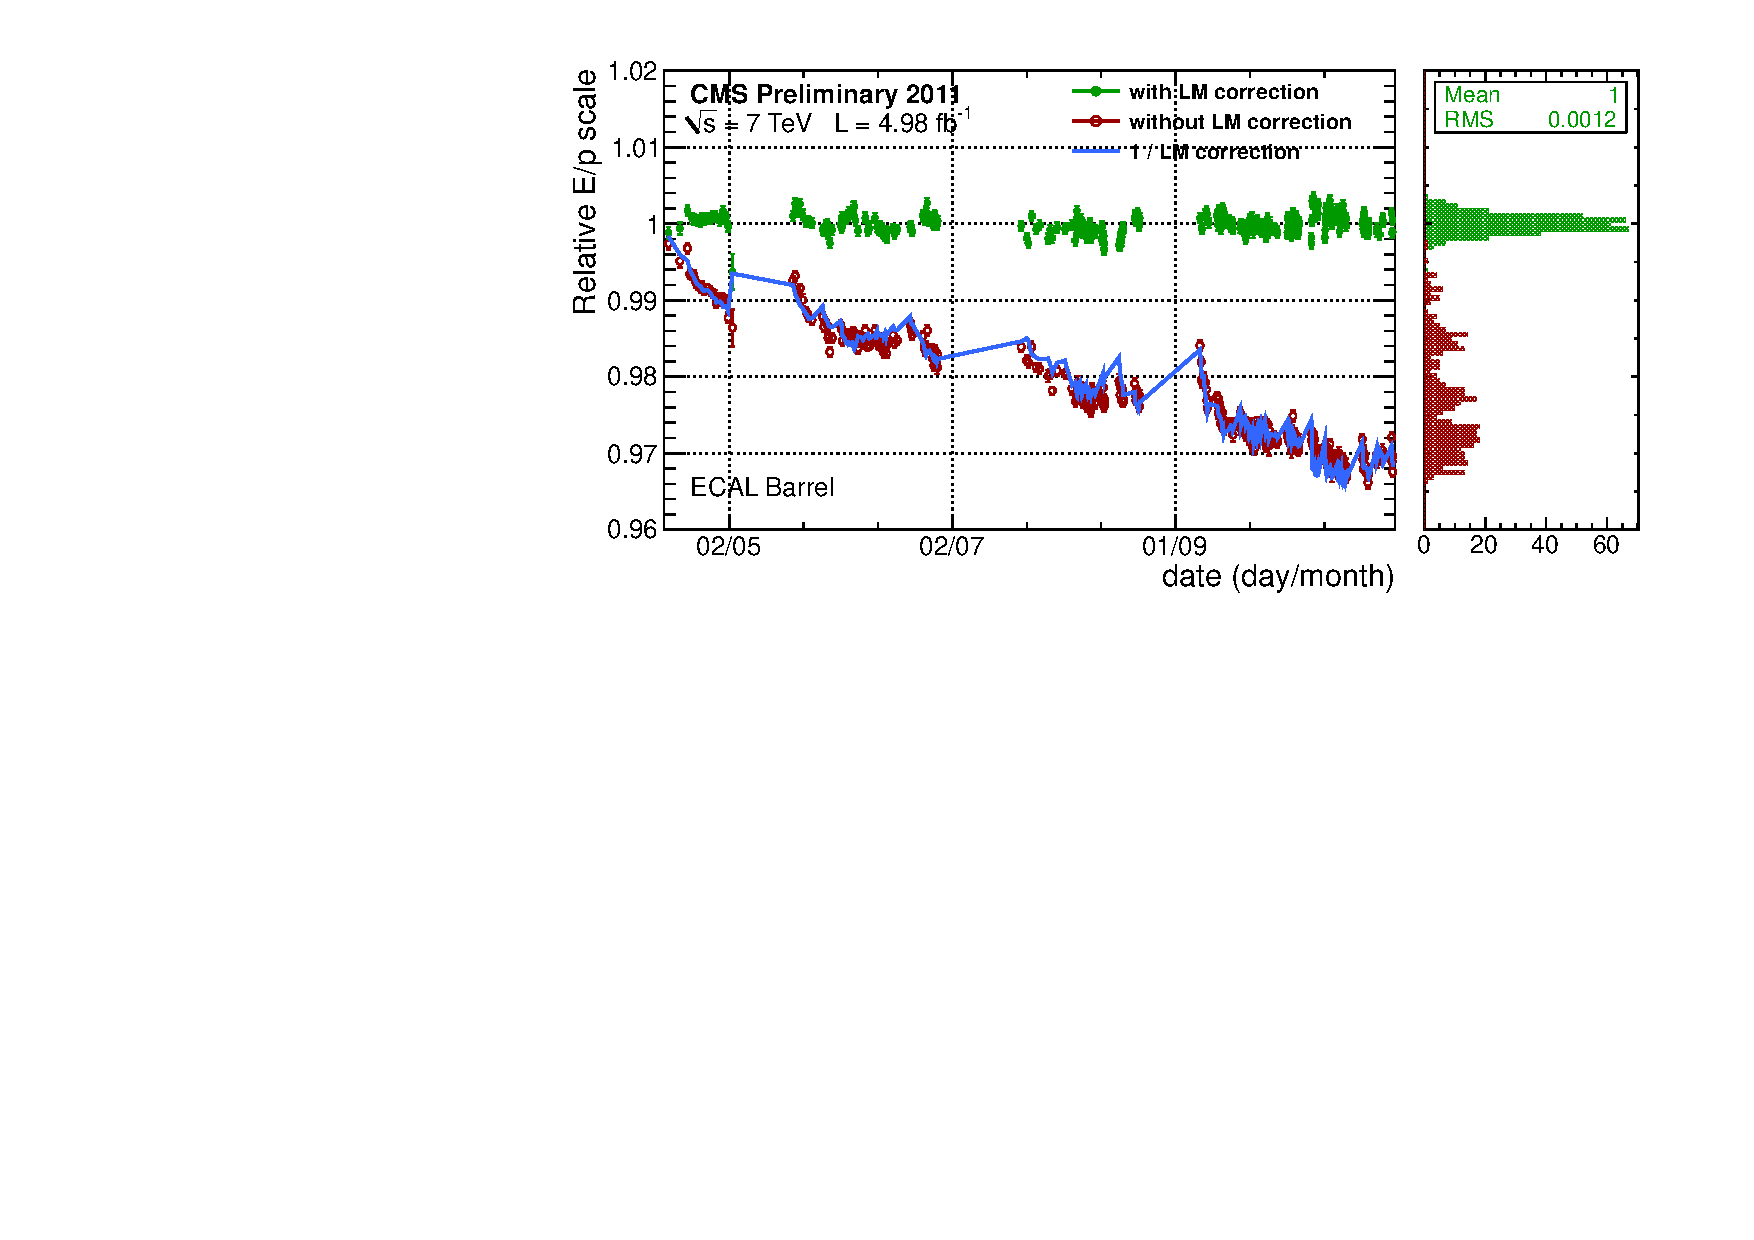
\includegraphics[width=\textwidth]{detector/ecal/scaleeop.pdf}
	\caption{Ratio $E/p$ in electrons reconstructed in the ECAL Barrel 
	from $W\rightarrow e\nu$ events in 2011 data as a function of time before 
	and after applying transparency corrections from the laser monitoring (LM) system. 
	The blue line indicates the correction applied per point averaged over all crystals used in the electron
	energy measurement.}
	\label{fig:scaleeop}
\end{figure}

\subsection{Shower-shape and Isolation}
In addition to providing a measurement of the energy of incoming electromagnetic particles,
the ECAL's fine granularity provides additional information which can be used to characterise
the supercluster and distinguish prompt electrons and photons from fakes.  
The shape of the electromagnetic shower can be described by the ratio of the energy contained
in the central $3\times3$ cluster surrounding the seed crystal to the total energy of the supercluster
($\rnine$). Superclusters associated with real unconverted photons will typically have larger value of 
$\rnine$ than those which are in reality due to narrow $\pi^{0}$ decays. Another common variable used
for identification is the energy weighted crystal width of the sub-cluster used to seed the supercluster  
$\sigieie$, 
\begin{equation}
\sigieie = \frac{\sum_{i}w_{i}(\eta_{i}-\eta_{sc})^{2}\Delta\eta^{2}_{xtal}}{\sum_{i}w_{i}},
\end{equation}
where $\eta_{sc}$ is the pseudo-rapidity of the seed crystal, $\Delta\eta_{xtal}$ is the crystal width
and $w_{i}$ is the crystals weight determined as $w_{i} = \mathrm{max}\left\{0,4.7+\log(E_{i}/E_{tot})\right\}$.
Prompt photons will tend to have a more localised cluster leading to lower values of $\sigieie$. 
The distributions of $\rnine$ and $\sigieie$ are shown for a simulated sample of 
superclusters identified as photons from real and fake sources in Figure~\ref{fig:showershape}.
The two distinct peaks in the $\sigieie$ distribution are due to the different superclustering algorithms 
used in the barrel and endcaps.

\begin{figure}[hbt!]
\begin{center}
	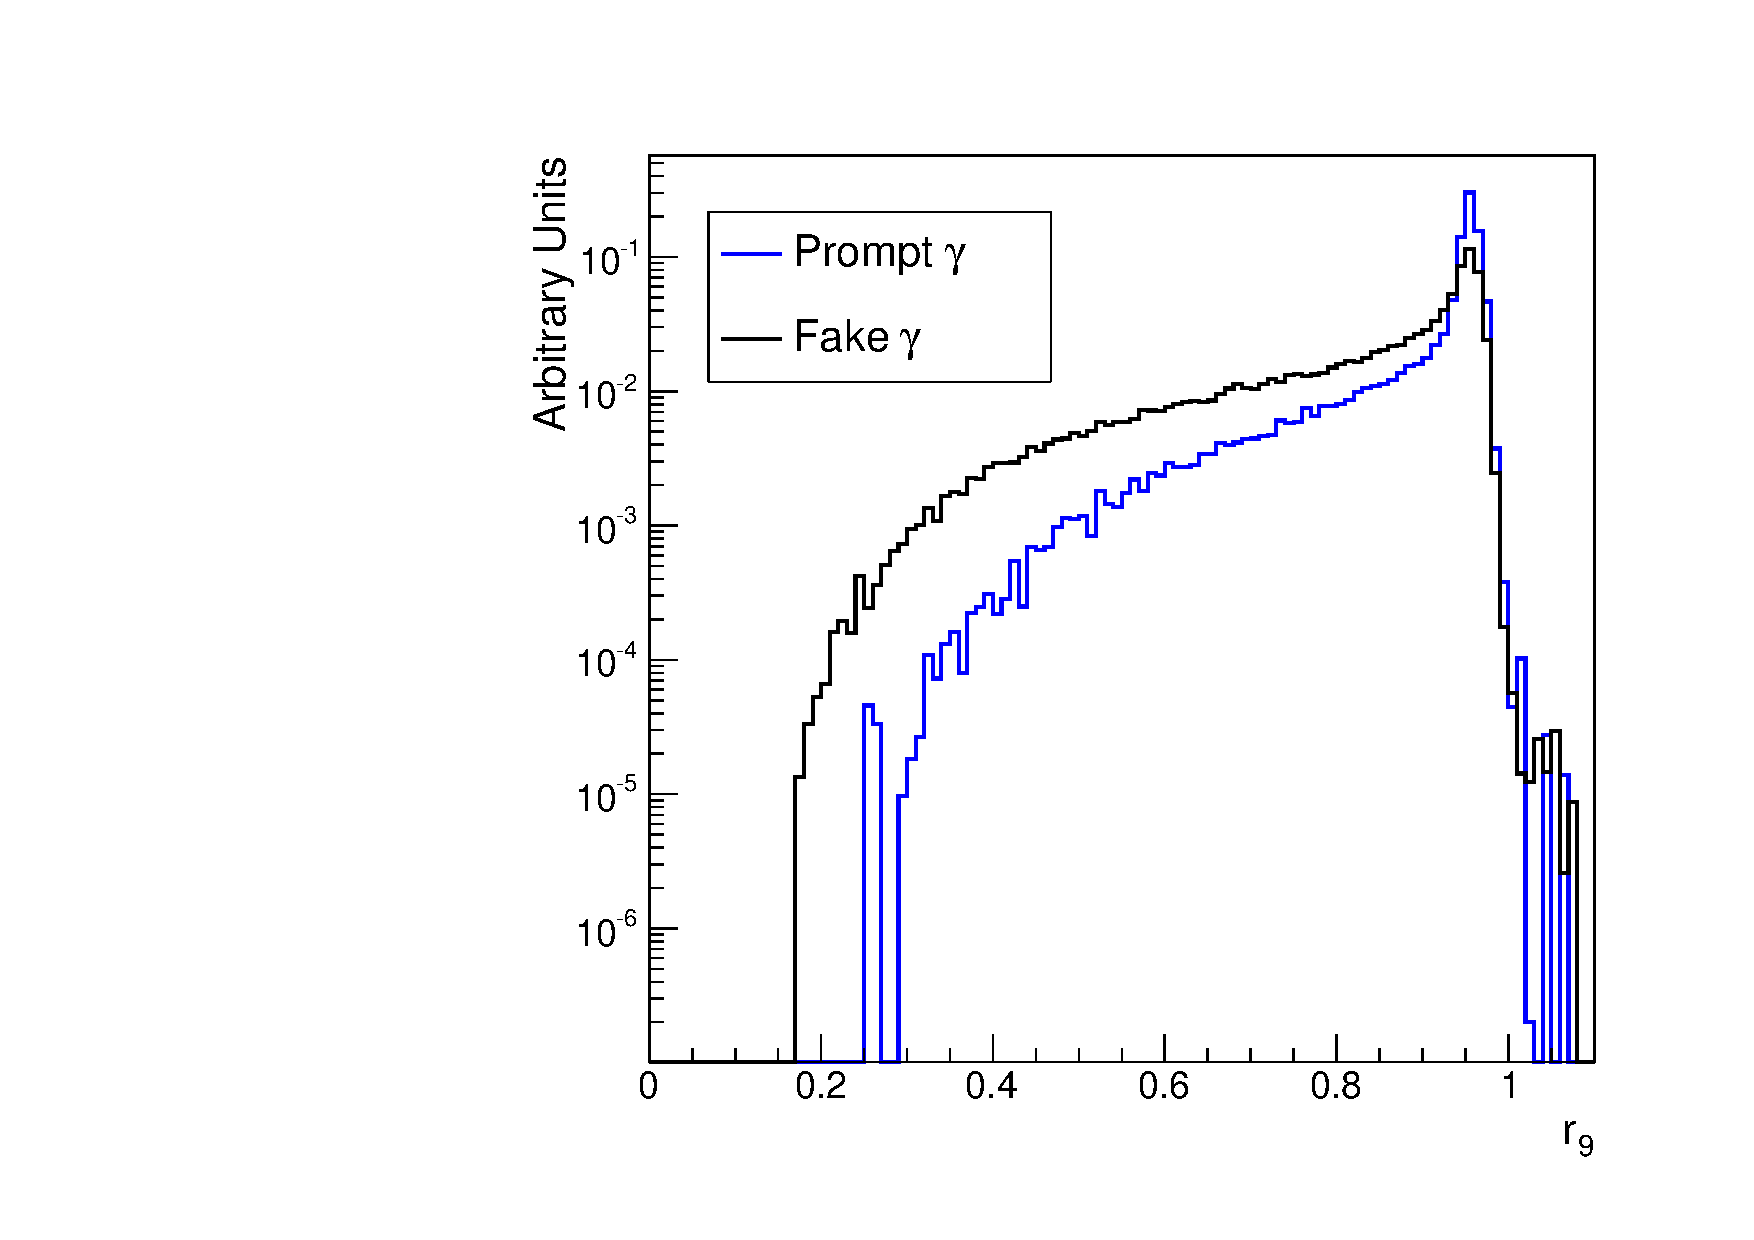
\includegraphics[width=0.49\textwidth]{detector/r9eg.pdf}
	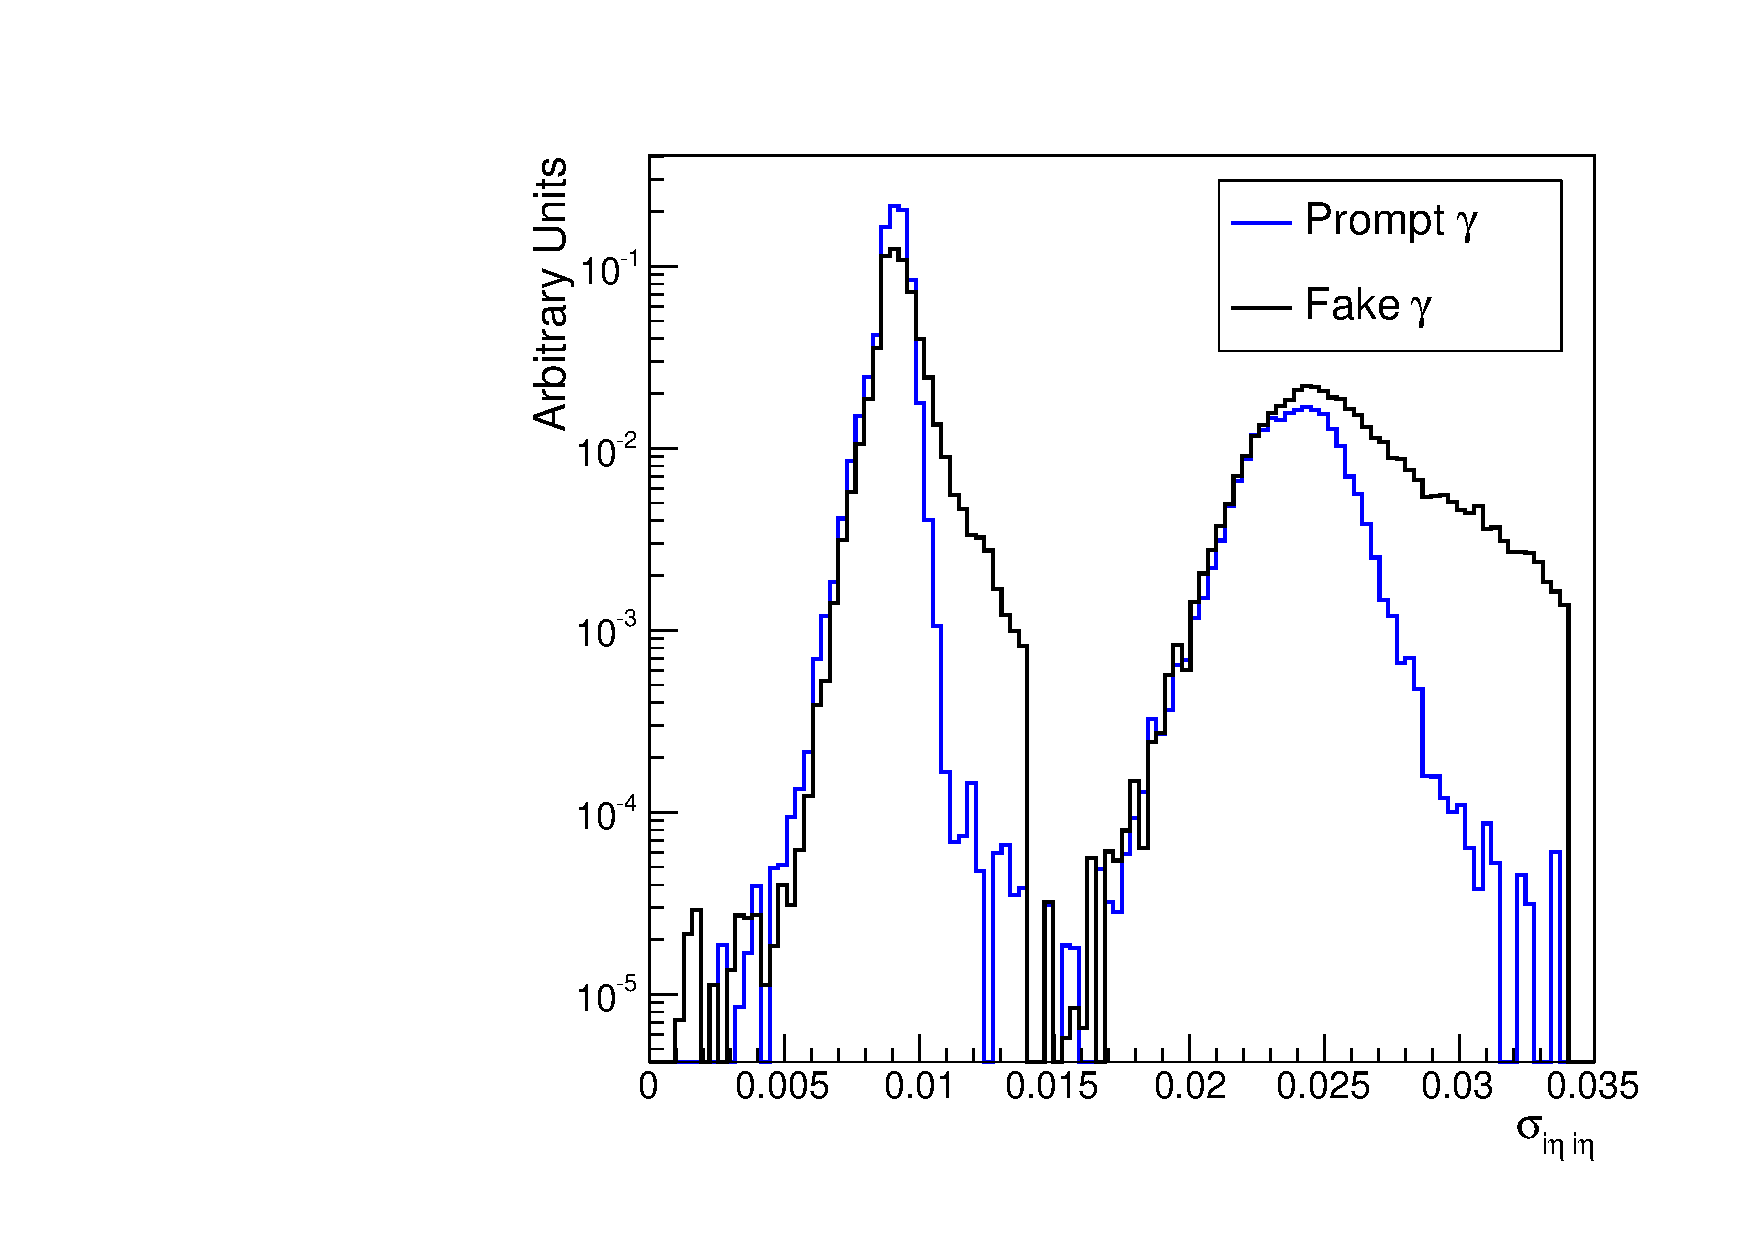
\includegraphics[width=0.49\textwidth]{detector/sieieeg.pdf}
	\caption{Shower shape variable $\rnine$ (left) and $\sigieie$ (right) distributions 
	for superclusters associated with simulated real and fake photons. The real photon is taken
	from simulated $\Hgg$ events while the fake photon is taken from a $\gamma+jet$ sample
	where the photon candidate is matched to a generated quark leg. In the right hand plot,
	two distributions can be distinguished. The narrower is from photons in the barrel and
	the wider from photons in the endcaps. }
	\label{fig:showershape}
\end{center}
\end{figure}

Hard interaction processes tend to produce electromagnetic particles which are well
isolated in the detector. A cone is defined around the candidate with radius $\Delta R$ defined as,
\begin{equation}
\Delta R = \sqrt{(\Delta\phi)^{2}+(\Delta\eta)^{2}}
\end{equation}
where $\Delta\phi$ and $\Delta\eta$ are defined as the $\phi$ and $\eta$ co-ordinates relative to the 
weighted centre of the supercluster.

The sum of $E_{T}$ for each crystal inside the cone, after removing those associated 
to the supercluster itself, quantifies the isolation of the electron or photon candidate.
Similar isolation variables are defined for the HCAL and tracker by
summing over the $E_{T}$ and $p_{T}$ of HCAL deposits and tracks respectively.


\section{Level-1 Trigger}
\label{sec:l1trigger}

In order to cope with the high collision rate, a two-tier trigger
system is implemented at CMS. The trigger is able to use 
limited information from each event to decide whether or not
to record the event. This allows for a large reduction in the rate
of data-taking while maintaining a high efficiency to select events
producing interesting physics objects.
The first level, the Level-1 (L1) trigger, uses custom-built 
electronics in order to reduce the output rate from 40 MHz to 100 kHz~\citep{l1}.
Events which satisfy some relatively loose set of criteria are passed to 
the second level, the high-level trigger (HLT), where more sophisticated
algorithms, much closer to those used in the offline reconstruction,
are used to decide whether or not to store an event~\citep{hlt}.

The L1 calorimeter trigger is able to
use coarse measurements of the energy deposited in the ECAL and HCAL
to form candidate physics objects such as electrons, photons, tau leptons
decaying hadronically and hadronic jets. With the exception of 
electrons and photons, all of the L1 algorithms run in the Global Calorimeter
Trigger (GCT).  The following section is a description of 
a set of calibrations for the GCT designed to improve the resolution of 
the L1 jets.  

\subsection{Jet Energy Calibration}
\label{sec:jetenergyresponse}
The response of the hadronic calorimeter varies
considerably across its barrel, endcap and forward sections. 
The energies of jets are corrected offline to account for these effects,
however, if left uncalibrated at L1, this can lead to inefficiencies in the 
trigger system. The response is measured in QCD Monte Carlo (MC)
simulation by comparing the $p_{T}$ of L1 jet candidates to generated
jets. The generated jets are reconstructed using an anti-$k_{T}$ jet finding algorithm~\citep{antikt}. 
L1 jets are matched
to generator jets by determining the minimum separation, $\Delta R$, between 
each generator jet and any L1 jet candidate and requiring it be less than 0.7.
This is much looser than typical matching requirements applied offline due to the coarser
spatial resolution of the L1 jets.
The generator and the closest of these L1 jet is defined as a matched pair
and the response is calculated as $\Lonept/\Genpt$ for that pair.
Figure~\ref{fig:respvseta} shows the response as a function of the pseudo-rapidity of the
generated jet $|\Geneta|$.

\begin{figure}
\begin{center}
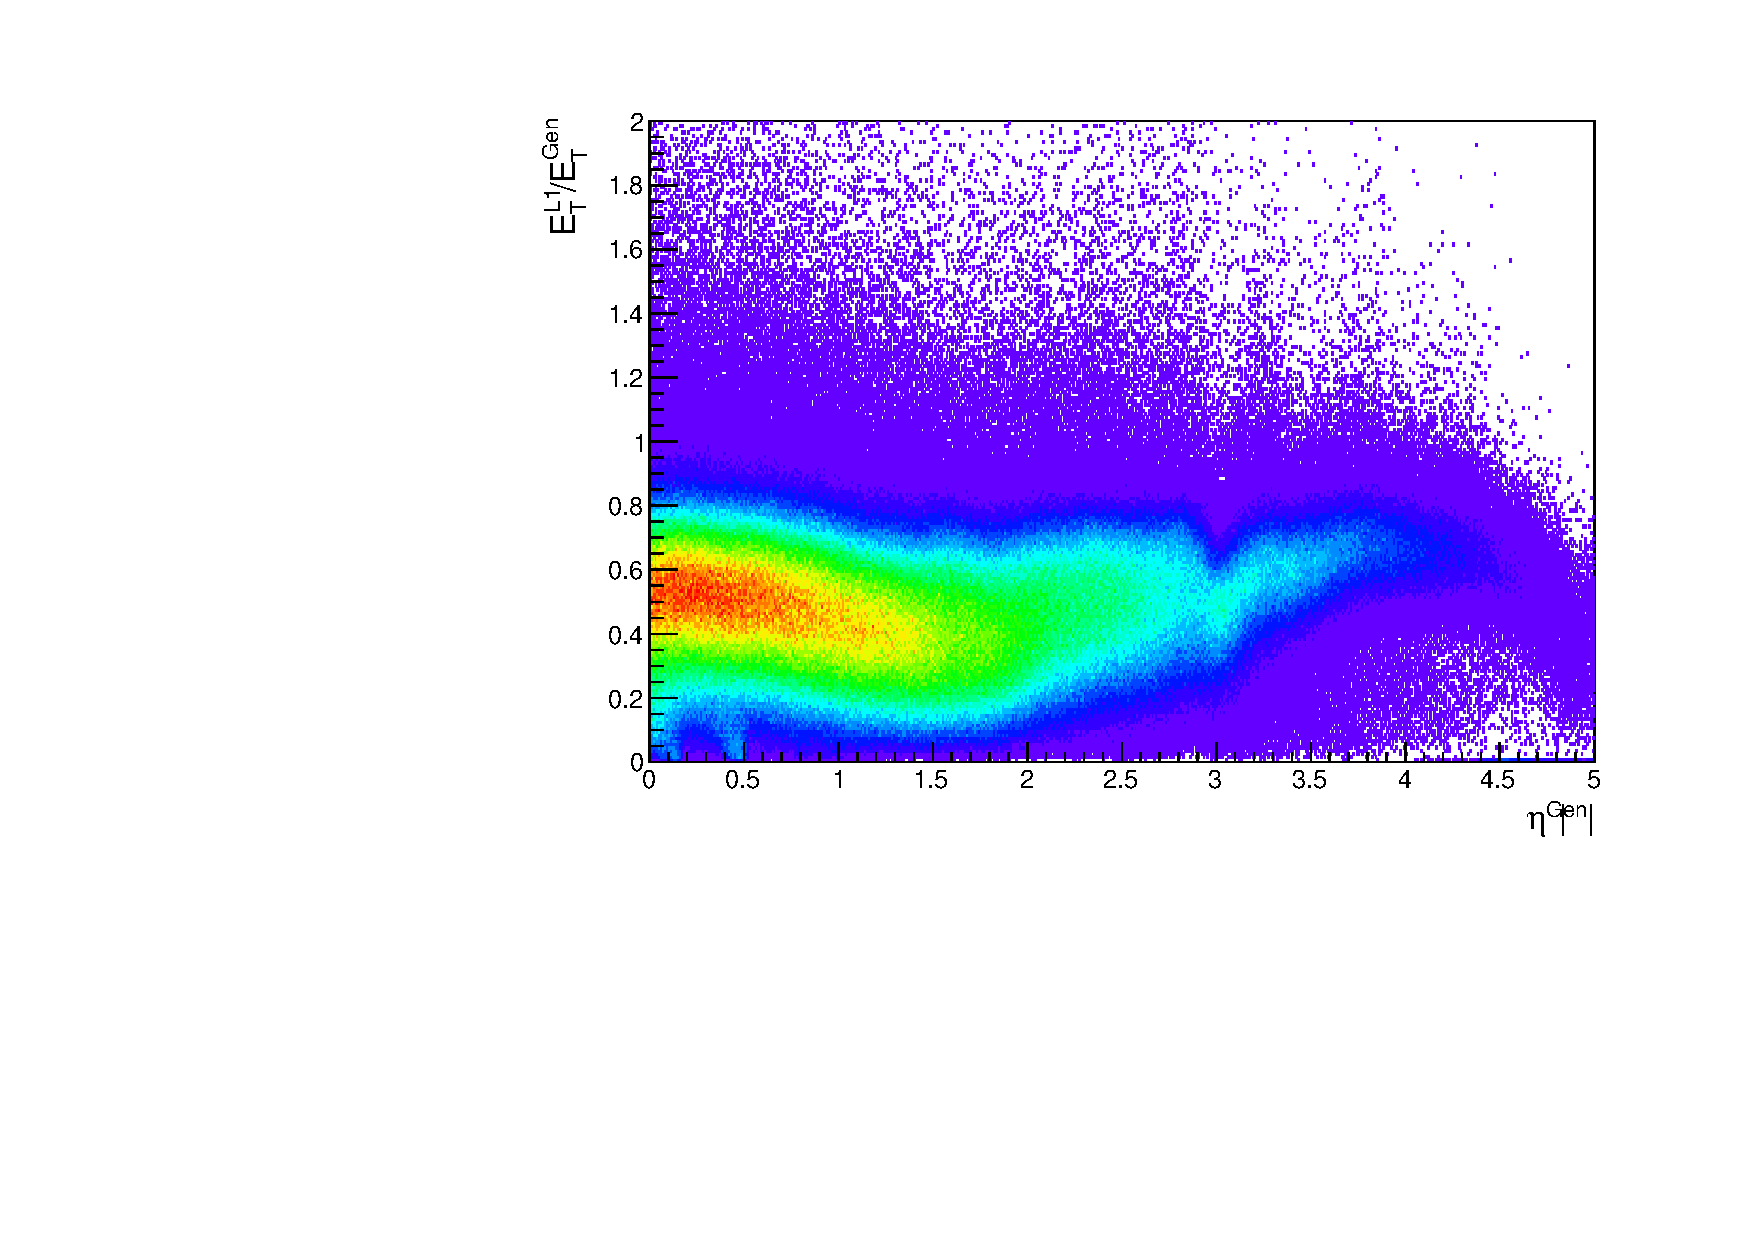
\includegraphics[width=.8\textwidth]{detector/l1jet/bias.pdf}
\caption{Response measured from matched generator-L1 jet pairs in MC 
	as a function of the generator jet pseudo-rapidity $|\Geneta|$.}
\label{fig:respvseta}
\end{center}
\end{figure}

The response is measured in 11 $|\eta|$ bins which correspond to the 11 GCT regions.
Corrections for each region are derived as a function of $\Lonept$ by determining 
the average response, $\left<\Lonept/\Genpt\right>$, and $\left<\Lonept\right>$
in 4 GeV bins of $\Genpt$ between 14 GeV and 200 GeV. Below 14 GeV, the resolution in $\Lonept$ restricts
a proper measurement of the response while above 200 GeV, the response approaches unity.
The average response is taken from the mean of a 
Gaussian fit to the distribution of $\Lonept/\Genpt$ while $<\Lonept>$ is taken as the mean 
average of the $\Lonept$ distribution. For low values of $\Genpt$, the response becomes very non-Gaussian
due to the limited resolution of the L1 trigger, so in this case, the average response is taken
as the mean of the $\Lonept/\Genpt$ distribution. The response is inverted to provide a
corrective scale factor in each region as a function of $\Lonept$. This is then parameterised 
by performing a chi-squared fit of the functional form given in Equation~\ref{eqn:jecfit}.

\begin{equation}
\left<\Lonept/\Genpt\right>^{-1} = \Lonept \cdot \left ( p_{0} + 
\frac{p_{1}}{(\log \Lonept)^{2}+p_{2}}+p_{3} \exp(-p_{4}
(\log \Lonept-p_{5} ) ^{2}) \right )
\label{eqn:jecfit}
\end{equation}

The functional form chosen provides a good description of the shape at low $\Lonept$ in the high $|\eta|$ regions 
and is the same as that used for offline jet calibration at CMS~\citep{jetcalib}.
The parameterisation provides a multiplicative correction to be applied to L1 jets online. 
Figure~\ref{fig:egcorrfunc} is an example of the fit in the $0.348 < |\Geneta| < 0.695$ bin.
The full set of fits in each of the 11 $\Genpt$ bins can be found in Appendix~\ref{app:jecfits}.

\begin{figure}
\begin{center}
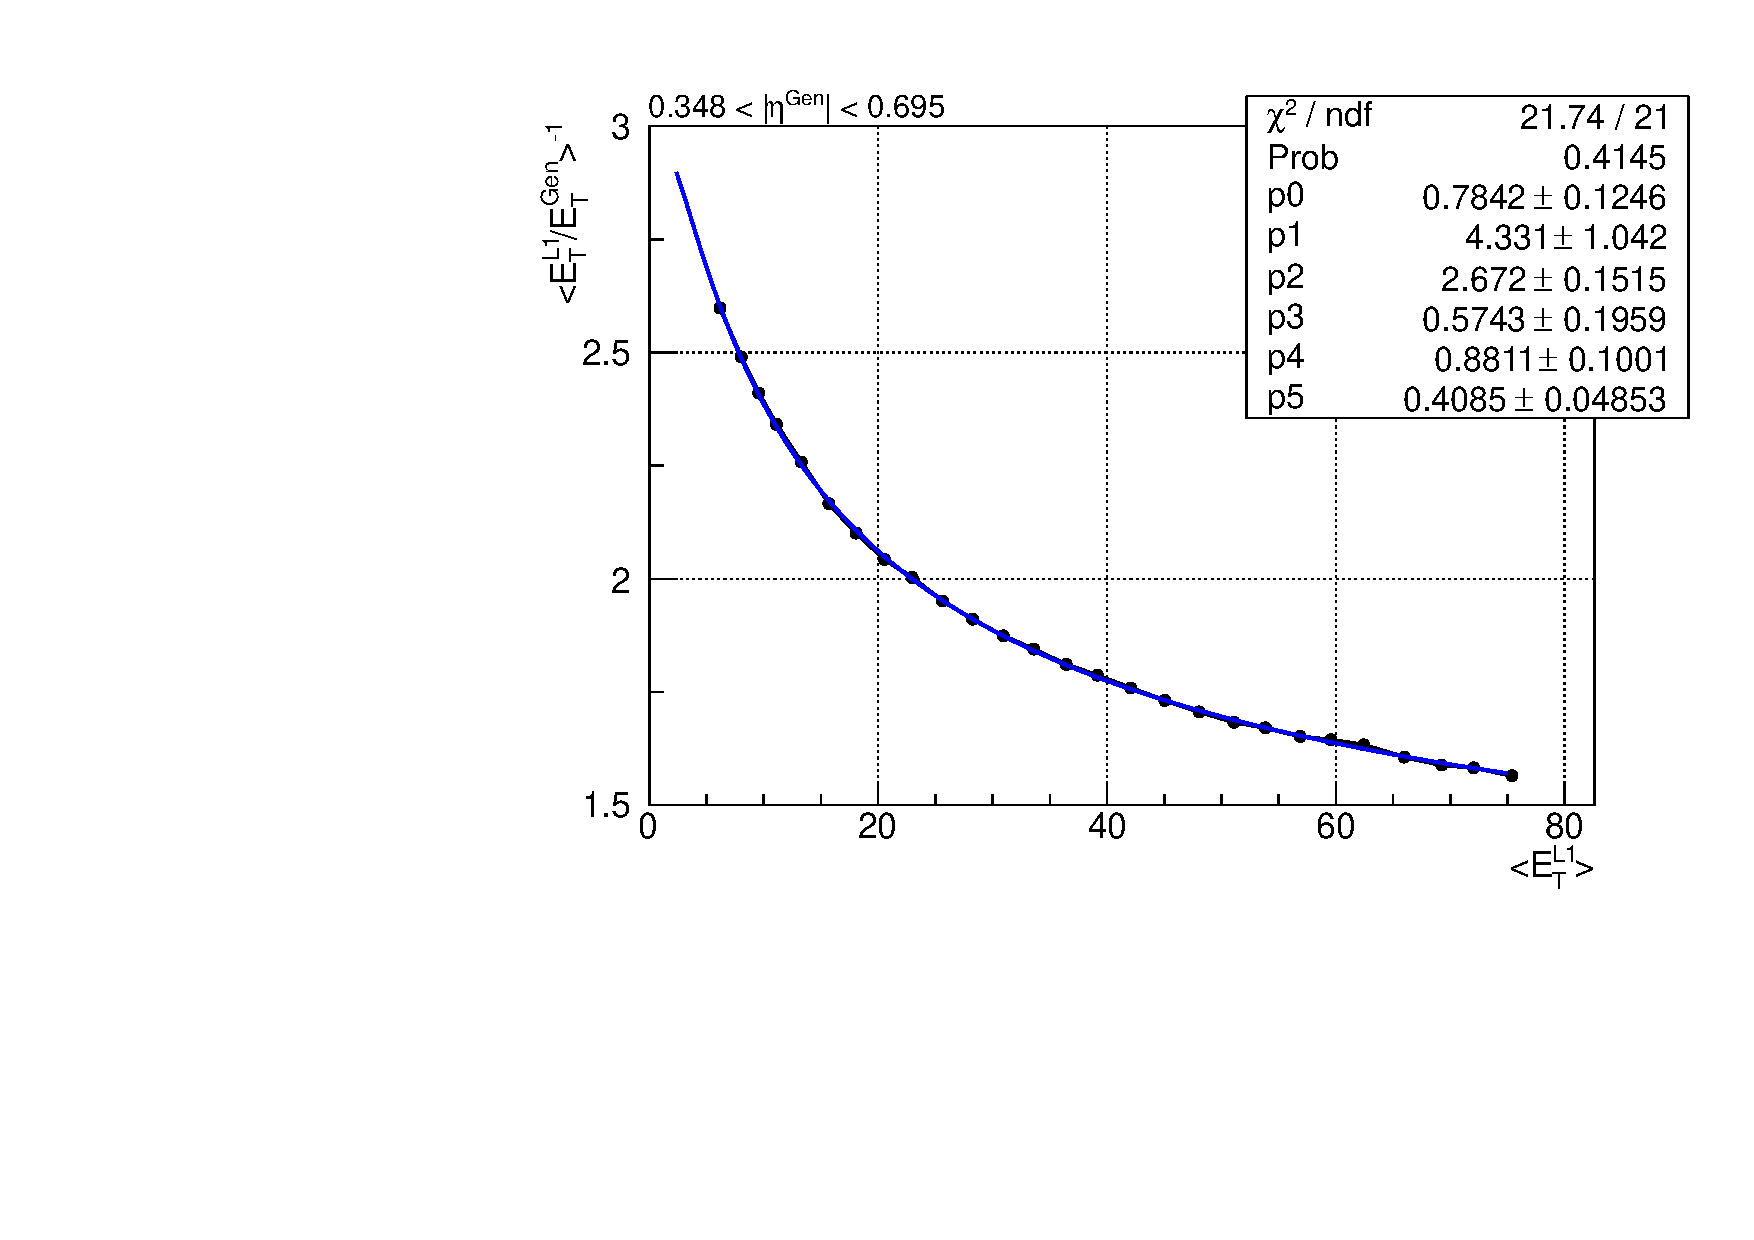
\includegraphics[width=0.8\textwidth]{detector/l1jet/egcorrfunc.pdf}
\end{center}
\caption{Correction function for the $0.348 < |\Geneta| < 0.695$. The points represent the average
quantities as measured in MC. The blue line is a parametric fit to the points 
using a chi-squared minimisation. The error bars, estimated from the number of MC events, are too small 
to be visible in this plot.}
\label{fig:egcorrfunc}
\end{figure}

\subsection{Calibration Performance}
The calibrations derived were applied using the GCT emulation software to the same MC sample 
used to derive them to provide a closure test of their performance. 
The response is shown in Figure~\ref{fig:closure}
as a function of $\Lonept$ and $\Geneta$. The points in each figure are calculated from a Gaussian fit to the distribution
of $\Lonept/\Genpt$ in bins of $\Lonept$ and $\Geneta$ respectively. 
The results show that the procedure closes
to a precision of between 5\% and 10\%. The improvement in L1 jet resolution expected from MC
is demonstrated in Figure~\ref{fig:mcresolutionl1}. The resolution, calculated by fitting a Gaussian to the distribution
of the difference in $E_{T}$ measured at L1 to that of the generator jet 
in bins of $\Lonept$ (see Appendix~\ref{app:closurefits}), for L1 jets is shown before and after applying the
corrections. 
 
\begin{figure}
\begin{center}
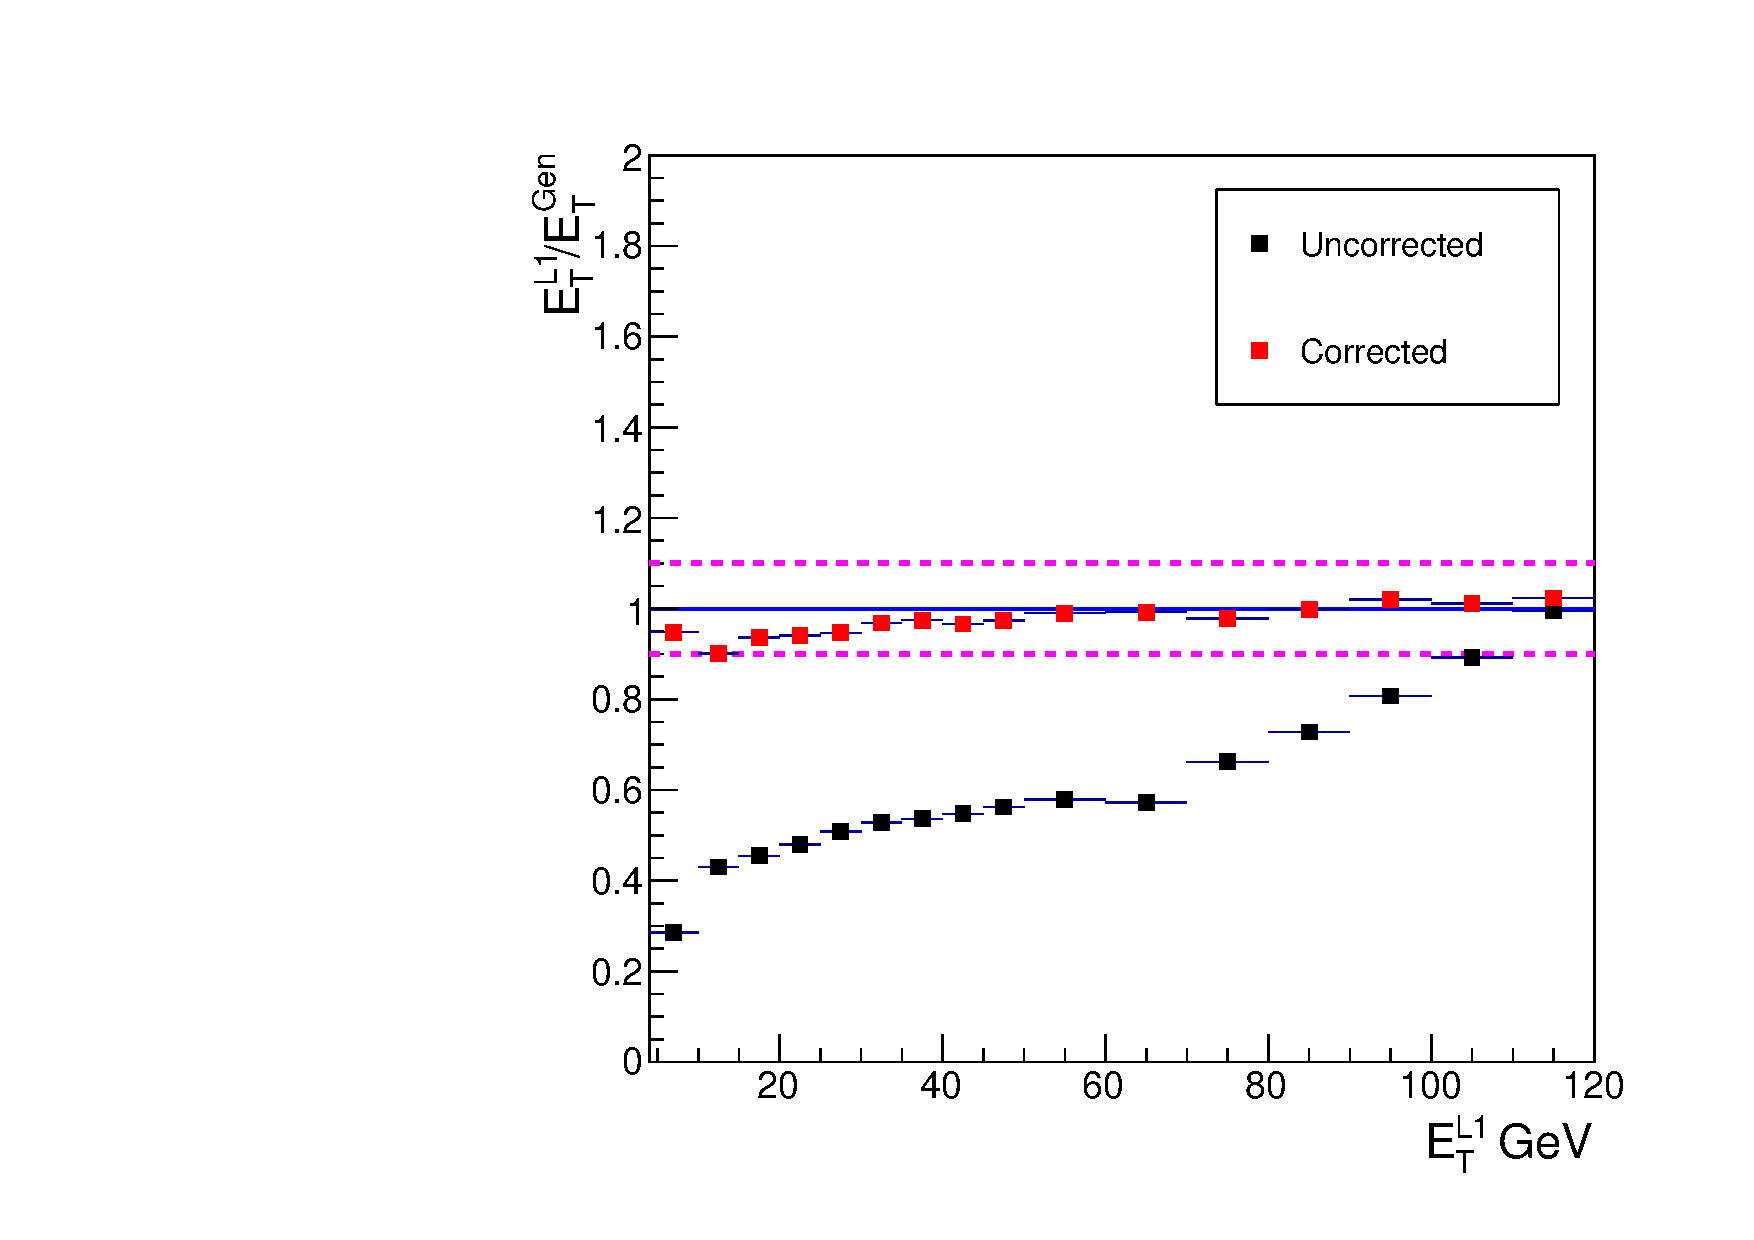
\includegraphics[width=0.49\textwidth]{detector/l1jet/rspvspt.pdf}
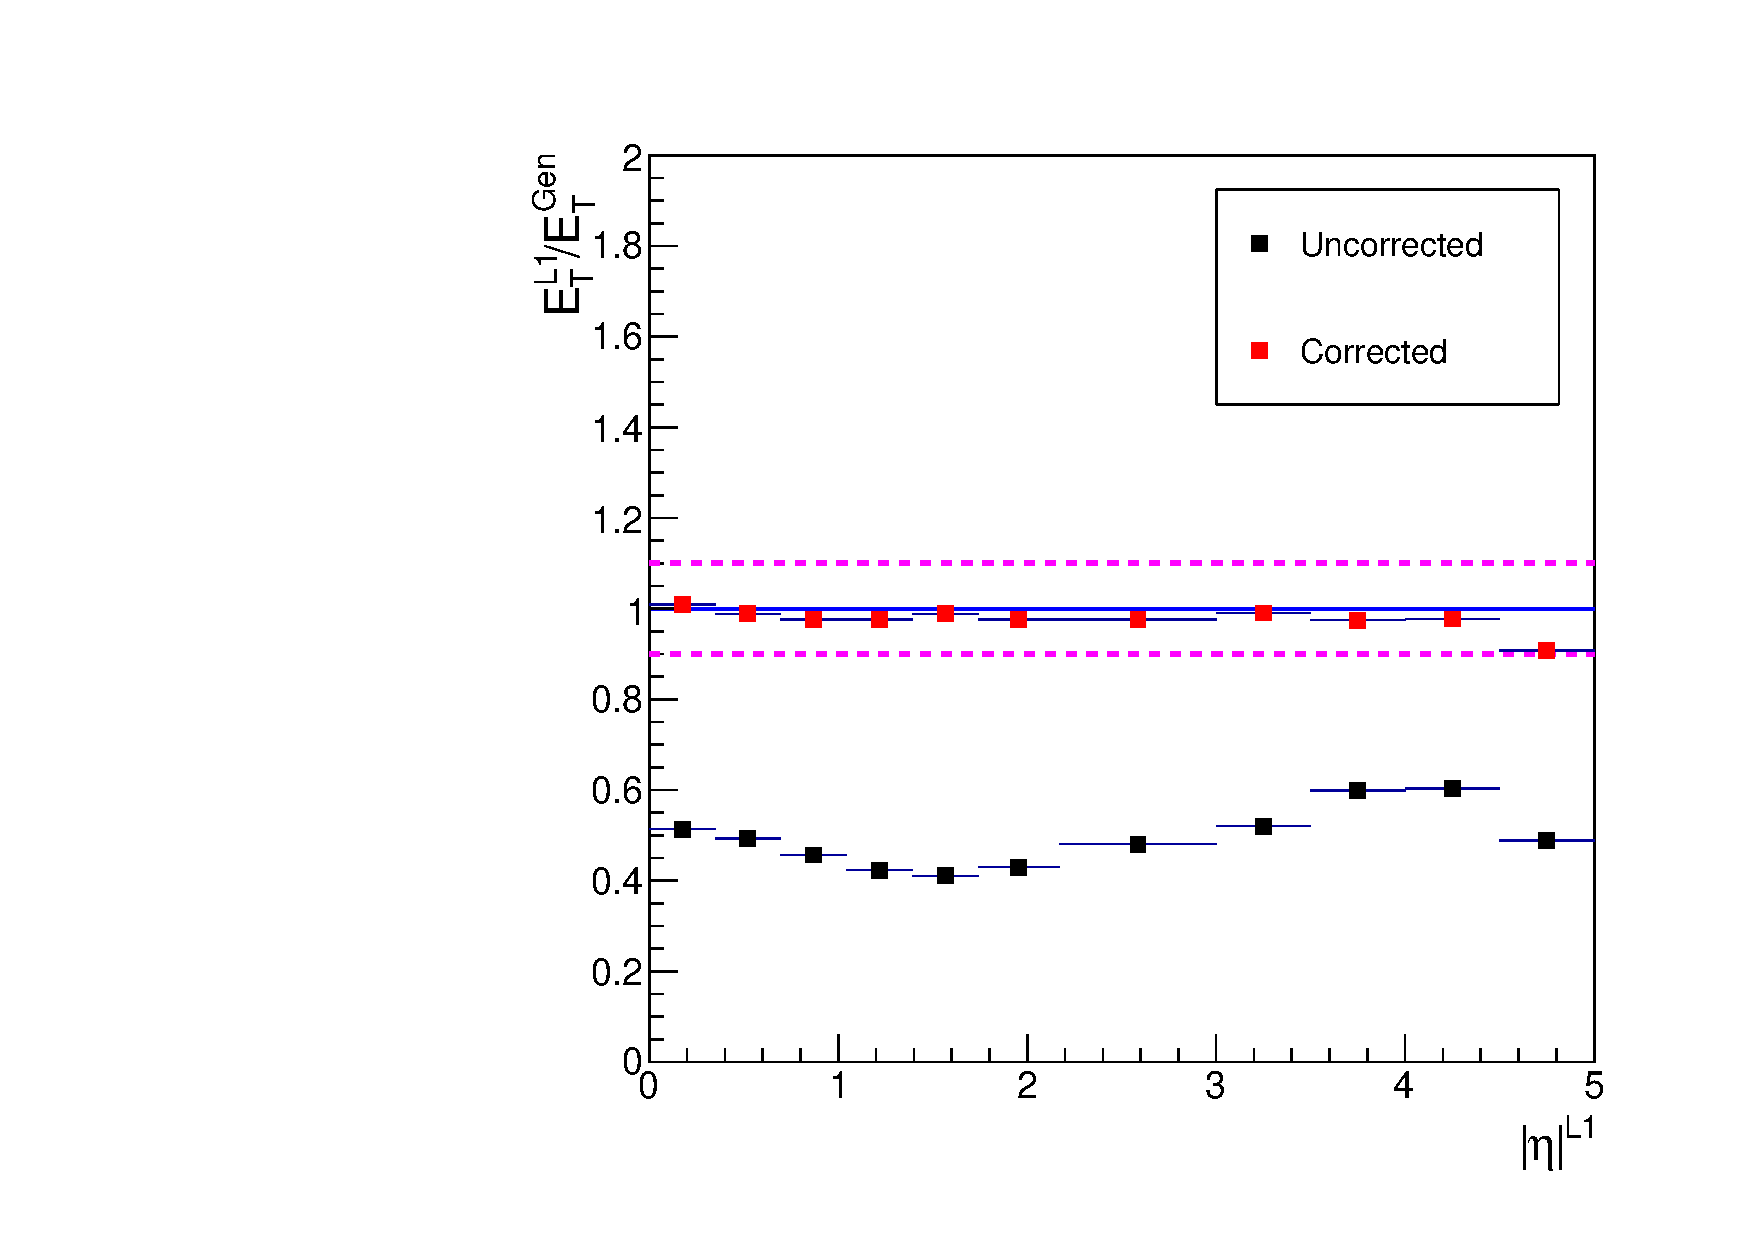
\includegraphics[width=0.49\textwidth]{detector/l1jet/rspvseta.pdf}
\end{center}
\caption{Closure tests performed in MC as a function of $\Lonept$ (left) and $\Geneta$ (right). 
The test shows that after applying the corrections, the response is within 10\% (dashed lines) of unity. 
The error bars are too small to be visible in these plots.}
\label{fig:closure}
\end{figure}

\begin{figure}
\begin{center}
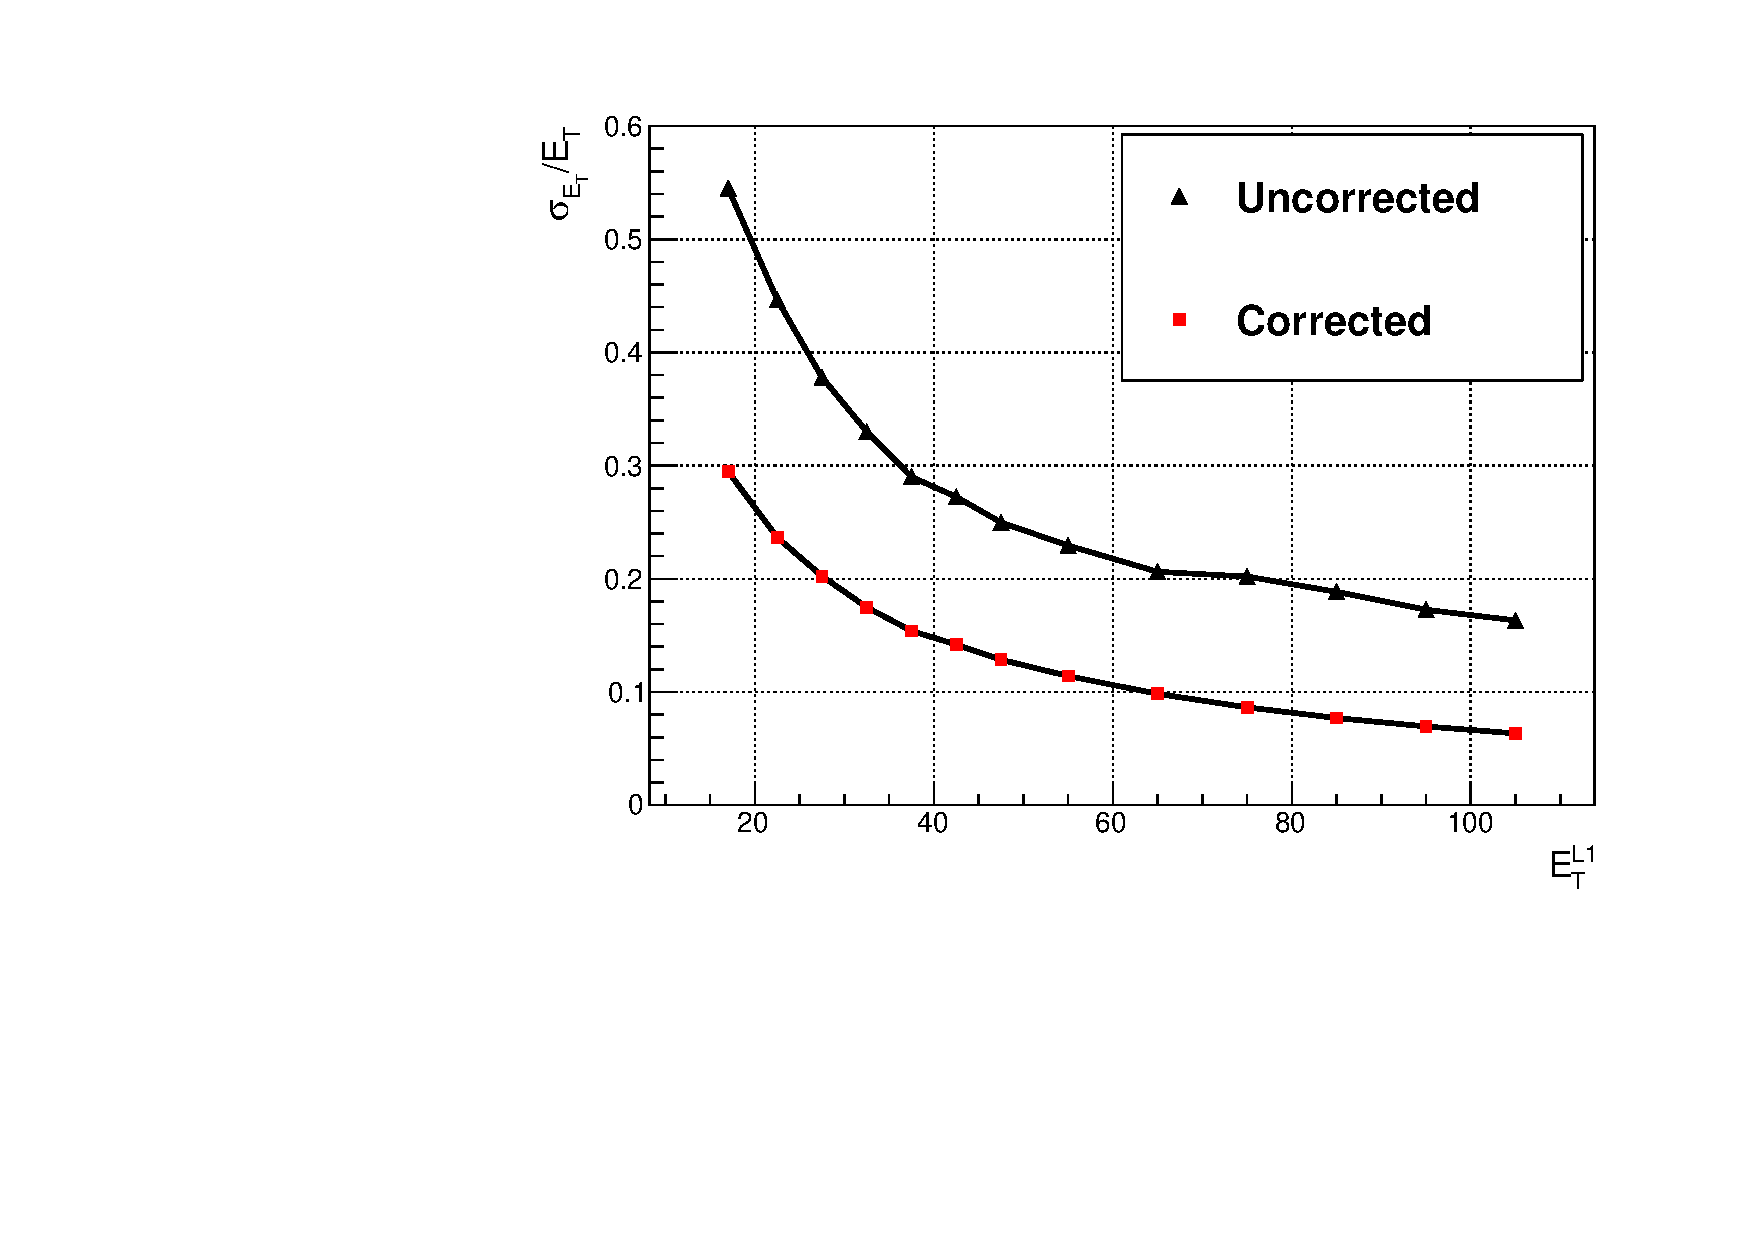
\includegraphics[width=0.8\textwidth]{detector/l1jet/MCresolution.pdf}
\end{center}
\caption{Jet energy resolution at L1 as a function of $\Lonept$ before and after application of the derived calibrations.
 The error bars are too small to be visible in these plots.}
\label{fig:mcresolutionl1}
\end{figure}


\subsubsection{Performance in Data}
The corrections derived in MC were applied to data online during and since run 2011B.
The resolution as a function of $\Lonept$ was measured using events in data from that run period
using the following method.
First, the fraction of L1 jets above some threshold in $\Lonept$ is determined as a function 
of the fully reconstructed jet $E_{T}$ in data.  
This is then fit with an error function of the form, 
\begin{equation}
\mathrm{erf}(x)\propto \int_{0}^{\frac{x-\mu}{\sigma}} e^{-t^{2}}dt,
\end{equation}
to provide a measure of the average energy in the calorimeters 
for jets which just pass the threshold at L1 ($\mu$) and the resolution of those jets ($\sigma$). 
As the full energy reconstruction for jets at CMS is much
more accurate than the value reconstructed at the L1 trigger, the effects of the jet energy resolution
after applying the full jet reconstruction are negligible. This is repeated for different thresholds in $\Lonept$.
Figure~\ref{fig:l1dataresolution} shows the resolution as a function
of $E_{T}$, where the value of $E_{T}$ is taken from the $\mu$ parameter of each fit. 
The uncertainties on each point represent the statistical uncertainty from the error function fits.
The points are fit with the parameterisation given in Equation~\ref{eqn:resofit} to extract the parameters which describe the
resolution of the calorimeter. The energy resolution of the L1 jets is improved after applying these 
calibrations in the GCT~\citep{l1triggernote}.
%An independent set of corrections were derived and applied during Run2011A but 
%were found to give worse performance than the ones described here in particular for jets with 
%$E_{T}>130$ GeV. 

\begin{figure}
\begin{center}
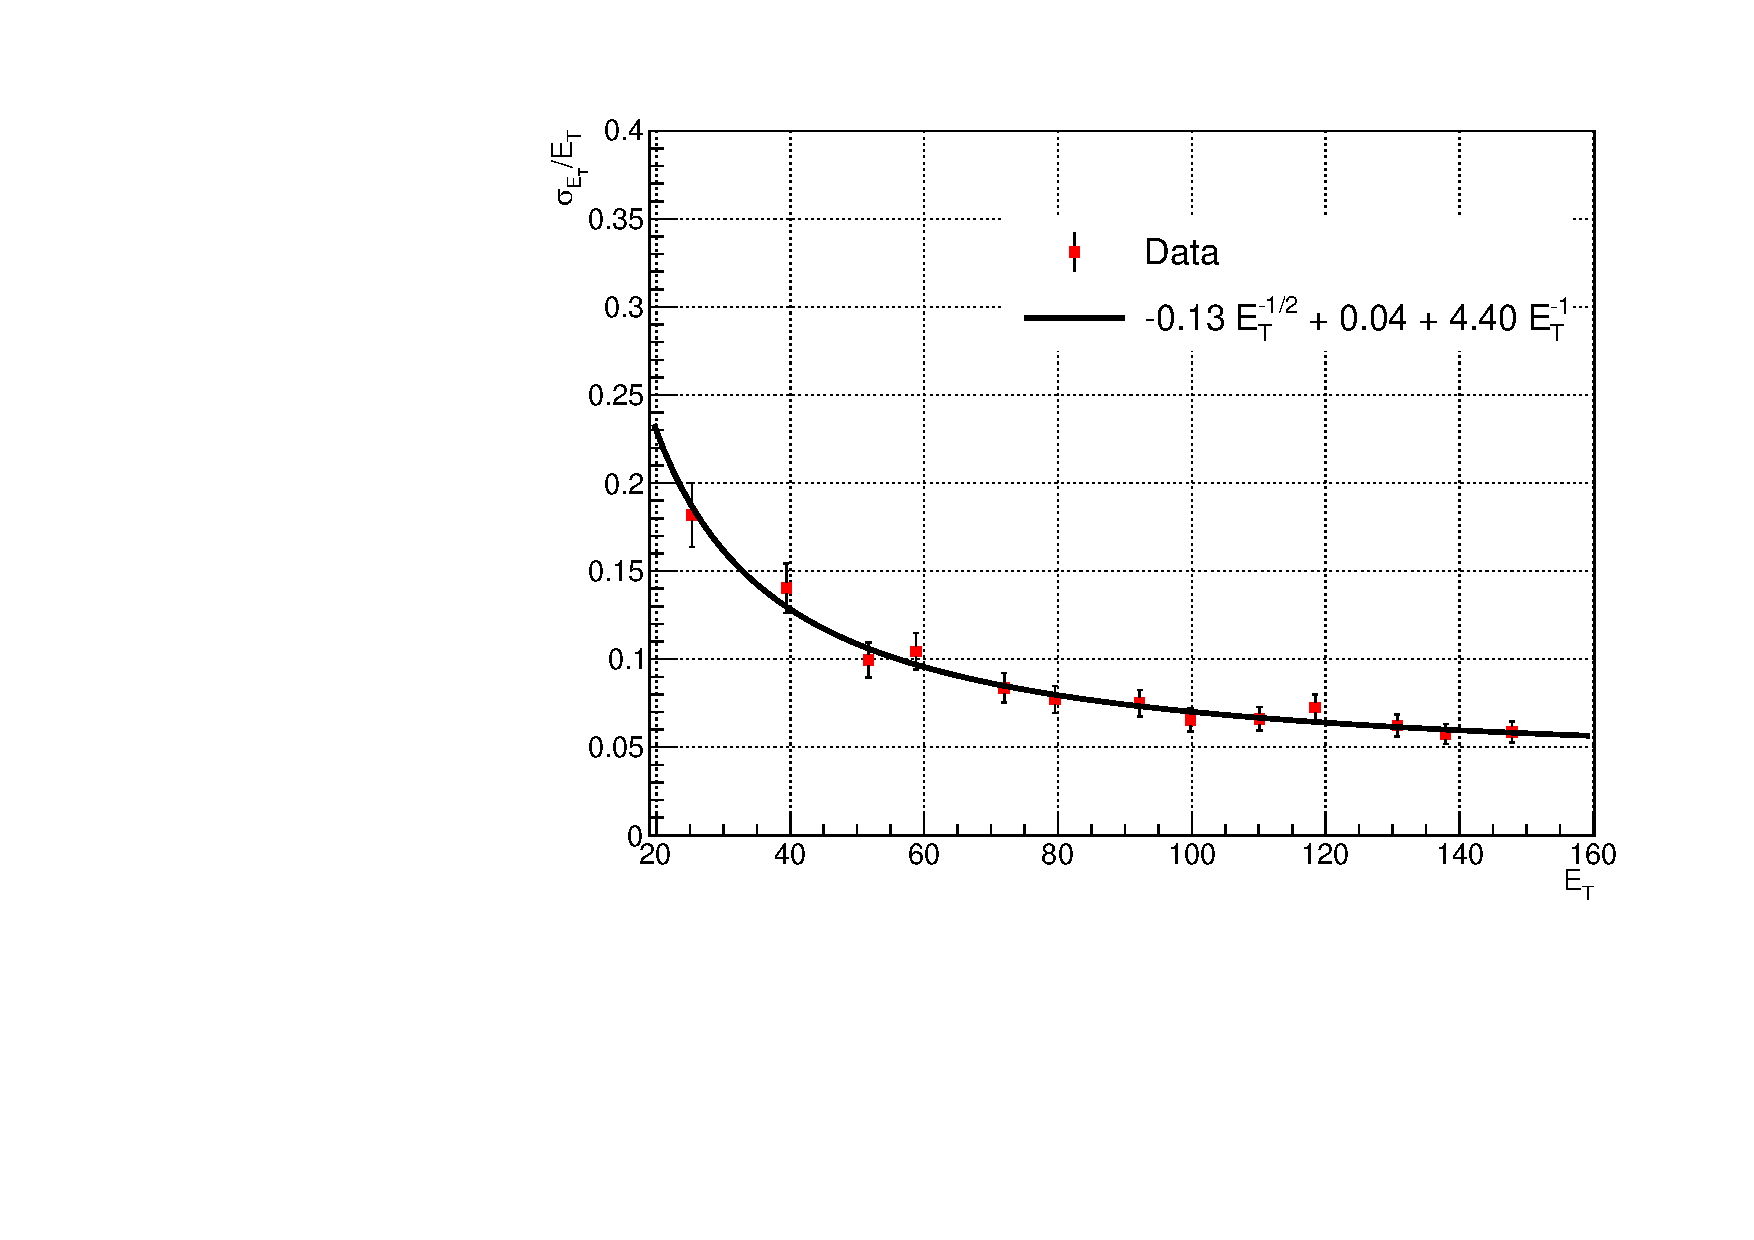
\includegraphics[width=0.8\textwidth]{detector/l1jet/DataResolution.pdf}
\end{center}
\caption{Energy resolution, $\sigma_{E}$, of L1 jets as a function of transverse energy deposited in the
calorimeter, $E_{T}$. The coefficients of the functional form shown are the result of a fit to the points.}
\label{fig:l1dataresolution}
\end{figure}




\chapter{Higgs Decay to Two Photons}
\label{chap:hgg}

The two photon channel is one of the most promising decay modes in the search for the SM Higgs
at the LHC. Despite having a relatively small branching ratio, the decay $\Hgg$ 
provides a very clean, fully reconstructible final-state topology making it 
one of the most sensitive channels at low mass.
The dominant source of background is from real, prompt diphoton events from QCD 
processes, $pp\rightarrow\gamma\gamma$ (prompt-prompt).
In addition, there is a contribution from $pp\rightarrow\gamma+jet$ (prompt-fake) and 
$pp\rightarrow jet+jet$ (fake-fake) in which jets are mis-identified as photons. 
As the signal rate in the $\Hgg$ decay is expected to be small compared to the background rates,
the search sensitivity is heavily influenced by how well the backgrounds are understood.
For this reason, two data-driven background modelling techniques were developed
The first uses a fully parametric
description of the background from data designed to incorporate systematic uncertainties as additional degrees of 
freedom in its functional form~\cite{HIG-11-033}. The second uses a binned model constructed from 
sidebands in the $\mgg$ spectrum. The latter of these two serves as an independent cross-check of the former,
in particular by allowing direct inclusion of the systematic uncertainties in the signal extraction thereby
building confidence in the understanding of the background. 
This chapter describes a search for a Higgs boson decaying to two photons
which was performed on the full 2011 dataset corresponding to \clumi of proton-proton collisions 
recorded at CMS at a center of mass energy of 7 TeV.

\section{Data Samples}
\label{sec:datasamples}

The dataset used for this analysis is the combination of the 2011A and 2011B 
proton-proton collision runs.
The selection for the dataset used for this analysis is based around dedicated diphoton triggers
which select events online which satisfy one of two sets of criteria.
The first set requires two HLT photon candidates, one with $\pt>26$ GeV and the other with 
$\pt>18$ GeV, which are well isolated in the calorimeter~\cite{AN-12-048}. The second has a lower threshold on
the first photon, $\pt>22$ GeV but requires that both photons have localised showers in the ECAL 
($\rnine>0.8$ in 2011A and $\rnine>0.9$ in 2011B). 
Additionally, the invariant mass of the two trigger objects are required to have an 
invariant mass greater than 60 (70) GeV in the 2011A(B) datasets.
Events which would pass the full offline selection but failed to trigger at the HLT lead to an inefficiency, 
reducing the number of signal events with respect to that expected from an integrated luminosity of \clumi.
However, the thresholds applied offline are chosen to be much tighter than those of the trigger;
the trigger efficiency is $>$99\% with respect to the analysis selection~\cite{AN-12-048}. 

Signal Monte Carlo (MC) events are generated for a Higgs decaying to two photons via the four main 
production processes, gluon-gluon fusion ($ggH$), vector boson fusion ($qqH$) and associated $W/Z$ ($VH$) 
and $\ttbar$ ($ttH$) production.
The gluon-gluon fusion and vector boson fusion were generated with \texttt{POWHEG}~\cite{powheg} with 
next-to leading order (NLO) contributions whereas
the two associated production processes were generated to leading order (LO) only.
The $\pt$ spectrum of the Higgs ($\pt^{H}$) from gluon-gluon fusion was calculated at
next-to-next-to leading plus next-to leading log resummed order (NNLO+NLL) using the \texttt{HqT} program~\cite{hqt}.
The production cross-sections and branching ratios are taken from the LHC Cross-section Working Group~\cite{lhcxswg}.

MC for background processes were generated at LO using \texttt{POWHEG} interfaced with \texttt{PYTHIA}~\cite{pythia}.
The QCD dijet and $\gamma+jet$ samples are filtered by requiring the generated photons, electrons and neutral
mesons with $\pt>15$ GeV have at most one charged particle in a cone, $\Delta R<0.2$, to increase the 
production efficiency with respect to the tracker isolation requirements of the full selection.
The background samples considered for this analysis are summarized in Table~\ref{tab:backgroundmc}.
A full simulation of the CMS detector is provided in \texttt{GEANT4} which is used for all signal
and background MC samples~\cite{geant4}. The MC includes a simulation of additional interaction vertices expected in data
from pileup. The distribution in the number of reconstructed vertices in MC  is corrected to match that observed
in data as described in Section~\ref{sec:pileup}.

\begin{table}
\begin{center}
\begin{tabular}{|l r|c|c|}
\hline
\textbf{Process}  & &  \textbf{Cross-section} ($pb$) & \textbf{Luminosity} ($pb^{-1}$)\\
\hline
\hline
DiPhotonJets & & 154.7 & 7400 \\
\hline
DiPhoton Box & $\hat{\pt}~25-250$ & 12.37 & 41900 \\
\hline 
QCD Dijet    & $\hat{\pt}~30-40$      & 10870 & 560 \\
	     & $\hat{\pt}~40-\infty$  & 43571 & 920 \\
\hline 
Gamma+Jet    & $\hat{\pt}~20-\infty$  & 493.44& 2400 \\
\hline 
DrellYan+Jets to $ll$  & $\hat{\pt}~50-\infty$  & 2475& 14000 \\
\hline
\end{tabular}
\caption{Background MC used throughput the analysis with production cross-sections and 
corresponding equivalent integrated luminosity.}
\label{tab:backgroundmc}
\end{center}
\end{table}


\section{Object Reconstruction and Identification}
\label{sec:objectrecoandid}

The reconstruction of all objects used for this analysis, in both data and MC,
is based on the standardized CMS reconstruction software \texttt{\cmssw}~\cite{null}. 
Additional sensitivity can be gained by refining the object selection and reconstruction specifically
to the search for $\Hgg$.

\subsection{Supercluster Energy Correction}
\label{sec:superclusterenergyreconstruction}

As the natural width of Higgs boson is around 100 MeV, the width of a reconstructed mass peak from 
a $\Hgg$ decay is driven by the experimental energy resolution of the photons.
This resolution can be improved dramatically by correcting the raw energy of the supercluster 
on a per-photon level. These corrections are derived using a multivariate technique 
in which a regression BDT is trained on prompt photons in the gamma+jet MC sample using the 
ratio of the generated photon energy to the raw energy of the reconstructed supercluster.
As this ratio can vary across different regions of the detector, the input variables include both the 
$\eta$ and $\phi$ positions of the supercluster. In addition, several variables are included which 
describe the shower shape: $\rnine$, the energy weighted widths in $\eta$ and $\phi$ of the supercluster,
the energy weighted crystal width ($\sigieie$) and the ratio of hadronic energy behind the supercluster
to the energy of the supercluster itself ($\hoe$). In the endcaps, there is additional information 
available from the pre-shower measurement. The ratio of the energy in the pre-shower to the raw supercluster energy
is included for superclusters in the ECAL endcaps. Figure~\ref{fig:mcregrcomparison} shows the improvement
in resolution after applying the regression corrections compared to the raw measurement.
In addition, a similar set of corrections were derived using by fitting an analytical expression 
of the residual energy difference between the 
generated and reconstructed photon energy as a funciton of supercluster energy, position and $\rnine$~\cite{AN-11-343}. 
The regression technique reduces the effective resolution of the Higgs mass peak ($\sigma_{eff}$) 
resolution by around 30\% over using the raw supercluster energy compared to the analytic fit which
improves the resolution by 15\%. 

\begin{figure}
\begin{center}
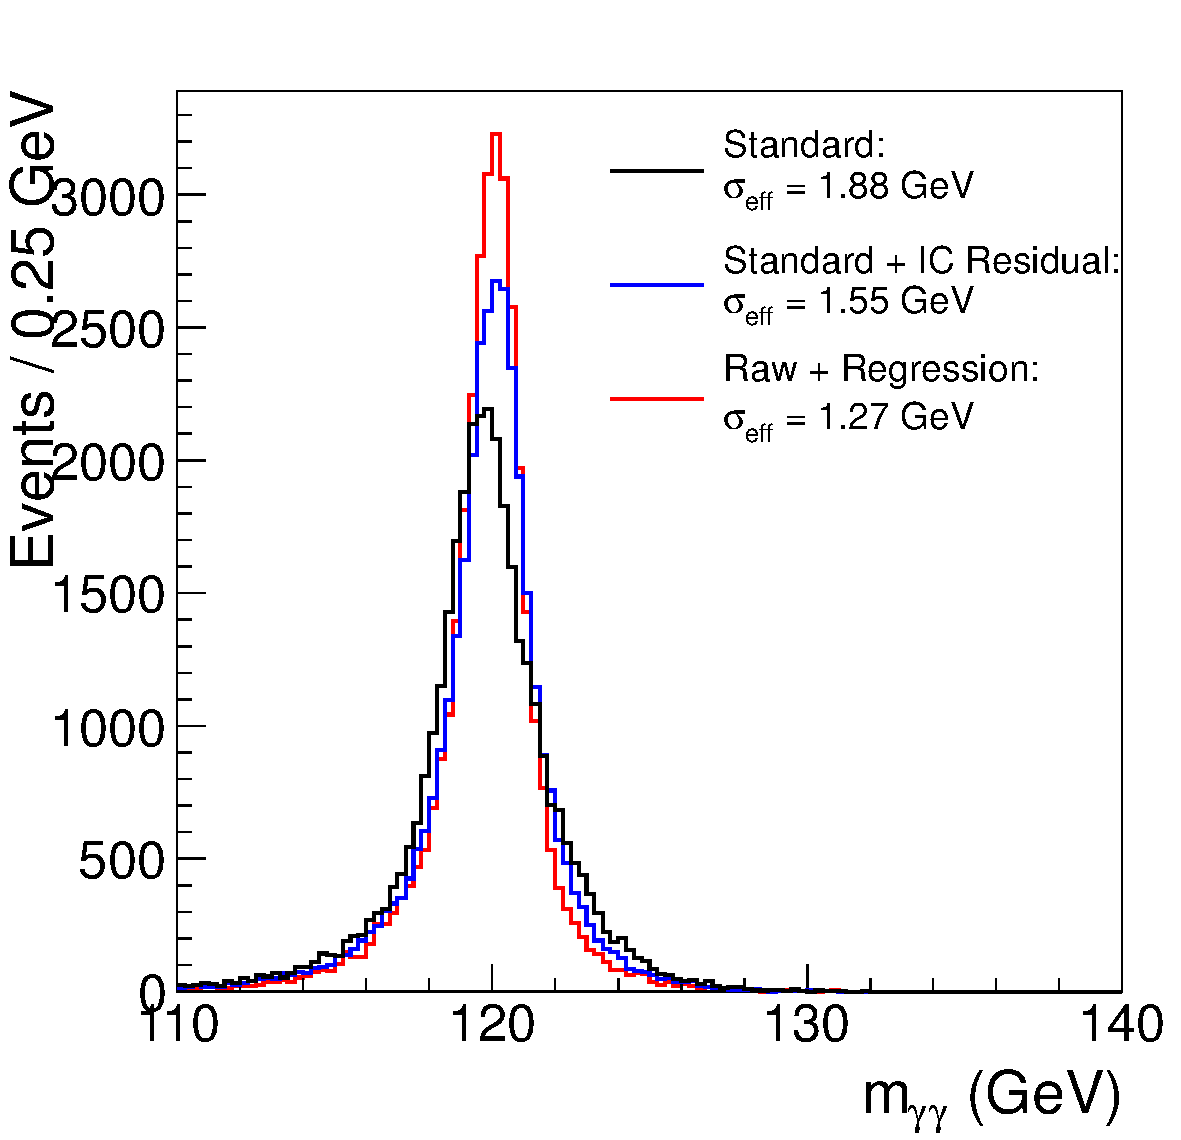
\includegraphics[width=.6\textwidth]{hgg7TeV/generalPlots/regrresall.pdf}
\label{fig:mcregrcomparison}
\caption{Comparison of the diphoton mass peak in MC Higgs with a mass of 120 GeV using different 
measurements of the photon energy. The black line 
is from using the raw energy of the supercluster, the blue is from using the analytic fit method 
and the red from using the regresssion method. The quantity $\sigma_{eff}$,
the narrowest range in $\mgg$ which contains 68\% of the distribution, is given for each peak.}
\end{center}
\end{figure}

An estimate of the per-photon energy resolution, $\sigma_{E}$, is obtained by training a second 
regression BDT targeting the absolute deviation between the correction estimated by the 
first BDT and the true correction to generator level. This second BDT is trained on an independent
set of events to the first. The per-photon resolution is used to calculated an estimate of the 
per-event mass resolution, $\sigma_{\mgg}$, which is used during the event selection 
(Section~\ref{sec:eventselection}). An additional regression BDT is trained on $\Zee$ MC which is used
to compare the supercluster energy scale in data and MC~\cite{AN-12-048}.

\subsubsection{Energy Scale Measured in Data}
Despite correcting the energy of the photons using the regression technique, discrepancies between data and
MC are still observed. This is due to additional detector effects which may not be simulated, such as the
time dependence of the ECAL crystal transparency~\cite{null}. Further corrections are
derived based on $\Zee$ events which provide an invariant mass peak with almost no background constructed from 
electromagnetic objects which are reconstructed using a similar procedure to photons.
The energy scale of the superclusters is measured by matching the electron
invariant mass peak in data to that in MC. This is achieved using an analytic fit to the $\Zee$ peak in data and MC
separately. The natural peak of the $Z$ is described using a Breit-Wigner distribution whose parameters are fixed
to those given by the Particle Data Group, $m_{Z}=91.188,~\Gamma_{Z} = 2.495$~\cite{pdg}. This is then convoluted 
with a Crystal Ball (CB) which describes the resolution effects of the calorimeter and energy losses from 
bremsstrahlung before the ECAL~\cite{crystalball}. 
The CB parameter $\Delta m$ is a free parameter of the fit giving the 
offset of the peak position from the $Z$ pole. 

The values of these fitted parameters varies with the position of the supercluster ($|\eta|$). Moreover the
variation in data is strongly dependant on the run during which the data were taken. The scale is extracted in 
six run ranges and four $|\eta|$ regions to account for this effect. 
The difference between MC and data with time is less dependant on whether the electron showered or not which 
is characterised by the $\rnine$ of the supercluster. The data-MC difference in each $|\eta|$ region is measured
a second time after applying the first set of corrections to the data and obtaining the residual difference
for electrons with $\rnine<0.94$ and $\rnine>0.94$ separately. The final energy scale correction is then defined
as the product of the two corrections. The relative correction, 

\begin{equation}
1-\Delta P = 1 - \frac {\displaystyle \Delta m_{data} - \Delta m_{MC} }{\displaystyle m_{Z} }
\end{equation}

is applied to the photons in data. The values for the scale in each category, $\Delta P$, are given in 
Table~\ref{tab:escale2011}. The uncertainties on these measurements are primarily due to 
the difference in the $\rnine$ distribution of electrons and photons. In addition, smaller systematics
are included due to the variation of the measurements when changing the electron selection and
between using the electron-trained and photon-trained regression corrections.
These uncertainties are incorporated into the signal model for the purposes of 
signal extraction as described in Section~\ref{sec:signalmodel}.

\subsection{Vertex Selection}
\label{sec:vertexselection}

The assignment of the correct vertex to the diphoton pair is an important step in the reconstruction of 
its invariant mass. Since photons do not leave tracks, computing the angle between the two photons 
depends strongly on determining the interaction in which they were produced.
Figure~\ref{fig:higgsrightwrongvertex} shows the invariant mass distributions from a SM
Higgs boson for events in which the vertex selected is within 10mm of the generated vertex
compared to those in which an incorrect vertex is assigned. 

\begin{figure}
\begin{center}
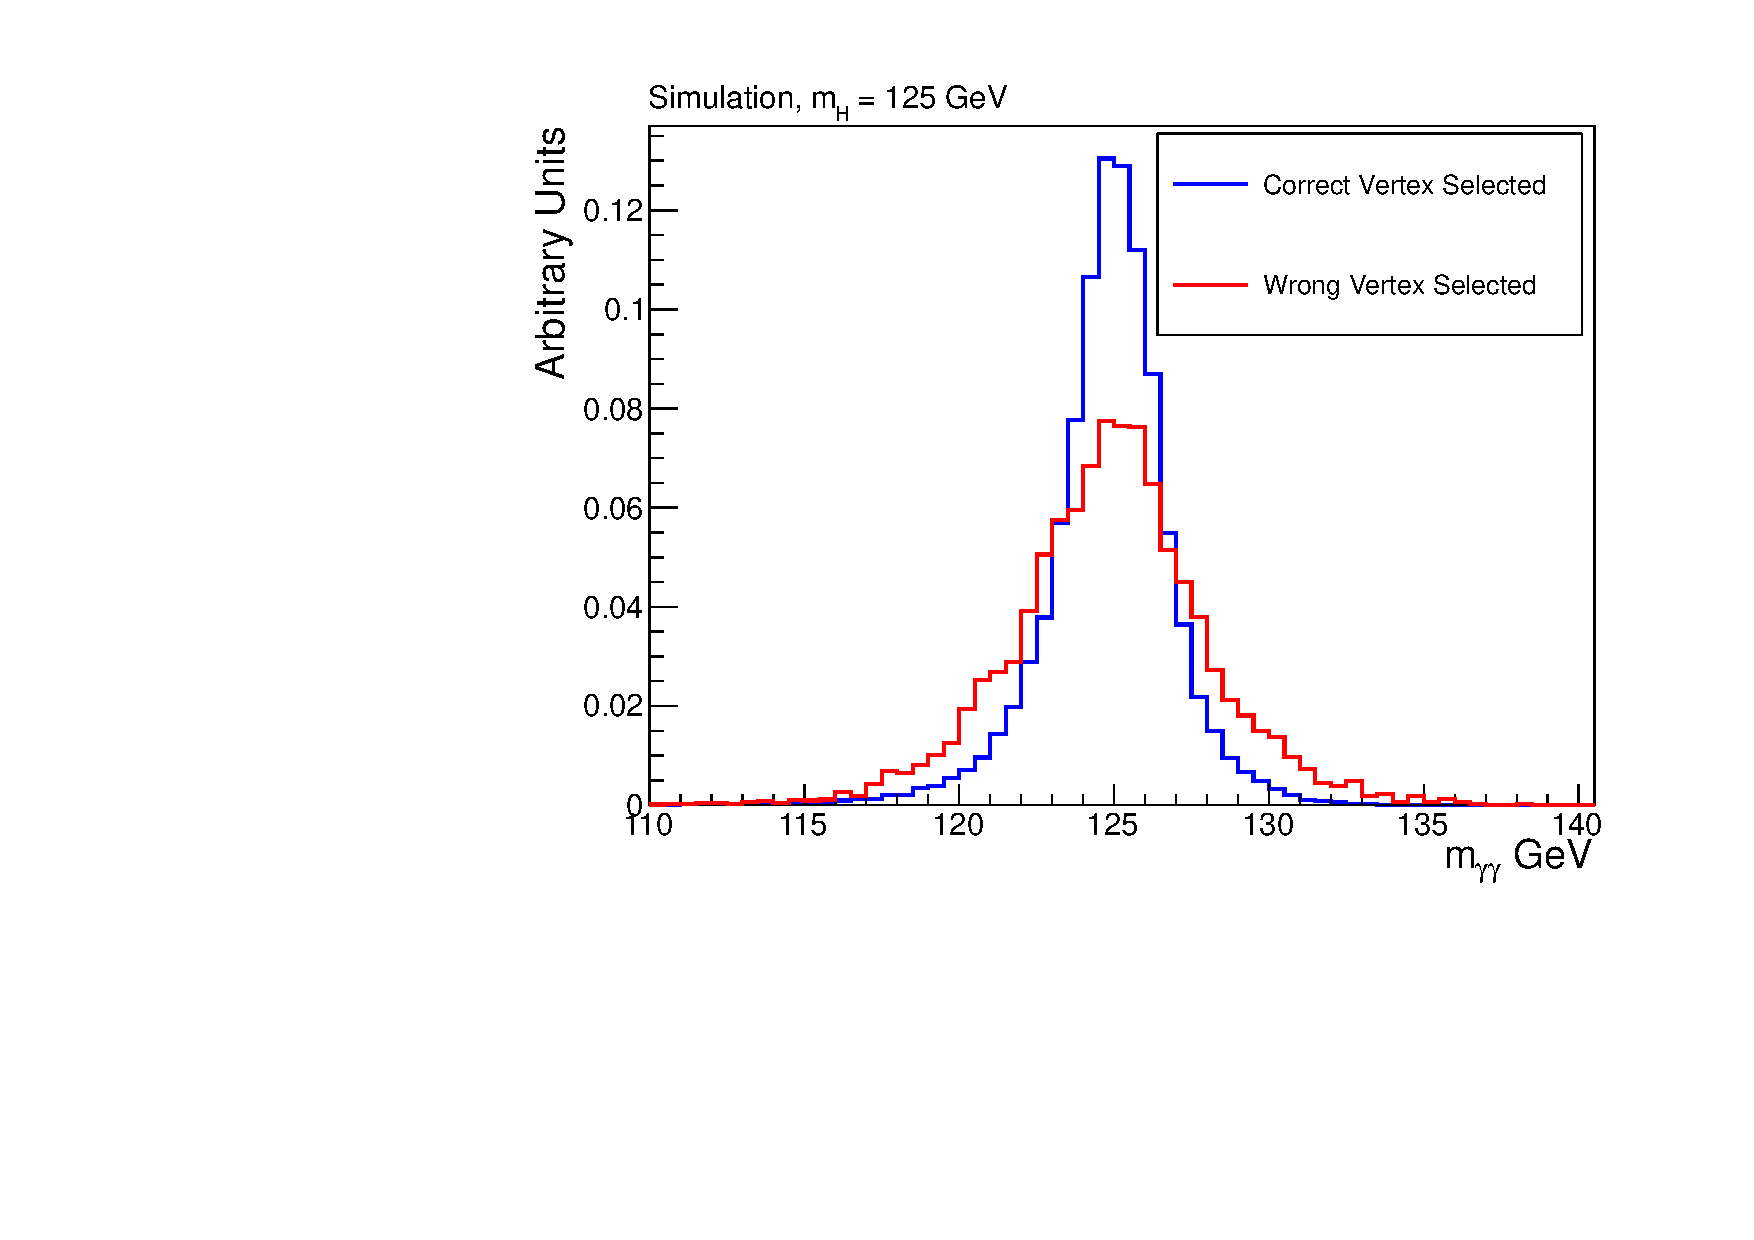
\includegraphics[width=.8\textwidth]{hgg7TeV/generalPlots/rightwrongvtxpeak.pdf}
\label{fig:higgsrightwrongvertex}
\caption{Invariant mass peak in $\Hgg$ MC with mass 125 GeV. The blue histogram is from events in which 
the generated vertex is within 10mm of the vertex assigned to the diphoton pair. The red histogram is 
from events in which the incorrect vertex is assigned. Both distributions are normalised to unit area for
ease of comparison.}
\end{center}
\end{figure} 

A BDT was trained to rank the standard collection of reconstructed vertices.
The input variables are chosen to exploit the correlation between the diphoton system and the recoiling tracks.
These are the $\pt$-balance and $\pt$-asymmetry calculated as,

\begin{eqnarray}
	-\sum_{all tracks} \left(\ptvec^{track}\cdot \frac{\displaystyle \ptggvec}{\displaystyle \ptgg}\right) 
\end{eqnarray}
and
\begin{eqnarray}
	\frac{\displaystyle |\sum_{all tracks} \ptvec^{track}| - \ptgg }{ \displaystyle|\sum_{all tracks} \ptvec^{track}|} 
\end{eqnarray}

respectively. In addition, the sum of the square of the transverse momenta of all the tracks associated 
to a given vertex is included to preferentially select hard interactions. If at least one of the 
photons converts to an $e^{+}e^{-}$ pair, the difference between the position in $z$ as calculated 
using the electron-positron pair and that from the standard vertex, relative to the resolution in $z$
is included as an input variable. The BDT was trained on $\Hgg$ MC with a mass of 120 GeV. 
Figure~\ref{fig:vtxeffhmc} shows the fraction of events in a gluon-gluon MC sample in which 
the vertex with the highest BDT score is within 10mm of the true vertex as a function of $\pt^{H}$.

\begin{figure}
\begin{center}
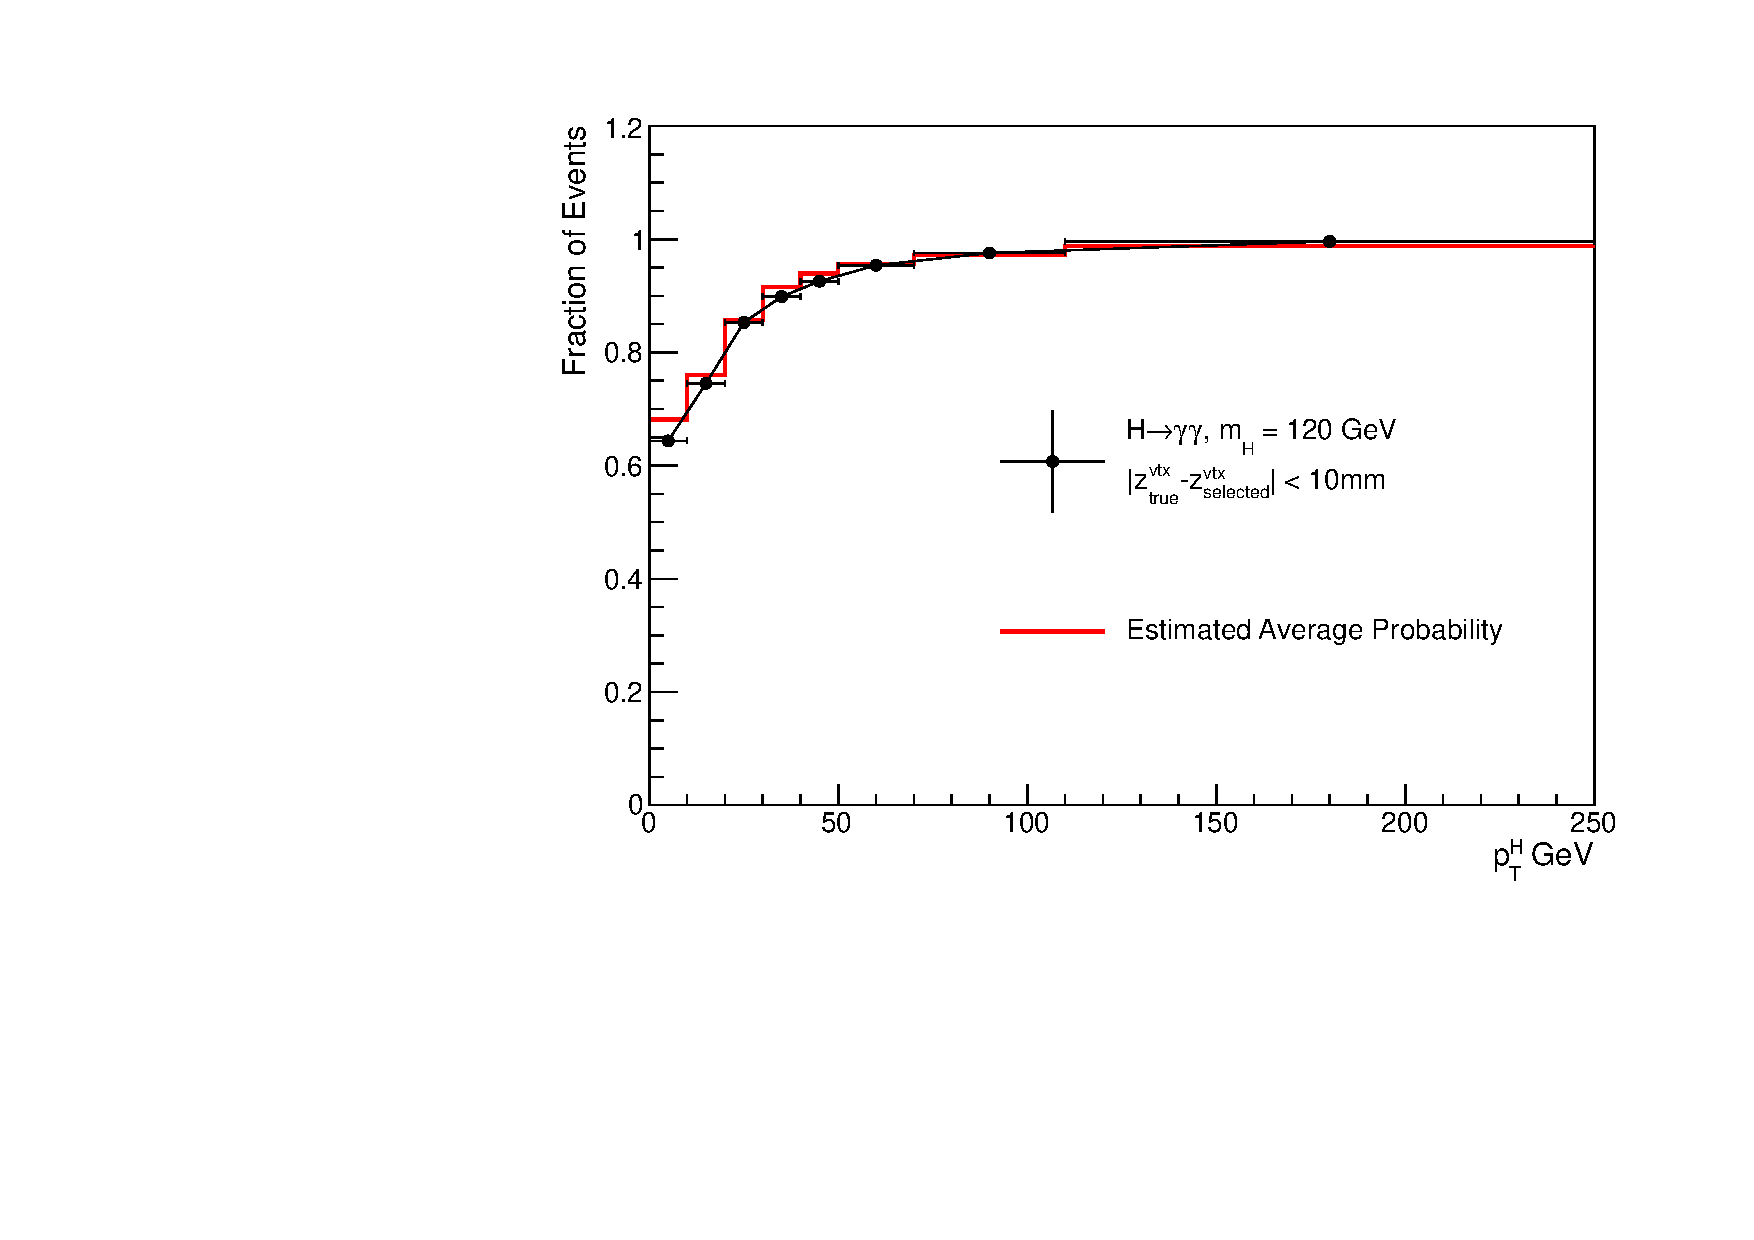
\includegraphics[width=.8\textwidth]{hgg7TeV/generalPlots/vtxEffHMC.pdf}
\caption{Fraction of simulated gluon-gluon fusion events in which the selected vertex $z$ position 
is within 10mm of the true vertex as a function of Higgs $\pt$. The red histogram is the average 
probability to select the correct vertex in each bin estimated from the per-event BDT.}
\end{center}
\label{fig:vtxeffhmc}
\end{figure} 

The fraction of events in which this occurs in data is measured using $\Zmumu$ events
as a function of the $\pt$ of the $Z$ boson~\ref{AN-11-048}. This is used to correct the Higgs signal MC for 
the purpose of signal modelling. A second, per-event BDT is trained using the output of the first, to identify 
under which conditions the correct vertex is selected. The output of this BDT is then used to 
calculate the probability in a given event that the correct vertex is assigned. The red line in Figure~\ref{fig:vtxeffhmc}
shows a comparison of the per-event vertex probability estimated from the second BDT against the 
fraction of the events in which the selected vertex is located within 10mm from the true vertex.

\subsection{Photon Identification}
\label{sec:photonidentification}

A large portion of the fake background in the $\Hgg$ search is due to high momentum neutral mesons
which decay to two photons where both the photons are combined into the same supercluster~\cite{HIG-11-033}. 
Information from the shower shape of the photon supercluster can be used, in addition to the 
energy isolation within the calorimeter, in order to distinguish these from prompt photons
from the primary interaction point. A BDT was trained on MC events to combine the relevant information
into a single photon identification (ID) discriminator. The signal used for the training was taken from 
simulated $\Hgg$ events with a Higgs boson mass of 121 GeV while the background was 
taken from non-prompt photons in the Gamma+Jet sample.
Before training, events are required to pass a loose preselection designed to avoid training 
where the MC is unable to properly describe the data and to match the variables used in the trigger~\cite{AN-12-048}.
In addition, photon candidates are removed if there is a reconstructed \texttt{GsfElectron} matched to the 
photon supercluster with no matching conversion reconstruction. This greatly reduces the contribution
from $\Zee$ faking photons. The same preselection is applied to all MC and data for extracting the signal.
The efficiency of the preselection for signal was measured in $\Zee$ data and MC using a tag-and-probe 
method~\cite{AN-12-116}. The results are shown in Table~\ref{tab:sigeffpresel}. 

\begin{table}
\begin{center}
\begin{tabular}{| l | c | c | c |}
\hline
\textbf{Category} & \textbf{Data} & \textbf{MC} & \textbf{Data/MC} \\
\hline
EB $\rnine>0.9$ & 0.9267 $\pm$ 0.0012 & 0.9275 $\pm$ 0.0006 &0.999 $\pm$ 0.0013 \\
EB $\rnine<0.9$ & 0.8882 $\pm$ 0.0023 & 0.9025 $\pm$ 0.0010 &0.984 $\pm$ 0.0025 \\
EE $\rnine>0.9$ & 0.9442 $\pm$ 0.0010 & 0.9387 $\pm$ 0.0009 &1.006 $\pm$ 0.0014 \\
EE $\rnine<0.9$ & 0.8639 $\pm$ 0.0010 & 0.8517 $\pm$ 0.0011 &1.014 $\pm$ 0.0015 \\
\hline
\end{tabular}
\caption{Signal efficiency for the preselection measured in data and MC using tag-and-probe in
$\Zee$ events. The ratio Data/MC are applied as corrections to the signal MC for the purposes
of signal modelling. The uncertainties listed here are statistical only.}
\label{tab:sigeffpresel}
\end{center}
\end{table}

The input variables are chosen to be insensitive to the kinematics of the diphoton system itself
including the diphoton invariant mass. The first set of variables describe the shower shape of the 
supercluster: $\hoe$, $\sigieie$, $\rnine$ and the energy weighted widths of the supercluster in
$\eta$ and $\phi$ ($\sigma_{\eta},~\sigma_{\phi}$). The $\eta$ of the supercluster is 
included as the shower shape is dependant on the position within the calorimeter. 
The second set of input variables describe the
isolation of the photon in the calorimeter and tracker scaled to account for 
the additional expected energy density due to pileup, $\rho$~\cite{2011JInst611002C}. 
These are the sum of the track isolation, 
calculated relative to the chosen vertex and the vertex giving the maximum track isolation,
ECAL isolation and HCAL isolation in a cone with $\Delta R<0.3$ minus $\rho$ times the effective area 
of the cone~\cite{2011JInst611002C}.
and the absolute ECAL and HCAL isolations within cones of $\Delta R <0.3$ and $\Delta R<0.4$ 
respectively. In addition, the number of reconstructed vertices in the bunch crossing is included
to reduce the pileup dependence of the isolation variables. 

A separate BDT is trained for application in the ECAL barrel and endcaps as the shower
shape and isolation variables are rather distinct between the two components. 
A cut is made on the photon ID BDT output to select events used for the signal extraction which
keeps practically all ($>99\%$) of the signal while removing around 22\% of background events.
The cut is chosen to be loose as the output of the photon ID will be used as input for the 
event selection (diphoton BDT) as described in Section~\ref{sec:diphotonbdt}. 

\section{Event Selection}
\label{sec:eventselection}

In addition to passing the preselection, the two photons are required to pass mass-dependant transverse 
momenta cuts, $p_{T}/\mgg > 1/3, ~1/4$ for the leading and subleading photon respectively.
Where more than one diphoton pair satisfies these criteria in an event, the pair which has the largest
sum of photon transverse momenta is selected as the Higgs candidate.
The final selection of diphoton candidates used for the signal extraction is based on using as much information 
in the event as possible to distinguish likely signal candidate events from the background. Although the 
photon ID BDT is successful at rejecting fake backgrounds, a large portion of the background is due to
real prompt diphotons from QCD processes. In order to distinguish these from a Higgs signal, 
the specific kinematics and topology of the event are exploited.

\subsection{Diphoton BDT}
\label{sec:diphotonbdt}
A BDT was trained to utilise the kinematics of the selected diphoton pair to discrimiate prompt photons
from QCD background from those produced by the decay $\Hgg$. The BDT was trained using the QCD Dijet,
Gamma+Jet, DiphotonJets and Diphoton Born samples for background and Higgs MC with a mass of 123 GeV.
As the mass of the Higgs boson is unkown, the search is performed under different mass hypotheses.
In order to allow for the application of the same selection to the data under any mass hypothesis,
the input variables to the BDT are chosen to be mass-independant. In addition, this allows
for a fully data-driven estimation of the background shape as described in Section~\ref{sec:backgroundmodel}.
The input variables which describe the kinematics are:
the relative transverse momenta of the photons, $\pt^{1},~\pt^{2}$, 
their pseudo-rapidites, $\eta^{1},~\eta^{2}$ and the cosine of the 
angle between the two photons in the transverse plane $cos(\Delta\phi)=cos(\phi^{1}-\phi^{2})$.
In addition, information regarding the quality
of the objects, the two photons and the selected vertex, is included in the form of the output of the 
photon ID and the vertex probability. The per-photon resolution estimate, $\sigma_{E}$ is combined for
each photon to produce a per-event mass resolution estimate ($\sigma_{\mgg}$) under the assumption that 
the correct vertex is selected;

\begin{equation}
\sigma_{\mgg} (right-vtx) = \frac{\displaystyle \mgg}{\displaystyle 2} 
\sqrt{ \left( \frac{\displaystyle {\sigma_{E}^{1}}}{\displaystyle E^{1} } \right)^{2}
     + \left( \frac{\displaystyle {\sigma_{E}^{2}}}{\displaystyle E^{2} } \right)^{2}
     }
\end{equation}
where $E^{1},~E^{2}$ are the energies of the two photons.

Since the correct vertex is not always selected, the mass resolution assuming the incorrect vertex is chosen
is calculated using the average beamspot length in data, $\sigma_{Z}=5.8$cm. In this case, the distance 
between the selected and true vertex will be distributed as a Gaussian with width $\sqrt{2}\sigma_{Z}$.
The contribution to the resolution, $\sigma_{\mgg}^{vtx}$, can be calculated analystically given the positions of
the two photons. The mass resolution estimator under the assumption that the incorrect vertex is chosen is 
given by the sum in quadrature of $\sigma_{\mgg}^{vtx}$ with the mass resolution assuming the correct vertex is chosen.
Both estimators for the mass resolution relative to the invariant mass, $\sigma_{\mgg}/\mgg~$ right/wrong-vtx, 
are included as inputs to the diphoton BDT. Figure~\ref{fig:diphotonBDT} shows the diphoton BDT distribution in 
data and MC. In addition to further separating the contribution to the background from fakes, the diphoton BDT 
can discriminate between prompt diphotons in QCD and those from a $\Hgg$ decay. The final events used for 
the signal extraction are selected as those with a diphoton BDT output greater than 0.05. This cut is chosen
following an optimization study to minimize the expected exclusion limit in the absence of signal.
Events below this cut value were found to provide negligible improvement in the expected limit~\cite{AN-12-048}.

\begin{figure}[hbt!]
\begin{center}
 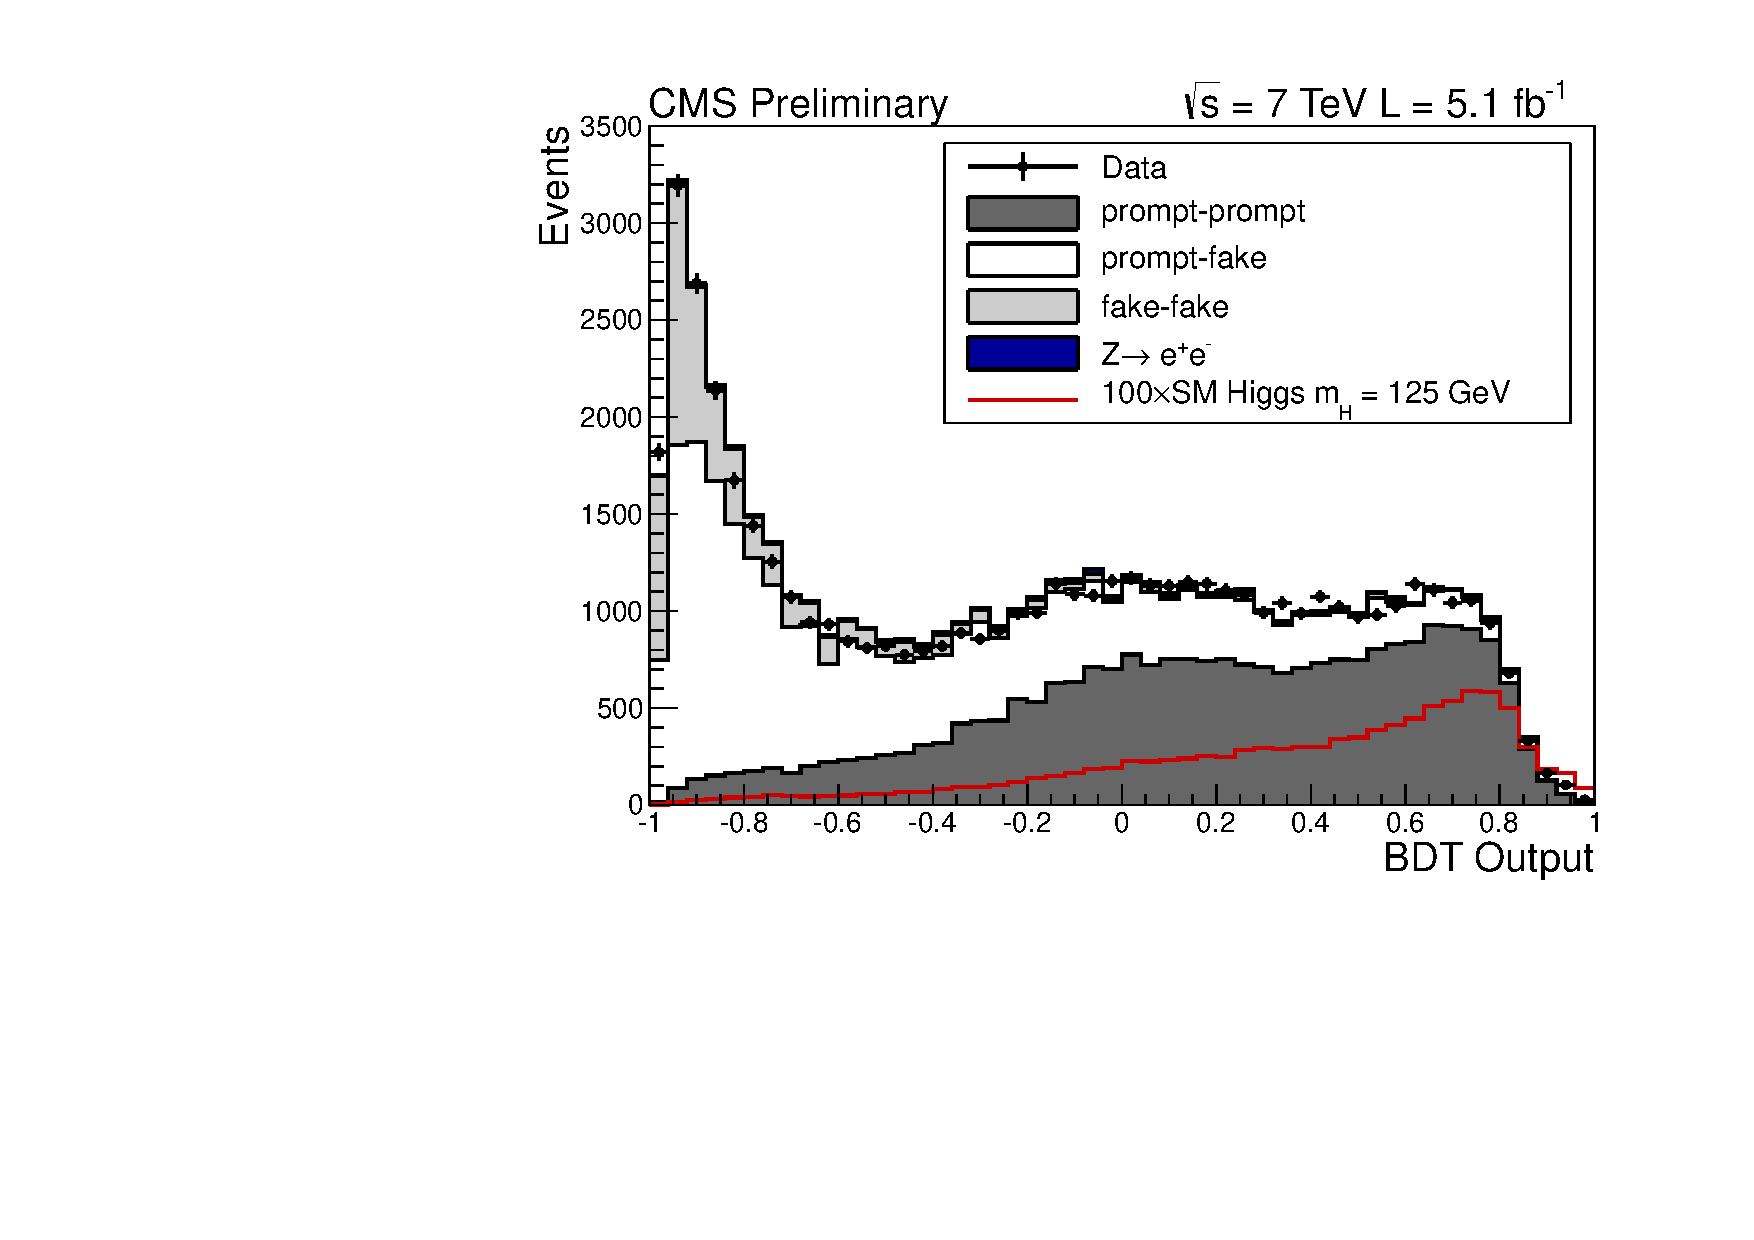
\includegraphics[width=0.8\textwidth]{hgg7TeV/variablePlots/bdtoutput_full}
 \caption{Diphoton BDT distribution in data and MC. The contribution expected from a SM Higgs with mass 125 GeV, 
 scaled by 100, is shown in red. }
 \label{fig:diphotonBDT}
\end{center}
\end{figure}

Figures~\ref{fig:diphotonbdtvars1} and~\ref{fig:diphotonbdtvars2} show the input variables from the 
final set of selected diphoton candidates in data and MC. 
The expectation in each plot from a SM Higgs with a mass of 125 GeV, scaled by 10, is shown in red. 
The invariant mass distribution in data and MC for events passing the full
selection is given in Figure~\ref{fig:massmcdata}. After the application of the full selection, 
the total background contains around 76\% prompt diphoton events.

\begin{figure}[hbt!]
\begin{center}
  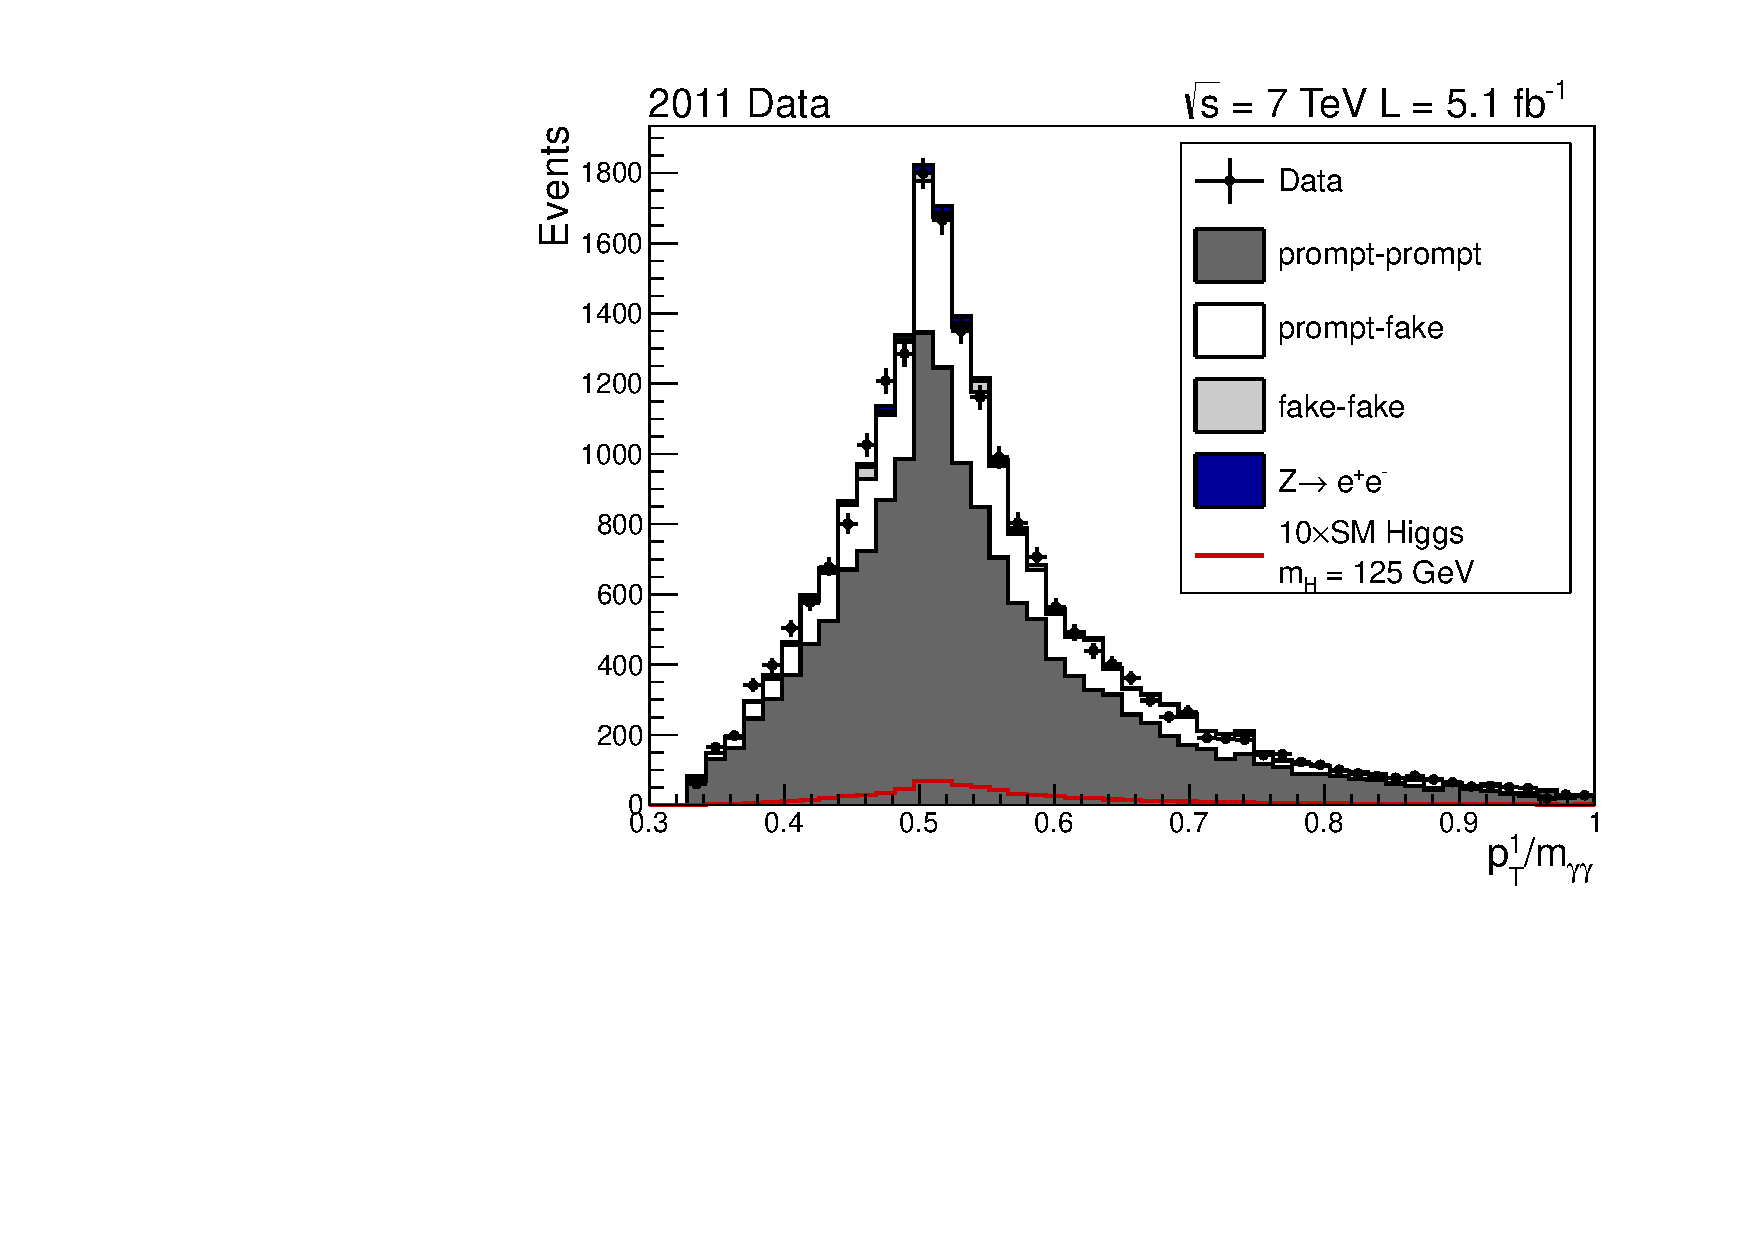
\includegraphics[width=0.48\textwidth]{hgg7TeV/variablePlots/pt_1om}
  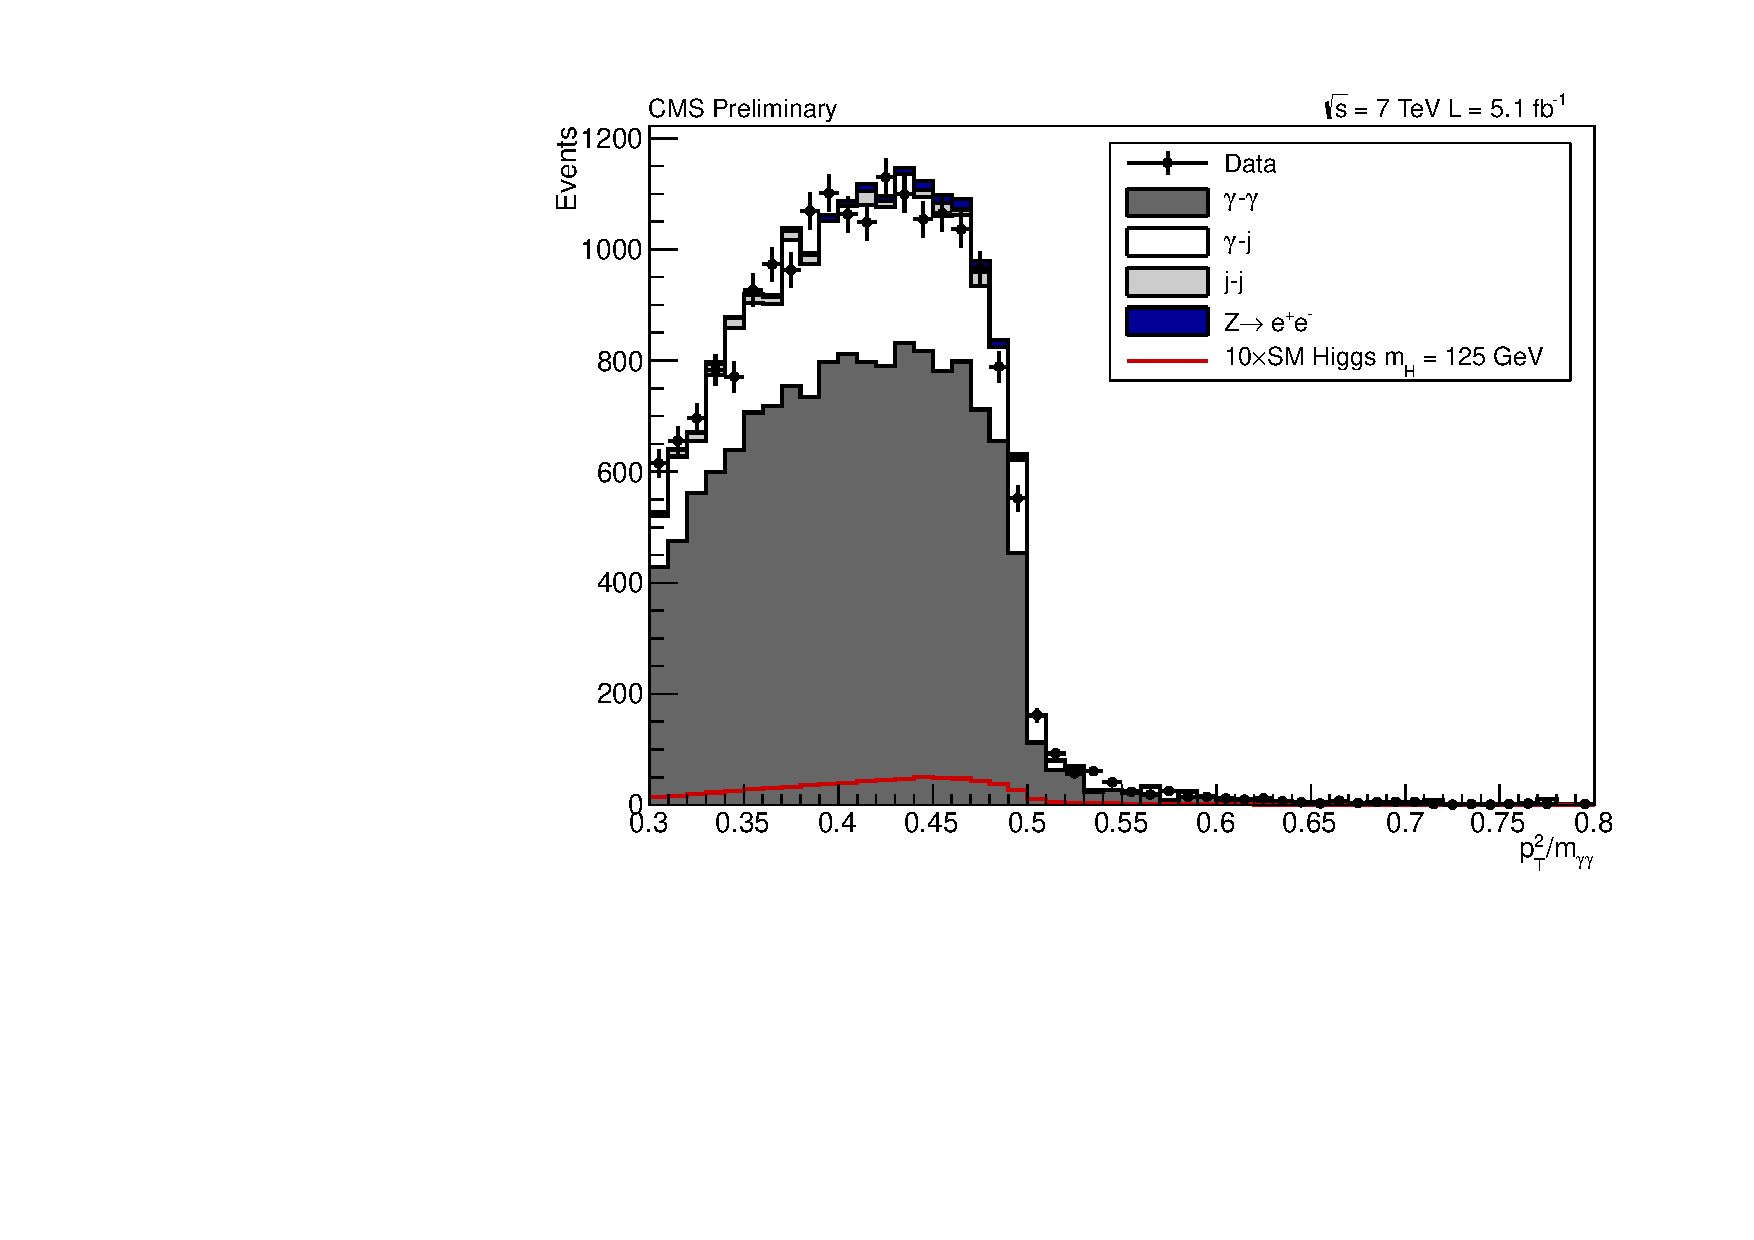
\includegraphics[width=0.48\textwidth]{hgg7TeV/variablePlots/pt_2om}\\
  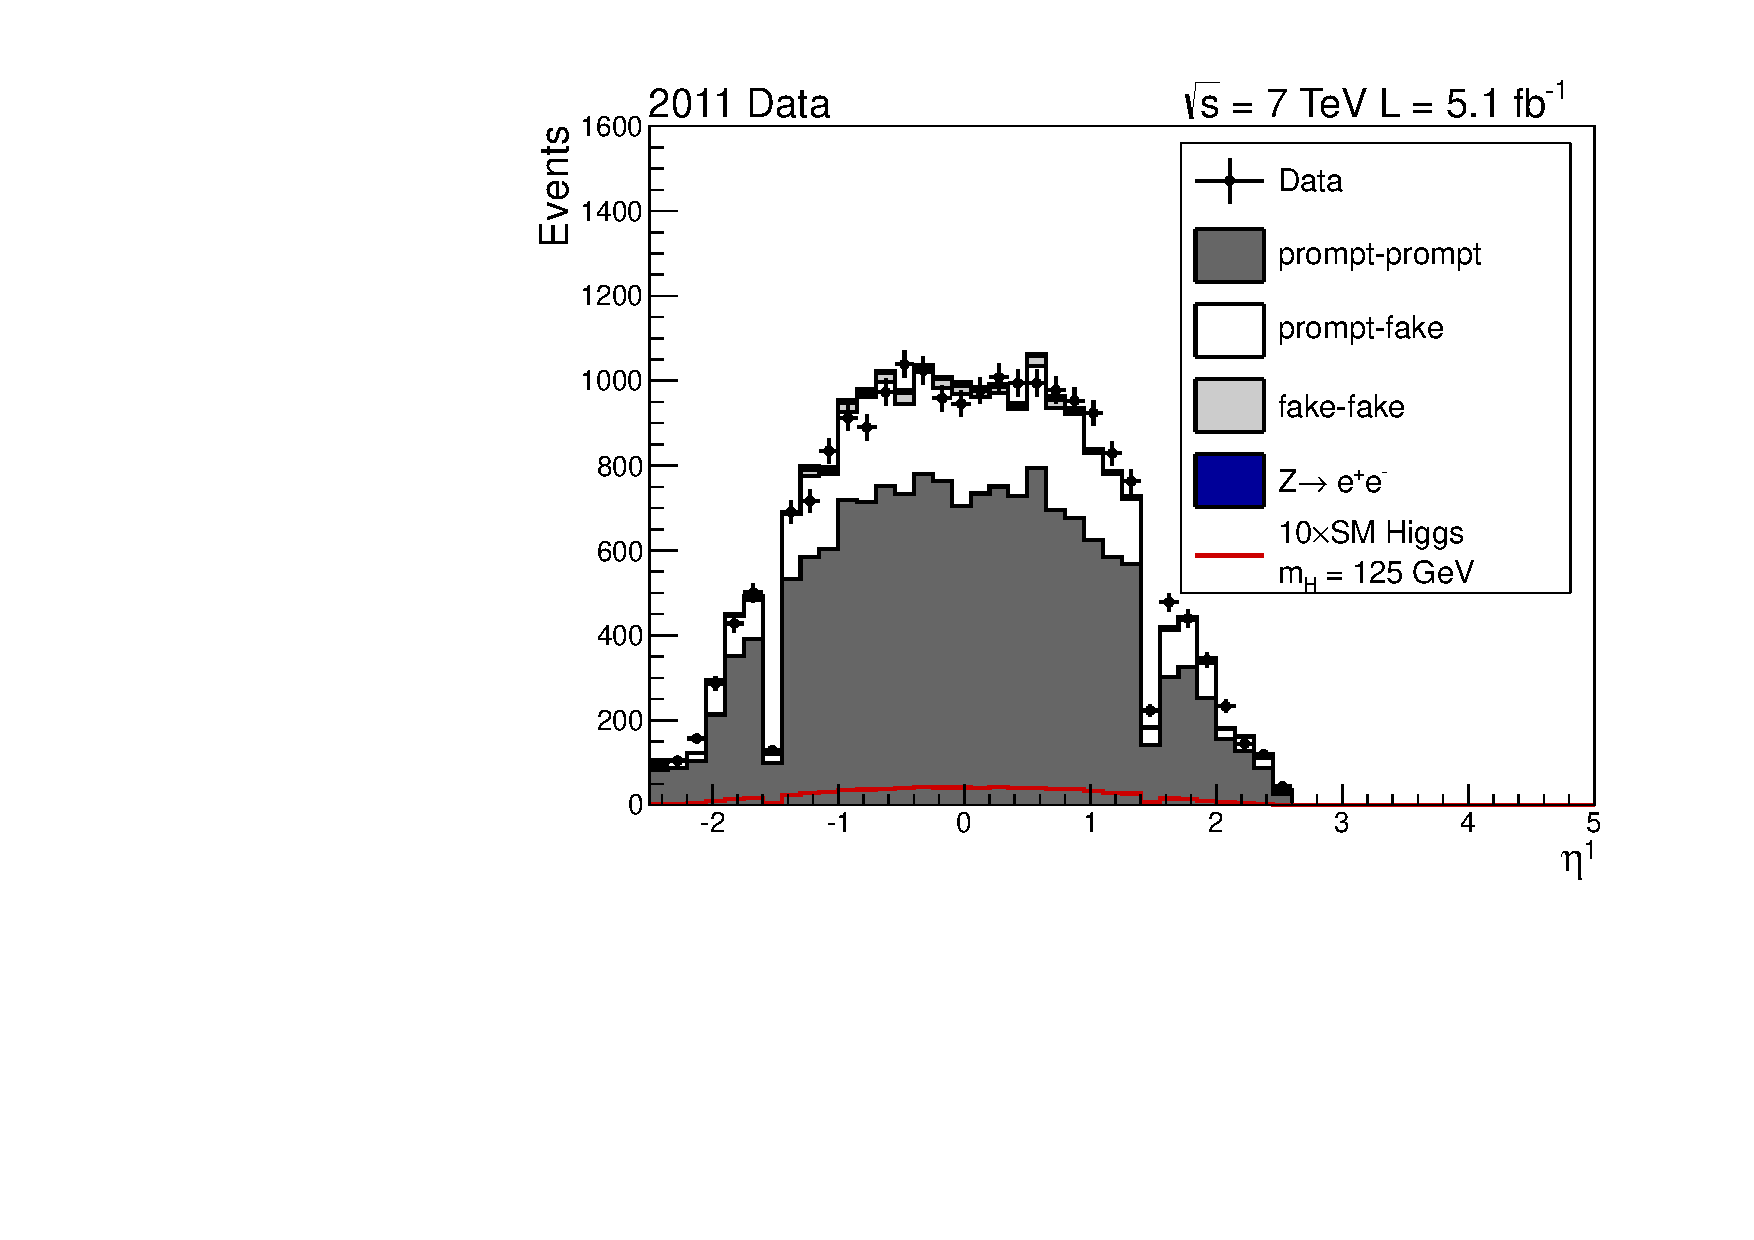
\includegraphics[width=0.48\textwidth]{hgg7TeV/variablePlots/phoeta_1}
  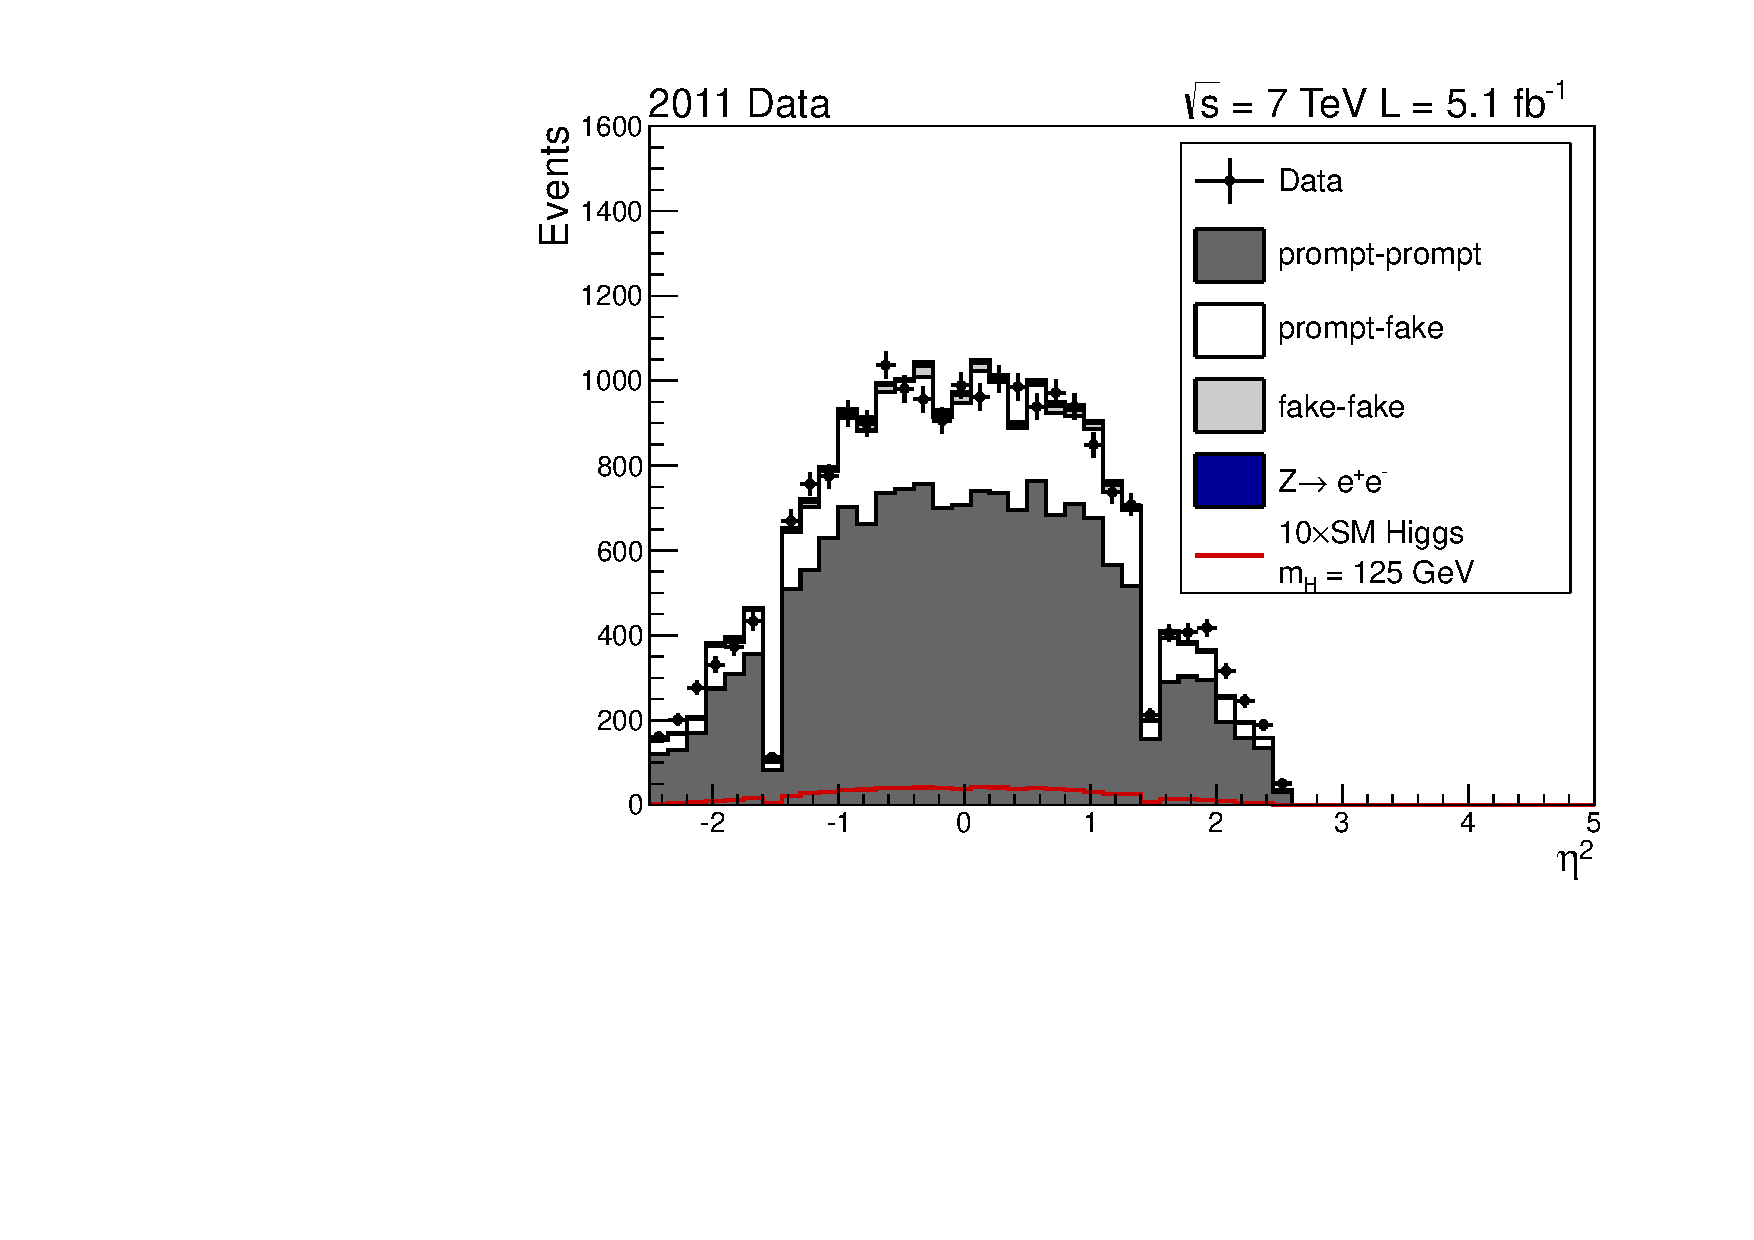
\includegraphics[width=0.48\textwidth]{hgg7TeV/variablePlots/phoeta_2}\\
  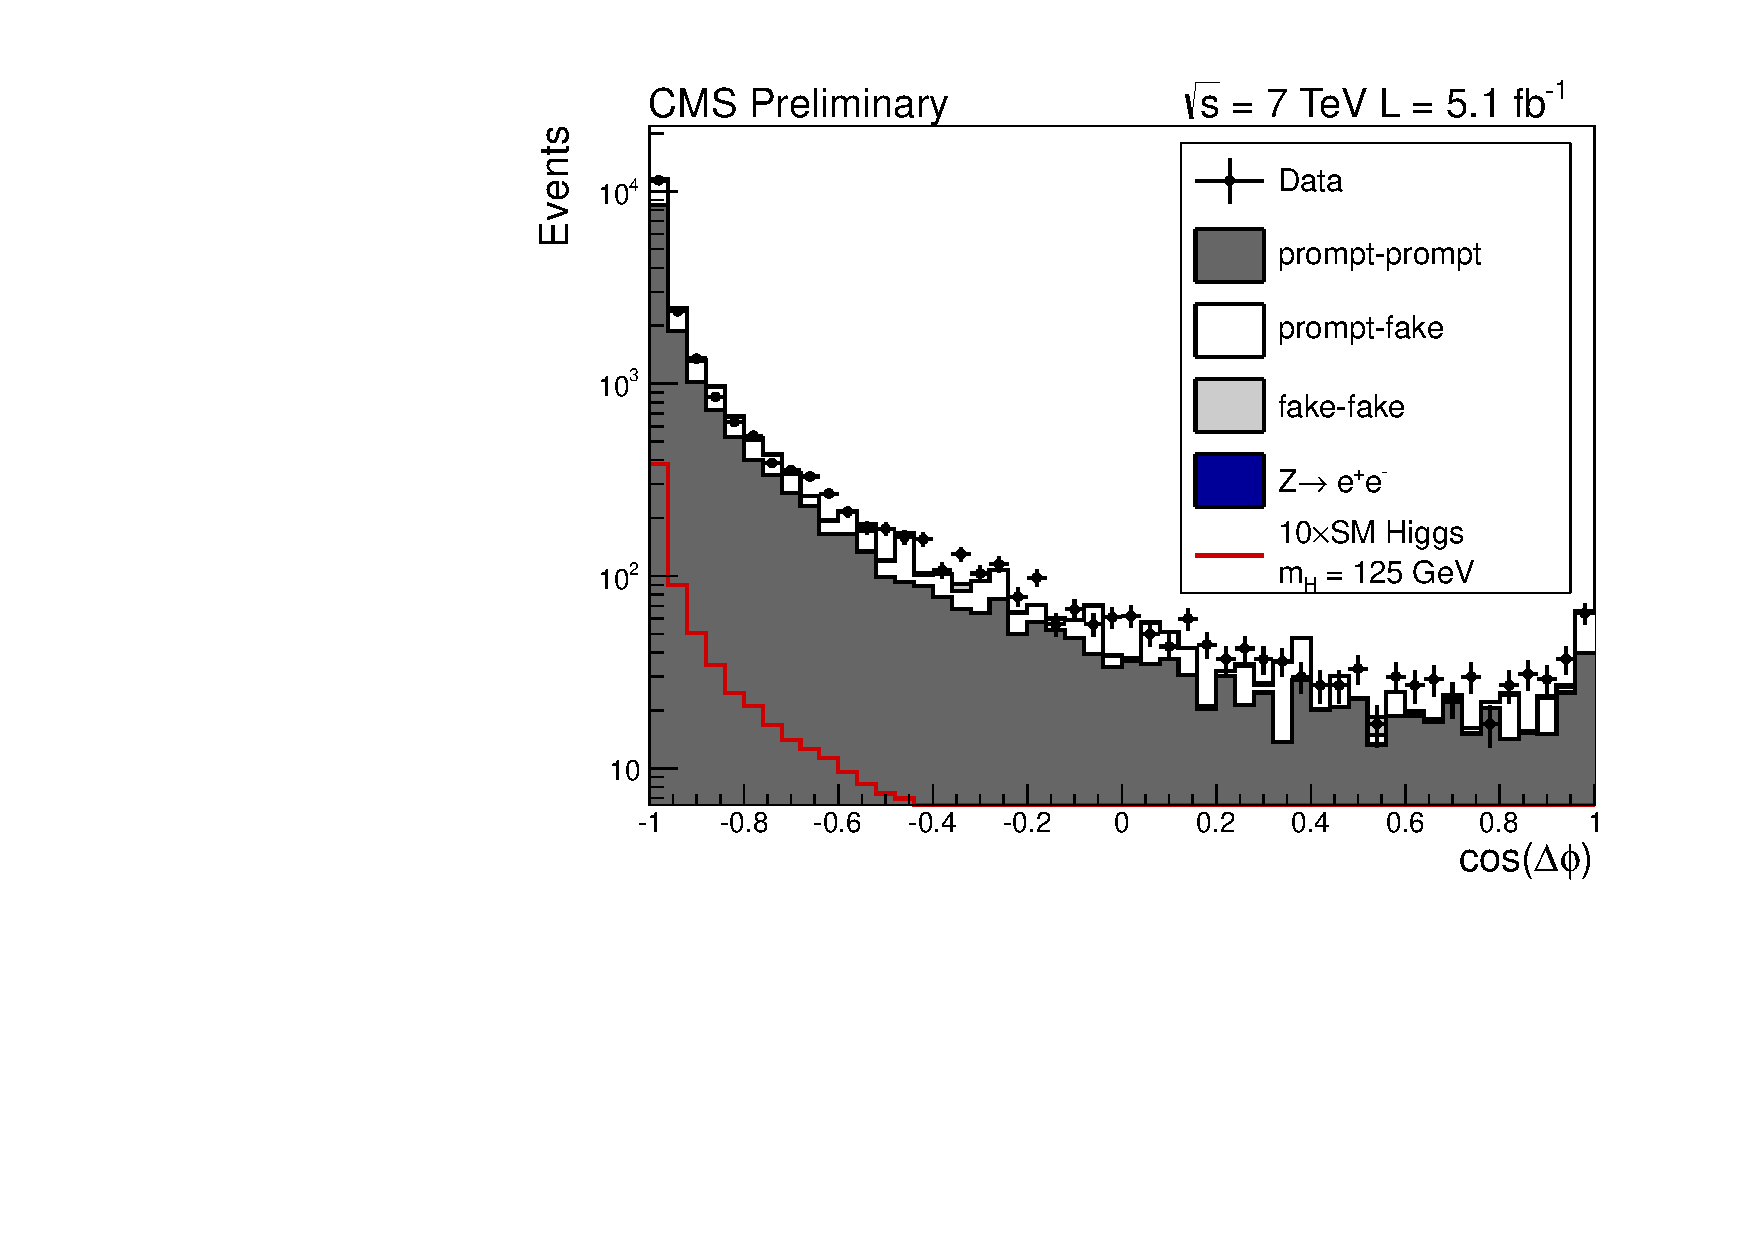
\includegraphics[width=0.48\textwidth]{hgg7TeV/variablePlots/cosdphi}
 \label{fig:diphotonbdtvars1}
 \caption{Kinematic diphoton BDT input variable distributions in data and MC. 
	  The distributions are for events which pass the full selection 
	  including a cut on the diphoton BDT output of 0.05.
 	  The expectation from a SM Higgs with 125 GeV is shown in red.}
\end{center}
\end{figure}

\begin{figure}[hbt!]
\begin{center}
  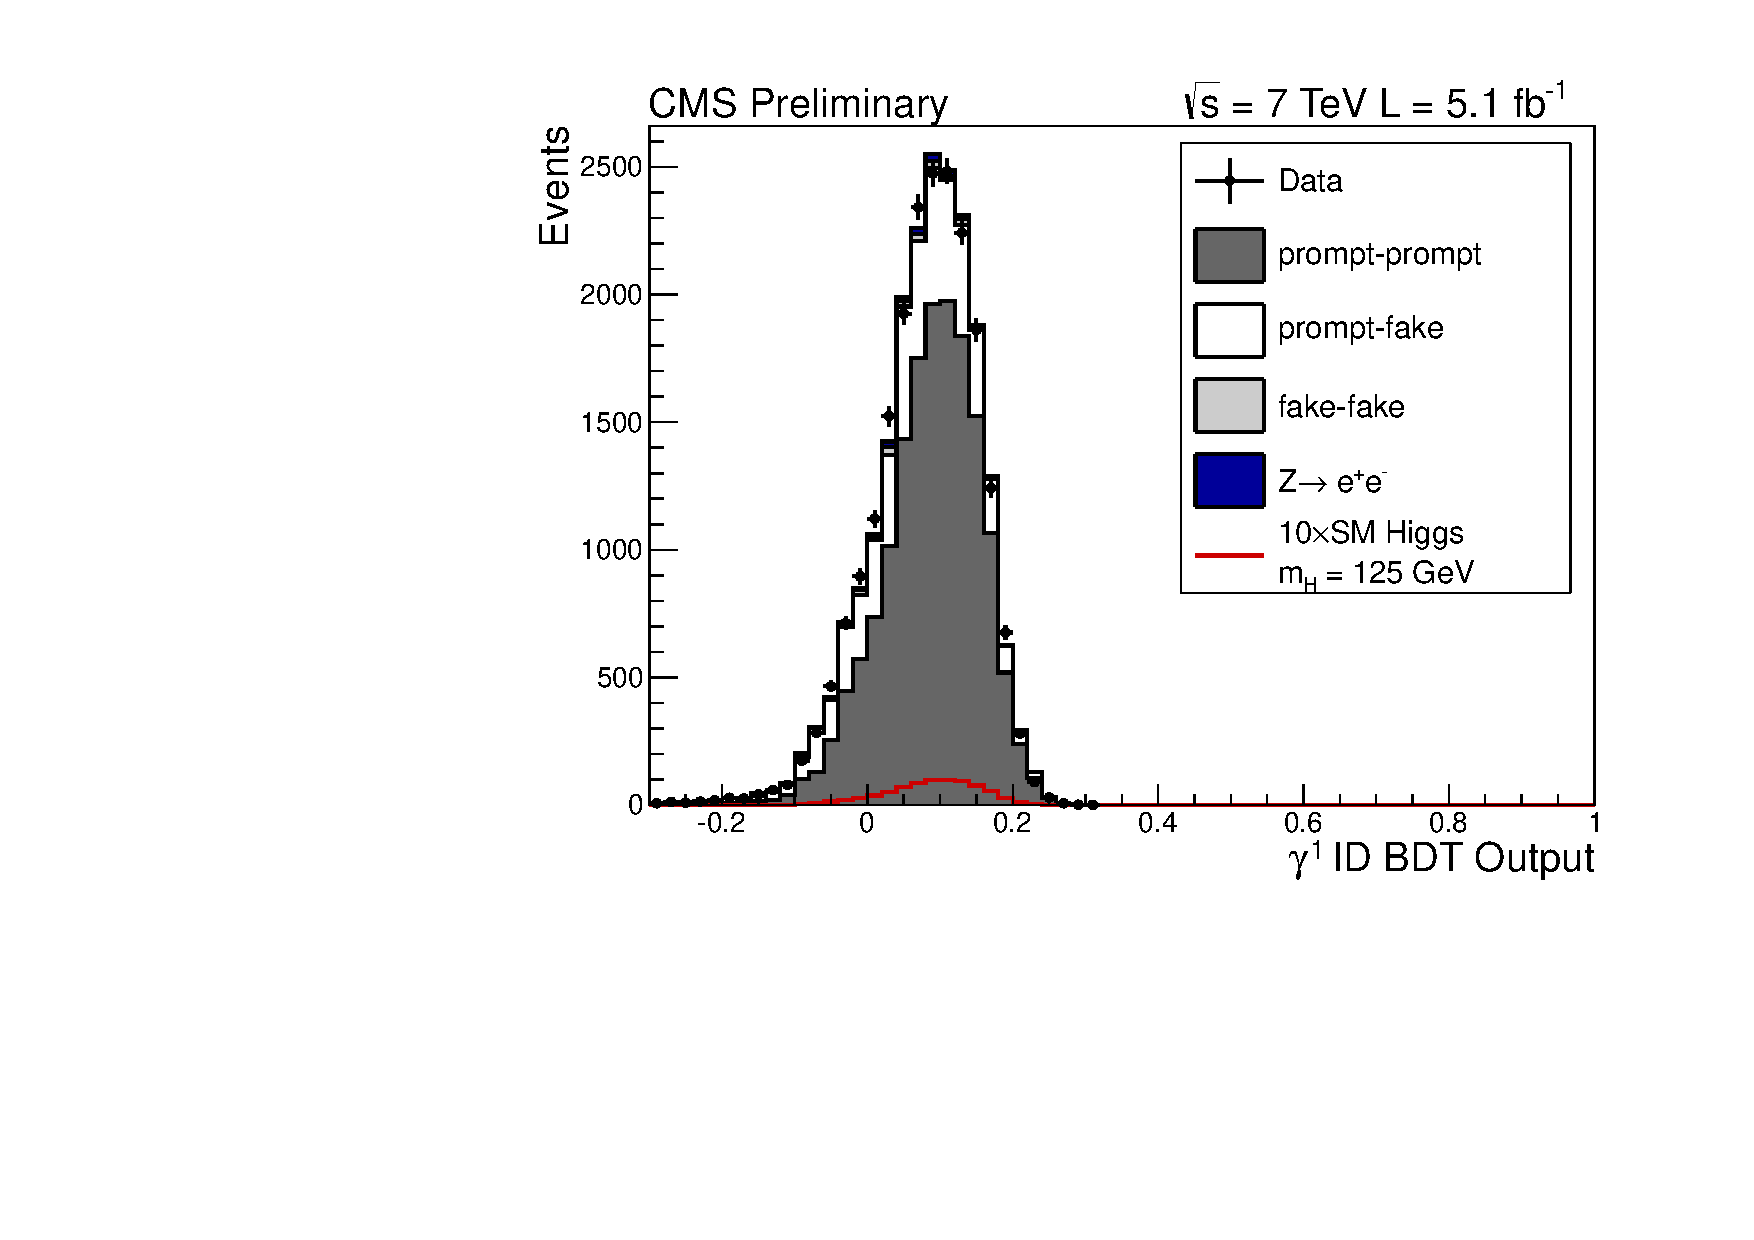
\includegraphics[width=0.48\textwidth]{hgg7TeV/variablePlots/phoid_1}
  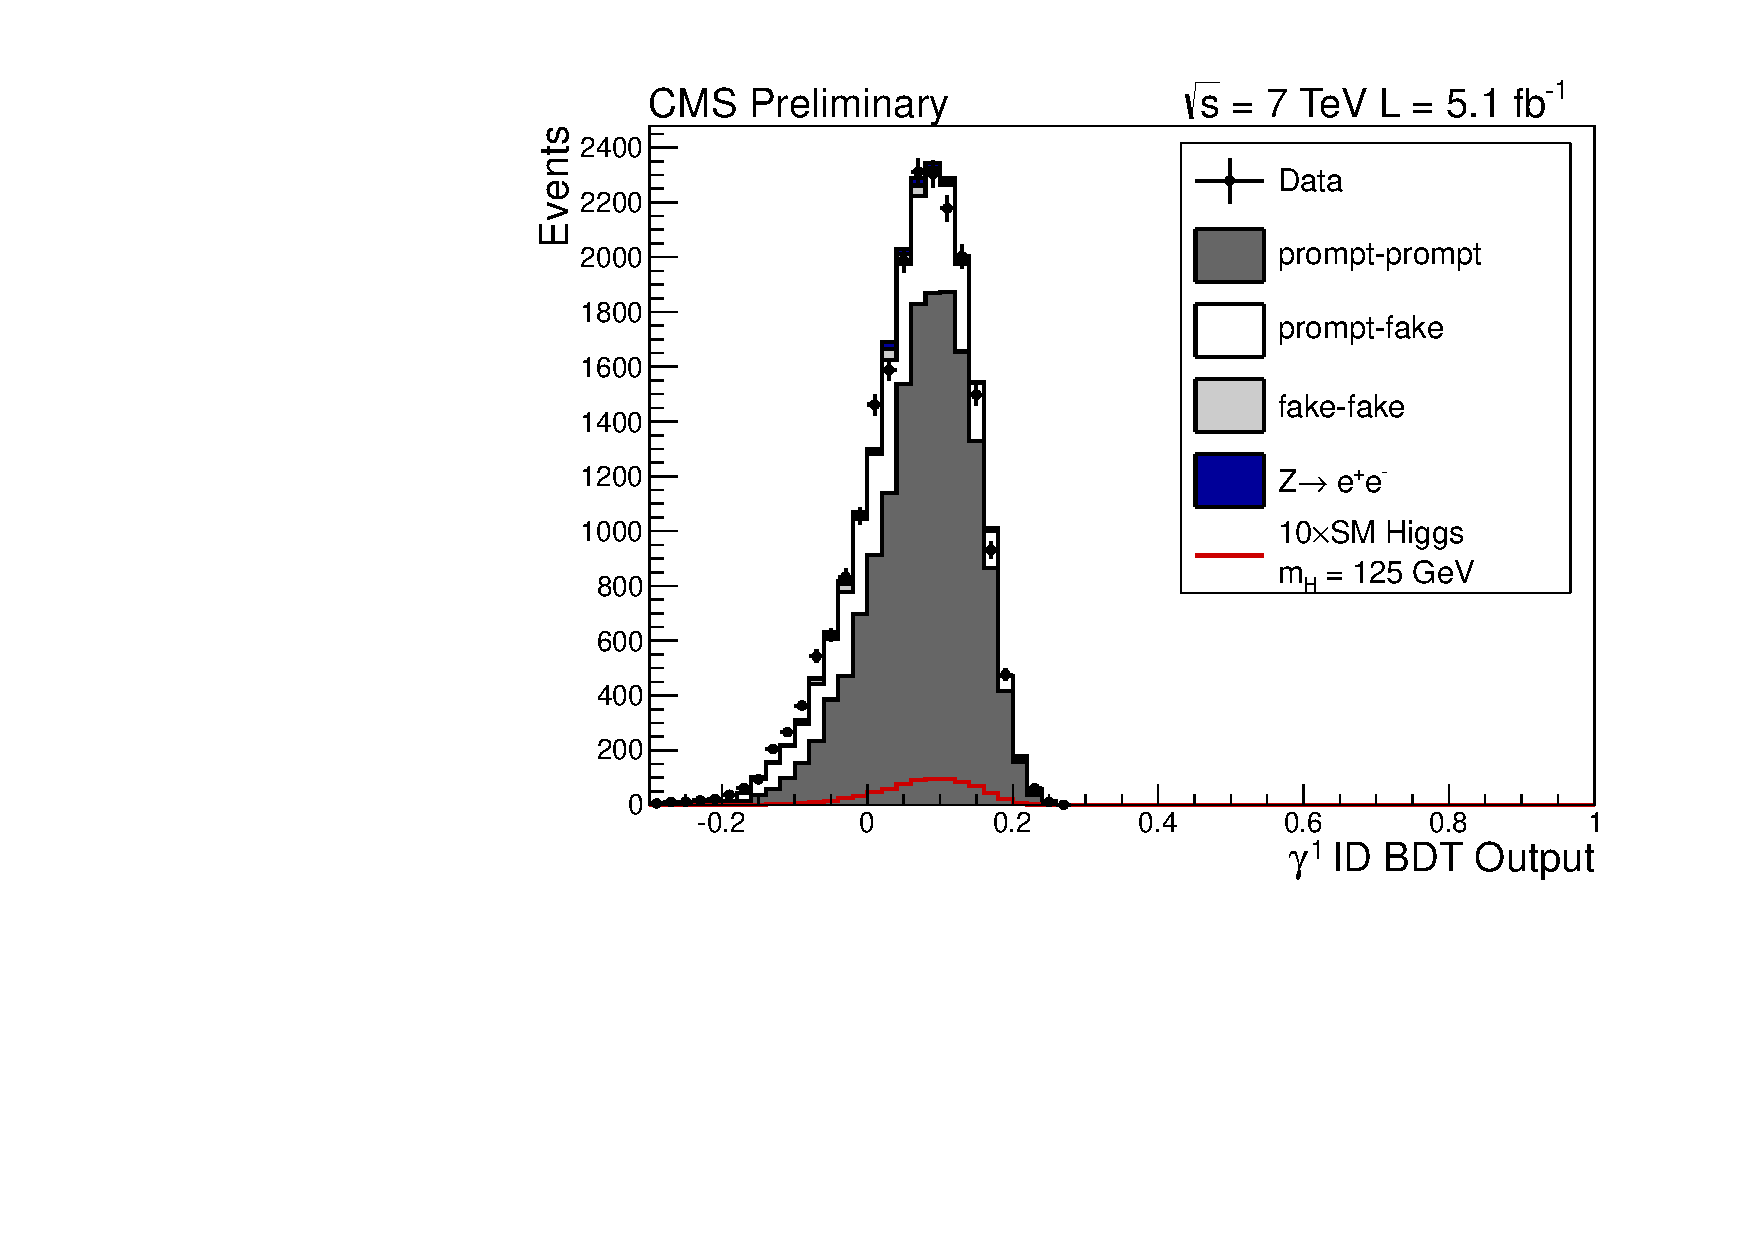
\includegraphics[width=0.48\textwidth]{hgg7TeV/variablePlots/phoid_2}\\
  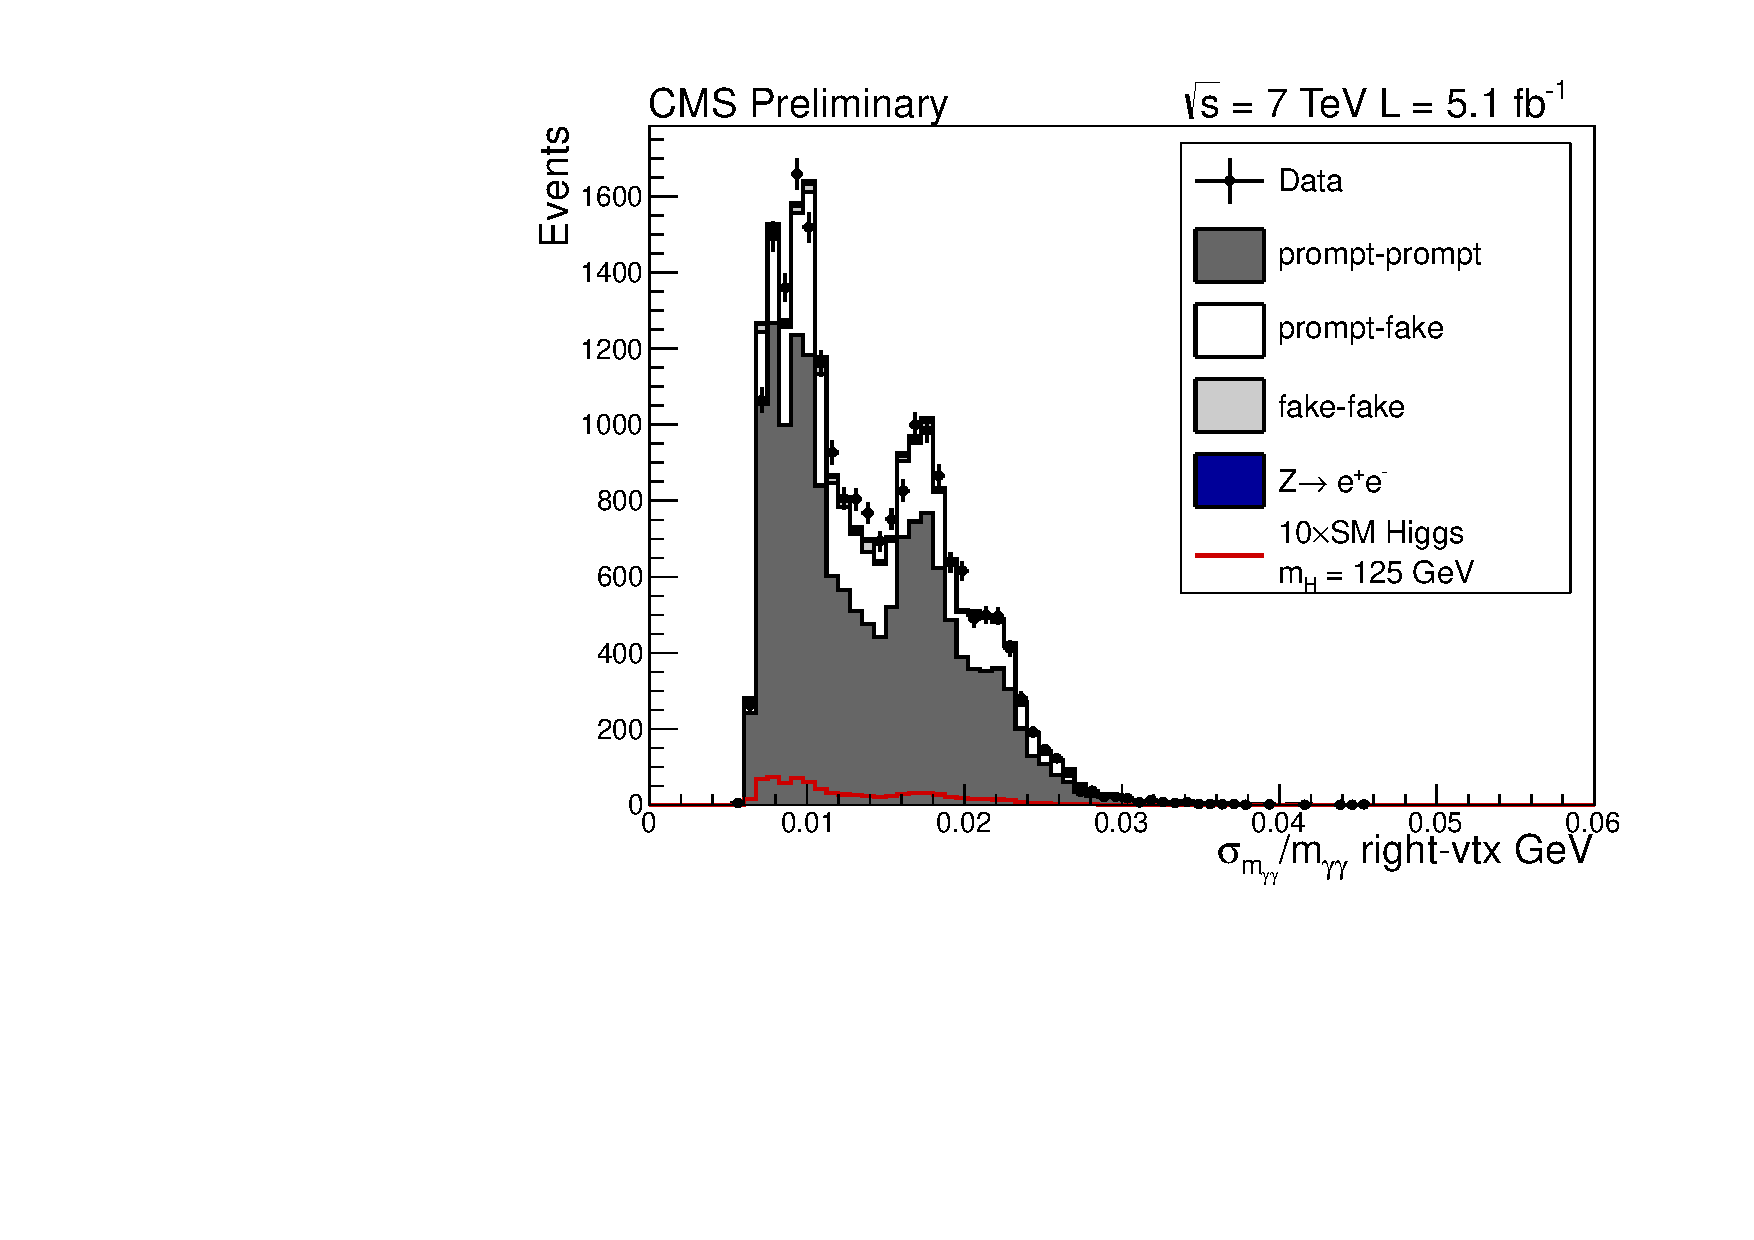
\includegraphics[width=0.48\textwidth]{hgg7TeV/variablePlots/sigmrv}
  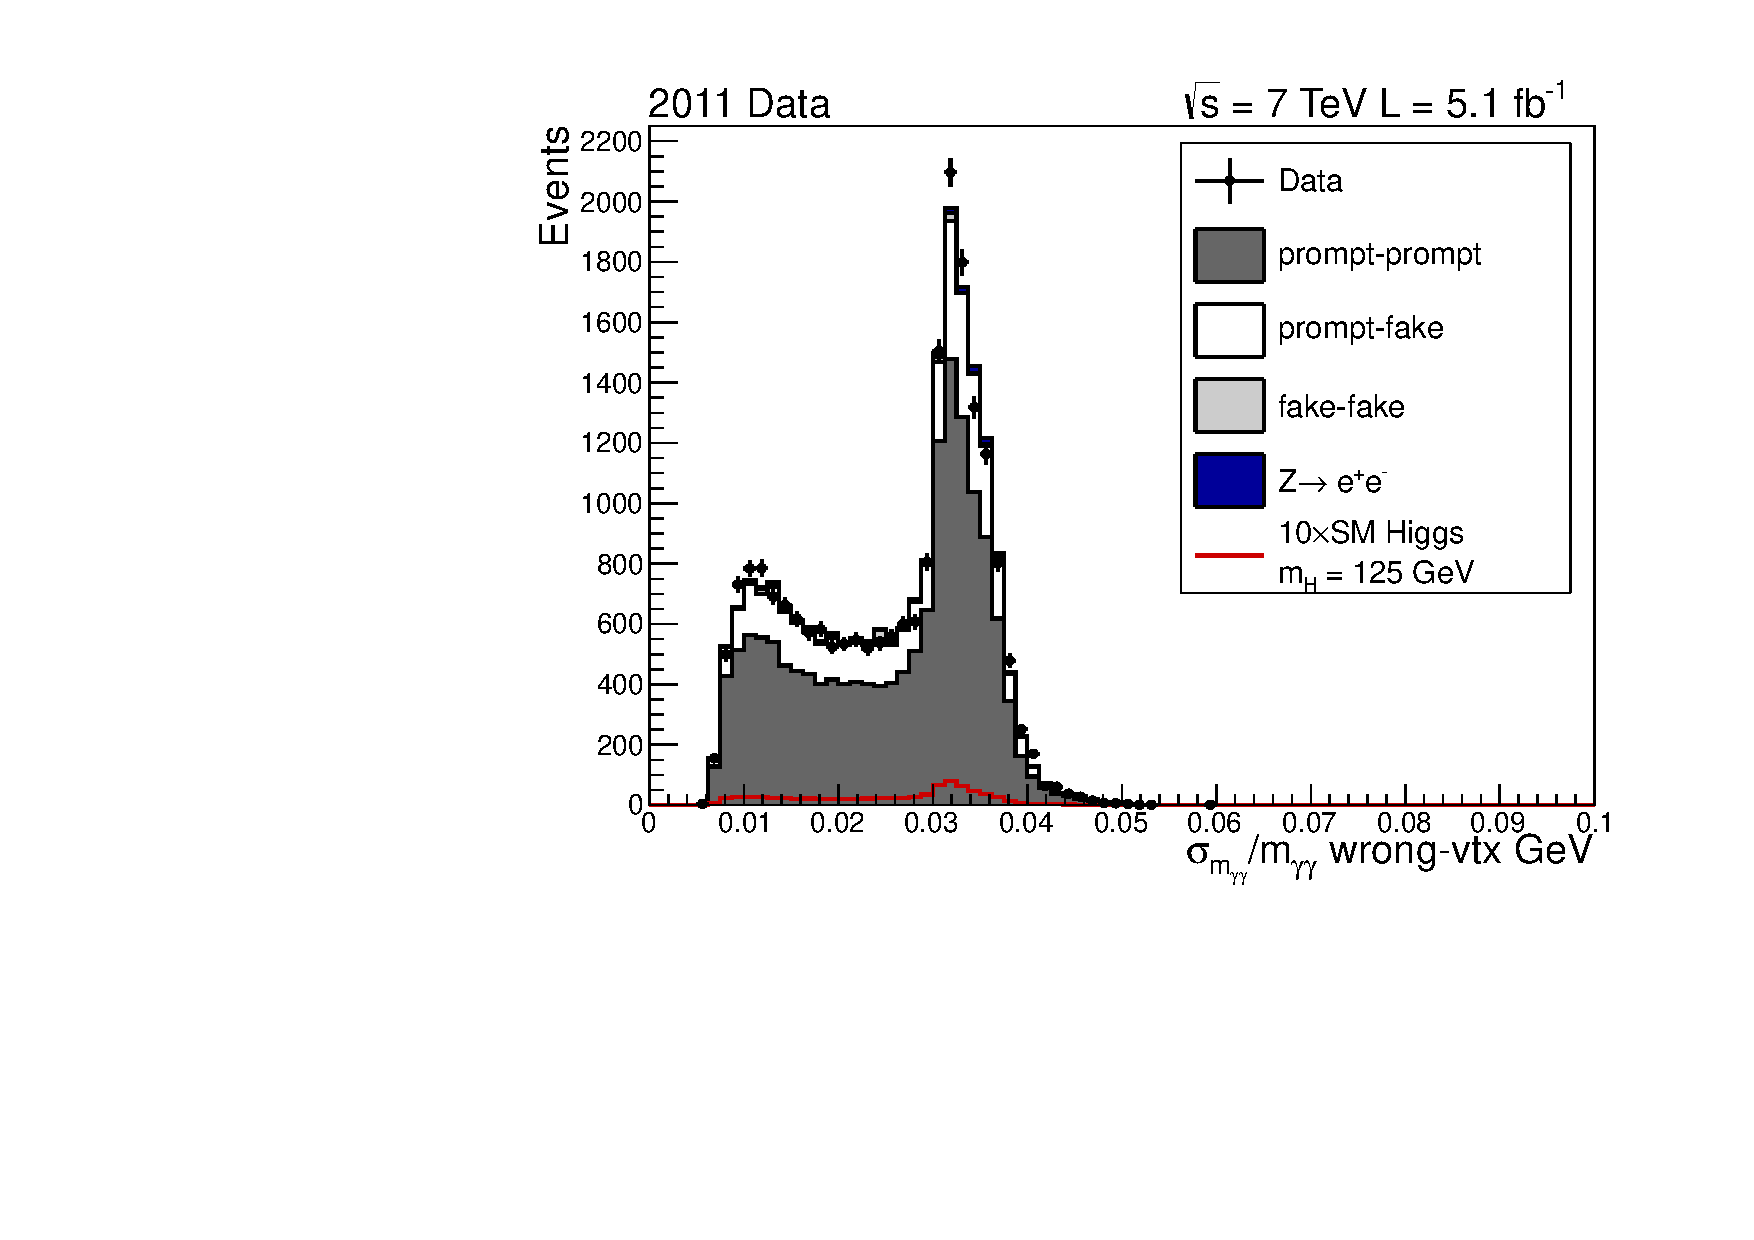
\includegraphics[width=0.48\textwidth]{hgg7TeV/variablePlots/sigmwv}
 \label{fig:diphotonbdtvars2}
 \caption{Additional diphoton BDT input variable distributions in data and MC. 
	  The distributions are for events which pass the full selection 
	  including a cut on the diphoton BDT output of 0.05.
 	  The expectation from a SM Higgs with 125 GeV is shown in red.}
\end{center}
\end{figure}

\begin{figure}[hbt!]
\begin{center}
  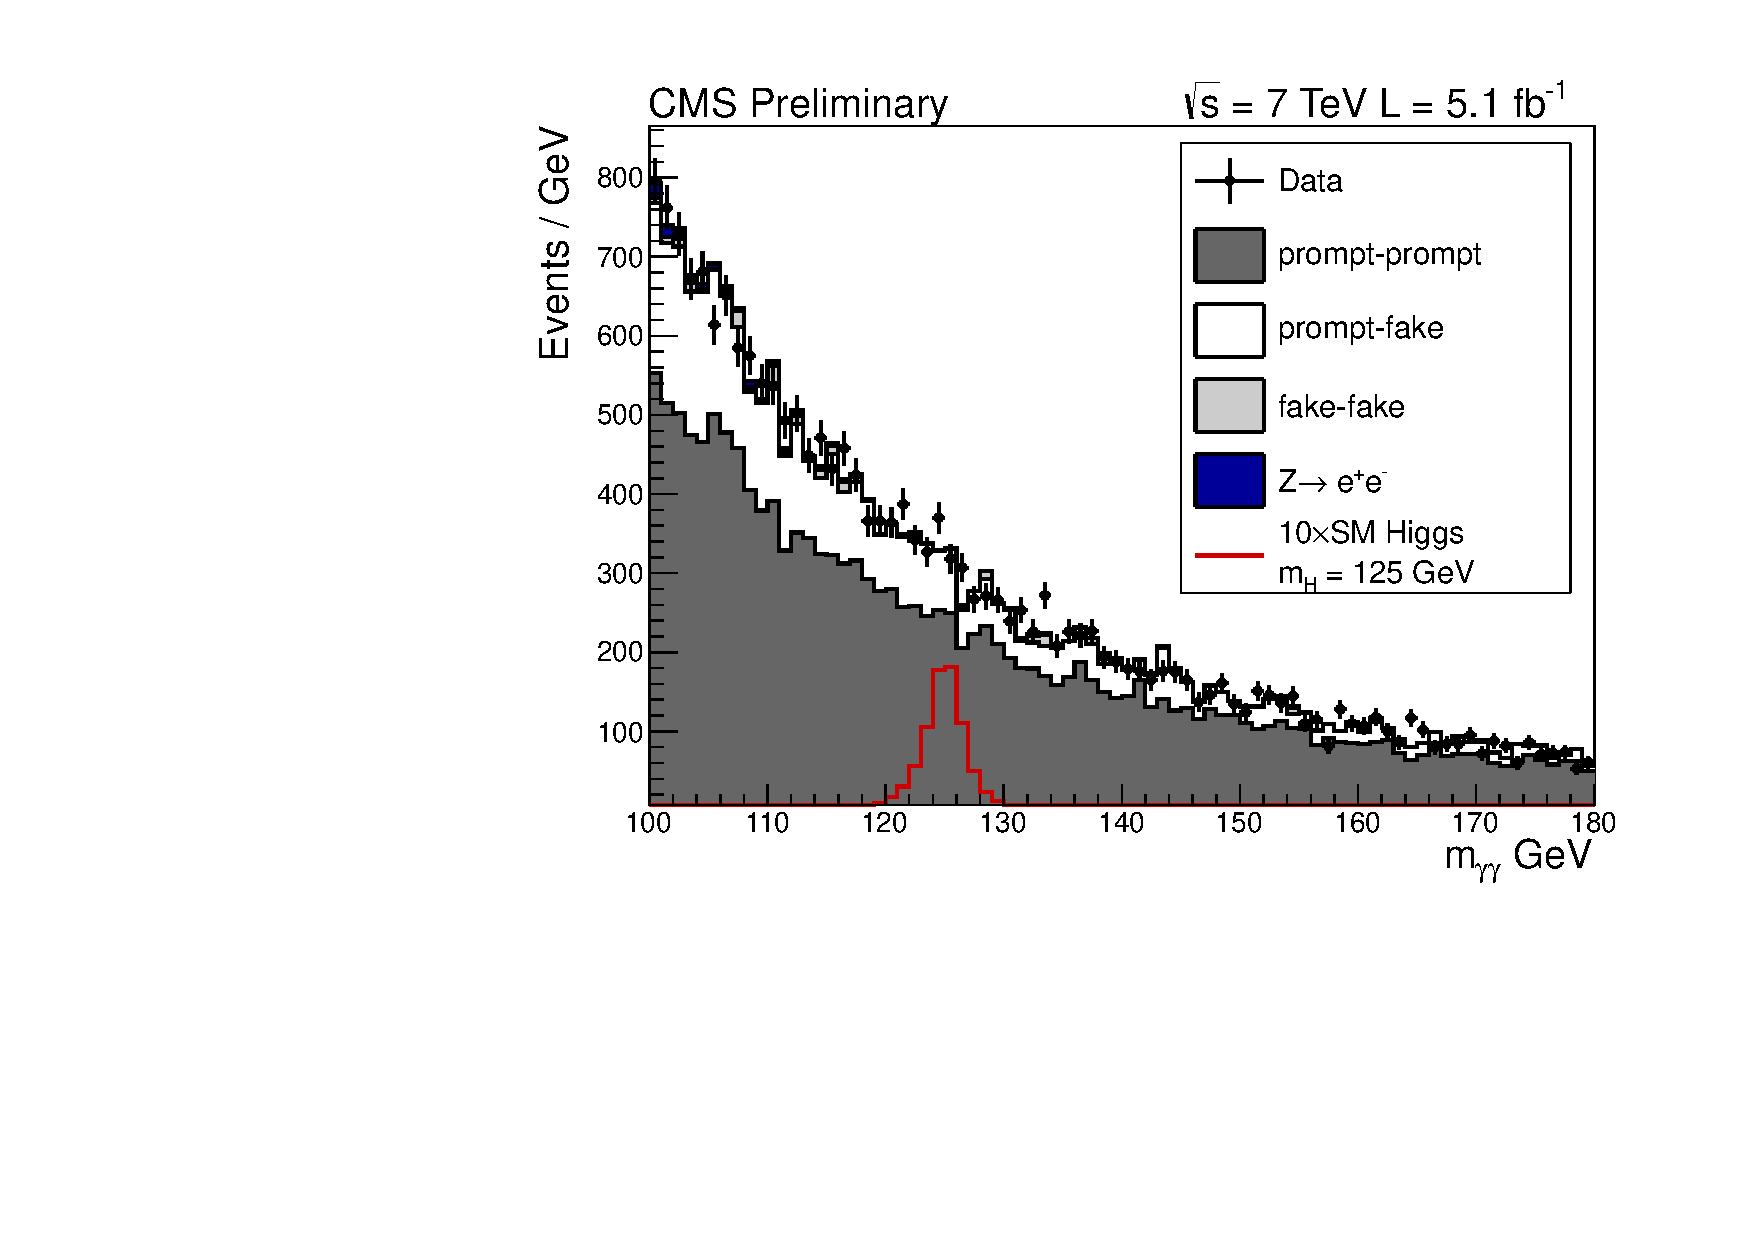
\includegraphics[width=0.8\textwidth]{hgg7TeV/variablePlots/mass}
 \caption{Invariant mass distrobution in data and MC after applying the full event selection in the
 range 100 to 180 GeV. The contribution expected from a SM Higgs with mass 125 GeV, scaled by 10, 
 is shown in red. }
 \label{fig:massmcdata}
\end{center}
\end{figure}

\subsubsection{Diphoton BDT Validation with $\Zee$ Data}
By using a BDT for the full event selection, subtle correlations between the input variables are acounted for
which improves the separation between the signal and background. 
Unlike the background model, the signal model will be taken from corrected MC simulation. 
It is important therefore to ensure that the BDT will respond in the same way in data as for the signal MC
used for the signal extraction. The MC can be validated using $\Zee$ data-MC
comparisons by inverting the electron veto and treating the electrons as though they were photons.
This is done by using the supercluster associated to the electron for the electron's energy measurement 
and ignoring the track information. In this way, the reconstruction of the electrons is the same as that
of the photons allowing for validation of the BDT's response to real photons from a resonance decay~\cite{null}. 
Figure~\ref{fig:zeevaliddiphomva} shows the diphoton BDT distribution in $\Zee$ MC and data after applying
the full selection using this technique. 

\begin{figure}
\begin{center}
  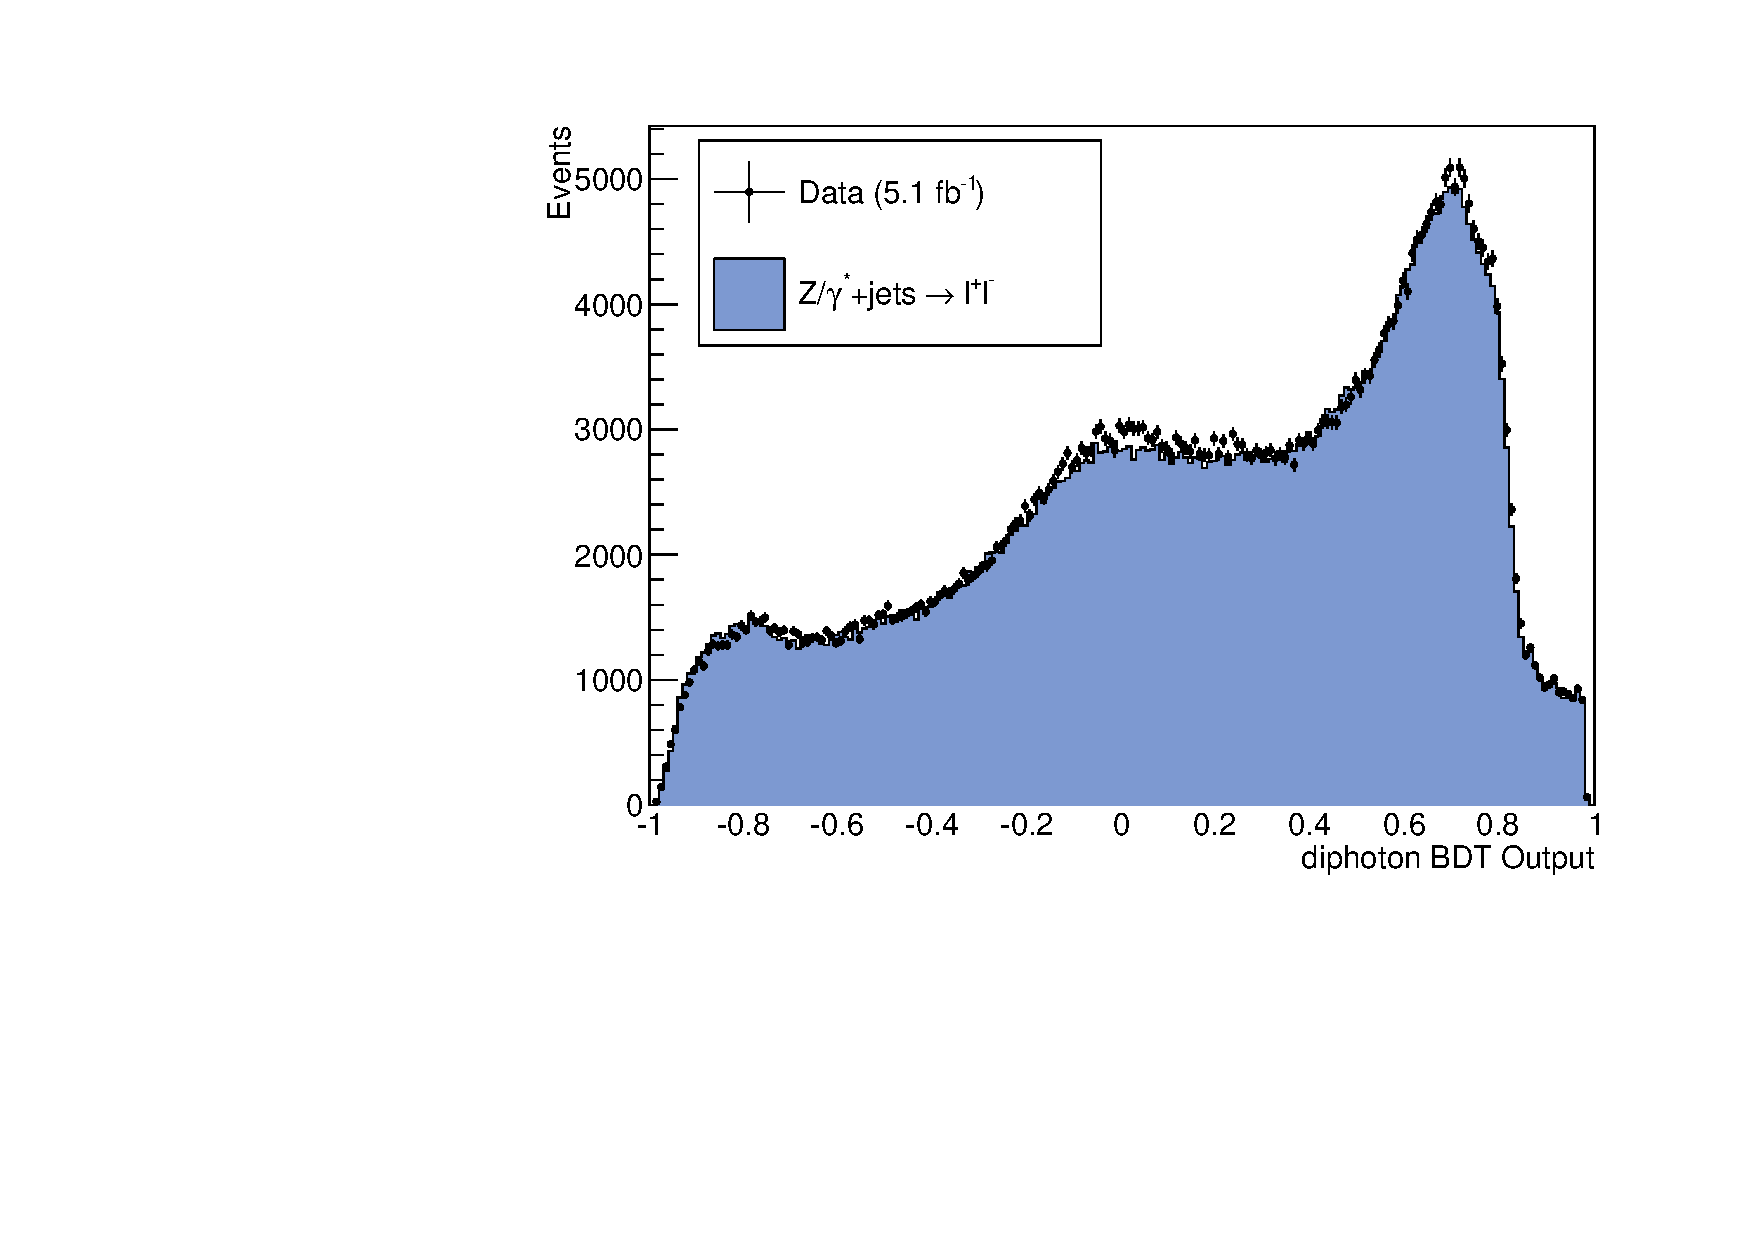
\includegraphics[width=.6\textwidth]{hgg7TeV/zeeValidation/zeevalidationdipho.pdf}
\label{fig:zeevaliddiphomva}
\caption{Diphoton BDT output distribution in $\Zee$ MC and data after the full selection 
treating the electrons as photons for the purposes of energy reconstruction. The electron 
veto is inverted to preferentially select electrons.}
\end{center}
\end{figure}

Both the photon ID and regression BDT rely on a detailed simulation of electromagnetic showering  
in MC to correctly describe the data. Due to impoerfections of this simulation, systematic
uncertainties are included in the signal model to cover the residual difference observed between MC and data
in a high $\pt$ photons. 
These uncertainties are validated using $\Zee$ in the same way as the diphoton BDT. 
Figures~\ref{fig:zeevalidsigmaE} and~\ref{fig:zeevailidphoidmva} show the distributions of the 
per photon energy resolution estimator $\sigma_{E}$ relative to the photon energy and the output of the 
photon ID BDT in $\Zee$ MC and data treating the electrons as photons. The red lines
show the $\pm 1\sigma$ error envelope attributed to the systematic uncertainty on the shower simulation.
These uncertainties are propagated through the diphoton BDT and included in the signal model as described in 
Section~\ref{sec:signalmodel}.

\begin{figure}
\begin{center}
  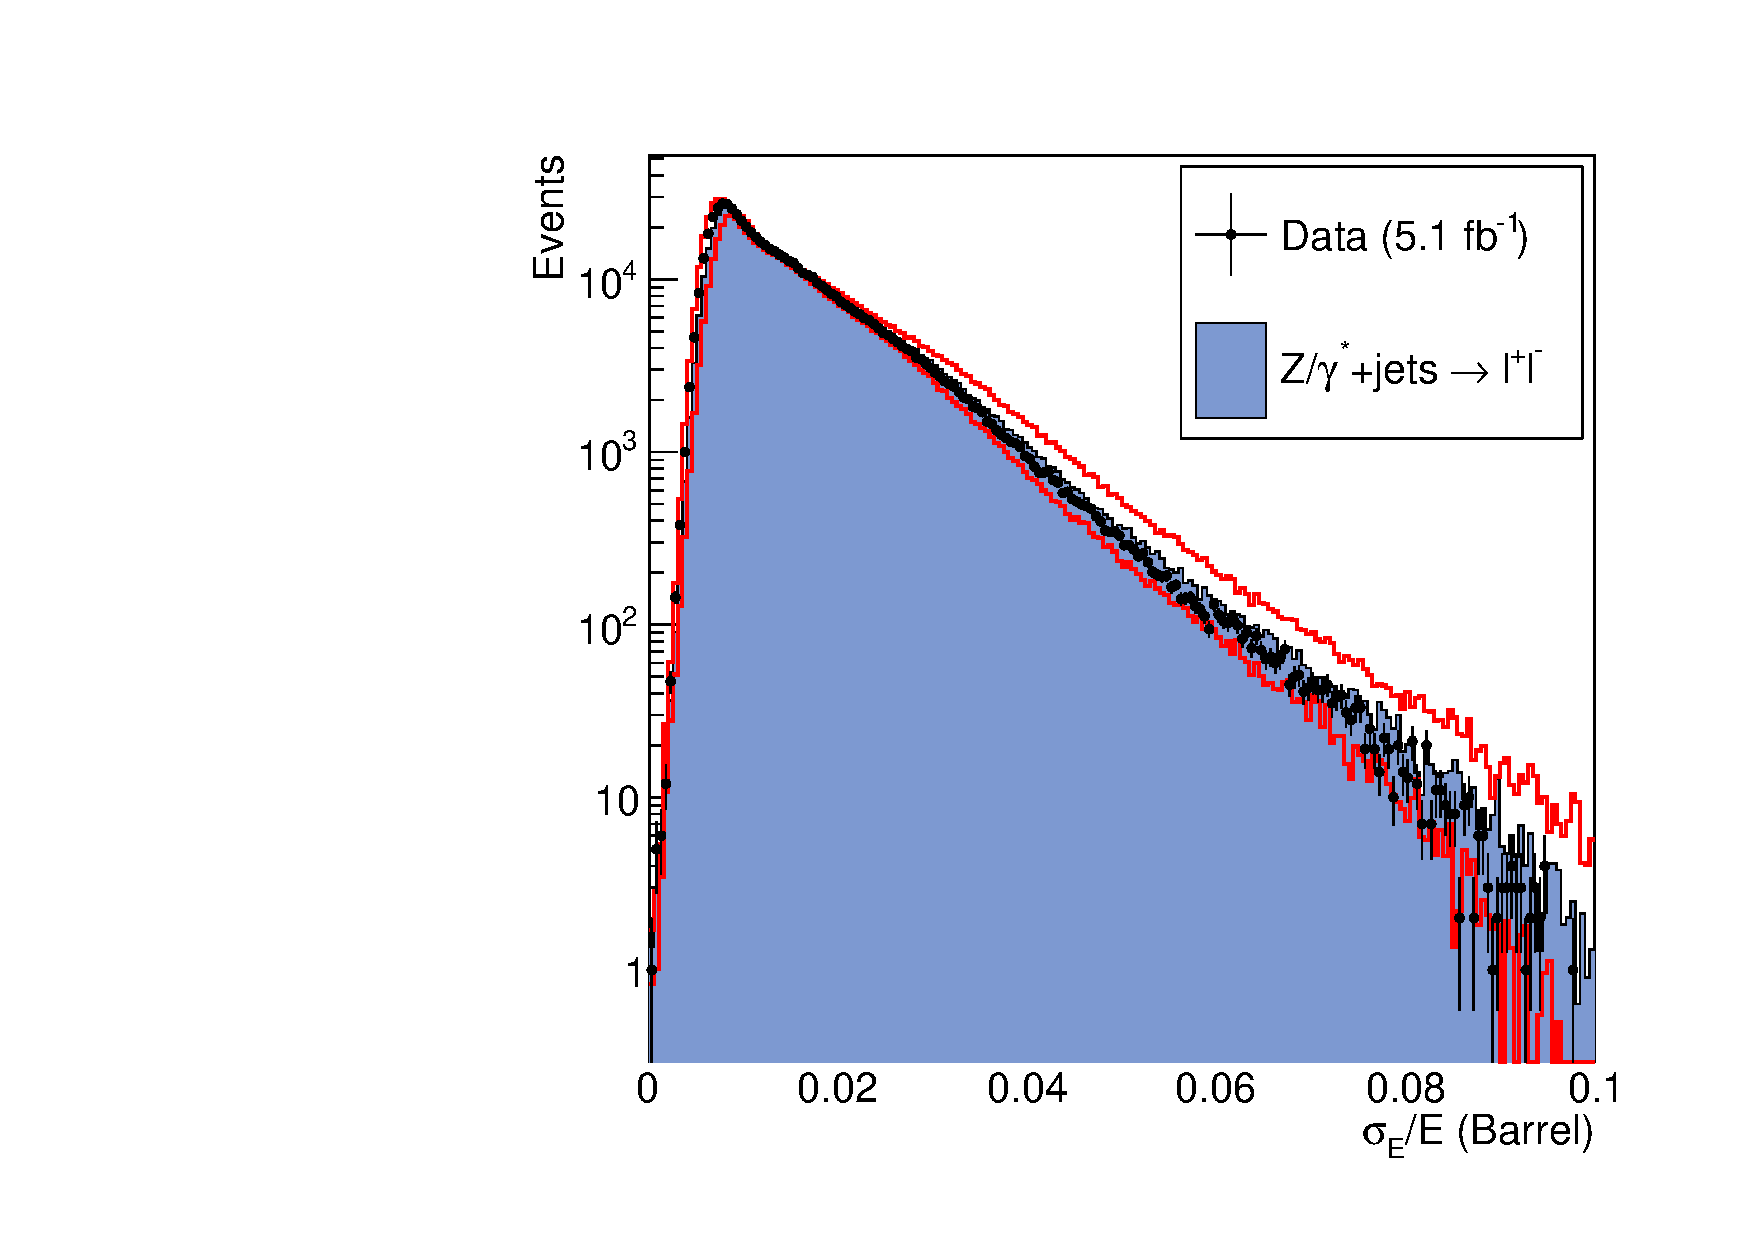
\includegraphics[width=.48\textwidth]{hgg7TeV/zeeValidation/sigmaE_EB.pdf}
  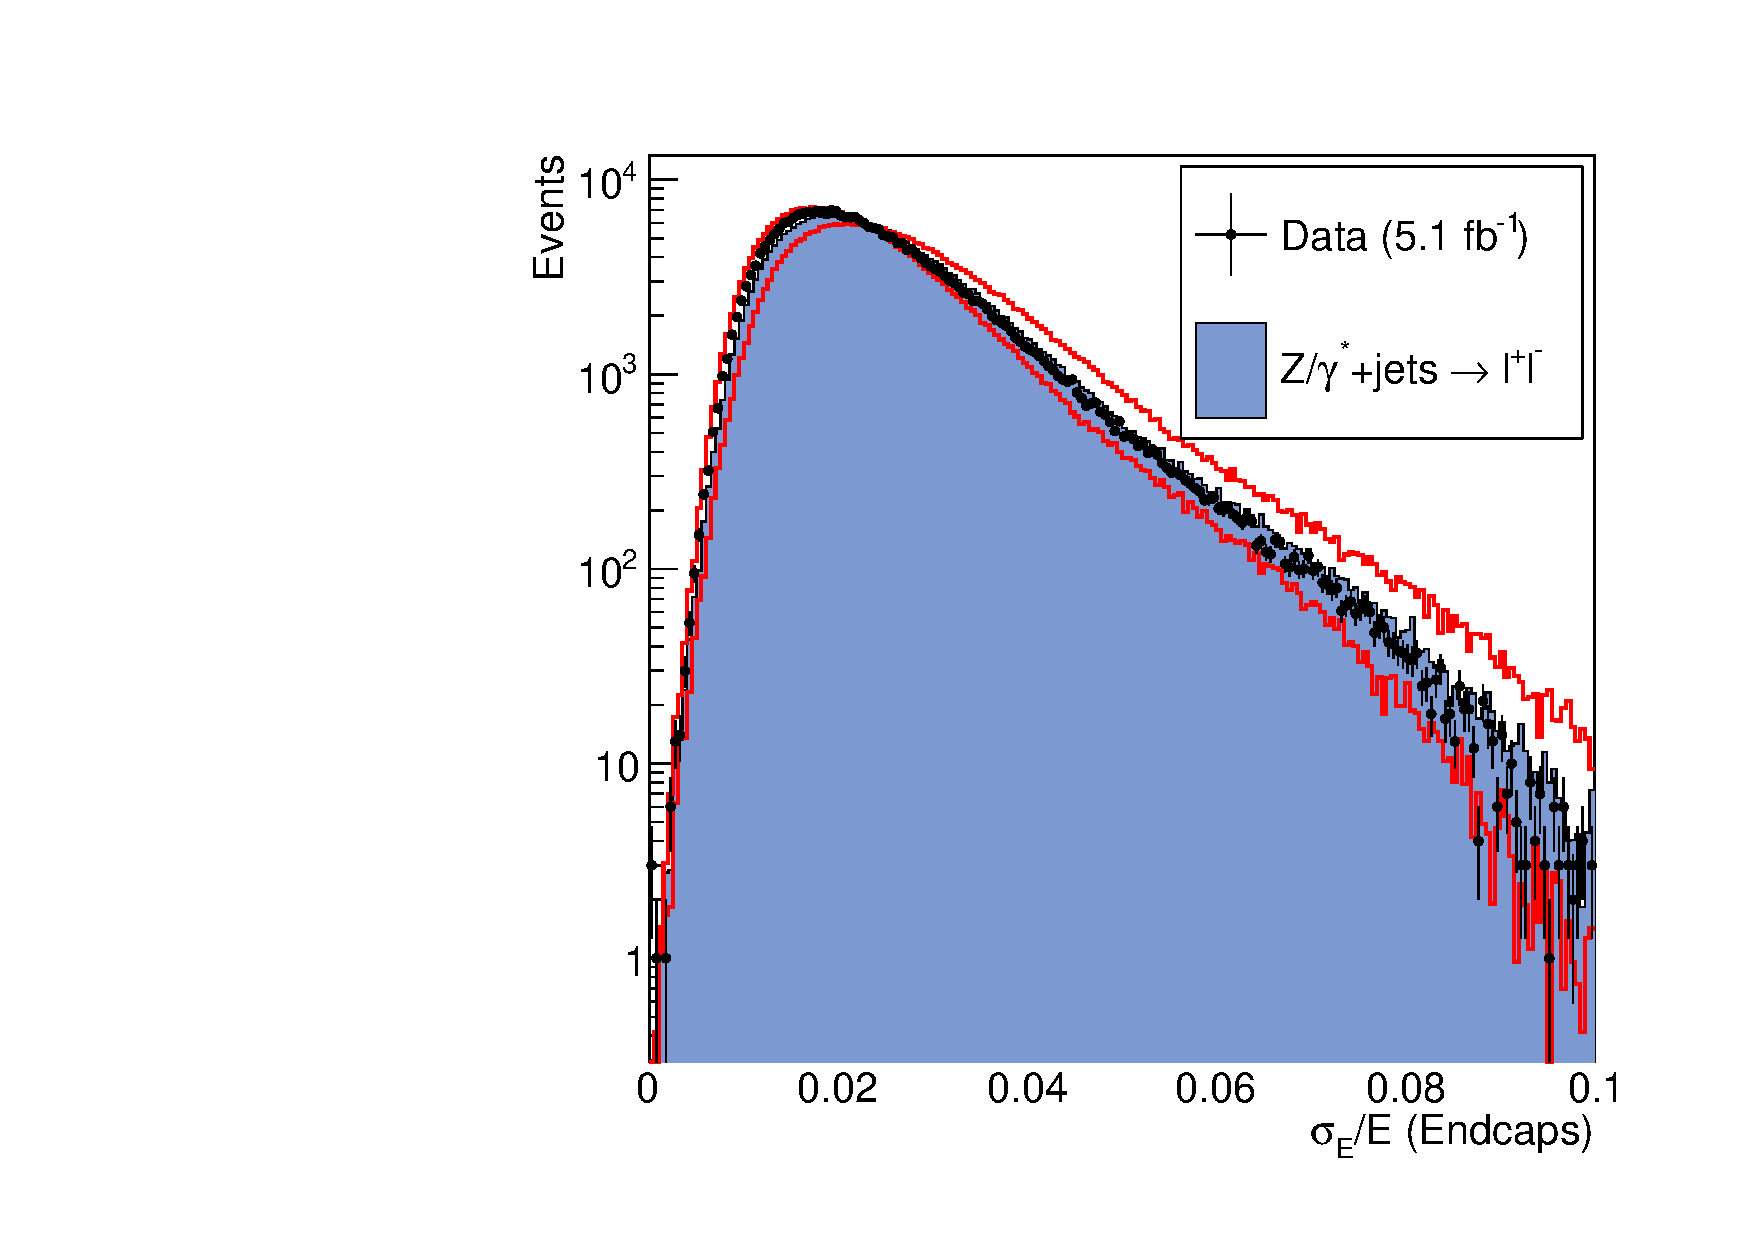
\includegraphics[width=.48\textwidth]{hgg7TeV/zeeValidation/sigmaE_EE.pdf}
\label{fig:zeevalidsigmaE}
\caption{Upper: Per-photon resolution estimator, $\sigma_{E}$ relative to the measured energy in $\Zee$ 
MC and data 
treating the electrons as photons in the barrel (left) and endcaps (right). 
The red lines show the $\pm 1\sigma$ systematic error envelope obtained by scaling the value of 
$\sigma_{E}$ by $\pm 10\%$.}
\end{center}
\end{figure}

\begin{figure}
\begin{center}
  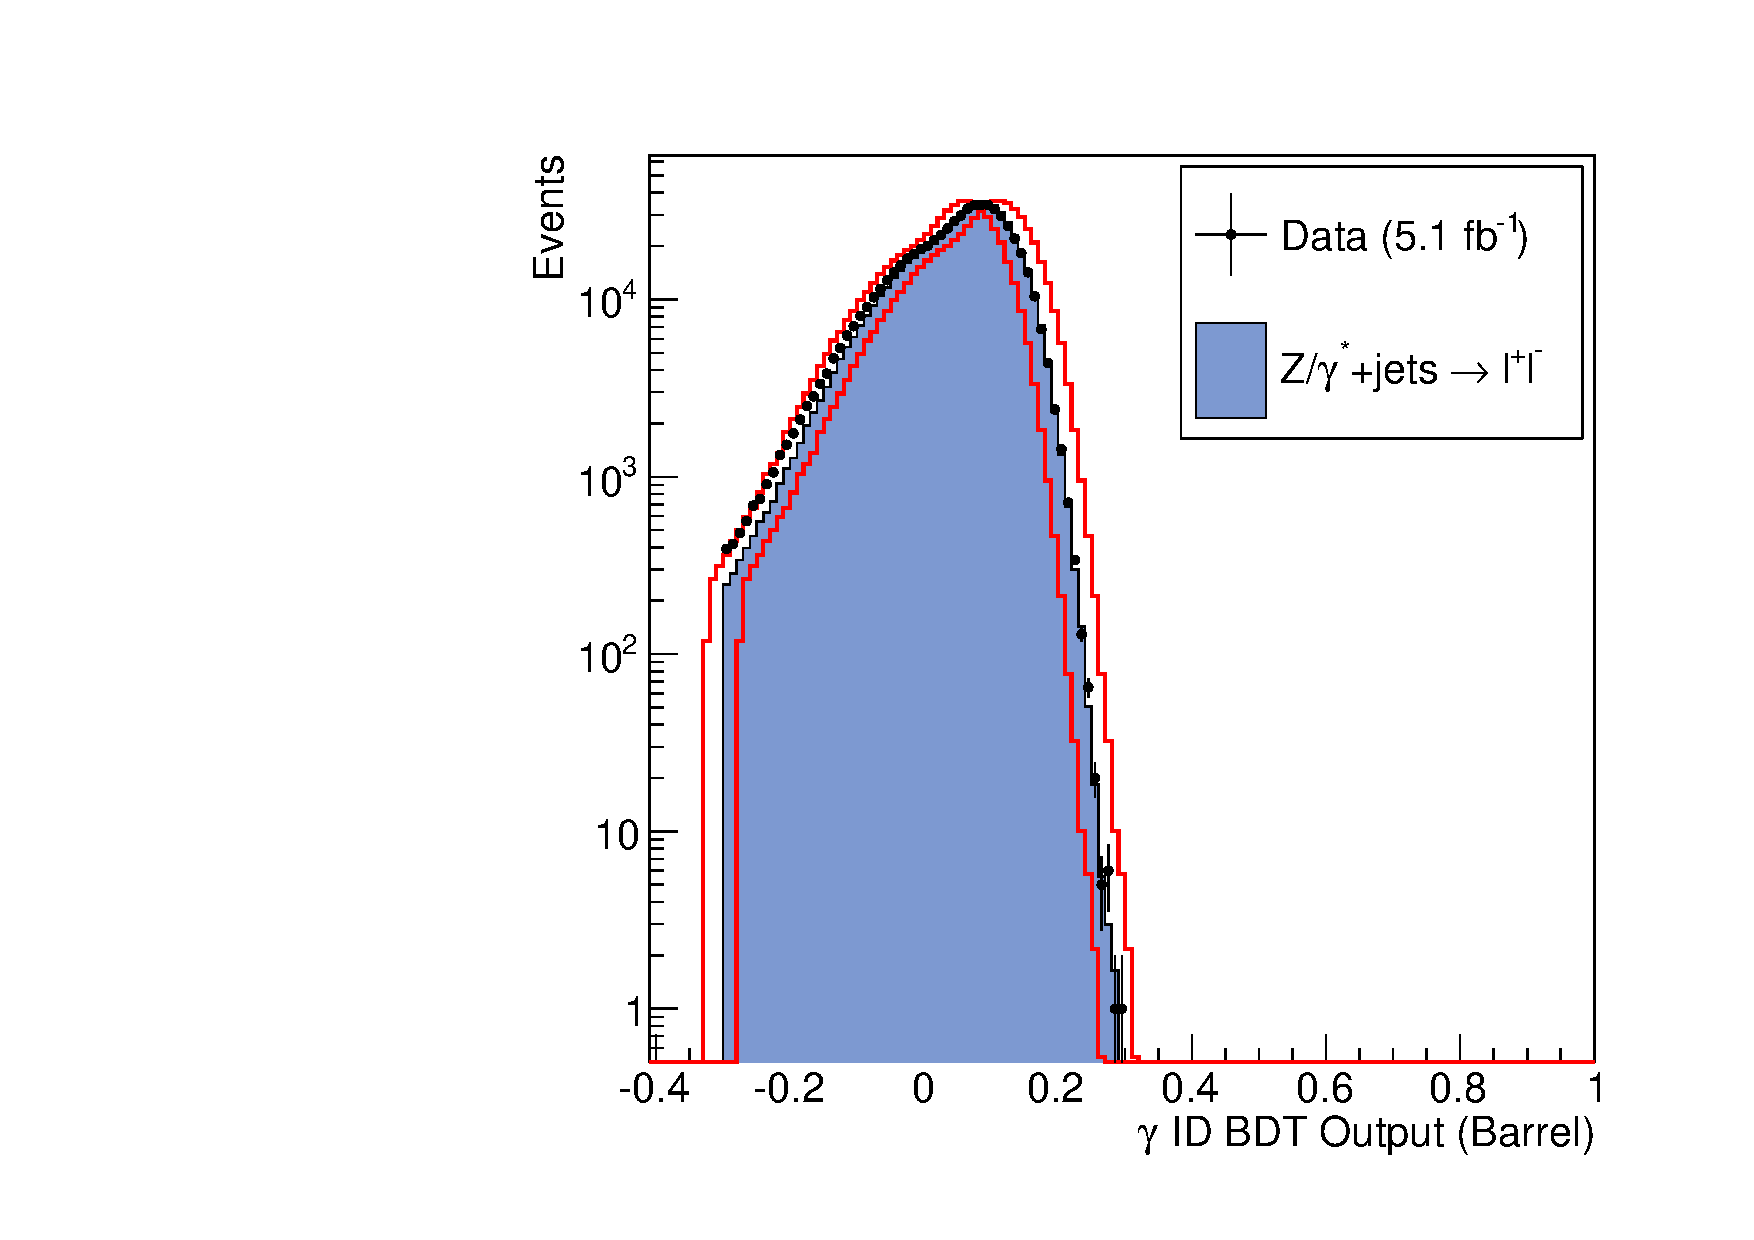
\includegraphics[width=.48\textwidth]{hgg7TeV/zeeValidation/phoID_EB.pdf}
  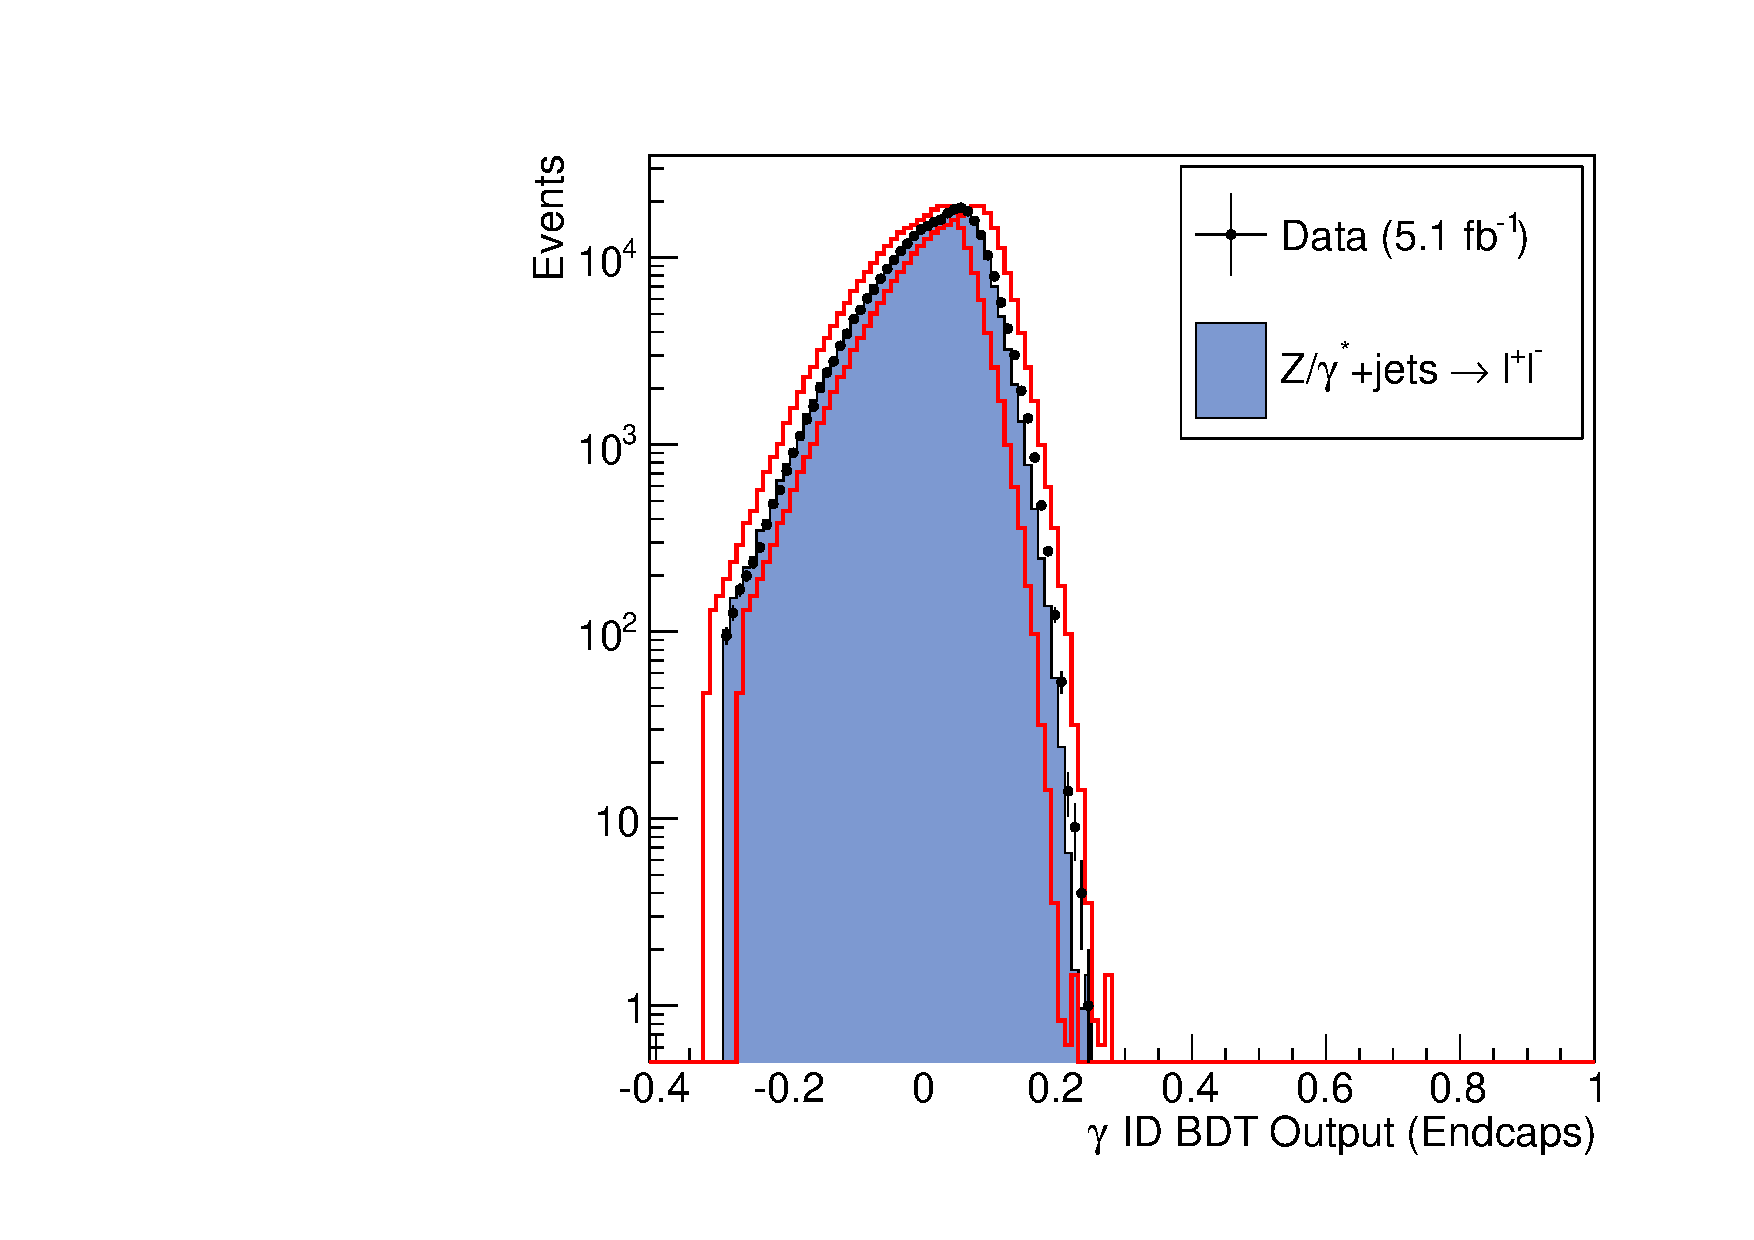
\includegraphics[width=.48\textwidth]{hgg7TeV/zeeValidation/phoID_EE.pdf}
\label{fig:zeevalidphoidmva}
\caption{Photon ID BDT output in $\Zee$ MC and data 
treating the electrons as photons in the barrel (left) and endcaps (right). 
The red lines show the $\pm 1\sigma$ systematic error envelope obtained by shifting the output value by $\sigma_{E}$ by $\pm 0.025\%$.}
\end{center}
\end{figure}


\subsection{Dijet Tagging}
\label{sec:dijettagging}

The contribution to Higgs production from vector boson fusion is around a factor ten smaller than that
of gluon-gluon fusion. However, additional information from the two jets associated 
with $qqH$ production allows for further reduction of the diphoton background~\ref{HIG-11-033}.
Events containing two jets which pass the full selection and in addition
satisfy a series of criteria designed to target the specific topology of the dijet system are 
tagged as likely to have originated from $qqH$ production. For example, Figure~\ref{fig:vbfdeta} shows the 
separation in $\eta$ between the two jets. Signal events from vector boson fusion production are
more likely to have a large separation than those from background processes. The full set of 
criteria is given in Table~\ref{tab:vbfcuts}.
The dijet tagged events are categorized separately to 
the remaining events, thereby exploiting their high signal to background ratio for the purpose of signal
extraction. 

\begin{table}
\begin{center}
\begin{tabular*}{0.5\textwidth}{@{\extracolsep{\fill}}|l|c|}
\hline
\textbf{Variable} & \textbf{Cut Value} \\
\hline
\hline
$E_{T}^{j^{1}}$ & $>$ 30 GeV \\
$E_{T}^{j^{2}}$ & $>$ 20 GeV \\
$m_{jj}$ 	 & $>$ 350 GeV \\
$|\eta_{j^{1}} - \eta_{j^{2}}|$ & $>$ 3.5 \\
$|\phi_{jj} - \phi_{\gamma\gamma}|$ & $>$ 2.6 \\
$|\frac{1}{2}(\eta_{j^{1}} + \eta_{j^{2}}) - \eta_{\gamma\gamma}|$ & $<$ 2.5 \\
\hline
\end{tabular*}
\label{tab:vbfcuts}
\caption{Dijet selection criteria for the two identified jets
to be considered likely associated to $qqH$ production. The leading and subleading $E_{T}$ jets
are denoted $j^{1}$ and $j^{2}$ respectively.}
\end{center}
\end{table}

\begin{figure}
\begin{center}
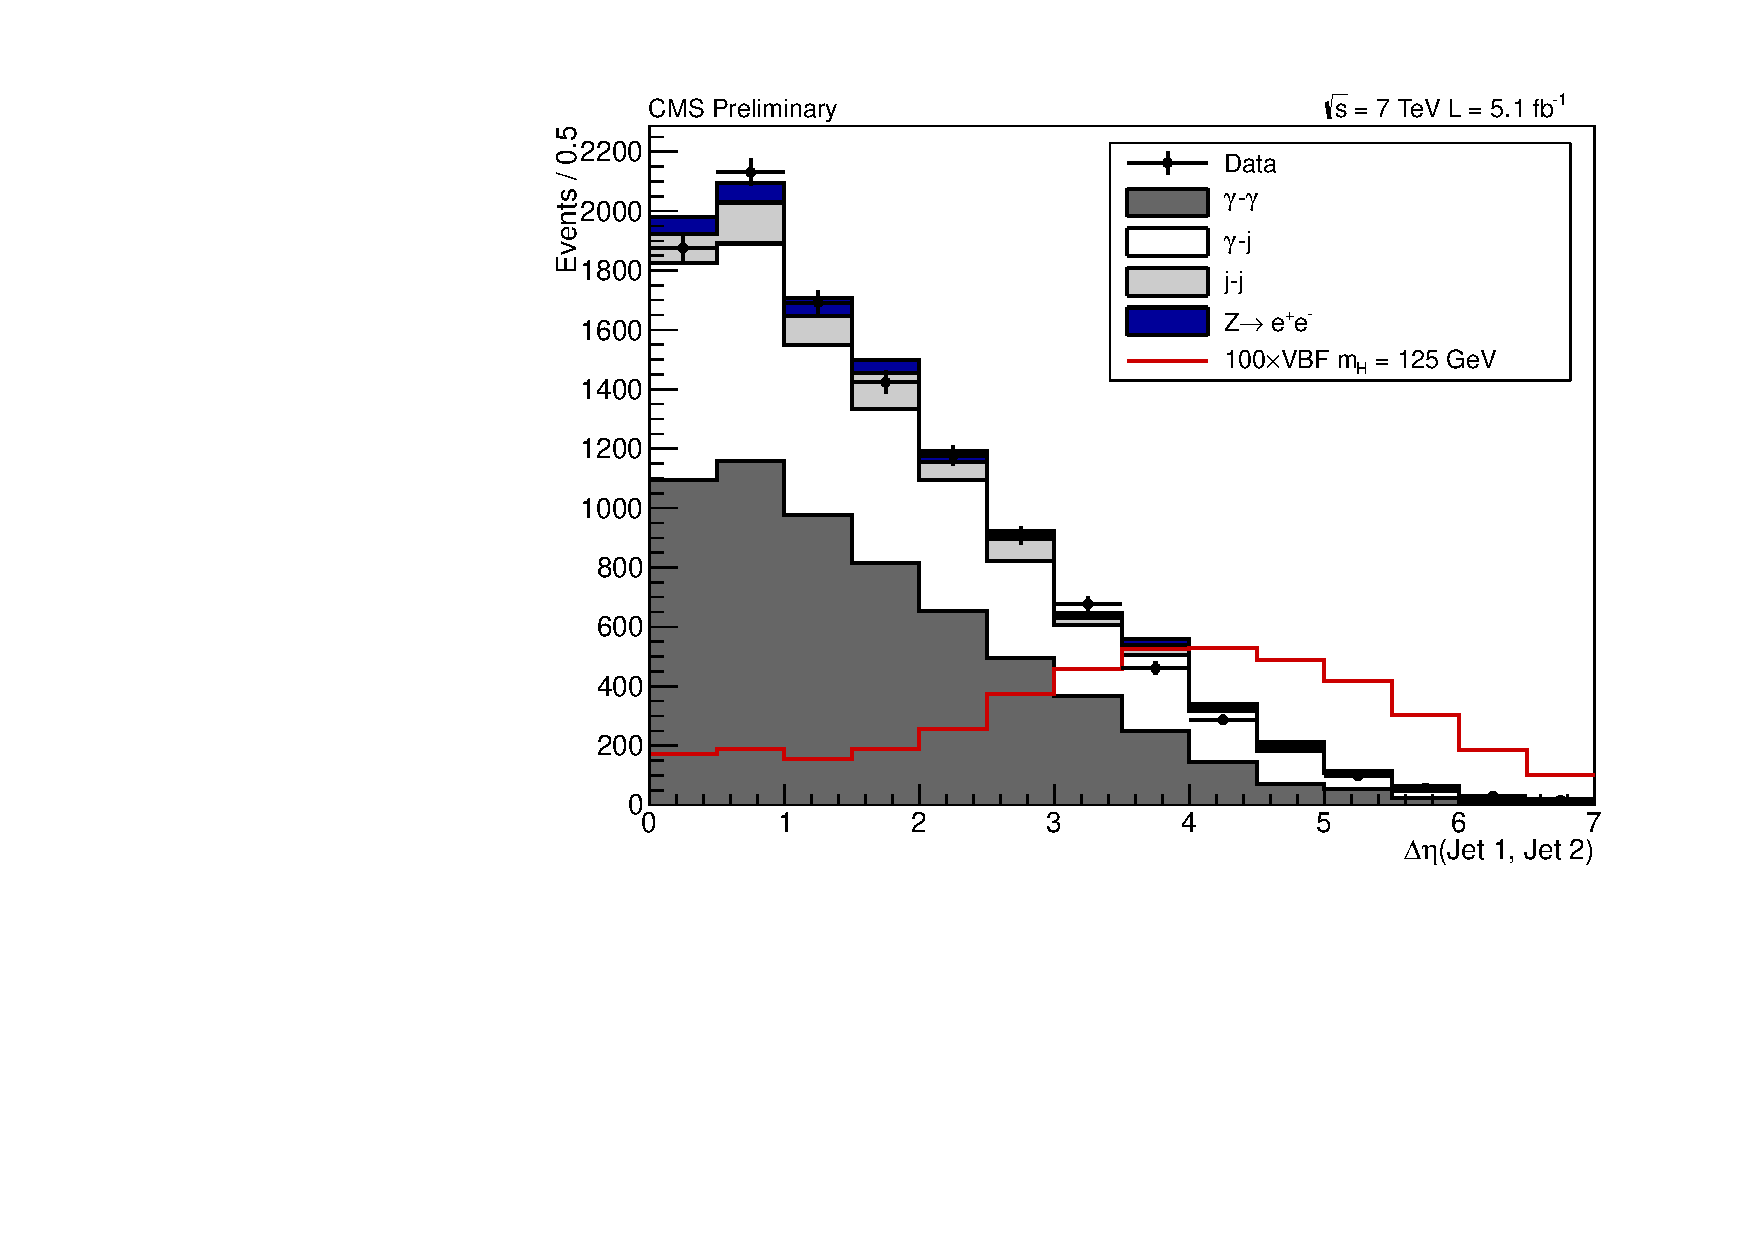
\includegraphics[width=0.8\textwidth]{hgg7TeV/variablePlots/cut_VBF_dEta_sequential_cat0.pdf}
\label{fig:vbfdeta}
\caption{Separation in $\eta$ between two identified jets in data and MC. 
The expectation from a SM Higgs produced via vector boson fusion ($qqH$), scaled by 100,
is shown in red. All cuts other than the one on $\Delta\eta(Jet 1, Jet2)$ are applied to these distributions.} 
\end{center}
\end{figure}


	\section{Signal Extraction}
\label{sec:signalextraction}
The signature for the decay $\Hgg$ is the presence of a narrow peak on a smoothly falling background in 
the invariant mass spectrum. 
The signal to background ratio can be dramatically increased by focusing on events falling in a window 
around the mass of the Higgs boson, $m_{H}$. Since this mass is not predicted in the Standard Model, 
the search is performed for a range of mass hypotheses effectively sliding the signal window across 
the diphoton invariant mass spectrum, $\mgg$.
As the signal yield for a SM Higgs boson decaying to two photons is small, 
additional event information from the detector and the kinematics of the diphoton system can be used to 
increase the sensitivity of the search. 

This section describes a multivariate analysis (MVA) based approach to extracting the signal, categorizing events within a sliding 
signal window based on a single event discriminator (categorisation BDT). The approach allows for use of data in sidebands
to determine expected event yields within the signal region, making few assumptions about the specific
composition and kinematics of the background. This approach is the second of the two methods (method B) for extracting the signal, used by the CMS $\Hgg$ group.

\subsection{Definition of the Signal Region}

Once the expected resolution of the $\Hgg$ peak is determined, the choice of signal window can be optimized
to reduce the uncertainty on the background while selecting as many signal events as possible.
The size of the signal window is chosen using a simplified analysis in which the number of signal events
from a SM Higgs boson with hypothesised mass $m_{H}$ expected within the range $|\Delta M/M_{H}|=|(\mgg-m_{H})/m_{H}| < w$ 
is compared to the uncertainty on the total number of events (from background and signal) in that range.
The figure of merit, $N_{S}/\sigma = N_{S}/\sqrt{\sigma_{S}^{2} + \sigma_{B}^{2}}$, is calculated as
a function of signal region cut value, $w$, for a range of mass hypotheses as shown in Figure~\ref{fig:sigwindowopt}. 
The error on the number of background events, $\sigma_{B}$, is calculated using the procedure described in 
Section~\ref{sec:backgroundmodel} whereas the error on the signal is purely statistical.
For this analysis, $w=0.02$ was chosen as the optimal signal region cut value.

\begin{figure}
 \begin{center}
  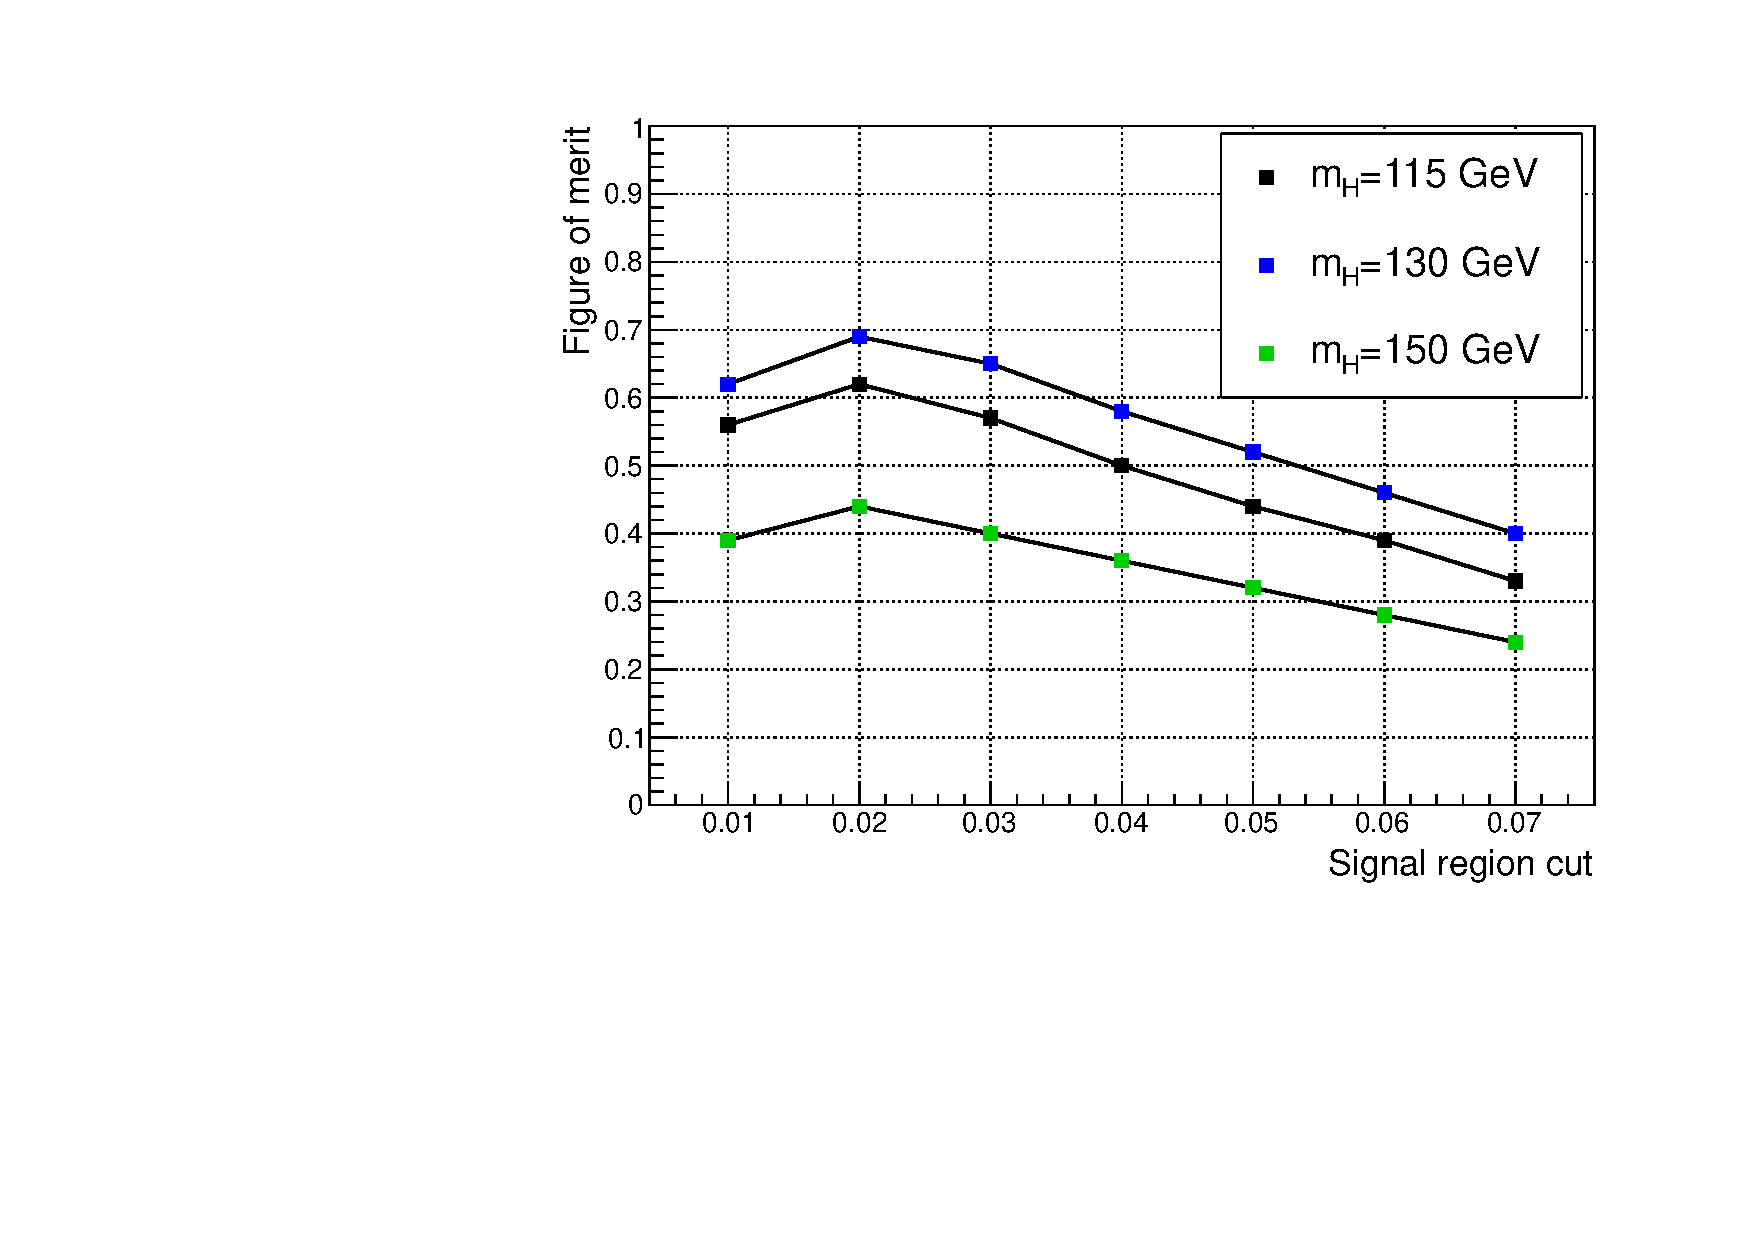
\includegraphics[width=0.9\textwidth]{hgg7TeV/sidebandMvaPlots/fom.pdf}
 \end{center}
  \caption{Figure of merit for selection of the signal region cut value, $w$. Each colour shows the evaluation
  under different Higgs boson mass hypotheses.}
  \label{fig:sigwindowopt}
\end{figure}


\subsection{Event Categorisation BDT}
\label{sec:bdteventdiscriminator}

The inputs to the diphoton BDT contain information from the event kinematics and the quality of the photons 
and vertex location in the form of the photon ID BDT output and event resolution estimators. 
The output of the diphoton BDT combined with the invariant mass of the diphoton system therefore provides 
the necessary information to separate signal from background.

Figure~\ref{fig:bdtplane} 
shows the variation in the signal to background ratio ($S/B$) across different regions in the 
two-dimensional plane defined by the output of the diphoton BDT and $\dmom$.
Events close to the centre of the peak ($\dmom=0$) with a high score in the diphoton BDT are more
likely signal events than those far from the high $S/B$ regions.

\begin{figure}
\begin{center}
  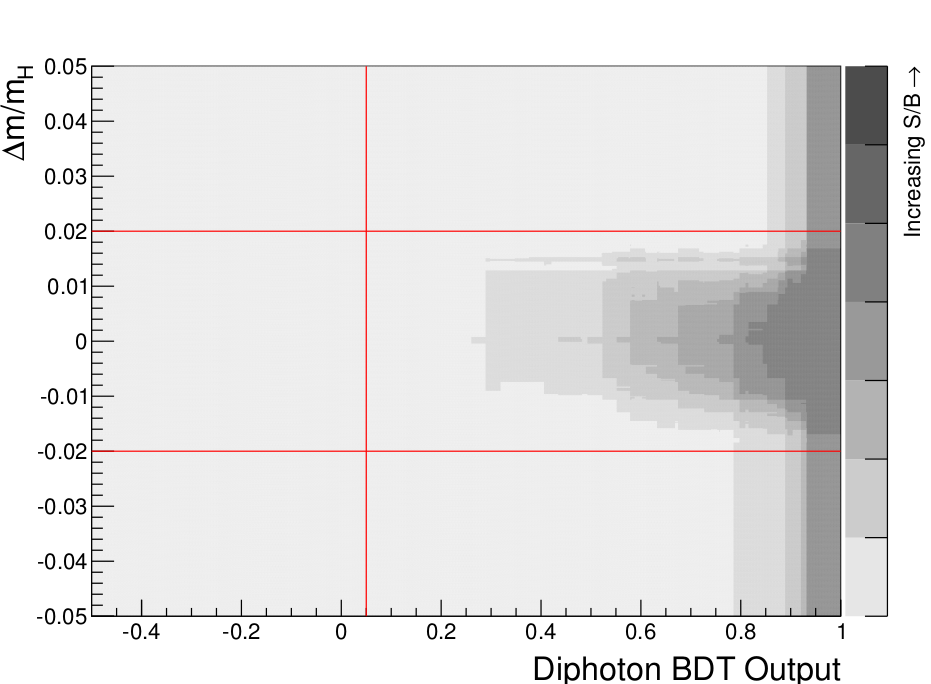
\includegraphics[width=0.8\textwidth]{hgg7TeV/sidebandMvaPlots/bdt2dplot.png}
\end{center}
 \caption{Signal to background ratio as a function of diphoton BDT output and $\dmom$.
 The red lines indicate the cuts applied before the training and for applying the event selection. 
Darker shades indicate a regions with a higher signal to background ratio. The seven shades indicate the 
region contained in each of the seven BDT bins used for the signal extraction at $m_{H}= 123$ GeV.}
 \label{fig:bdtplane}
\end{figure}

The two variables are combined to produce a single event discriminator by training a BDT using the 
diphoton BDT output and $\dmom$ as inputs. 
The BDT is trained with Higgs signal MC with $m_{H}=123$ GeV including all four production processes 
and background MC including prompt-prompt, prompt-fake and fake-fake events.
The performance of several different training methodologies was compared to find which gave the 
optimum separation of signal and background.
Two different choices of boosting were studied, adaptive and gradient boosting, both of which 
weight decision trees to optimize the performance in terms of signal-background separation~\citep{tmva}. 
In addition, these were compared to a simple likelihood 
which does not account for correlations between the 
diphoton BDT and $\dmom$ as shown in Figure~\ref{fig:mvacomparisons}.
The gradient boosting method was found to give the best performance although the variation between 
methodologies is small.
 
\begin{figure}
\begin{center}
  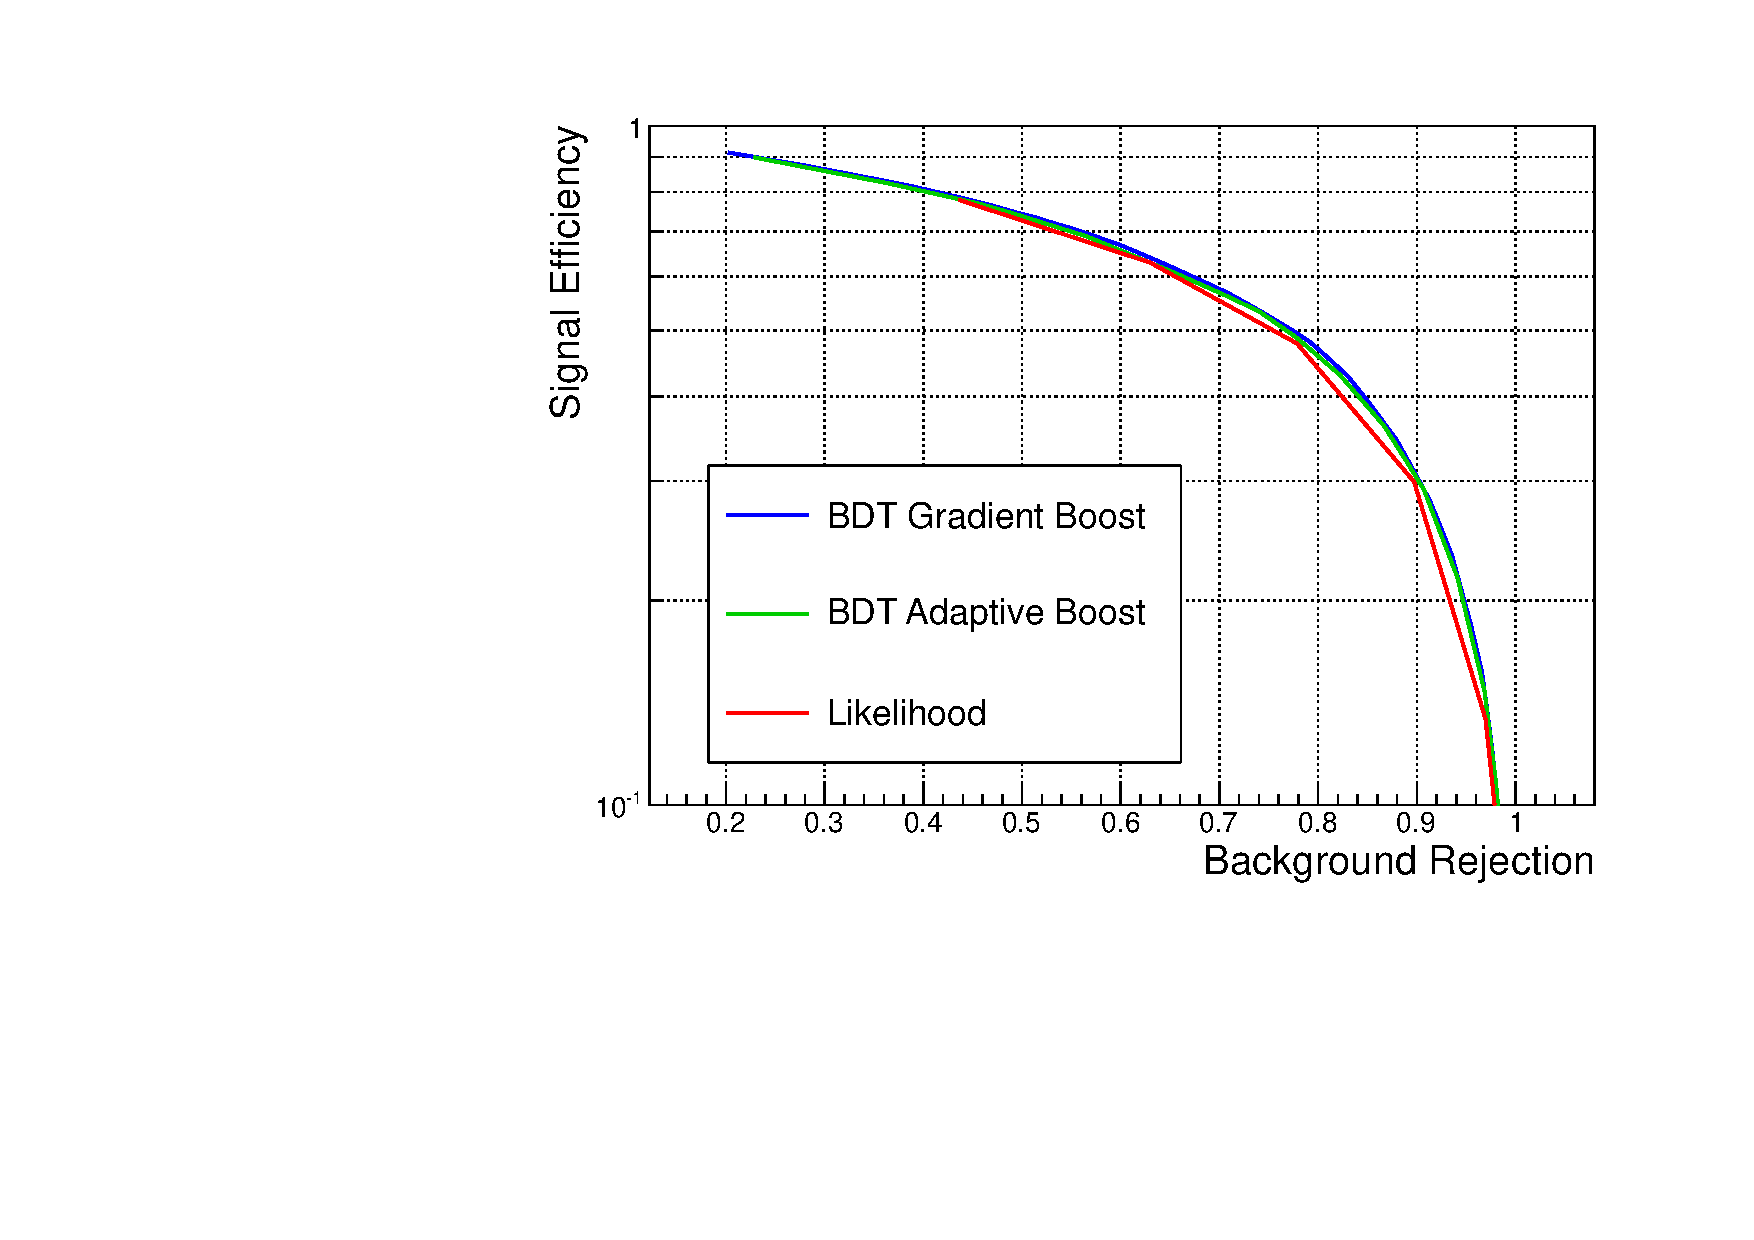
\includegraphics[width=0.8\textwidth]{hgg7TeV/sidebandMvaPlots/roc}
\end{center}
 \caption{Signal efficiency vs background rejection curves for three different MVA techniques used to train
 the signal-background event discriminator. The curves give the (in)efficiencies for signal (background) 
 after applying sequentially tighter cuts on the discriminator output.}
 \label{fig:mvacomparisons}
\end{figure}

With finite statistics, a BDT can be over-trained by allowing the training to emphasise statistical fluctuations which are not physical and will not necessarily be
representative of the data. To test for this, the MC samples are split into two equal samples, the first of which is used to train the BDT. The distribution 
of the output values of the BDT from the second set is compared to that of the training sample as shown in Figure~\ref{fig:bdttraining}. The comparison
is shown using both an arbitrary binning scheme and the final set of bins derived in 
Section~\ref{sec:binningofthebdtoutputdistribution}.
A $\chi^{2}$ test was performed on the distributions with the final bins giving p-values of 0.06
for the background and 0.95 for the signal indicating that over-training has not occurred.

\begin{figure}
\begin{center}
  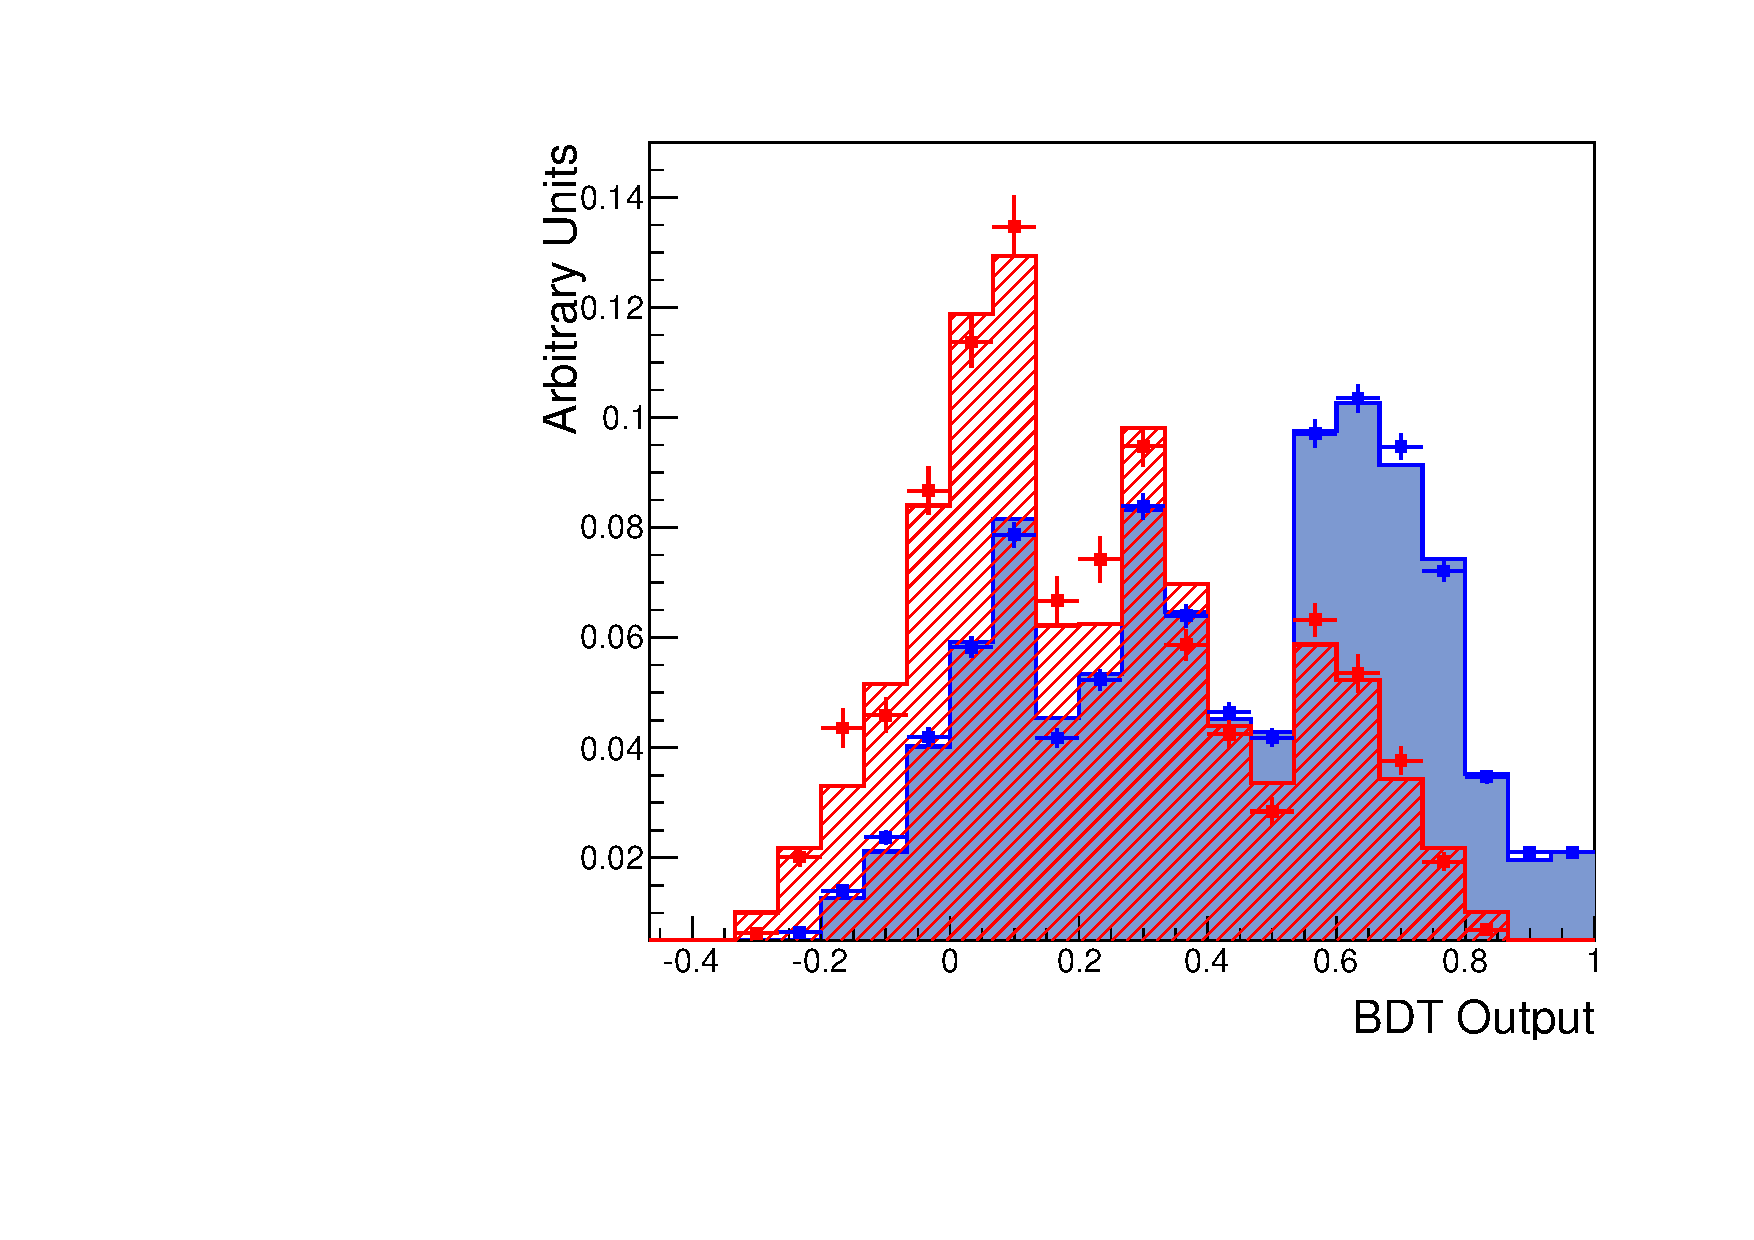
\includegraphics[width=0.48\textwidth]{hgg7TeV/sidebandMvaPlots/testvstrain_nolegend}
  \includegraphics[width=0.48\textwidth]{hgg7TeV/sidebandMvaPlots/testvstrain-finalbins-neat}
\end{center}
 \caption{Signal and background BDT output distribution with the training sample (points)
and testing sample (solid area) superimposed. The comparison is shown 
using an arbitrary uniform binning (left) and the bins used for extracting the signal (right).}
 \label{fig:bdttraining}
\end{figure}

In this analysis, the background is estimated entirely from data. This means that disagreement between
data and background MC will affect the performance of the BDT rather than the validity of the final results. 
The agreement between the data and MC is shown in Figure~\ref{fig:datamcagreement_sidebandBDT} for the mass 
hypothesis, $m_{H}=125$ GeV. The level of agreement is sufficient so as not to require in-depth study of the
BDT output distributions of the background MC.

\begin{figure}
 \begin{center}
  \includegraphics[width=.8\textwidth]{hgg7TeV/sidebandMvaPlots/data-mc-sbsum-mh125}
 \end{center}
 \caption{Comparison of the distributions of BDT output at $m_{H}=125$ GeV for data and background MC. 
 The distributions are arbitrarily binned for the purposes of comparison only.}
 \label{fig:datamcagreement_sidebandBDT}
\end{figure}

\subsection{Binning of the BDT Output Distribution}
\label{sec:binningofthebdtoutputdistribution}

The BDT provides a single variable with which to classify events based on their signal to background 
ratio, $S/B$, which will have a discrete number of response values based on the number of
trees used. The boosting procedure provides a pseudo-continuous distribution which is used
to model the signal and background. However, the resulting distribution will still be only
pseudo-continuous. In addition, the BDT response does not directly correspond to a physical
distribution and it is therefore difficult to motivate any parameterisation of either the signal
or background distributions. To overcome these issues, a binning procedure is defined to 
construct templates which are used as models for the signal and background expectation as a
function of BDT response range (BDT bin). This procedure is designed firstly to ensure that no
bin has zero background expectation and secondly that as few bins as possible
are used without reducing the sensitivity of the BDT. 
These requirements are desirable such that 
the expected background yield in each bin can be derived using data outside of the signal region
as described in Section~\ref{sec:backgroundmodel}.

A scan is performed in which the definitions of the bin boundaries are varied in order to
find the maximum expected significance in the presence of a SM Higgs signal. For $N$ bins 
($N-1$ boundaries) with background and signal expectation yields $b_{i}$ and $s_{i}$ respectively,
the expected significance, $\sigma_{exp}$, is given by

\begin{equation}
 \sigma_{exp} = \left( 2 \sum_{i=1}^{N} (s_{i}+b_{i})\ln\left(\frac{\displaystyle s_{i}}{\displaystyle b_{i}} +1\right) - s_{i} \right)^{1/2},
\label{eqn:expectedsig_bins}
\end{equation}
using the log-likelihood ratio for Poisson likelihoods.
The binning procedure is defined as follows:

\begin{enumerate}

\item The distribution of background MC is binned very finely to provide an almost discrete
dataset (5000 equally spaced bins are used). The background is re-binned such that there are 20
expected events per bin at a luminosity of \clumi. 
\item Smoothed versions of the signal (at each 5 GeV step mass) and background MC templates are produced 
in order to obtain a stable model of $S/B$ as a function of BDT bin.
The smoothing procedure is done via binning a fit (of a 9th order polynomial) to the signal
distribution.
\item $N$ bin edges (boundaries), $b_{i}$, are defined on the remaining bins such that $N+1$ bins 
are formed with $b_{1} < b_{2} < \ldots < b_{N}$. The first bin is defined as $[-1,b_{1})$ and the last
is defined as $[b_{N},1]$. The $N$ dimensional scan is performed varying these
bin edges to find the maximum expected significance in the presence of a SM Higgs signal. 
\item An extra boundary is added, the scan is repeated and the maximum expected
significance is found for $N+1$ boundaries. If the maximum expected significance  
is increased by more than 0.1\% compared to that of step 3, the new boundary is kept and step 4 
is repeated, if not, the procedure terminates.
\end{enumerate}

The scan in step 3 is split into two parts, first using a large step size to find the 
region where the maximum lies followed by a fine scan in small steps within that region. 
The ratio of small to large step size is chosen to be that
which minimizes the total number of iterations in the scan to reduce the time taken for the procedure.
An example of the binning procedure is shown in Figure~\ref{fig:binningscheme}. 
The red histogram is the $S/B$ distribution after step 1, the 
blue after step 2 and the black vertical lines show the final set of 7 bins chosen for this analysis.
Dijet tagged events are treated in the same way as the rest of the events in the analysis 
by introducing an eighth bin containing events from any BDT output bin inside the range $\dmom < w$ 
which pass the dijet tag.

\begin{figure}
 \begin{center}
  \includegraphics[width=0.8\textwidth]{hgg7TeV/sidebandMvaPlots/binningscheme.pdf}
 \end{center}
 \caption{Signal to background ratio as a function of BDT output bin.
 The red and blue histograms show the distribution after applying step 1 of the binning procedure before
and after smoothing respectively. The black vertical lines indicate the boundaries of the final
binning choice from the full procedure.}
 \label{fig:binningscheme}
\end{figure}


\subsection{Background Model}
\label{sec:backgroundmodel}

The SM background is expected to have a smoothly varying invariant mass spectrum.
However, detector effects such as selection, trigger efficiencies and energy resolution 
shape this distribution in ways which are imperfectly modelled in MC simulation.
Moreover, the background contains fakes whose contribution varies as a function of $\mgg$.
This means the exact composition of the background is needed to model the shape with MC.
In order to remove the impact of systematic uncertainties associated with this, an entirely data-driven
approach for modelling the background is used.

For a given mass hypothesis, the shape and normalization of the background model are obtained separately. 
The shape, meaning the fraction of events in each BDT output bin, is extracted
from the BDT output distributions in mass-sidebands, while the overall normalization is obtained
from a parametric fit to the mass distribution for all selected events excluding the signal region.

Figure~\ref{fig:fullmassspec} shows the invariant mass distribution after event selection in the range 
$100 < \mgg < 180$ GeV for the full 2011 dataset. The red band indicates the signal region for
$\mh=124$ GeV, while the six blue bands indicate the corresponding sidebands used to determine the shape 
of the background model. 
The blue line indicates the fit of a sum of two power laws which is used to determine the normalisation of the
background in the signal region.

\begin{figure}
 \begin{center}
  \includegraphics[width=.8\textwidth]{hgg7TeV/sidebandMvaPlots/fits/massfit.pdf}
 \end{center}
 \caption{Invariant mass distribution of the full 2011 dataset after selection over the mass range used in
the analysis (100 to 180 GeV). The $\pm 2\%$ signal region for $\mh=124$ GeV is indicated in red, while the six
corresponding sidebands are indicated as blue bands. The blue line is the double power law fit to the data for 
the background normalisation for this mass hypothesis.}
 \label{fig:fullmassspec}
\end{figure}

\subsubsection{Obtaining the Normalisation of the Background}
\label{sec:backgroundnormalisation}

The normalisation of the background model is estimated using an un-binned maximum likelihood fit of
a parametric function to the diphoton invariant mass distribution in the range $100 < \mgg < 180$ GeV. 
The normalisation 
of the background model is given by the integral of the function over the $\pm2\%$ signal region
for each mass hypothesis. The  signal region is excluded from the fit to avoid potential bias in the 
presence of a signal.

The particular parameterization used was chosen following a study of different parametric forms which also provide a good
fit to the data. Since the actual functional form is unknown, the choice of parameterization is taken to be
that which minimises the total uncertainty when comparing to the other functional forms.
Twelve different functional forms were considered, which can be grouped into four general classes:
exponentials, power laws, real Laurent polynomials and standard polynomials. Within each of these
classes, three functions were used. For the exponentials and power law cases, these were sums
of one, two or three exponential or power law ($\mgg^{-r}$) terms, while only first, third and fifth order
standard polynomials were used. 
For the Laurent polynomials, the functions were sums of two, four or six terms, specifically
\begin{eqnarray*}
\mgg^{-4}+a\mgg^{-5},\\
\mgg^{-4}+a\mgg^{-5}+b\mgg^{-3}+c\mgg^{-6},\\
\mgg^{-4}+a\mgg^{-5}+b\mgg^{-3}+c\mgg^{-6}+d\mgg^{-2}+f\mgg^{-7}.
\end{eqnarray*}
For each class therefore, the three functions have one, three or five parameters for the shape.

To assess the bias introduced through choosing one particular parameterisation, pseudo-experiments are
generated from each functional form and the invariant mass of those experiments are
fit with the other functional forms. The parameters for generation of the pseudo-experiments are 
fixed by fitting each functional form to the data in the full mass range.
In each pseudo-experiment, the integral of a particular fitting function, A, over the signal region is 
compared to that from a generating function, B. The distribution of the difference between the two values
across all of the pseudo-experiments is used to determine the bias introduced from choosing function A when B was the true function. 
The distributions are then weighted according to the probability of the initial fit to the data 
and combined so that the total uncertainty from choosing a particular function is computed as the RMS from 
zero of the weighted summed distributions for all generating functions. Since one of the generating functions
can also be the fitting function, the error includes both the statistical uncertainty from the limited data sample
and the systematic uncertainty due to an incorrect choice of parameterisation.
This study is repeated at 5 GeV intervals in $m_{H}$ as the overall uncertainty varies as a function of 
mass hypothesis. Figure~\ref{fig:totalerrorallfunc} shows the total error determined for each of the twelve functions 
at each value of $m_{H}$ tested. The sum of two power laws was found to give a low total uncertainty while also demonstrating 
good fit stability in the pseudo-experiments. The total error on the background normalisation
is included as a single systematic uncertainty for the purpose of signal extraction
(Section~\ref{sec:statisticalinterpretations}).

\begin{figure}
 \begin{center}
  \includegraphics[width=.8\textwidth]{hgg7TeV/sidebandMvaPlots/fits/totalErrors}
 \end{center}
 \caption{Total error on the background normalisation as a function of $m_{H}$ from different choices of the 
background shape parameterisation of $\mgg$. The total error for the one-parameter exponential and polynomial functions are off the scale of this plot.}
 \label{fig:totalerrorallfunc}
\end{figure}


\subsubsection{Obtaining the Shape of the Background}
\label{sec:backgroundshape}

As the signal yield expected from a SM Higgs boson is small compared to the background, 
the sensitivity of the search is strongly dependent on how well the relative contribution
from the background in each bin is understood.
Both inputs to the BDT are designed to be insensitive to the invariant mass of the diphoton system,
therefore the BDT output distribution should be the same for any region of the $\mgg$ spectrum.
Since the background composition remains relatively constant across the range 100 to 180 GeV, 
data in sidebands of $\mgg$, away from the signal, can be defined to determine the BDT  
distribution of the background inside the signal region. For a particular $\mh$, a contiguous
set of lower/upper sidebands are defined to be the ranges $|\dmomsb| < w$ 
centered on $\mhsb$ as given in Equation~\ref{eqn:sbdefsu} where $w=0.02$.
\begin{eqnarray}
	\mhsb = \mh \left( \frac {\displaystyle 1+w }{1-w} \right)^{i} 
\label{eqn:sbdefsu}
\end{eqnarray}
The two sidebands adjacent to the signal window 
(corresponding to $i=\pm1$ in Equation~\ref{eqn:sbdefsu}) are not used in order
to avoid signal contamination. Dijet tagged events are treated in the same way as the rest of the events by introducing an eighth bin
containing dijet tagged events inside the range $\dmom < w$.
The distributions for the two input variables, diphoton BDT output and $\dmom$, 
for each of the six sidebands corresponding to $\mh=125$ are
shown in Figure~\ref{fig:datasidebandsinput}. Each distribution is normalised to unit area. The 
resulting BDT output distributions are shown in Figure~\ref{fig:datasidebandsoutput}. 
The distributions from each sideband are not distinguishable within the statistical 
uncertainties.

\begin{figure}
 \begin{center}
  \includegraphics[width=0.48\textwidth]{hgg7TeV/sidebandMvaPlots/datasidebands_diphobdt}
  \includegraphics[width=0.48\textwidth]{hgg7TeV/sidebandMvaPlots/datasidebands_dmom}\\
 \end{center}
 \caption{Distribution in data from the six sidebands corresponding to $\mh=125$ GeV of the two BDT 
 input variables, diphoton BDT (left) and $\dmom$ (right).}
 \label{fig:datasidebandsinput}
\end{figure}
\begin{figure}
 \begin{center}
  \includegraphics[width=.8\textwidth]{hgg7TeV/sidebandMvaPlots/datasidebands_finalbdt}
 \end{center}
 \caption{Distribution in data from the six sidebands corresponding to $\mh=125$ GeV of the BDT output
 binned in the 7 BDT output bins used for signal extraction.}
 \label{fig:datasidebandsoutput}
\end{figure}

The residual variation in BDT output is due to the small variation in background composition with mass.
This is mostly due to the photon ID BDT distribution being sensitive to the fake component which 
varies with mass. In order to account for this variation, the background model is constructed using 
a simultaneous linear fit to the BDT output shape in the data sidebands.
The expected fraction of events in each bin, $f_{j}$, for a given mass hypothesis, $\mhsb$, is given
by Equation~\ref{eqn:sbfitdef}, where 
$j\epsilon\{1,8\}$ and $i\epsilon\{\cdots,-4,-3,-2,2,3,4\cdots\}$. 
\begin{equation}
f_{j} = p_{0,j} + p_{1,j}(\mhsb - \mh)
\label{eqn:sbfitdef}
\end{equation}
Since the normalisation for the background model is determined independently, 
the sum over all bins is constrained to be one. 
The expectation value for the background in each bin, $j$, is then determined as $Nf_{j}$ where $N$ is the
normalisation estimated in section~\ref{sec:backgroundnormalisation}.
This constraint is imposed for all $\mhsb$ by fixing
\begin{eqnarray} 
 p_{0,1} = 1-\sum_{i=2}^{8} p_{0,j} &&  p_{1,1} = - \sum_{j=2}^{8}p_{1,j}
\end{eqnarray}
The coefficients $p_{0,j},p_{1,j}$ of Equation~\ref{eqn:sbfitdef} are determined by performing a binned
maximum likelihood fit to the observed fractions in the data assuming the contents of each bin in each 
sideband are Poisson distributed. The results of the fit for $\mh=124$ GeV are shown in 
Figure~\ref{fig:examplesbfits} and the resulting covariance matrix obtained is shown in 
Figure~\ref{fig:covariance}. 
The fit was performed using \texttt{TMinuit} under \texttt{ROOT 5.2.0}~\citep{minuit}. 

\begin{figure}
 \begin{center}
  \includegraphics[width=0.46\textwidth]{hgg7TeV/sidebandMvaPlots/fits/m124_bg_bdt_bin_1}
  \includegraphics[width=0.46\textwidth]{hgg7TeV/sidebandMvaPlots/fits/m124_bg_bdt_bin_2}\\
  \includegraphics[width=0.46\textwidth]{hgg7TeV/sidebandMvaPlots/fits/m124_bg_bdt_bin_3}
  \includegraphics[width=0.46\textwidth]{hgg7TeV/sidebandMvaPlots/fits/m124_bg_bdt_bin_4}\\
  \includegraphics[width=0.46\textwidth]{hgg7TeV/sidebandMvaPlots/fits/m124_bg_bdt_bin_5}
  \includegraphics[width=0.46\textwidth]{hgg7TeV/sidebandMvaPlots/fits/m124_bg_bdt_bin_6}\\
  \includegraphics[width=0.46\textwidth]{hgg7TeV/sidebandMvaPlots/fits/m124_bg_bdt_bin_7}
  \includegraphics[width=0.46\textwidth]{hgg7TeV/sidebandMvaPlots/fits/m124_bg_bdt_bin_8}
 \end{center}
 \caption{Simultaneous fits to the six sidebands in data to determine the background shape for 
$\mh=124$ GeV. There are eight panels showing the result in each of the seven BDT bins plus one for 
the dijet tagged bin. The six black points in each panel are the fractional populations 
of the data in each sideband. The blue line represents the linear fit used to determine the fraction
of background in each bin.}
 \label{fig:examplesbfits}
\end{figure}

\begin{figure}
 \begin{center}
  \includegraphics[width=.8\textwidth]{hgg7TeV/sidebandMvaPlots/fits/covariance_m124}
 \end{center}
 \caption{Covariance matrix from the sideband fit to determine the background shape at
 $\mh=124$ GeV. The covariance matrix includes the additional 20\% systematic attributed to possible second
 order variations in the BDT output background distribution with mass.}
 \label{fig:covariance}
\end{figure}

There are seven degrees of freedom (eight bins minus one constraint) which are correlated in the simultaneous fit.
In order to account for the statistical uncertainty on this fit, a set of seven uncorrelated variables
are determined from the covariance matrix using eigenvector decomposition~\citep{pca}. These variables 
are treated as seven independent sources of systematic uncertainty on the background shape
for the purpose of signal extraction (Section~\ref{sec:statisticalinterpretations}). 
Figure~\ref{fig:relativefiterrorvsnsidebands} shows the total relative fit error for each bin, 
at $\mh=130$ GeV, as the number of 
sidebands, is varied.
Increasing the number of sidebands beyond six, three on each side of the signal region,
provides negligible reduction in the statistical uncertainty.
In order to avoid contamination from $\Zee$ at the lower mass hypotheses
any lower sideband whose lower boundary is less than 100 GeV is removed and an additional higher
sideband is introduced. Consequently mass hypotheses in the range $111 \le \mh < 115.5$ have
two lower and four upper sidebands and mass hypotheses in the range $110 \le \mh < 111$ have
one lower and five upper sidebands.

\begin{figure}
 \begin{center}
  \includegraphics[width=.8\textwidth]{hgg7TeV/sidebandMvaPlots/fits/fracErrorvsNsidebands.pdf}
 \end{center}
 \caption{Relative total fit uncertainty on the background model in each bin at $\mh=130$ GeV as a function of the 
 number of sidebands used in the fit to determine the shape of the background.}
 \label{fig:relativefiterrorvsnsidebands}
\end{figure}

At most linear variations with mass are considered for the background BDT output distribution.
This corresponds to evaluating the first term in a Taylor series for the true shape of the distribution
about $\mh$. Higher terms can be introduced but the statistical precision of the fit will be reduced in 
doing so. To check for potential significant deviations in the data from linearity, pseudo-experiments
were generated in which the expected fractions, $f_{i}$ are assumed to follow,
\begin{equation}
f_{j} = p_{0,j} + p_{1,j}(\mhsb - \mh) + \frac{\displaystyle 1}{\displaystyle 2} p_{2,j}(\mhsb-\mh)^{2}.
\label{eqn:sbfitdefho}
\end{equation}
The parameter values, $p_{0,j},p_{1,j}$ and $p_{2,j}$ and their uncertainties were determined 
by fitting over a larger
number of sidebands for a particular mass hypothesis. This is done by extending the range of $j$ to allow
any sideband which is contained inside the range $100 < \mgg < 180$ GeV. For most mass hypotheses, this 
corresponds to fifteen sidebands in total. For each pseudo-experiment, the parameters were varied 
within their uncertainties (accounting for correlations) thereby systematically altering the expectation
value for the number of events in each bin before generating a Poisson toy for the observed number of 
events per bin in each sideband. The usual linear fit is then performed and the fraction of events in each
bin for the signal region is extracted and compared to the true generating fraction. The difference between these
two values can be used to determine the total error under the assumption
that a second term in the Taylor expansion is present in the data. This error is taken as the root mean square 
(RMS) around zero
of the difference between the true and fitted values for $f_{i}$ in 10,000 pseudo-experiments. When compared
to the error from the linear fits, it was found that the total uncertainty was covered by inflating
the errors systematically by 20\%. The value of 20\% is a conservative choice being the largest value 
found when repeating the study over a range of mass hypotheses. 

\subsection{Signal Model}
\label{sec:signalmodel}

The signal model for the Higgs boson decay to two photons at a given mass is constructed by 
binning the BDT response from MC simulation of the four production processes, $ggH$, $qqH$, $VH$ and $ttH$.
The simulation is corrected using auxiliary
measurements from $\Zee$ events in data to account for imperfect modeling of the detector.
These corrections are applied to the Monte Carlo event by event and can be categorized into
photon and diphoton level corrections.

\subsubsection{Photon Level Corrections}
The energy resolution of the calorimeter is measured in data using $\Zee$ events in
categories defined by the position and $\rnine$ of the supercluster. 
Photons in the central region of the detector
with $\rnine > 0.94$ are further divided into those whose supercluster seed lies close to a module 
boundary and those whose does not. 
The additional energy smearing required for the Monte Carlo in each category is determined
by smearing $\Zee$ MC until the $e^{+} e^{−}$ invariant mass distribution matches that
of the data. 
This additional resolution is included in the Higgs MC by scaling the energy of each photon by 
$G(1,\sigma_{cat})$ where $G$ is a Gaussian distributed random variable centered
at 1, and $\sigma_{cat}$ is the additional resolution required to match the data in a particular category.
The exact definitions of the photon-level categories and the additional resolution measured in each category
are given in Table~\ref{tab:eres2011}.
 
The efficiency for a photon to pass the pre-selection is measured in $\Zee$ data in four categories.
These are defined by whether or not the supercluster is in the ECAL barrel or either endcap and the value 
of $\rnine$ being greater or less than 0.94. 
The ratio of the efficiency measured in data to that measured in MC provides a scale factor which is
applied to the signal MC. Each signal event is reweighted by the product of the scale factors
for each photon in the selected diphoton pair. In addition to these corrections, the value of $\sigma_{E}$ and the photon ID BDT for each photon is 
shifted in each signal event to account for imperfections in detector simulations as described in 
Section~\ref{sec:diphotonbdt}.

\subsubsection{Diphoton Level Corrections}
The efficiency to select the correct vertex in the event is measured using $\Zmumu$ events as a
function of the boson $p_{T}$ as described in Section~\ref{sec:vertexselection}. 
Signal MC events are categorized by whether or not the 
selected vertex is within 10mm of the generated vertex. Each event is then re-weighted by
the ratio of the probability that the event lies in a particular category
as measured in $\Zmumu$ data ($\epsilon_{data}$) to that measured in $\Zmumu$ MC ($\epsilon_{MC}$). Figure~\ref{fig:vtxprobreweight} 
shows the weight, $\epsilon_{data}/\epsilon_{MC}$, applied to events in the signal MC in which the correct vertex is selected
as a function of the Higgs boson candidate $\pt$ ($\pth$). Similarly, events in which this is not
the case are reweighted by the ratio  $(1-\epsilon_{data})/(1-\epsilon_{MC})$. 
The L1/HLT efficiency is measured in four diphoton categories depending on the maximum
supercluster $\eta$ and minimum $\rnine$ value of the two photons using $\Zee$ data. 
As the simulation does not include the trigger, the efficiency is applied 
directly as a weight to each MC event.

\begin{figure}
\includegraphics[width=0.8\textwidth]{hgg7TeV/generalPlots/vtxReweight.pdf}
\caption{Re-weighting applied to signal MC in which the $z$ position of the selected vertex 
is within 10mm of the true vertex as a function of $\pth$. The weights are derived from $\Zmumu$ events
 in data and MC.}
\label{fig:vtxprobreweight}
\end{figure}

\subsubsection{Systematic Uncertainties}

For each correction applied to the MC, the accuracy to which that correction
is measured provides an estimate of the uncertainty present in the signal model. 
In the case of the energy scale measurement, no correction is applied to the MC although the 
uncertainty in that measurement is treated as a systematic on the per-photon energy in signal MC events.
The systematic uncertainties that affect the shape of the signal are treated as correlated  
migrations across the BDT output bins. The effect of each systematic in each
bin is derived by shifting the relevant quantity in the signal MC and recalculating the BDT output for each event.
The difference between the signal yield in each bin after applying the shift quantifies the variation due to that uncertainty.
In practise, these quantities are derived by applying shifts to the MC corresponding to $3\sigma$ variations 
of each uncertainty and interpolating the difference from the nominal values back to the $1\sigma$ level.
This is done so that the evaluation of the variation in each bin is more robust for systematics which 
have a small effect on the BDT output and in signal processes with fewer available MC events.
Figure~\ref{fig:signalmodel_escaleres} shows the effect of the energy scale and resolution uncertainties
on the BDT output of signal from gluon-gluon fusion production.

\begin{figure}
\begin{center}
  \includegraphics[width=0.48\textwidth]{hgg7TeV/sidebandMvaPlots/signalModel/systematic_interpolation_test_E_scale.pdf}
  \includegraphics[width=0.48\textwidth]{hgg7TeV/sidebandMvaPlots/signalModel/systematic_interpolation_test_E_res.pdf}
  \includegraphics[width=0.48\textwidth]{hgg7TeV/sidebandMvaPlots/signalModel/systematic_interpolation_test_curves_E_scale.pdf}
  \includegraphics[width=0.48\textwidth]{hgg7TeV/sidebandMvaPlots/signalModel/systematic_interpolation_test_curves_E_res.pdf}
\end{center}
 \caption{Top: Energy scale (left) and resolution (right) uncertainties in the $ggH$ signal model. 
The effect of $\pm3\sigma$ variations 
derived in MC are shown with red dashed lines while the interpolated $\pm3\sigma$ are shown with blue.
Bottom: Variation in bin content at different quantiles (number of standard deviations from the nominal) for the
three highest $S/B$ BDT bins. 
The blue and red markers indicate the yields extracted directly from MC while the black line indicates the 
quadratic interpolation function used to derive the $\pm1\sigma$ variations for the signal model.}
 \label{fig:signalmodel_escaleres}
\end{figure}

Imperfections in the simulation of the shower shape variables can cause discrepancies in the photon 
ID and $\sigma_{E}$ distributions obtained from the respective BDTs between data and MC. To account for this, 
systematic uncertainties are included corresponding to shifting or scaling the output of the photon ID BDT 
and regression BDT respectively and recalculating the BDT output for each event in signal MC. The size 
of the uncertainty is chosen to be that which covers the maximal difference in the ratio of each 
distribution for high $\pt$ photons. This is then validated using $\Zee$ events in which the 
electrons are reconstructed as photons.
The overall efficiency$\times$acceptance after applying 
these scale factors is shown as a function of $\mh$ in Figure~\ref{fig:effacc}. 
\begin{figure}
\includegraphics[width=0.8\textwidth]{hgg7TeV/generalPlots/effAcc_vs_mass.pdf}
\caption{Efficiency$\times$acceptance for a SM Higgs boson as a function of its mass ($\mh$) after
applying all of the corrections to the MC. The blue bands indicate the error from each source of 
systematic uncertainty on the signal model summed in quadrature.}
\label{fig:effacc}
\end{figure}
Due to the large variations observed when using different underlying event parton showering (UEPS) models
for the two dominant production processes, systematics of 70\% and 10\% are included as the uncertainty
in the fraction of gluon-gluon fusion and vector boson fusion events respectively which
are expected to pass the dijet tag~\citep{HIG-11-033}.
In addition to the shape systematics, theoretical errors on the SM Higgs boson cross-section are 
included due to uncertainties on the QCD scale and pdf variations of the various
production modes~\citep{lhcxswg}. A 2.2\% luminosity error is also included as an uncertainty
on the overall signal yield.
A complete list of the systematics included in the signal model is given in Table~\ref{tab:sigsystematics}.

\begin{table}[htbp]
\begin{tabular}{| l r|c|c|}
\hline
\multicolumn{2}{| l |}{{\textbf{Source of systematic uncertainty}}} & \multicolumn{2}{ c |}{{\textbf{Uncertainty}}}\\  
\hline
\hline
%%%%%% per photon ----------------
\multicolumn{2}{| l |}{{\textbf{Per photon}}} & Barrel & Endcap \\  
\hline
\multicolumn{2}{| l |}{Photon identification efficiency} & 1.0\% & 2.6\%\\
\hline
%\hline
Energy resolution  & $\rnine > 0.94$ (low $\eta$, high
$\eta$) & \small{0.22\%, 0.61\%} & \small{0.91\%, 0.34\%} \\
($\Delta\sigma/E_{MC}$)& $\rnine < 0.94$ (low $\eta$, high $\eta$) & \small{0.24\%, 0.59\%} &
\small{0.30\%, 0.53\%} \\
\hline
Energy scale & $\rnine > 0.94$ (low $\eta$, high $\eta$)
 & \small{0.19\%, 0.71\%} & \small{0.88\%, 0.19\%} \\
$(E_{data}-E_{MC})/E_{MC}$)& $\rnine < 0.94$ (low $\eta$, high $\eta$) & \small{0.13\%, 0.51\%} &
\small{0.18\%, 0.28\%} \\

\hline
% \multicolumn{2}{| l |}{Photon identification (shape systematic)} &
% \multicolumn{2}{ c |}{$\pm 0.025$ (shift)}\\
% \multicolumn{2}{| l |}{} & \multicolumn{2}{ c |}{\small{(up to 11\% ev. class
\multicolumn{2}{| l |}{Photon identification MVA} &
\multicolumn{2}{ c |}{$\pm0.025$ (output shift)}\\

\hline
% \multicolumn{2}{| l |}{Photon resolution estimate (shape systematic)} &
% \multicolumn{2}{ c |}{$1.0\pm0.1$ (scaling)}\\
% \multicolumn{2}{| l |}{} & \multicolumn{2}{ c |}{\small{(up to 8\% ev.
% class migration)}}\\
\multicolumn{2}{| l |}{Photon energy resolution MVA} &
\multicolumn{2}{ c |}{$10\%$ (output scaling)}\\

\hline
\hline
%%%% ----- diphoton ------

\multicolumn{4}{| l |}{\textbf{Per Event}}\\  
\hline
\multicolumn{2}{|l|}{Integrated luminosity} & \multicolumn{2}{ c |}{4.5\%} \\
\hline
\multicolumn{2}{|l|}{Vertex finding efficiency} & \multicolumn{2}{ c |}{$\ptgg$-differential}\\
\hline
\multicolumn{2}{|l|}{Trigger efficiency \hfill \small{ either photon,
$\rnine <$ 0.94 in endcap}} & \multicolumn{2}{ c |}{0.4\%} \\
\multicolumn{2}{|r|}{\small{Other events}} & \multicolumn{2}{ c |}{0.1\%} \\
\hline
%\hline
%\multicolumn{2}{| l |}{\textbf{dijet selection systematic uncertainty sources}} & \multicolumn{2}{ c |}{\textbf{Uncertainty}}\\  
%\multicolumn{4}{| l |}{{Dijet selection}}\\  
%\hline
%%%% ----- Dijet tag efficiency -----
Dijet-tagging efficiency & Vector boson fusion process & \multicolumn{2}{ c |}{10\%}\\
\hline
Dijet-tagging efficiency & Gluon-gluon fusion process & \multicolumn{2}{ c |}{70\%}\\


\hline
\hline
%%%% ----- Cross section --------
\multicolumn{2}{| l |}{\textbf{Production cross-sections}} & Scale & PDF \\  
\hline
\multicolumn{2}{|l|}{Gluon-gluon fusion} & +12.5\% -8.2\% & +7.9\% -7.7\% \\
\hline
\multicolumn{2}{|l|}{Vector boson fusion} & +0.5\% -0.3\% & +2.7\% -2.1\% \\
\hline
\multicolumn{2}{|l|}{Associated production with W/Z} & 1.8\% & 4.2\% \\
\hline
\multicolumn{2}{|l|}{Associated production with $\ttbar$} & +3.6\% -9.5\% & 8.5\% \\

\hline
\hline
% \multicolumn{2}{| l |}{\textbf{Scale and PDF uncertainty ($y, \pt$
% differential)}} & \multicolumn{2}{ c |}{ \small{up to 16\% ev. class migration}}\\
\multicolumn{2}{| l |}{\textbf{Scale and PDF uncertainties}} & \multicolumn{2}{
c |}{ $\pth$-differential}\\
\hline
\end{tabular}
\caption{Sources of systematic uncertainties included in the signal model. 
Where a magnitude of the uncertainty from each source is given, the value 
represents a $\pm1\sigma$ variation which is applied to the signal model.}
\label{tab:sigsystematics}
\end{table}


%\begin{center}
%\begin{figure}[hbt]
%  \includegraphics[width=0.48\textwidth]{hgg7TeV/sidebandMvaPlots/signalModel/systematic_interpolation_test_phoIdMva.pdf}
%  \includegraphics[width=0.48\textwidth]{hgg7TeV/sidebandMvaPlots/signalModel/systematic_interpolation_test_regSig.pdf}
% \includegraphics[width=0.48\textwidth]{hgg7TeV/sidebandMvaPlots/signalModel/systematic_interpolation_test_curves_phoIdMva.pdf}
%  \includegraphics[width=0.48\textwidth]{hgg7TeV/sidebandMvaPlots/signalModel/systematic_interpolation_test_curves_regSig.pdf}
% \caption{Signal models}
% \label{fig:signalmodel_phoidmvaregsig}
%\end{figure}
%\end{center}

%\begin{center}
%\begin{figure}[hbt]
%  \includegraphics[width=0.48\textwidth]{hgg7TeV/sidebandMvaPlots/signalModel/systematic_interpolation_test_idEff.pdf}
%  \includegraphics[width=0.48\textwidth]{hgg7TeV/sidebandMvaPlots/signalModel/systematic_interpolation_test_kFactor.pdf}
%  \includegraphics[width=0.48\textwidth]{hgg7TeV/sidebandMvaPlots/signalModel/systematic_interpolation_test_curves_idEff.pdf}
%  \includegraphics[width=0.48\textwidth]{hgg7TeV/sidebandMvaPlots/signalModel/systematic_interpolation_test_curves_kFactor.pdf}
% \caption{Signal models}
% \label{fig:signalmodel_effkfac}
%\end{figure}
%\end{center}

\subsubsection{Interpolation to Intermediate Mass Points}

Signal Monte Carlo is available in $\mh$ steps of 5 GeV in the range of 110 to 150 GeV. 
Due to the excellent resolution in the $\Hgg$ channel, it is necessary to interpolate 
between these generated mass points to construct the signal model at intermediate masses.
As a result of selecting BDT input variables that are largely independent of the mass, the BDT output distribution in signal
varies slowly and smoothly with $\mh$. This allows construction of the BDT output signal distribution at an 
intermediate mass point by performing a bin by bin vertical interpolation between the distributions
from MC at neighboring mass hypotheses. 
The interpolation is performed separately for each signal production mode. 
The normalization at intermediate points is defined
as the cross section times branching ratio, which is known for any $\mh$, 
for the intermediate mass multiplied by a linear interpolation of the acceptance times efficiency. 
A closure test on the interpolation procedure
was performed by comparing the efficiency times acceptance per bin at $\mh=135$ GeV with one derived from 
gluon-gluon fusion MC generated with $\mh=130$ GeV and $\mh=140$ GeV (Figure~\ref{fig:siginterptest}). 
The closure test shows good agreement between the distributions;
residual differences are negligible compared with the other systematics included in the signal model.

\begin{figure}
\begin{center}
  \includegraphics[width=.8\textwidth]{hgg7TeV/sidebandMvaPlots/signalModel/sigInterpTest135.pdf}
\end{center}
  \caption{Closure test for signal interpolation to intermediate mass points. The solid grey histogram
  is the result of a linear interpolation between the efficiency$\times$acceptance in each bin of the 
  blue ($\mh=130$ GeV) and red ($\mh=140$ GeV) histograms. The efficiency$\times$acceptance from $ggH$ MC
  generated with mass 135 GeV is shown in black for comparison.}
  \label{fig:siginterptest}
\end{figure}

\subsubsection{Validation with $\Zee$ data}
As with the other MVA discriminators in the $\Hgg$ analysis, the signal model is validated by running the BDT
on both $\Zee$ MC and data with the electron veto inverted. A comparison of the data and MC is shown in 
Figure~\ref{fig:zeebdtoutput}.
Although the BDT output shape is not expected to be  
the same for $\Zee$ events as for $\Hgg$ events, the agreement seen between data and MC for $\Zee$ 
events indicates that the reconstruction and kinematics of a potential signal in data will be well
modelled in the signal MC.

\begin{figure}
\begin{center}
  \includegraphics[width=\textwidth]{hgg7TeV/zeeValidation/zeebdtoutput.pdf}
\end{center}
 \caption{BDT output distribution for $\Zee$ events in data and MC (left).
Data/MC ratio for the BDT output distribution (right). The variation in MC due to 
the largest systematic uncertainties included in the signal model are shown for comparison.}
 \label{fig:zeebdtoutput}
\end{figure}

\subsection{Likelihood Model for Signal Extraction}
\label{sec:statisticalinterpretations}

The $\Hgg$ analysis was performed on the full 2011 dataset collected at CMS
corresponding to \clumi of proton-proton collision data at a centre of mass energy of 7 TeV.
Figure~\ref{fig:results7TeV} shows the observed number of events in data in each BDT output bin and from the
dijet tagged events in the $\pm 2\%$ signal region centered on $\mh=$125 GeV. The background model described in 
section~\ref{sec:backgroundmodel} is shown in blue with the $\pm1/2\sigma$ uncertainties represented by the coloured bands.
The expected contribution from a SM Higgs boson with a mass of 125 GeV is shown in red. 
The full set of distributions for all mass hypotheses tested can be found online~\citep{onlineresults}.
The signal to background ratio increases with higher BDT bin number, as shown in Figure~\ref{fig:results7TeV_soverb}, 
making the higher BDT bins more sensitive.
The ratio is highest in the dijet tagged bin due to the additional suppression of the background by requiring two 
$qqH$ jets.

\begin{figure}
\begin{center}
  \includegraphics[width=.8\textwidth]{hgg7TeV/sidebandMvaPlots/hgg_MassWindow_model_m125.pdf}
  %\includegraphics[width=.48\textwidth]{hgg7TeV/sidebandMvaPlots/model_m145.pdf}
\end{center}
 \caption{Observed number of events in data for each of the seven BDT bins and dijet bin 
 at $\mh=125$ GeV. The background model is shown in blue along with the maximal $\pm 1/2\sigma$ variations.
 The expected contribution from a SM Higgs boson is shown in red~\citep{HIG-12-036}.}
 \label{fig:results7TeV}
\end{figure}
\begin{figure}
\begin{center}
  \includegraphics[width=.8\textwidth]{hgg7TeV/sidebandMvaPlots/soverb_m125.pdf}
  %\includegraphics[width=.48\textwidth]{hgg7TeV/sidebandMvaPlots/model_m145.pdf}
\end{center}
 \caption{Signal to background ratio in each of the seven BDT bins and dijet bin at $\mh=125$ GeV.
The expected background is taken from the data-driven model described in Section~\ref{sec:backgroundmodel}. 
The error bars represent the uncertainty in the ratio due to the uncertainties in the background model.}
 \label{fig:results7TeV_soverb}
\end{figure}

For the purposes of signal extraction, the analysis can be expressed in the form of a simple
combination of counting experiments. The 
likelihood function (Equation~\ref{eqn:likelihoodhggbdt}) is proportional to a product of Poisson terms
and parameterises the relative compatibility of the data with the signal and background models 
as a function of the signal strength $\mu$.
The systematic uncertainties are included via the parameters 
${\boldth}=({\boldth}^{s},\boldth^{b})$ (nuisance parameters) and $p$ is a product of unit 
width Gaussian distributions centered at $\boldth$.
\begin{equation}
\mathcal{L} ( \mathrm{data} | \mu,\boldth ) = 
p(\boldthmeas|{\boldth})
\cdot \prod_{j=1}^{8} \mathrm{Poisson}\left( d_{j} | \mu \sum_{p}s^{p}_{j}(\boldth) + b_{j}(\boldth) \right )
\label{eqn:likelihoodhggbdt}
\end{equation}
The observed number of events in each bin, $d_{j}$, 
and expected contributions from each signal production process  and
background, $s^{p}_{j}$ ( $p \varepsilon \left\{ ggH,qqH,VH,ttH \right\}$ ) and $b_{j}$, 
correspond to one mass hypothesis
although the general form is applicable to all values of $\mh$.

To avoid cases in which the expectations for the contents of each bin become negative, the effect
of each systematic on the signal or background is modelled using log-normal distributions.
In this analysis, each systematic affects either the signal model or the background model.
The functions $s_{i}({\boldth^{s}})$ and $b_{i}({\boldth^{b}})$ are given by 
Equations~\ref{eqn:slh} and~\ref{eqn:blh} respectively where 
$ \boldth^{s}$ %= \left( \theta^{k} \right ) $ 
represents the nuisance parameters of the signal model and
$\boldth^{b}=\left( \theta_{N},\theta^{b}_{1}\ldots\theta^{b}_{7} \right)$ 
represent the eight independent nuisances of the background model. 
\begin{equation}
s_{j}({\theta}^{s})  =  s_{j}^{p,mc} \cdot \prod_{k} \left(1+\frac{\displaystyle \sigma^{s,p}_{k} }{\displaystyle s_{j}^{p,mc}}\right)^{\theta^{s}_{k}}
\label{eqn:slh}
\end{equation}
\begin{equation}
b_{j}({\theta^{b}}) = N\left(1+\frac{\displaystyle \sigma_{N}}{\displaystyle N}\right)^{\theta^{b}_{N}} \cdot f_{j}
\prod_{k=1}^{7} \left(1+\frac{\displaystyle \sqrt{\lambda_{k}}V_{kj} }{ \displaystyle f_{j}}\right)^{\theta^{b}_{k}}
\label{eqn:blh}
\end{equation}
The values $s_{j}^{p,MC}$ in Equation~\ref{eqn:slh} are the expected values for the signal from
each of the four Higgs boson production processes ($ggH,qqH,wzH,ttH$)
derived from the signal MC taking all MC to data corrections into account. The values of $\sigma_{k}^{s,p}$
are the correlated bin uncertainties of the signal model due to each independent source of uncertainty
calculated using the quadratic interpolation described in Section~\ref{sec:signalmodel}.
In practice, $\sigma_{k}^{s,p}$ has two values, one corresponding to positive values of $\theta^{s}_{k}$
and one for negative values. This is to account for asymmetric variations caused by uncertainties 
in the signal model such as that due to the energy scale.
The values $V_{kj}$ and $\lambda_{k}$ in Equation~\ref{eqn:blh} are the eigenvectors
and corresponding eigenvalues of the covariance matrix determined in Section~\ref{sec:backgroundshape}.
Finally, $\sigma_{N}$ is the uncertainty on the background normalisation.
This likelihood can be used as a statistical model of the data for the purpose of hypothesis testing, setting limits and quantifying excesses observed in the data.



%	\input{hgg8TeV/hgg8TeV}
\chapter{Statistical Interpretations of the Data}
\label{chap:statistics}

When searching for new physics it is often desirable to do so in the context of
some specific theoretical model or well motivated benchmark scenario.
Where the theory provides well defined predictions,
experimental data can be used to verify or reject the theory
by means of hypothesis testing. This chapter describes the frequentist statistical procedures 
employed at CMS to perform these tests and provide quantitative, statistical interpretations  
of the data. In Section~\ref{sec:hypothesistesting}, an overview is given on the procedure by 
which $p$-values are calculated to test the compatibility of the data with a given 
hypothesis and the $CL_{s}$ technique for setting exclusion limits is introduced. 
The results of applying these procedures to the $\Hgg$ analysis described in Chapter~\ref{chap:hgg} 
are given in Section~\ref{sec:hggresults2011} including updates for the 8 TeV using data taken 
in 2012 up to the ICHEP conference that year.


\section{Hypothesis Testing}
\label{sec:hypothesistesting}

The goal is to use the data 
to reject one of two hypotheses,
$H_{0}$ and $H_{1}$, known as the null and alternate hypotheses
respectively. A function is defined, $t(data)$,
which characterises the observed data as a single real value. When rejecting 
the hypothesis, $H_{0}$, the critical
region, $w$, is defined as the set of possible values of $t$
which indicate that $H_{0}$ is not true. The probability then 
to observe $t\in w$ when $H_{0}$ is true ($\alpha$), 
\begin{equation}
\alpha = P(t\in w|H_{0})
\end{equation}
is the probability that $H_{0}$ would be rejected even if it was true.
The strength of a test (referred to as its power) is quantified by 
the probability, $1-\beta$ that $t \in  w$ when $H_{1}$ is true.
\begin{equation}
1-\beta = P(t\in w|H_{1})
\end{equation}
In the case of the search of the SM Higgs boson, the two hypotheses
can be parameterised in terms of a production cross-section relative
to that predicted by the SM, $\xs$.  
The null hypothesis ($H_{0}$) is then that under which no SM Higgs boson exits,
$\xs=0$, while the alternate ($H_{1}$) is characterized by $\xs=1$.
In this case, $H_{0}$ is referred to as the background-only hypothesis
and $H_{1}$ the signal-plus-background hypothesis.
The possible outcomes of $t$ are assumed to be random with a probability density
function (pdf) $f_{\xs}(t)$. The values of $\alpha$ and $1-\beta$ are the integral of the pdfs
over the critical region;
\begin{eqnarray}
1-\beta =  \int_{w}f_{1}(t)dt\\ 
\alpha =  \int_{w}f_{0}(t)dt.
\label{eqn:alpha}
\end{eqnarray}
It can be shown that the choice of $w$ which maximises the power of the test for 
a given value of $\alpha$ are the set of points for which,
\begin{equation} 
	q = \frac {\displaystyle f_{1}(t)}{\displaystyle f_{0}(t)} \ge c_{\alpha},
\label{eqn:bestw}
\end{equation}
where $c_{\alpha}$ is chosen such that Equation~\ref{eqn:alpha} holds~\citep{statsbook}.
In the search for the SM Higgs boson, the compatibility of the data
with the presence of a Higgs boson is interpreted in terms of the 
continuous parameter, $\mu$, which scales the signal strength relative to that expected
from the Standard Model. 
Again, the null hypothesis, $H_{0}$, is characterized by setting $\mu=0$ however,
an infinite number of alternate hypotheses exist for any value $\mu \ge 0$.
The likelihood , $\call(t|\mu)$, is defined as a function of $\mu$ for a fixed 
realisation of the data and related to each pdf by a constant of proportionality.
The quantity $q$ in Equation~\ref{eqn:bestw}, known as the ``test-statistic'', is then
the ratio of the likelihood at the two values $\mu=1$ and $\mu=0$. 

The test-statistic for a given $\mu$ is defined as the ratio 
of likelihoods, $q_{\mu}$, in which the values for the nuisance parameters are taken from fits to the data (profiled), 
as given in Equation~\ref{eqn:llr2}. 
\begin{equation}
\qmu = 
	\begin {cases} 
	-2\ln\frac{\displaystyle \mathcal{L}(\mathrm{data} | \mu,\hat{\boldth}_{\mu})}
	{\displaystyle \mathcal{L}(\mathrm{data} | \muhat,\hat{\boldth})} 
		&  0 \le \muhat \le \mu \\
	 0 	&  \muhat < 0
	\end{cases}.
\label{eqn:llr2}
\end{equation}
The values $\hat{\boldth}_{\mu}$ and $\hat{\boldth}$ are the values of 
the nuisance parameters for which the likelihood attains its maximum 
given a particular value of $\mu$ and letting $\mu$ to float freely in the 
fit ($\mu=\muhat$).
An immediate consequence of this definition is that the value attained
by the test statistic is always positive. Small values of the test
statistic indicate outcomes which are in favour of the signal-plus-background 
hypothesis, where large values indicate outcomes which disfavour it.
Due to this, the critical region $w$ can always be defined as the right
hand tail of the normalized distribution of the test-statistic $f(q_{\mu}|\mu)$, 
\begin{equation}
w = \left\{ q_{\mu} : q_{mu} \in (c_{\alpha},+\infty) \right\},
%\label{eqn:llr2}
\end{equation}
Commonly the integral of $f(q_{\mu}|\mu)$ above the observed value of the 
test-statistic in data $(q_{\mu}^{obs})$, known as a $p$-value, is calculated
to provide a measure of how much the data disfavour a particular value of $\mu$. 

\subsection{Exclusion Limits}
An upper limit ($\mu_{up}$) can be determined for $\mu$ such that
the hypotheses represented by the set $\left\{ \mu:\mu>\mu_{up} \right\}$
are nested (contained) within the hypothesis represented by $\xs=\mu=>\mu_{up}$.
For the special case when $\mu_{up}=1$, the presence of a SM Higgs boson is excluded
(at some confidence level $c\in(0,1)$) in favour of the background-only hypothesis. 
The constraint of $\muhat \le \mu$ is imposed in the chosen test-statistic, $q_{\mu}$,  
when calculating upper limits which forces the limit on $\mu$ to be one-sided.
At CMS, upper limits are determined using the $CL_{s}$
which is designed to provide less stringent exclusion limits in analyses 
which are less sensitive to signal~\citep{cls}. 
This procedure involves computing two $p$-values (tail probabilities) under two hypothesis, $\mu=0$ and $\mu\ne0$ given by,
\begin{equation}
	CL_{s+b} = \int_{\qmu^{obs}}^{\infty} f(\qmu | \mu,\boldth=\boldth_{\mu}^{obs}) d\qmu
\label{eqn:clsplusb}
\end{equation}
\begin{equation}
	CL_{b} = \int_{\qmu^{obs}}^{\infty} f(\qmu |0,\boldth=\boldth_{0}^{obs}) d\qmu,
\label{eqn:clb}
\end{equation}
where $q_{\mu}^{obs}$ is the value of the test-statistic in data. 
The smallest value of $\mu$ for which the ratio $CL_{s}=\frac{\displaystyle CL_{s+b}}{\displaystyle CL_{b}}<\alpha$ is quoted as the upper limit on $\mu$ with confidence level 
$1-\alpha$. Typically, for exclusion, $\alpha$ is chosen as 0.05 so that 
when the upper limit on $\mu$ is less than one, all hypotheses of $\xs\ge1$ are excluded 
at the 95\% confidence level or more. In the search for a SM Higgs boson, this corresponds to excluding 
a SM Higgs boson with a particular mass $\mh$ hypothesis under which the likelihood is constructed.
 
The distributions of the test-statistic, $\qmu$ under the two hypotheses are generated by 
throwing pseudo-experiments using the signal and background models such as those 
derived in Section~\ref{sec:signalextraction}.
First, the values of $\boldth^{obs}_{\mu}$ and $\boldth^{obs}_{0}$ are set by fitting the likelihood 
to the observed data at a particular value of $\mu$ and for $\mu=0$ respectively. Pseudo-data, $d_{j}$, for each bin
are generated according to a Poisson distribution with expectation value 
$\mu s_{j}(\boldth_{\mu}^{obs})+b_{j}(\boldth_{\mu}^{obs})$. Pseudo-measurements for each nuisance parameter,
$\boldthmeas$, are then regenerated before evaluating the
test-statistic $q_{\mu}$ in order to model the effect of systematic uncertainties. 
Examples of the normalised distributions of $\qmu$ for $\mu=0.6$ and $\mu=0$ are shown in 
Figure~\ref{fig:qmuexample}.

\begin{figure}
\begin{center}
  \includegraphics[width=.8\textwidth]{hgg7TeV/statsPlots/qmu_example_130.pdf}
\end{center}
 \caption{Distributions of the test statistic $\qmu$ under a background-only hypothesis
 ($\mu=0$) and signal plus background hypothesis ($\mu=0.6$) for a SM Higgs boson of mass 130 GeV. 
 The distributions are normalised to unit area. The observed value of the test statistic 
 from data is indicated by the black arrow.}
 \label{fig:qmuexample}
\end{figure}

\subsection{Quantifying Excesses in the Observed Data}

In the presence of a sizeable excess in data, the background-only hypothesis
can be rejected in favour of an signal-plus-background like one. Specifically, in 
the search for the SM Higgs boson, the excess 
will be compatible with the presence of a SM Higgs boson up to the rate
at which it is produced. This is due to the inclusion of the signal model 
in the definition of the likelihood which typically includes the shape of 
the expected signal in some discriminating variable and the relative populations
expected in different channels.
In order to quantify the excess, the test-statistic
is replaced with $q_{0}$ by setting $\mu=0$ in Equation~\ref{eqn:llr2}.
The constraint $\muhat>0$ ensures that only excesses in the data are considered significant.
The background-only hypothesis is rejected in favour of a signal-plus-background one
when the $p$-value $p_{0}$, given in Equation~\ref{eqn:plocal},
is less than some pre-determined critical level $\alpha$.
\begin{equation}
  p_{0} = \int_{q_{0}^{obs}}^{\infty} f(q_{0} |0,\boldth=\boldth_{0}^{obs}) dq_{0}.
\label{eqn:plocal}
\end{equation}
Since $p_{0}$ is uniformly distributed between 0 and 1 under the hypothesis $\mu=0$,
$p_{0}$ is exactly the probability $\alpha$ of falsely rejecting the background-only hypothesis. 
The critical value for $\alpha$ is typically $2.87\times10^{-7}$ (corresponding 
to a significance of $5\sigma$) when searching for new physics.  

In the case of the search for the SM Higgs boson, there is an implicit assumption that
the test statistic is defined for a given value of $\mh$. The test statistic designed this way
means that only excesses which are compatible in shape with that of a Higgs signal at some $\mh$
are considered significant. The $\Hgg$ signal is a narrow peak in the diphoton invariant mass distribution
meaning only localised excesses in $\mgg$ are considered significant.
The value of $p_{0}$ is therefore interpreted as the probability that the background can 
fluctuate to produce a localised excess hence $p_{0}$ is termed the local p-value.

Analogous to calculating limits, the distribution $f(q_{0} |0,\boldth=\boldth_{0}^{obs})$ can be obtained either
through generating toys or using an analytic form. Figure~\ref{fig:q0dist} shows the normalised distribution
of $q_{0}$ under the background-only hypothesis generated from pseudo-experiments compared with the 
analytic form, in this case a $\chi^{2}$ distribution with a single degree of freedom, at $m_{H}=124$ GeV.

\begin{figure}
\begin{center}
  \includegraphics[width=.8\textwidth]{hgg7TeV/statsPlots/q0_example_125_chi2_sqr.pdf}
\end{center}
 \caption{Normalised distribution of $q_{0}$ at $\mh=124$ GeV under the background-only 
 hypothesis generated  from toys (red histogram) and from the analytic form (green line). 
 The observed value, $q_{0}^{obs}$, obtained from the data is indicated by the black arrow.}
 \label{fig:q0dist}
\end{figure}
 


\section{$\Hgg$ Statistical Results}
\label{sec:hggresults2011}

The likelihood in Equation~\ref{eqn:likelihoodhggbdt} was coded using the \texttt{C++} based 
statistical package \texttt{RooFit/RooStats} version \texttt{5.3.0}~\citep{roofit}. 
A framework for automating the procedure of combining datasets, generating toys
and evaluating likelihoods in the context of the combined search for the SM Higgs boson
was developed within \texttt{CMSSW} 
under the package \\
\texttt{HiggsAnalysis/CombinedLimit}~\citep{combinationstwiki}.
All of the results shown in the following sections were obtained using this package.

The 95\% confidence upper limits on $\xsbr$ were determined using the full 2011 dataset 
for different values of $\mh$ in the range to which the channel $\Hgg$ is most sensitive.
Since the resolution of the signal peak in the $\Hgg$ channel is of the order 1 GeV, the limit is calculated
in 100 MeV steps in the range $110 < \mh < 150$ GeV. Figure~\ref{fig:limits7TeV} shows the expected and observed
upper limit on the ratio $\xsbr$ in that range. Where the observed line falls below the red line
at one, a SM Higgs boson decaying to two photons, with mass $\mh$, is excluded at the 95\% confidence level or more. 
The limits were calculated using an asymptotic approximation for the distribution of $q_{\mu}$ thereby 
removing the need for generation of pseudo-experiments~\citep{asimov}. The procedure involving the generation of toys
was however conducted for several mass hypotheses and found to agree
with the asymptotic calculation. Table~\ref{tab:compareasvstoys} shows this comparison 
for the median expected, 68\% and 95\% quantile ranges at different values of $\mh$.

\begin{table}
\begin{tabular*}{0.75\textwidth}{@{\extracolsep{\fill}}|l|c|c|}\hline
 & \textbf{Toys} & \textbf{Asymptotic} \\ \hline
%  \multicolumn{3}{|l|}{$m_{H}=110$} \\ \hline
%2.5\%   & 0.64179  & 0.641275 \\ 
%16\%    & 0.398908 & 0.396169 \\ 
%median  & 1.3897   & 1.38408 \\ 
%84\%    & 0.610173 & 0.620358 \\ 
%97.5\%  & 1.41708  & 1.46024 \\ \hline 
  \multicolumn{3}{|l|}{$m_{H}=120$ GeV} \\ \hline
2.5\%  &  $0.534\pm0.044$ & 0.533 \\ 
16\%  &   $0.777\pm0.012$ & 0.778 \\ 
median &  $1.175\pm0.020$ & 1.174 \\ 
84\%  &   $1.785\pm0.021$ & 1.795 \\ 
97.5\%  & $2.592\pm0.213$ & 2.635 \\ \hline 
  \multicolumn{3}{|l|}{$m_{H}=130$ GeV} \\ \hline
2.5\%  &  $0.629\pm0.051$ & 0.605 \\ 
16\%  &   $0.822\pm0.012$ & 0.798 \\ 
median &  $1.149\pm0.019$ & 1.145 \\ 
84\%  &   $1.665\pm0.019$ & 1.663 \\ 
97.5\%  & $2.349\pm0.192$ & 2.372 \\ \hline 
  \multicolumn{3}{|l|}{$m_{H}=140$ GeV} \\ \hline
2.5\%  &  $0.855\pm0.070$ & 0.817 \\ 
16\%  &   $1.040\pm0.015$ & 1.001 \\ 
median &  $1.361\pm0.022$ & 1.346 \\ 
84\%  &   $1.869\pm0.021$ & 1.849 \\ 
97.5\%  & $2.540\pm0.208$ & 2.546 \\ \hline 
%  \multicolumn{3}{|l|}{$m_{H}=150$} \\ \hline
%2.5\%   & 0.931103 & 0.873169 \\ 
%16\%    & 0.579237 & 0.525472 \\ 
%median  & 1.86911  & 1.82842 \\ 
%84\%    & 0.837197 & 0.841986 \\ 
%97.5\%  & 1.94052  & 1.99635 \\ \hline
\end{tabular*}
\caption{Comparison of expected median upper limit and quantiles obtained using the asymptotic calculation 
of $CL_{s}$ and toys. The error quoted in the toys column is the statistical uncertainty 
from only generating 1000 toys at each value of $\mu$. 
The comparison is made at three mass hypotheses in the range 120 to 140 GeV.}
\label{tab:compareasvstoys}
\end{table}

\begin{figure}
\begin{center}
  \includegraphics[width=.8\textwidth]{hgg7TeV/statsPlots/limit-100MeV.pdf}
\end{center}
 \caption{Exclusion limits on SM Higgs boson production and subsequent decay to two photons in the range
 $110 < \mh < 150$ GeV. The black dashed line indicates the median expected value for the upper limit on $\mu$
 given the size of the dataset while the green and yellow bands indicate the 68\% and 95\% quantile ranges 
 respectively.
 The black solid line shows the observed upper limit extracted from the data at steps in $\mh$ of 100 MeV. 
 Where this line falls below the red line at 1, a SM Higgs boson at that mass is excluded at the 95\% confidence level or more.}
\label{fig:limits7TeV}
\end{figure}

The local p-value from the data is determined in steps of 100 MeV in the range $100 < \mh < 150 $ GeV
using the analytic expression $p_{0} = \sqrt{q_{0}^{obs}}$
as shown in Figure~\ref{fig:pvals7TeV}. The expectation in the presence of a SM Higgs boson at each $\mh$ tested
is shown in blue while the expectation from a SM Higgs boson with mass 125 GeV is shown in red. 
The largest excess in the range occurs near $\mh=124$ GeV corresponding
to a local significance of $3.4\sigma$. The excess is larger than expected in the presence of a SM 
Higgs boson near that mass. This is reflected in Figure~\ref{fig:muhat7TeV} which shows the value of 
$\mu$ at which the likelihood attains its maximum, $\muhat$, as a function of $\mh$. 
The excess observed at 124 GeV corresponds to $\muhat=1.93^{+0.67}_{-0.60}$, that is nearly twice 
the expectation from a SM Higgs boson.

\begin{figure}
\begin{center}
  \includegraphics[width=.8\textwidth]{hgg7TeV/statsPlots/pvals-100MeV.pdf}
\end{center}
 \caption{Local p-value ($p_{0}$) calculated in steps of 100 MeV in the range $110<\mh<150$. 
 The observed $p_{0}$ obtained from the data is shown in black while the expected value in the presence of a
 SM Higgs boson is given by the dashed blue line. The expectation from a Higgs boson with mass 125 GeV is shown as a red
 dashed line. The right hand scale shows the significance in standard deviations at each $\mh$.}
 \label{fig:pvals7TeV}
\end{figure}

\begin{figure}
\begin{center}
  \includegraphics[width=.8\textwidth]{hgg7TeV/statsPlots/maxlh-100MeV.pdf}
\end{center}
 \caption{Best fit for the signal strength, $\muhat$, in steps of 100 MeV in the range $110<\mh<150$.
 The green bands indicate the 68\% uncertainty on $\muhat$ for a fixed $\mh$.
 The red line at 1 represents the expectation for a SM Higgs boson.}
 \label{fig:muhat7TeV}
\end{figure}

\subsubsection{The Look-Elsewhere Effect}
 
As the signal for the decay $\Hgg$ is a narrow mass peak, the probability to observe a local excess
anywhere in the search range is much larger than the probability to find one at any particular $\mh$.
This is an example of the look-elsewhere effect~\citep{leelyon}.
Due to this, the local p-value must be modified so as to 
express the probability to find an excess at least as significant as the one seen in data for all values of
$\mh$. This is done by throwing background-only pseudo-experiments 
and finding the minimum $p_{0}$ across all values of $\mh$ searched over. The fraction of pseudo-experiments with a minimum
$p_{0}$ less than the one observed in data is then the global p-value. 
Figure~\ref{fig:leestudy} shows the relationship between local and global p-values. The red line shows a 
fit of the function,
\begin{equation}
p_{global} = p_{local} + Ce^{ \frac { -Z^{2}} {{2} } },
\label{eqn:lee}
\end{equation}
where $Z$ is the local significance and $C$ is a free parameter~\citep{lee}. This function is then used to 
determine the look-elsewhere effect for larger significances.
The excess observed at 124 GeV corresponds to a global significance of $2.4\sigma$.

\begin{figure}
\begin{center}
  \includegraphics[width=.8\textwidth]{hgg7TeV/statsPlots/lee-extrap.pdf}
\end{center}
 \caption{Relationship between local and global p-values to determine the look-elsewhere effect 
 in the $\Hgg$ search for the range 110 to 150 GeV.
 The yellow band indicates the statistical precision of the relationship due to the limited number of toys
 produced. The red line indicates a fit of an analytic relation between the two and is used to calculate
 the global p-value for larger local significances.}
 \label{fig:leestudy}
\end{figure}

In order to generate suitable background-only toys, pseudo-data are generated in two variables, 
$\mgg$ and the diphoton BDT output. The value of $\mgg$ for each event in the pseudo-data 
is generated from a sum of two power laws which is 
fit to the full $\mgg$ spectrum in data in the range $100 < \mgg < 180$ GeV. The value of the diphoton BDT 
is generated by fitting a kernel density estimator to the distribution in data. The value of $\dmom$ is then 
calculated for each pseudo-event at every $\mh$ and the pseudo-dataset is analysed using the usual likelihood
of Equation~\ref{eqn:likelihoodhggbdt}. This approach is necessary to maintain
the correlations in the likelihood between neighbouring mass-hypotheses.


\subsection{Inclusion of 2012 Data}
\label{sec:8tev}

The search described in Chapter~\ref{chap:hgg} was repeated on data collected at CMS 
during the 2012 proton-proton run of the LHC, up to the time of the ICHEP conference in July 2012,  
at a center-of-mass energy of 8 TeV. The additional 
data were combined with the 7 TeV dataset as separate categories. 
The following section contains the results from the combined datasets corresponding to a 
total integrated luminosity of \clumicomb~\cite{HIG-12-028}.
% May want to expand on stuff here, only specifically on the changes to the analysis

\subsection{Updates for the 8 TeV Analysis}
\label{sec:updates8TeV}

The majority of the analysis remains unmodified between the two data taking periods.
Due to increased pileup conditions in the 2012 data, the regression BDTs and vertex BDTs
were re-trained using MC weighted to a higher average number of pileup vertices. 
As a result of this, both the diphoton and event categorisation BDTs were re-trained 
to incorporate the changes. In addition, the slight variation in kinematics between 
centre-of-mass energies of 7 and 8 TeV are accounted for in the retraining.
The isolation input variables to the photon ID BDT were modified, removing the correction
for the average energy density in the event, $\rho$. 
Instead $\rho$ was introduced as an additional input
variable so that the correlation between the number of pileup vertices and the isolation
could be taken into account in the BDT training. 

Both the energy scale and resolution were re-measured for the 2012 dataset and the corrections
applied to data and MC as with the 2011 analysis. The invariant mass cut on the dijet system for 
the dijet tagged events category was reduced to $250$ GeV, increasing the acceptance of $qqH$ production.
The dijet events were further subdivided by separating events with a large reconstructed dijet mass,
improving the sensitivity of the search. For the analysis described in Section~\ref{sec:signalextraction}, 
this results in two dijet bins with one being the tight class, containing dijet events with $m_{jj}>500$ 
GeV and the other loose class containing all other dijet events.
Figure~\ref{fig:results8TeV} shows the observed number of events from the 2012 dataset in each 
of the BDT output bins and the two dijet categories for $\mh=125$ GeV. The background model is derived 
using the procedure described in Section~\ref{sec:backgroundmodel} using the 2012 dataset. 
The contribution expected from a SM Higgs boson is shown in red. 

\begin{figure}
\begin{center}
  \includegraphics[width=.8\textwidth]{hgg8TeV/hgg_MassWindow_model_m125_8TeV.pdf}
\end{center}
 \caption{Observed number of events in the 2012 dataset for each of the seven BDT bins and tight/loose dijet bins
 for $\mh=125$ GeV. The background model is shown in blue along with the maximal $\pm 1/2\sigma$ variations.
 The expected contribution from a SM Higgs boson is shown in red~\citep{HIG-12-036}.}
 \label{fig:results8TeV}
\end{figure}

\subsection{Results from the Combined Datasets}
\label{sec:resultscombined}

The 2011 and 2012 datasets were combined statistically by extending the likelihood in 
Equation~\ref{eqn:likelihoodhggbdt}
to include a new set of categories which correspond to the updated analysis for the 2012 dataset.
By including the additional data as separate categories, 
exclusion limits and p-values are calculated as described in Section~\ref{sec:statisticalinterpretations}.
Figure~\ref{fig:limits8TeV} (left) shows the expected and observed 95\% upper limits 
on $\xsbr$ calculated in half GeV steps in $\mh$
from the combined datasets. The observed local p-value, $p_{0}$, determined
for the 7 TeV, 8 TeV and combined datasets, as a function of $\mh$ is shown in Figure~\ref{fig:limits8TeV} (right).
The largest excess is observed at $\mh=124$ GeV, corresponding to a local significance of $4.8\sigma$.
This is reduced to a global significance of $3.9\sigma$ when considering the look-elsewhere effect in 
the range 110 to 150 GeV.

\begin{figure}
\begin{center}
  \includegraphics[width=.49\textwidth]{hgg8TeV/hgg_MassWindowLimit.pdf}
  \includegraphics[width=.49\textwidth]{hgg8TeV/hgg_MassWindowPValue.pdf}
\end{center}
 \caption{Exclusion limits on SM Higgs boson production and subsequent decay to two photons
(left) and local p-value, $p_{0}$ (right) in the range
 $110 < \mh < 150$ GeV from the combined 2011 (7 TeV) and 2012 (8 TeV) datasets. 
 In the left figure, the black dashed lines indicates 
 the median expected value for the upper limit on $\mu$ 
 given the size of the dataset while the green and yellow bands indicate 
 the 68\% and 95\% quantile ranges respectively.
 The black solid line shows the observed upper limit.
 In the right figure, the observed $p_{0}$ obtained from the combined 
 datasets is shown in black while the expected value in the presence of a
 SM Higgs boson is given by the black dashed line. The observed $p_{0}$ from the 2011 (7 TeV) 
 and 2012 (8 TeV) datasets individually are shown by the 
 blue and red dashed lines respectively. The right hand scale shows the significance in 
 standard deviations at each $\mh$~\citep{HIG-12-036}.}
 \label{fig:limits8TeV}
\end{figure}


%\begin{figure}
%\begin{center}
% \caption{.}
% \label{fig:pvals8TeV}
%\end{center}
%\end{figure}

\chapter{Higgs Combinations and Properties}
\label{chap:combinations}

\section{Combined Higgs Searches}
\label{sec:combinations}

$\approx$ 3 pages results from sub-combiations, full combination, discovery

The likelihood is coded using \texttt{RooFit} version \texttt{5.3.0} under the 
\texttt{CMSSW} package \\
\texttt{HiggsAnalysis/CombinedLimit}%~\cite{combinationstwiki}.

\subsection{Diagnostics}

Frequentest statistical techniques often involve generating many pesudo-datsets (toys)
in order to build the distribution of a test-statistic. As described in Chaper~\ref{chap:hgg},
these distributions are used to set confidance intervals or determine the significance of
some observed excess in experimental data. The combined Higgs searches at CMS employs the
profiled likelihood test-statistic (Equation~\ref{eqn:llr}) in which the nuisance parameters,
$\boldth$, are profiled (fit) from the data. 
For calculating the significance of an excess in data, the distribution
of the test-statistic $q_{0}$ under the background only hypothesis is required. 
The procedure for determining this distribution proceeds as follows;

\begin{itemize}
\item{Fit the observed data fixing $\mu=0$. The values of the nuisance parameters 
at which the likelihood attains its maximum are denoted $\boldth_{obs}$ and will represent 
the expectation value of the nuisance parameters in the likelihood.}
\item{Generate a toy dataset under the background only hypothesis. For the purposes of
generating data, the nuisance parameters are fixed to $\boldth=\boldth_{obs}$.}
\item{Fit the toy dataset twice, once fixing $\mu=0$, $\call(data|0,\hat{\boldth}_{0})$ 
and once more letting 
$\mu$ float freely, $\call(data|\hat{\mu},\hat{\boldth})$. When 
evaluating the likelihood, the values $\boldth_{obs}$ are re-generated in order to 
model the systematic uncertainties.}
\end{itemize}
Around 10,000 toys were generated and fitted under this procedure. The distributions
of the values of the nusiance parameters from each fit are used to diagnose the fits 
and highlight potentially problematic channels entering the combination~\cite{AN-12-317}.
Figure~\ref{fig:combination_cmsefft} is a summary of the results for the nuisance parameter, \texttt{CMS\_eff\_t}, 
which models the systematic associated to the uncertainty on the efficiency to reconstruct tau-leptons.
The upper left panel shows two pull distributions of the values from the fit defined as the difference between 
the value of the fitted parameter and the value from the best fit to data, $\boldth_{obs}$, 
divided by the $1\sigma$ uncertainty on the parameter before fitting to the data. 
The blue histogram includes all toys while the red shows the results
only for which the best fit signal strength is positive. Since the test-statistic $q_{0}$ is designed 
to report only excesses in the data, it is important to check that nuisance parameters correlated to 
the signal strength are well-behaved. The pull distributions are fitted with a Gaussian and the width and mean 
are reported in the upper right panel. Since the constrain terms in the 
likelihood for nuisances are generated around the best fit to data, the pulls are expected to be centered 
around 0. For this nuisance parameter, the width of the pull distribution is less than unity, indicating
that the data are able to constrain this parameter. This is reflected in the lower left panel 
which shows little correlation between the nusiance parameter and the value generated for the expectation
of this parameter (\texttt{CMS\_eff\_t\_In}) in each toy. Nuisances which are constrained by the data can indicate that an
uncertainty has been over-estimated. However, this particular parameter is correlated across several
channels. The constraint is likely due to the fact that this parameter effects a background process
in one decay channel and the signal in another.


The lower right panel shows the shape of the negative log-likelihood (NLL) as a function of the 
nuisance parameter near its minimum. At each point, all other parameters are fixed 
to those of the best fit to the data (in this case, from the fit allowing $\mu$ to float).
The likelihood is expected to be parabolic around its minima with no secondary (local) minima present.
Degenerate minima, which can cause instabilities in the fitting procedure, will be visible in the 
shape of the negative log-likelihood.


\begin{figure*}[hbtp]
  \begin{center}
    \includegraphics[width=\textwidth]{combinations/diagnostics/tree_fit_sb_CMS_eff_t.pdf}
    \caption{Summary plots for the parameter \texttt{CMS\_eff\_t}. 
	The entries in the histograms are for fits to toys generated under the background only
	hypothesis letting $\mu$ float freely. The bottom, left panel shows the correlation
	between the value generated for the expectation value of the nuisance \texttt{CMS\_eff\_t} 
	and the fitter value of the parameter. The lower right panel shows the shape of the 
	negative log-likelihood (NLL) as a function of the nuisance parameter.}
    \label{fig:combination_cmsefft}
  \end{center}
\end{figure*}


\subsection{Combination Results}



	\section{Higgs Properties}
\label{sec:properties}

With the announcement of the discovery of a new state near 125 GeV, attention at ATLAS and CMS 
turned to the characterization of the particle through  measurements of its properties. 
In particular, emphasis is placed on ascertaining the compatibility 
of the new state with the SM Higgs boson.
This section includes discussions of some of the techniques used at CMS to determine the properties 
of the newly discovered state and results presented at the HCP symposium in November 2012. 
All of the analyses described in Section~\ref{sec:combinedsearchresults},
with exception of $\Hgg$, were updated to improve their sensitivity 
and include the additional data collected at CMS~\citep{HIG-12-045}. The total integrated 
luminosity of the 8 TeV data sample used is up to $12.2 fb^{-1}$ depending on the
specific channel.

\subsection{Extracting Signal Parameters}

The best fit value for the signal strength is evaluated 
by scanning for the value of $\mu$ at which the likelihood (Equation~\ref{eqn:likelihood})
attains its maximum in data. This can be extended where more than one signal parameter
is of interest by generalising to the profiled likelihood ratio,
\begin{equation}
q_{\boldmu} = 
	-2\ln\frac{\displaystyle \mathcal{L}(\mathrm{data} | \mu,\hat{\boldth}_{\boldmu})}
	{\displaystyle \mathcal{L}(\mathrm{data} | \hat{\boldmu},\hat{\boldth})}, 
\label{eqn:llrNd}
\end{equation}
where $\boldmu=x_{1},x_{2},\cdots$$,x_{N}$ represents the $N$ parameters
of interest in the signal model. The values of the nuisance parameters 
which maximise the value of the likelihood first 
fixing the values of $\mu$ and then letting them float freely are
denoted $\hat{\boldth}_{\boldmu}$ and $\hat{\boldth}$ respectively.
The values for which $q_{\boldmu}=0$ in the observed data are the best fit values.
The contour defined by the set of points for which $C_{N}(q_{\boldmu})=0.68$,
where $C_{N}$ is the cumulative distribution function (cdf) of a chi-squared distribution
with $N$ degrees of freedom, is interpreted
as the 68\% confidence contour. In one dimension, the values at which $q_{\boldmu}=1$
represent the usual 68\% confidence interval.
This method for extracting confidence intervals is known to fail when the best fit 
values lie within or near non-physical regions.
It is necessary therefore to cross-check this method to avoid quoting
non-physical results. This is achieved through the use of the Feldman-Cousins procedure.

\subsubsection{The Feldman-Cousins Procedure for Evaluating Confidence Intervals}

For parameters such as the relative production cross-section, $\mu$, negative values 
are not considered physical. Constraints on the fit can be imposed to avoid quoting unphysical values. 
However, where the best-fit values for the signal model parameters lie outside physically
allowed regions, the relationship between the values of $q_\mu$ and
the 68\% confidence interval no longer holds. 
In order to assign the correct confidence intervals, the Feldman-Cousins
procedure is used~\citep{fc}.  
The procedure involves throwing pseudo-datasets and evaluating 
a test-statistic to determine the compatibility of the data with each 
point in the $N$-dimensional parameter space.
The test-statistic used in the one-dimensional case of the signal strength
is defined using the ratio of profiled likelihoods, $\qmu$ (Equation~\ref{eqn:llr2}).
The physical constraint on the parameter is imposed in this case by 
requiring that $\hat{\mu} \ge 0$. 
The probability to obtain a value of the test-statistic larger than the one 
observed in data ($CL_{s+b}$) is calculated as in Equation~\ref{eqn:clsplusb},
where the distribution $f(\qmu | \mu,\boldth=\boldth_{\mu}^{obs})$ is 
generated from evaluating the test-statistic in pseudo-datasets. 
As with calculating upper limits, for generating the pseudo-data, the nuisances ($\boldth$) 
are set to the values obtained from a fit to the data.
Figure~\ref{fig:fcegtoys} shows an example of this distribution for two 
values of $\mu$ from the (0/1)-jet bin of the $\Htt$ analysis and the values of 
$q_\mu^{obs}$ obtained from the observed data.
\begin{figure}
\begin{center}
\includegraphics[width=.49\textwidth]{combinations/fceg_htt_2.pdf}
\includegraphics[width=.49\textwidth]{combinations/fceg_htt_1.pdf}
\end{center}
\caption{Distributions of the test statistic $q_{\mu}$ for the 0/1 jet bin 
of the $H\rightarrow \tau\tau$ analysis at the combined best fit mass, $m_{H} = 125.8$ GeV.
The green and yellow filled regions indicate the 68\% and 95\% quantiles of the 
distribution respectively. 
The left distribution is generated at $\mu=2.28$ 
which lies outside of the 68\% confidence interval
while the right distribution is generated at $\mu=1.34$ which lies inside the 
68\% confidence interval. The values of the test statistic obtained from the observed data, 
$q_{\mu}^{obs}$, are indicated by the solid vertical lines.}
\label{fig:fcegtoys}
\end{figure}
The 68\% confidence interval for $\mu$ is determined as the union of all values of $\mu$ for 
which $1-CL_{s+b}<0.68$.
Figure~\ref{fig:confcontour} shows the values of $1-CL_{s+b}$ for different values of 
$\mu$ in the 0/1 jet bin of the $\Htt$ analysis.
The vertical red line indicates $CL_{s+b}=0.68$ and the values at which the curve
crosses this line (indicated by the horizontal red lines) form the 68\% confidence 
interval for $\mu$.
\begin{figure}
\begin{center}
\includegraphics[width=.7\textwidth]{combinations/confcurve_htt.pdf}
\end{center}
\caption{Confidence level evaluation curve for the $\Htt$ analysis in the (0/1) jet bin. 
At each point, pseudo-data are generated with signal injected at the given value of $\mu$
and its confidence level (CL) calculated.
Linear interpolation between the generated points is used to determine the 68\% confidence 
interval; the two values of $\mu$ (horizontal lines) which cross the curve at $1-CL_{s+b}=0.68$
(vertical red line).}
\label{fig:confcontour}
\end{figure}
The procedure is easily extended to a higher number of dimensions
by exchanging the test-statistic for $q_{\boldmu}$, given in Equation~\ref{eqn:llrNd}.
Pseudo-datasets are generated and fit as before and the union of points for which
$1-CL_{s+b}<0.68$ defines a confidence-contour in an $n$-dimensional parameter space.


\subsection{Combined Mass Measurement}
The mass of the Higgs boson is a free parameter in the context of the 
Standard Model. The high resolution channels, 
$\Hgg$ and $\Hzz \rightarrow 4l$, 
provide the strongest constraint on the mass of the new particle as the signal
is visible as a narrow peak in the invariant mass of its decay products.
To measure the mass, $m_{X}$, of the particle in a model-independent way,
the signal strengths for the $gg\rightarrow \Hgg$, $qq\rightarrow \Hgg$
and $\Hzz\rightarrow 4l$ processes are assumed to be independent and thus are treated as 
nuisance parameters in the likelihood. Each of the signals in these channels
are assumed to be due to the presence of a single state with mass $m_{X}$.
Figure~\ref{fig:mass} (left) shows the value of the test-statistic 
$q_{m_{X}}$ for the $\Hgg$, $\Hzz$ channels and their combination near the
best fit points. From the combination, the mass is determined to be $m_{X}=125.8 \pm 0.5$ GeV.
The 68\% confidence interval is determined
from the values of $m_{X}$ at which the curve crosses the horizontal red line at 1.
Large background fluctuations in the $\Hgg$ channel can result in
large variations of the measured mass when the signal is small.  
Conversely, the kinematic constraints on the $4l$ system cause a large variation in
the branching ratio of $\Hzz \rightarrow 4l$, and hence the expected signal yield, 
as a function of $\mh$.
Figure~\ref{fig:mass} (right) shows the two-dimensional 68\% confidence intervals
in $m_{X}$ and $\xs$ for the $\Hzz\rightarrow 4l$, $\Hgg$ and their combination.
For this combination, the ratio signal strengths between the two channels is
kept fixed to the SM expectation; only the overall signal strength is left as a 
free parameter.  The best fit value of $m_{X}$ is consistent with the 
value determined in the one-dimensional case. 
The best fit value for the combined signal strength relative to the 
Standard Model is $0.88\pm0.21$ for a mass of 125.8 GeV.

\begin{figure}
\includegraphics[width=0.49\textwidth]{combinations/Figure_007-b.pdf}
\includegraphics[width=0.49\textwidth]{combinations/Figure_007-a.pdf}
\caption{ Left: One-dimensional scan of $q_{m_{x}}$ for the $\Hgg$,
$\Hzz$ channels and their combination. For the combination, the relative
signal strengths between the channels are allowed to float. The 68\%
and 95\% confidence intervals for $m_{X}$ are determined as the values at
which the curves cross the horizontal red lines. Right: 68\% confidence
contours in $m_{X}$ and $\xs$ for the $\Hgg$ and $\Hzz$ channels and their
combination. For this combination, the relative signal strengths of the 
channels are kept fixed to the SM expectation~\citep{HIG-12-045}.}
\label{fig:mass}
\end{figure}
\subsection{Compatibility with the Standard Model}
The Standard Model makes very precise predictions for the coupling of the Higgs 
boson to all of the known fundamental particles. These couplings directly influence 
the various rates of production and decay of the Higgs boson. 
Precise measurements of these rates 
in the combined search channels provide information on the couplings. 
Significant deviations from the values predicted by the SM 
would indicate the presence of new physics.

\subsubsection{Channel Compatibility}
When determining the preferred value of $\mu$ in the combined data, 
the ratios of decay rates to each contributing channel relative 
to that predicted by the SM are kept constant. 
By relaxing this constraint, the compatibility of the new state 
with the SM Higgs boson can be studied on a per-decay/per-production level. 
Due to the limited amount of data collected at CMS, 
some of the channels and sub-channels entering the combination
have a negative value for the best fit signal strength ($\mu=\xs$).
In order to avoid quoting unphysical values in each channel, the Feldman-Cousins
procedure is used to determine 68\% confidence intervals for $\xs$ separately in the different
channels/sub-channels entering the combination. 
Figure~\ref{fig:fc1d} (left) shows the 68\% confidence intervals on $\xs$ for the sub-channels 
included in the combination obtained from the HCP dataset. The results are compared with the intervals determined
directly from a scan of $\qmu$, as shown in the same figure (right). The two methods are found
to be in good agreement. The intervals are extracted for a Higgs boson 
mass $m_{H}=125.8$ GeV (the overall best fit mass of the new state obtained from the
same dataset). The 68\% confidence interval on $\xs$ for the full combination is indicated
by the green band. With the exception of the dijet (VBF) tagged channel in the 
$\Hgg$ analysis, all of the intervals contain the value $\mu=1$ which is the expected value for 
a SM Higgs boson. 
\begin{figure}
\begin{center}
\includegraphics[width=.49\textwidth]{combinations/sqr_fc_ccc.pdf}
\includegraphics[width=.49\textwidth]{combinations/sqr_mlz_ccc_mH125.pdf}
\end{center}
\caption{68\% confidence intervals for $\mu=\xs$ for individual 
channels or combination of sub-channels determined using the Feldman-Cousins procedure (left) 
and by scanning the likelihood (right). The value of $\xs$ denotes
the production cross-section times the relevant branching fraction for a given 
channel, relative to the SM. The green band indicates the 68\% confidence interval
on $\xs$ for all channels combined. The intervals are determined at the best fit 
mass, $m_{H}=125.8$ GeV~\citep{HIG-12-045}.}
\label{fig:fc1d}
\end{figure}

Several of the analyses which are combined in the search for the Higgs boson use  
selections (tags) which are specifically designed 
to enhance the sensitivity to particular Higgs boson 
production topologies. The $\Hww$, $\Htt$ and $\Hgg$ analyses all include
dijet (or VBF tagged) categories which are designed predominantly to select events 
produced via vector-boson fusion ($qqH$). 
Additional sensitivity is gained in the $\Hww$, $\Htt$ and $\Hbb$ channels by 
looking for additional leptons or $E_{T}$ in association with production of 
a vector boson ($VH$). The production rates associated 
to couplings with top-quarks ($ggH$ and $ttH$) and vector bosons ($qqH$ and $VH$) 
are determined by removing the requirement that the relative production 
cross-sections $\muggh$ and $\muqqh$ are equal.
The compatibility of the rates observed in data with respect to those
predicted by the Standard Model can be tested using the Feldman-Cousins
procedure or scanning the test-statistic $q_{\boldmu}$. The relative branching ratios to each of the five observable final states
are left unconstrained.
Figure~\ref{fig:fc2d} shows the 68\% confidence contours for each
of the five decay processes using the two methods. Good agreement is found when comparing the two methods. 
With the exception of the $\Hzz$ analysis, the
explicit exploitation of the different production modes leads to 
elliptical contours. The SM point $(1,1)$, indicated by the yellow diamond, 
is contained within the 68\% confidence contours from each decay channel with the 
exception of $\Hgg$.  

\begin{figure}
\begin{center}
\includegraphics[width=.49\textwidth]{combinations/sqr_rvrf_fc_2d.pdf}
\includegraphics[width=.49\textwidth]{combinations/sqr_rvrf_scan_2d_all_68.pdf}
\end{center}
\caption{68\% confidence contours for the production cross-section in 
$ggH$ and $ttH$ modes ($\muggh$), and $VH$ and $qqH$ modes ($\muqqh$), 
relative to the SM determined using the Feldman-Cousins procedure (left) and 
by scanning the likelihood (right). 
Each colour indicates the result by combining all sub-channels in a particular
decay mode. The crosses indicate the best fit values of the two parameters.
The yellow diamond at $(1,1)$ indicates the SM values. 
The contours are determined at the best fit mass, $m_{H}=125.8$ GeV~\citep{HIG-12-045}.}
\label{fig:fc2d}
\end{figure}


% This section might not make it into the final draft, bit too out there?
\subsubsection{Coupling Measurements}
\label{sec:coupling}

The compatibility of the couplings of the new particle with the SM cannot be directly ascertained 
in the experimental data. In order to extract the relevant information, the rates of production and decay in the various
channels must be interpreted in terms of the underlying couplings to the SM particles.
For the purposes of evaluating the compatibility in the couplings, the following simplifications
are made:
\begin{itemize}
\item Signals observed in each of the different search channels originate from a single
resonance near 125 GeV.
\item The natural width of the resonance is small enough to be neglected such that the 
cross-section of the signal in each channel can be expressed as
\begin{equation}
(\sigma \cdot BR)(ii\rightarrow H\rightarrow ff) 
	= \frac{\displaystyle \sigma_{ii}\Gamma_{ff}}{\displaystyle \Gamma},
\end{equation}
where $\sigma_{ii}$ is the production cross-section through the initial state $ii$, 
$\Gamma_{ff}$ is the partial decay width to the final state $ff$ and $\Gamma$ is the
total width. 
\item Only modifications of the absolute values of the coupling strengths are allowed. 
The structure of the couplings is fixed to the SM, in particular this means the 
new state is assumed to be a CP-even scalar.
\end{itemize}
In general, no specific assumptions are made on any additional states of new physics
which could influence the phenomenology of the 125 GeV state.
A number of frameworks to investigate the coupling structure of the new particle
are used at CMS~\citep{couplingsint}. The simplest of these is an unfolding of the production cross-section
modifiers $\mu_{ttH+ggH},~\mu_{VH+qqH}$ by expressing them as functions of the couplings 
to fermions $\kf$ and vector bosons $\kv$ and is described here as an example. 
The decay rates to each channel are also expressed as functions of these parameters such that the overall 
yield in each channel relative to the SM expectation is parameterized.
The ratio of the total width to that predicted by the SM is denoted $\kappa_{H} =\Gamma/\Gamma_{SM}$.
Table~\ref{tab:kvkf} shows the parameterization of $(\sigma \cdot BR)(ii\rightarrow H\rightarrow ff)$
for each production/decay  included in the combination. The parameters $\kf$ and $\kv$
are the couplings relative to the SM predictions for the Higgs boson such that the SM is recovered setting 
$\kv=\kf=1$. The only non-trivial scaling is from the $\Hgg$ vertex (indicated by $\kappa_\gamma$)
which is needed to account for the contribution from the $WW$ and $\ttbar$ loops.
No invisible final states are assumed so that the total width, 
$\Gamma$, is a function of $\kv$ and $\kf$.

\begin{table}
\begin{tabular}{|c|c|c|c|}
\hline
 & $\Hgg$ & $\Hzz / \Hww$ & $\Hbb / \Htt$ \\
\hline
$ggH/ttH$ & $\frac{\kf^{2}\kappa_{\gamma}^{2}(\kf,\kv)}{\khf^{2}}$ & 
	    $\frac{\kf^{2}\kv^{2}}{\khf^{2}}$ & $\frac{\kf^{2}\kf^{2}}{\khf^{2}}$ \\
\hline
$qqH/VH$ &  $\frac{\kv^{2}\kappa_{\gamma}^{2}(\kf,\kv)}{\khf^{2}}$ & 
	    $\frac{\kv^{2}\kv^{2}}{\khf^{2}}$ & $\frac{\kv^{2}\kf^{2}}{\khf^{2}}$ \\
\hline
\end{tabular}
\caption{Boson and fermion vertex scaling as a function of $\kv$ and $\kf$ 
for each production/decay included in the combination. Each cell represents the scaling 
factor applied to the production (row) decay (column) combination.}
\label{tab:kvkf}
\end{table}

Figure~\ref{fig:kvkf} shows the best fit values in the observed data 
for $\kv$ and $\kf$ and the 68\% confidence contours determined from a scan of $q_\boldmu$.
The values are extracted independently in each decay channel and from the
full combination. In addition to the SM point, the fermiophobic Higgs scenario,
in which the Higgs boson does not couple to fermions, is indicated.
The data are compatible with the expectation of a SM Higgs boson; the SM 
point ($\kv=\kf=1$) lies within the 95\% confidence contour defined by the data.

\begin{figure}
\includegraphics[width=.8\textwidth]{combinations/Figure_014-b.pdf}
\caption{The 68\% confidence contours extracted from data in the 
individual decay channels (coloured regions) and the full 
combination (solid line). The yellow square shows the SM value, while
the fermiophobic and background-only scenarios are indicated
by the pink dot and red diamond respectively~\citep{HIG-12-045}.}
\label{fig:kvkf}
\end{figure}

\chapter{Conclusions and Outlook}
\label{chap:conclusions}

The Standard Model of particle physics provides the most precise description of 
fundamental physics and remains  the most experimentally verified
model available. The mechanism by which electroweak symmetry breaking occurs 
in the standard model, giving rise to the masses of the fundamental fermions and
bosons, predicts the existence of a new massive scalar boson, the Higgs boson.
Such a particle should be experimentally observable, although prior to the LHC being
turned on, no such particle had been discovered.

In this thesis, a search for this particle, through its decay to two photons, in proton-proton collisions recorded at the CMS detector, during 2011 at a centre of mass $\sqrt{s}=7$ TeV
has been described. 
The decay channel, despite having a 
relatively low branching ratio, is one of the most sensitive at CMS 
due to the high resolution 
of the electromagnetic calorimeter and the narrow invariant mass peak it provides.
The analysis detailed employed the use of several multivariate analysis techniques
in order to provide the greatest sensitivity to a potential signal.
As the signal yield in the two photon decay channel is small, 
the search for $\Hgg$ is highly sensitive to the background modelling.
The signal extraction technique described in this thesis was one which was 
developed by the author and served as a cross-check of the published result from the 2011 dataset.
This allowed for additional scrutiny on the background modelling 
to which the search in this decay channel is so sensitive. When combined with additional 
data from 2012 at a centre of mass energy $\sqrt{s}=8$ TeV, an excess near 125 GeV 
was observed with a significance of around $4\sigma$.

In order to maximise the sensitivity of the search for the Standard Model Higgs boson,
data from several decay channels are combined at CMS using the methods described in this thesis. The limits on Standard Model Higgs boson production were the most stringent at the 
time of the International Conference of High Energy Physics in 2012.
An excess was observed in the combined 2011 and 2012 datasets which is 
compatible with a Standard Model Higgs boson with a mass of 125 GeV. The excess was 
significant enough so as to claim discovery at the $5\sigma$ level. The excess is driven 
by the $\Hgg$ and  $\Hzzl$ channels, although additional evidence is found in the $\Hww$ channels. With the data available by the Hadron Collider Physics symposium of November 2012,
study of its couplings to Standard Model particles indicates that the new particle is 
consistent with the Standard Model Higgs boson, though additional data are required to 
make a definitive statement.

The discovery of the new particle is one of great significance to particle physics.
Should the particle turn out to conform to the predictions of the Standard Model, 
its discovery will have provided a great step into understanding the nature of 
electroweak symmetry breaking. However, if this turns out not to be the case, 
deviations from the predictions will indicate hints of potential new physics
and serve as guidance in the search for physics beyond the Standard Model . 
Additional data will be taken once the LHC resumes 
collisions in 2015 with an increased centre-of-mass energy, $\sqrt{s}=14$ TeV. 
With the additional data, stronger statements can be made as to 
the exact nature of the new particle and its interactions with the Standard Model or physics beyond it. With this discovery in hand and the search potentially at an end, 
it is clear that a new window into fundamental physics has been opened, and the intriguing 
studies into what that physics is has only now begun.





\end{mainmatter}

% Produce the appendices
\begin{appendices}
  \chapter{}
\section{L1 Jet Energy Correction Fits}
\label{app:jecfits}
The energy corrections applied online at L1 to jets are derived in 11 $|\eta|$ bins
corresponding to the 11 regions of the GCT. The values of the fitted parameters
in each bin for the parameterisation in Equation~\ref{eqn:jecfit} are 
given in Table~\ref{tab:calibrationcoeffs}. These parameter values are extracted from 
fitting the L1 response as a function of $\Lonept$ as described in 
Section~\ref{sec:jetenergyresponse}. Figures~\ref{fig:allcorrfuncsp1} 
and~\ref{fig:allcorrfuncsp2} show the results of those fits in each $|\eta|$ bin.

\begin{table}
\centering
\begin{tabular}{| c | c | c | c | c | c | c |}
\hline
 & $p_{0}$ & $p_{1}$ & $p_{2}$ & $p_{3}$ & $p_{4}$ & $p_{5}$ \\
\hline
$0<|\eta|<0.348$            &1.114      &2.297  &5.959  &1.181  &0.7286 &0.3673         \\
$0.348<|\eta|<0.695$    &0.7842 &4.331  &2.672  &0.5743 &0.8811 &0.4085         \\
$0.695<|\eta|<1.044$    &0.961  &2.941  &2.4      &1.248        &0.666  &0.1041         \\
$1.044<|\eta|<1.392$    &0.6318 &6.6      &3.21         &0.8551 &0.9786 &0.291          \\
$1.392<|\eta|<1.740$    &0.3456 &8.992  &3.165  &0.5798 &2.146  &0.4912         \\
$1.740<|\eta|<2.172$    &0.8501 &3.892  &2.466  &1.236  &0.8323 &0.1809         \\
$2.172<|\eta|<3.0$        &0.9027       &2.581  &1.453  &1.029  &0.6767 &-0.1476        \\
$3.0<|\eta|<3.5$      &1.117    &2.382  &1.769  &0.0      &-1.306 &-0.4741      \\
$3.5<|\eta|<4.0$      &1.634    &-1.01  &0.7184 &1.639  &0.6727 &-0.2129        \\
$4.0<|\eta|<4.5$      &0.9862 &3.138    &4.672  &2.362  &1.55   &-0.7154        \\
$4.5<|\eta|<5.0$      &1.245    &1.103  &1.919  &0.3054 &5.745  &0.8622 \\ 
\hline
\end{tabular}   
\caption{Calibration coefficients used to parameterise the L1 jet correction function
 (Equation~\ref{eqn:jecfit}) for each of the 11 GCT regions.}
\label{tab:calibrationcoeffs}
\end{table}

\begin{figure}
\begin{center}
\includegraphics[width=0.49\textwidth]{detector/l1jet/egcor0.pdf}
\includegraphics[width=0.49\textwidth]{detector/l1jet/egcor1.pdf}\\
\includegraphics[width=0.49\textwidth]{detector/l1jet/egcor2.pdf}
\includegraphics[width=0.49\textwidth]{detector/l1jet/egcor3.pdf}\\
\includegraphics[width=0.49\textwidth]{detector/l1jet/egcor4.pdf}
\includegraphics[width=0.49\textwidth]{detector/l1jet/egcor5.pdf}\\
\includegraphics[width=0.49\textwidth]{detector/l1jet/egcor6.pdf}
\end{center}
\caption{Fitted correction functions for each of the 7 GCT regions covered
by the ECAL and HCAL. 
The points are fit with the function of Equation~\ref{eqn:jecfit}  to 
provide a parameterisation of the corrections to be applied to L1 jets.}
\label{fig:allcorrfuncsp1}
\end{figure}

\begin{figure}
\begin{center}
\includegraphics[width=0.49\textwidth]{detector/l1jet/egcor7.pdf}
\includegraphics[width=0.49\textwidth]{detector/l1jet/egcor8.pdf}\\
\includegraphics[width=0.49\textwidth]{detector/l1jet/egcor9.pdf}
\includegraphics[width=0.49\textwidth]{detector/l1jet/egcor10.pdf}
\end{center}
\caption{Fitted correction functions for each of the 4 GCT regions covered by the HF. 
The points are fit with the function of Equation~\ref{eqn:jecfit} to 
provide a parameterisation of the corrections to be applied to 
jets online in the GCT.}
\label{fig:allcorrfuncsp2}
\end{figure}

\section{L1 Jet Resolution}
\label{app:closurefits}

The L1 jet resolution measured in MC was shown as a function of $\Lonept$ before and after applying
the derived jet energy calibrations in Figure~\ref{fig:mcresolutionl1}. The value of the response in at
each point is taken from a Gaussian fit to the distribution of $\Lonept/\Genpt$ in bins of $\Lonept$.
Figures~\ref{fig:mcresfits_u_p1} and~\ref{fig:mcresfits_u_p2} show the fits before applying the corrections while
Figures~\ref{fig:mcresfits_pf_p1} and~\ref{fig:mcresfits_pf_p2} show the fits after.
The central value for the points in Figure~\ref{fig:mcresolutionl1} are taken from the width ($\sigma$) of the fitted Gaussian 
distributions. The error bars on this plot are taken from the error on the fitted value of $\sigma$ which is too small to be visible.
The improvement in resolution after applying the corrections is clearly visible.
\begin{figure}[h!]
    \centering
          \includegraphics[width=0.32\textwidth]{detector/l1jet/gaussfits//ptBin_0_PtAll_u.pdf}
          \includegraphics[width=0.32\textwidth]{detector/l1jet/gaussfits//ptBin_1_PtAll_u.pdf}
          \includegraphics[width=0.32\textwidth]{detector/l1jet/gaussfits//ptBin_2_PtAll_u.pdf}\\
          \includegraphics[width=0.32\textwidth]{detector/l1jet/gaussfits//ptBin_3_PtAll_u.pdf}
          \includegraphics[width=0.32\textwidth]{detector/l1jet/gaussfits//ptBin_4_PtAll_u.pdf}
          \includegraphics[width=0.32\textwidth]{detector/l1jet/gaussfits//ptBin_5_PtAll_u.pdf}\\
          \includegraphics[width=0.32\textwidth]{detector/l1jet/gaussfits//ptBin_6_PtAll_u.pdf}
    \caption{Part one of the distributions of $\Lonept-\Genpt$ in bins of $\Lonept$ of the uncorrected MC jets. 
	The fitted Gaussian is used to extract the resolution as a function of $\Lonept$.}
    \label{fig:mcresfits_u_p1}
\end{figure}

\begin{figure}[h!]
    \centering
          \includegraphics[width=0.32\textwidth]{detector/l1jet/gaussfits//ptBin_7_PtAll_u.pdf}
          \includegraphics[width=0.32\textwidth]{detector/l1jet/gaussfits//ptBin_8_PtAll_u.pdf}
          \includegraphics[width=0.32\textwidth]{detector/l1jet/gaussfits//ptBin_9_PtAll_u.pdf}\\
          \includegraphics[width=0.32\textwidth]{detector/l1jet/gaussfits//ptBin_10_PtAll_u.pdf}
          \includegraphics[width=0.32\textwidth]{detector/l1jet/gaussfits//ptBin_11_PtAll_u.pdf}
          \includegraphics[width=0.32\textwidth]{detector/l1jet/gaussfits//ptBin_12_PtAll_u.pdf}
    \caption{Part two of the distributions of $\Lonept-\Genpt$ in bins of $\Lonept$ of the uncorrected MC jets. 
	The fitted Gaussian is used to extract the resolution as a function of $\Lonept$.}
    \label{fig:mcresfits_u_p2}
\end{figure}
\begin{figure}[h!]
    \centering
          \includegraphics[width=0.32\textwidth]{detector/l1jet/gaussfits//ptBin_0_PtAll_pf.pdf}
          \includegraphics[width=0.32\textwidth]{detector/l1jet/gaussfits//ptBin_1_PtAll_pf.pdf}
          \includegraphics[width=0.32\textwidth]{detector/l1jet/gaussfits//ptBin_2_PtAll_pf.pdf}\\
          \includegraphics[width=0.32\textwidth]{detector/l1jet/gaussfits//ptBin_3_PtAll_pf.pdf}
          \includegraphics[width=0.32\textwidth]{detector/l1jet/gaussfits//ptBin_4_PtAll_pf.pdf}
          \includegraphics[width=0.32\textwidth]{detector/l1jet/gaussfits//ptBin_5_PtAll_pf.pdf}\\
          \includegraphics[width=0.32\textwidth]{detector/l1jet/gaussfits//ptBin_6_PtAll_pf.pdf}
    \caption{Part one of the distributions of $\Lonept-\Genpt$ in bins of $\Lonept$ of the corrected MC jets. 
	The fitted Gaussian is used to extract the resolution as a function of $\Lonept$.}
    \label{fig:mcresfits_pf_p1}
\end{figure}
 
\begin{figure}[h!]
    \centering
          \includegraphics[width=0.32\textwidth]{detector/l1jet/gaussfits//ptBin_7_PtAll_pf.pdf}
          \includegraphics[width=0.32\textwidth]{detector/l1jet/gaussfits//ptBin_8_PtAll_pf.pdf}
          \includegraphics[width=0.32\textwidth]{detector/l1jet/gaussfits//ptBin_9_PtAll_pf.pdf}\\
          \includegraphics[width=0.32\textwidth]{detector/l1jet/gaussfits//ptBin_10_PtAll_pf.pdf}
          \includegraphics[width=0.32\textwidth]{detector/l1jet/gaussfits//ptBin_11_PtAll_pf.pdf}
          \includegraphics[width=0.32\textwidth]{detector/l1jet/gaussfits//ptBin_12_PtAll_pf.pdf}
    \caption{Part two of the distributions of $\Lonept-\Genpt$ in bins of $\Lonept$ of the corrected MC jets. 
	The fitted Gaussian is used to extract the resolution as a function of $\Lonept$.}
    \label{fig:mcresfits_pf_p2}
\end{figure}



  \chapter{}
\section{Energy Scale and Resolution Measurements}
\label{app:escaleandresolutiontabs}

The energy scale and resolution is measured in the 2011 dataset using $\Zee$ events as 
described in Section~\ref{sec:superclusterenergyreconstruction}. 
The additional resolution required to match the 
$\Zee$ peak in MC to that of the data (Table~\ref{tab:eres2011}) is used to correct the 
Higgs MC for modelling the signal in the $\Hgg$ analysis.
The scale measurements (Tables~\ref{tab:escale2011eb} and~\ref{tab:escale2011ee} ) are used to correct the energy of the
photons in data. 
\begin{table}[hbt]
\centering
  \begin{tabular}{|c|c|}
    \hline
    Category    			& 	$\sigma_E/E$ (\%)     	  \\
    \hline				  			      
    EB, $\abs{\eta} < 1$, $R9 > 0.94$, NOT GAP  & 	$0.67^{+0.10}_{-0.33} \pm 0.22$ \\
    EB, $\abs{\eta} < 1$, $R9 > 0.94$, GAP  	& 	$0.77^{+0.06}_{-0.12} \pm 0.22$ \\
    EB, $\abs{\eta} < 1$, $R9 < 0.94$  	& 	$0.96^{+0.05}_{-0.05} \pm 0.24$ \\
    EB, $\abs{\eta} > 1$, $R9 > 0.94$ 	& 	$1.41^{+0.15}_{-0.33} \pm 0.60$ \\
    EB, $\abs{\eta} > 1$, $R9 < 0.94$ 	&  	$1.96^{+0.06}_{-0.07} \pm 0.59$ \\
    \hline				  			      			     		     
    EE, $\abs{\eta} < 2$, $R9 > 0.94$  	& 	$2.68^{+0.15}_{-0.20} \pm 0.90$\\
    EE, $\abs{\eta} < 2$, $R9 < 0.94$  	& 	$2.79^{+0.09}_{-0.10} \pm 0.30$\\
    EE, $\abs{\eta} > 2$, $R9 > 0.94$ 	& 	$2.93^{+0.08}_{-0.08} \pm 0.34$\\
    EE, $\abs{\eta} > 2$, $R9 < 0.94$ 	& 	$3.01^{+0.11}_{-0.12} \pm 0.52$\\
    
    \hline
  \end{tabular}
\caption{Additional energy resolution  included in the $\Hgg$ signal model measured
from comparison of $\Zee$ data and MC. 
The label ``NOT GAP'' indicates 
superclusters whose seed crystal is located more 
than 5 crystals away from an ECAL module
boundary whereas the label ``GAP'' indicates superclusters whose seed crystal is within 5 crystals of an ECAL module boundary~\citep{AN-12-160}.}
\label{tab:eres2011}
\end{table} 

\begin{table}[hbt]
\centering
\begin{tabular}{|c|c|c|}
\hline
Category & Run Range & $\Delta P$ \\
\hline
EB, $ \abs{\eta} < 1 $, $\rnine < 0.94$ & 160431 - 167913 & $ -0.0004 \pm 0.0002 \pm 0.0019$ \\
EB, $ \abs{\eta} < 1 $, $\rnine < 0.94$ & 170000 - 172619 & $ -0.0016 \pm 0.0002 \pm 0.0019$ \\
EB, $ \abs{\eta} < 1 $, $\rnine < 0.94$ & 172620 - 173692 & $ -0.0017 \pm 0.0002 \pm 0.0019$ \\
EB, $ \abs{\eta} < 1 $, $\rnine < 0.94$ & 175830 - 177139 & $ -0.0021 \pm 0.0002 \pm 0.0019$ \\
EB, $ \abs{\eta} < 1 $, $\rnine < 0.94$ & 177140 - 178421 & $ -0.0025 \pm 0.0002 \pm 0.0019$ \\
EB, $ \abs{\eta} < 1 $, $\rnine < 0.94$ & 178424 - 180252 & $ -0.0024 \pm 0.0002 \pm 0.0019$ \\
\hline							  		  
EB, $ \abs{\eta} < 1 $, $\rnine > 0.94$ & 160431 - 167913 & $ 0.0059 \pm 0.0002 \pm 0.0013$ \\
EB, $ \abs{\eta} < 1 $, $\rnine > 0.94$ & 170000 - 172619 & $ 0.0046 \pm 0.0002 \pm 0.0013$ \\
EB, $ \abs{\eta} < 1 $, $\rnine > 0.94$ & 172620 - 173692 & $ 0.0045 \pm 0.0002 \pm 0.0013$ \\
EB, $ \abs{\eta} < 1 $, $\rnine > 0.94$ & 175830 - 177139 & $ 0.0042 \pm 0.0002 \pm 0.0013$ \\
EB, $ \abs{\eta} < 1 $, $\rnine > 0.94$ & 177140 - 178421 & $ 0.0038 \pm 0.0002 \pm 0.0013$ \\
EB, $ \abs{\eta} < 1 $, $\rnine > 0.94$ & 178424 - 180252 & $ 0.0039 \pm 0.0002 \pm 0.0013$ \\
\hline							  		  
EB, $ \abs{\eta} > 1 $, $\rnine < 0.94$ & 160431 - 167913 & $ -0.0045 \pm 0.0006 \pm 0.0071$ \\
EB, $ \abs{\eta} > 1 $, $\rnine < 0.94$ & 170000 - 172619 & $ -0.0066 \pm 0.0008 \pm 0.0071$ \\
EB, $ \abs{\eta} > 1 $, $\rnine < 0.94$ & 172620 - 173692 & $ -0.0058 \pm 0.0007 \pm 0.0071$ \\
EB, $ \abs{\eta} > 1 $, $\rnine < 0.94$ & 175830 - 177139 & $ -0.0073 \pm 0.0006 \pm 0.0071$ \\
EB, $ \abs{\eta} > 1 $, $\rnine < 0.94$ & 177140 - 178421 & $ -0.0075 \pm 0.0006 \pm 0.0071$ \\
EB, $ \abs{\eta} > 1 $, $\rnine < 0.94$ & 178424 - 180252 & $ -0.0071 \pm 0.0007 \pm 0.0071$ \\
\hline				    			  		  
EB, $ \abs{\eta} > 1 $, $\rnine > 0.94$ & 160431 - 167913 & $ 0.0084 \pm 0.0013 \pm 0.0051$ \\
EB, $ \abs{\eta} > 1 $, $\rnine > 0.94$ & 170000 - 172619 & $ 0.0063 \pm 0.0014 \pm 0.0051$ \\
EB, $ \abs{\eta} > 1 $, $\rnine > 0.94$ & 172620 - 173692 & $ 0.0071 \pm 0.0013 \pm 0.0051$ \\
EB, $ \abs{\eta} > 1 $, $\rnine > 0.94$ & 175830 - 177139 & $ 0.0056 \pm 0.0013 \pm 0.0051$ \\
EB, $ \abs{\eta} > 1 $, $\rnine > 0.94$ & 177140 - 178421 & $ 0.0054 \pm 0.0013 \pm 0.0051$ \\
EB, $ \abs{\eta} > 1 $, $\rnine > 0.94$ & 178424 - 180252 & $ 0.0058 \pm 0.0013 \pm 0.0051$ \\
\hline
\hline
\end{tabular}
\caption{Relative energy scale difference in data and MC ($\Delta P$) in the ECAL barrel,
measured in $\Zee$ data. 
The first uncertainty given is statistical while the second is the systematic
assigned to cover the difference in the  $\rnine$ distributions between electrons
and photons~\citep{AN-12-160}.}
\label{tab:escale2011eb}
\end{table}

\begin{table}[hbt]
\centering
\begin{tabular}{|c|c|c|}
\hline
Category & Run Range & $\Delta P$ \\
\hline
EE, $ \abs{\eta} < 2 $, $\rnine < 0.94$ & 160431 - 167913 & $ -0.0082 \pm 0.0008 \pm 0.0088 $\\
EE, $ \abs{\eta} < 2 $, $\rnine < 0.94$ & 170000 - 172619 & $ -0.0025 \pm 0.0011 \pm 0.0088 $\\
EE, $ \abs{\eta} < 2 $, $\rnine < 0.94$ & 172620 - 173692 & $ -0.0035 \pm 0.0010 \pm 0.0088 $\\
EE, $ \abs{\eta} < 2 $, $\rnine < 0.94$ & 175830 - 177139 & $ -0.0017 \pm 0.0009 \pm 0.0088 $\\
EE, $ \abs{\eta} < 2 $, $\rnine < 0.94$ & 177140 - 178421 & $ -0.0010 \pm 0.0009 \pm 0.0088 $\\
EE, $ \abs{\eta} < 2 $, $\rnine < 0.94$ & 178424 - 180252 & $ 0.0030 \pm 0.0009 \pm 0.0088 $\\
\hline
EE, $ \abs{\eta} < 2 $, $\rnine > 0.94$ & 160431 - 167913 & $ -0.0033 \pm 0.0010 \pm 0.0018 $\\
EE, $ \abs{\eta} < 2 $, $\rnine > 0.94$ & 170000 - 172619 & $ 0.0024 \pm 0.0012 \pm 0.0018 $\\
EE, $ \abs{\eta} < 2 $, $\rnine > 0.94$ & 172620 - 173692 & $ 0.0014 \pm 0.0011 \pm 0.0018 $\\
EE, $ \abs{\eta} < 2 $, $\rnine > 0.94$ & 175830 - 177139 & $ 0.0032 \pm 0.0010 \pm 0.0018 $\\
EE, $ \abs{\eta} < 2 $, $\rnine > 0.94$ & 177140 - 178421 & $ 0.0040 \pm 0.0010 \pm 0.0018 $\\
EE, $ \abs{\eta} < 2 $, $\rnine > 0.94$ & 178424 - 180252 & $ 0.0079 \pm 0.0010 \pm 0.0018 $\\
\hline
EE, $ \abs{\eta} > 2 $, $\rnine < 0.94$ & 160431 - 167913 & $ -0.0064 \pm 0.0008 \pm 0.0019 $\\
EE, $ \abs{\eta} > 2 $, $\rnine < 0.94$ & 170000 - 172619 & $ -0.0046 \pm 0.0009 \pm 0.0019 $\\
EE, $ \abs{\eta} > 2 $, $\rnine < 0.94$ & 172620 - 173692 & $ -0.0029 \pm 0.0009 \pm 0.0019 $\\
EE, $ \abs{\eta} > 2 $, $\rnine < 0.94$ & 175830 - 177139 & $ -0.0040 \pm 0.0009 \pm 0.0019 $\\
EE, $ \abs{\eta} > 2 $, $\rnine < 0.94$ & 177140 - 178421 & $ -0.0050 \pm 0.0008 \pm 0.0019 $\\
EE, $ \abs{\eta} > 2 $, $\rnine < 0.94$ & 178424 - 180252 & $ -0.0059 \pm 0.0009 \pm 0.0019 $\\
\hline
EE, $ \abs{\eta} > 2 $, $\rnine > 0.94$ & 160431 - 167913 & $ 0.0042 \pm 0.0006 \pm 0.0028 $\\
EE, $ \abs{\eta} > 2 $, $\rnine > 0.94$ & 170000 - 172619 & $ 0.0060 \pm 0.0008 \pm 0.0028 $\\
EE, $ \abs{\eta} > 2 $, $\rnine > 0.94$ & 172620 - 173692 & $ 0.0077 \pm 0.0007 \pm 0.0028 $\\
EE, $ \abs{\eta} > 2 $, $\rnine > 0.94$ & 175830 - 177139 & $ 0.0067 \pm 0.0007 \pm 0.0028 $\\
EE, $ \abs{\eta} > 2 $, $\rnine > 0.94$ & 177140 - 178421 & $ 0.0056 \pm 0.0007 \pm 0.0028 $\\
EE, $ \abs{\eta} > 2 $, $\rnine > 0.94$ & 178424 - 180252 & $ 0.0047 \pm 0.0007 \pm 0.0028 $\\
\hline
\hline
\end{tabular}
\caption{Relative energy scale difference in data and MC ($\Delta P$) in the ECAL endcaps,
measured in $\Zee$ data. 
The first uncertainty given is statistical while the second is the systematic
assigned to cover the difference in the  $\rnine$ distributions between electrons
and photons~\citep{AN-12-160}.}
\label{tab:escale2011ee}
\end{table}


\clearpage
\section{Binning Algorithm Optimisation}
\label{app:binningalgooptimisation}

The optimisation procedure used to select the bin boundaries of the $\Hgg$ categorisation BDT 
involves a full scan over all combinations of bin boundaries. As this scan can be
very slow, the procedure is separated into two parts, first a broad scan in large steps 
to find the region containing the optimum point then using small steps to refine the scan.
The first step in the binning procedure is designed to ensure that at least 20 background 
events are expected in every bin. This gives a total of $B$ bins at a given luminosity.
To maintain this feature, only boundaries which match any of the $B-1$ bin edges (remembering
-1 and 1 are fixed boundaries) are scanned. The step size of the scan is therefore expressed
as a step in number of bins so that for a given BDT output range, $(b_{i},b_{j})$ includes
an integer number of the $B$ bins. The fine scan is defined to have a step size of 1,
being the minimum step size defined this way. The step size for the broad scan, $P$,
can be chosen to reduce the total time taken for the scan.
For $N$ BDT boundaries, the scan is $N$-dimensional and the total number of points to scan 
(combinations of bin boundary values) assuming the two step procedure is given by,
\begin{equation}
	\frac{\displaystyle 1}{\displaystyle 2^{N-1}} \left[ \left(\frac{\displaystyle B}{\displaystyle P}\right)^{N}
	+ (2P)^{N}\right]
\end{equation}
imposing the condition $b_{1}<b_{2}<\cdots<b_{N}$.
Figure~\ref{fig:pmin} shows the total number of iterations required to perform 
the full scan for different numbers of boundaries as a function of the broad step size
$P$. The value, $P_{min}$, which minimises the total number of iterations
is the same for any value of $N$ and is given by,
\begin{equation}
	P_{min} = e^{\frac{1}{2}\ln(B/2)}
\end{equation}
\begin{figure}
\begin{center}
  \includegraphics[width=.8\textwidth]{hgg7TeV/appendix/minimumtime.pdf}
\end{center}
 \caption{Total number of iterations in the binning optimization scan as a function of the broad step size $P$.
 The curve is shown for different numbers of final BDT boundaries. The minimum always occurs at the same 
 value of $P$ as indicated by the green vertical line.}
 \label{fig:pmin}
\end{figure}
The scan is repeated, increasing the number of boundaries until the improvement in terms of the 
maximum expected significance in the presence of a SM Higgs boson is less than 0.1\%.
Figure~\ref{fig:binningopt} shows the additional sensitivity gained as the number of final BDT output bins 
is increased for different starting values of $B$. The red curve is representative of the actual scan performed
for the 2011 analysis.

\begin{figure}
\begin{center}
  \includegraphics[width=.8\textwidth]{hgg7TeV/appendix/newbinAlgo.pdf}
\end{center}
 \caption{Increase in expected significance in the presence of a SM Higgs boson as the number of final BDT output bins
 is increased. The three curves show the improvement for different numbers of initial bins, $B$. 
 The red curve is representative of the result obtained from performing the optimization procedure in
 the 2011 analysis.}
 \label{fig:binningopt}
\end{figure}

\section{Signal Systematics}
\label{app:sigsys}

The treatment of systematic variations in the signal modelling for the $\Hgg$ analysis described in 
Chapter~\ref{chap:hgg} is the same for all uncertainties except those due to the 
theoretical uncertainty on the Higgs boson production cross-sections and the integrated luminosity measurement.
For each uncertainty, the relevant quantity in the MC is varied by 3$\sigma$ and the 
resulting BDT distributions are compared to the nominal one. The three ``templates'' (corresponding to
nominal and $\pm3\sigma$ variations) are used to determine the $1\sigma$ variations of the $j$-th BDT bin 
of the signal model due to the $k$-th signal systematic ($\sigma_{k}^{s,p}$ used in Equation~\ref{eqn:slh}).
The procedure is performed for each signal process, $p$, separately.
The value for the $1\sigma$ variation in each bin is given by,
\begin{equation}
  \sigma^{\pm} = a \pm b + c,
\end{equation}
where $\sigma^{+}$ is the value of $\sigma_{k}^{s,p}$ used for positive values of the 
associated nuisance parameter and $\sigma^{-}$ is for negative values.
The parameters $a$ and $b$ are determined for a particular bin by solving the set of simultaneous equations;
\begin{equation}
\everymath{\displaystyle}\begin{pmatrix} 
s^{-3\sigma} \\ s^{mc}  \\ s^{3\sigma}
\end{pmatrix}
=
\begin{bmatrix}
9 & -3 & 1 \\
0 & 0  & 1 \\
9 & 3  & 1
\end{bmatrix}
\begin{pmatrix} a \\ b \\ c 
\end{pmatrix},
\end{equation}
where $s^{mc}$ is the nominal value for the signal in that bin and $s^{\pm 3\sigma}$ are the values
determined from the  $\pm 3\sigma$ templates.

Figure~\ref{fig:additionalsignalsys} shows the $\pm3\sigma$ and $1\sigma$ variations
of the BDT distribution expected from the $ggH$ production process calculated from
MC and using the interpolation procedure respectively. The distributions are normalised to the expectation
in \clumi. The energy scale and resolution uncertainties can be found in Section~\ref{sec:signalmodel}
(Figure~\ref{fig:signalmodel_escaleres}).

\begin{figure}
\begin{center}
  \includegraphics[width=0.45\textwidth]{hgg7TeV/sidebandMvaPlots/signalModel/systematic_interpolation_test_idEff.pdf}
  \includegraphics[width=0.45\textwidth]{hgg7TeV/sidebandMvaPlots/signalModel/systematic_interpolation_test_kFactor}\\
  \includegraphics[width=0.45\textwidth]{hgg7TeV/sidebandMvaPlots/signalModel/systematic_interpolation_test_phoIdMva}
  \includegraphics[width=0.45\textwidth]{hgg7TeV/sidebandMvaPlots/signalModel/systematic_interpolation_test_regSig}\\
  \includegraphics[width=0.45\textwidth]{hgg7TeV/sidebandMvaPlots/signalModel/systematic_interpolation_test_triggerEff}
  \includegraphics[width=0.45\textwidth]{hgg7TeV/sidebandMvaPlots/signalModel/systematic_interpolation_test_vtxEff}
\end{center}
\caption{Systematic uncertainties on the $ggH$ signal model. 
The effects of $\pm3\sigma$ variations 
derived in MC is shown with red dashed lines while the interpolated $\pm3\sigma$ are shown with blue.}
\label{fig:additionalsignalsys}
\end{figure}


  \chapter{}
\section{Per-event Log-likelihood Ratio}
\label{app:pereventllr}
The combined observed significance from the ICHEP 2012 dataset, corresponding to $4.9\sigma$, 
is driven largely by the two high resolution channels $\Hgg$ and $\Hzzl$. Those two channels
alone combine provide a significance of $5.0\sigma$ at $\mh=125$ GeV. 
Before entering the likelihood of Equation~\ref{eqn:likelihood}, the contribution from the 
events in each channel are first combined. For each channel, the sum over events $i$,
\begin{equation}
\log \call_{\mathrm{channel}}(\mathrm{data}|\mu) = \sum_{i}\log\call(i|\mu),
\end{equation}
represents summing the per-event log-likelihood at a given value of $\mu$. As usual, the 
value of $\mh$ is implicitly assumed in the definition of the likelihood, $\call$.
Here the nuisance parameters are not explicitly indicated, although they are profiled in the usual way at a given value of $\mu$.
The test-statistic appropriate for 
determining significances, $q_{0}$, can be expressed as the difference in the negative 
log-likelihoods ($\Delta(nll)$) for $\mu=0$ and $\mu=\hat{\mu}$ (the best fit signal strength),
\begin{equation}
q_{0} = -2\left[\log\call(i|\mu=\muhat) - \log\call(i|\mu=0) \right]= 2\Delta(nll).
\end{equation}

The individual contribution from each event in data in each channel can therefore be determined
by considering the per-event delta log-likelihood. Figure~\ref{fig:perevllr} shows the distribution
of the per-event log-likelihood in data for the $\Hgg$ and $\Hzz$ channels.
The distributions expected under the background-only and signal-plus-background hypotheses, where 
$\mu$ is set to the best fit value, are also shown. 
In these two channels, there is an additional term in the likelihood which 
represents the normalization of the signal plus background model as the likelihood 
in these cases is unbinned. It should be noted that the 
best fit value for $\mu$ is evaluated from the combined data in the $\Hgg$ and $\Hzz$ 
channels so that the individual contributions from each datum can be positive or negative.


\begin{figure}
\includegraphics[width=0.49\textwidth]{combinations/perEvLLR_hgg8TeV.pdf}
\includegraphics[width=0.49\textwidth]{combinations/perEvLLR_hZZ4l.pdf}
\caption{Per-event delta negative log-likelihood ($\Delta nll$) distributions for the 
background-only and signal-plus-background hypotheses in the ICHEP 2012 $\Hgg$ (left) and $\Hzzl$ (right)
analyses. The distributions for the observed events from each channel are indicated by the black points.
The likelihoods are evaluated for $\mh=125$ GeV at the best fit values of $\mu$ from the combination 
of these two channels only.}
\label{fig:perevllr}
\end{figure}



\section{Feldman-Cousins Boundary Effects}
\label{app:fcboundaryeffects}
The Feldman-Cousins procedure used to check the compatibility of the new observed
particle with the Standard Model Higgs boson typically produces the same 68\% confidence
contours as obtained from scanning $q_\boldmu$. 
Disagreement between the two methods is usually observed where the best fit value
is outside the physically allowed region. However, for contours which are close to the
boundaries of the physical region, the two methods will yield different results even
if the best fit point is inside the allowed region.
A simple demonstration of this effect can be seen in Figure~\ref{fig:comparefclh}
which shows two contours in the $\muqqh,~\muggh$ plane obtained from data
in the $\Hgg$  analysis on the ICHEP dataset. The signal extraction technique 
used here is the binned technique described in Section~\ref{sec:signalextraction}.
The two contours shown are those at the 50\% and 75\% confidence levels from each
method. These contours are chosen specifically in this case to demonstrate the effect
of the boundaries at $\muqqh=0$ and $\muggh=0$. Although the 50\% contours
agree well between the two methods, disagreement can be seen between the 75\% contours
where the contour is close to one of the boundaries.

\begin{figure}
\begin{center}
\includegraphics[width=0.8\textwidth]{combinations/compare-fc-lh.pdf}
\end{center}
\caption{Comparison between 50\% (inner) and 75\% (outer) contours in data from the $\Hgg$ 
channel as determined using the Feldman-Cousins and a scan of $q_{\boldmu}$ (labelled ``Likelihood Scan'').
In the Feldman-Cousins technique, the constraints, $\muggh \ge 0$ and $\muqqh \ge 0$ are 
imposed. }
\label{fig:comparefclh}
\end{figure}

\end{appendices}

% Produce the un-numbered back matter (e.g. colophon,
% bibliography, tables of figures etc., index...)
\begin{backmatter}
  
%% You're recommended to use the eprint-aware biblio styles which
%% can be obtained from e.g. www.arxiv.org. The file mythesis.bib
%% is derived from the source using the SPIRES Bibtex service.
%\bibliographystyle{h-physrev}



%% If you have time and interest to generate a (decent) index,
%% then you've clearly spent more time on the write-up than the 
%% research ;-)
%\printindex

\end{backmatter}


% Close
\end{document}
